
\documentclass[11pt,oneside]{article}
\usepackage[paperwidth=612bp,paperheight=792bp,top=18mm,bottom=20mm,left=18mm,right=18mm]{geometry}
\usepackage{fontspec}
\usepackage{polyglossia}
\setmainlanguage{russian}
\setotherlanguage{english}
\setmainfont{STIX Two Text}
\usepackage{mathtools}
\usepackage{cancel}
\usepackage{unicode-math}
\setmathfont{STIX Two Math}
\usepackage{booktabs}
\usepackage{array}
\usepackage{longtable}
\usepackage{graphicx}
\usepackage{adjustbox}
\setlength{\parindent}{1.2em}
\setlength{\parskip}{3pt}

\newcommand{\ket}[1]{\left|#1\right\rangle}
\newcommand{\bra}[1]{\left\langle#1\right|}
\newcommand{\braket}[2]{\left\langle#1\,\middle|\,#2\right\rangle}
\newcommand{\bracket}[3]{\left\langle#1\,\middle|\,#2\,\middle|\,#3\right\rangle}
\newcommand{\abs}[1]{\left|#1\right|}
\newcommand{\tover}[2]{\begin{matrix}#1\\[-.25ex]#2\end{matrix}}
\newcommand{\Pop}{P}
\providecommand{\cconj}{^{*}}
\providecommand{\Det}{\det}
\providecommand{\ddt}[2]{\frac{d#1}{d#2}}
\providecommand{\adj}{^\dagger}
\providecommand{\av}[1]{\left\langle #1 \right\rangle}
\providecommand{\avg}[1]{\left\langle #1 \right\rangle}
\providecommand{\expval}[1]{\left\langle #1 \right\rangle}
\providecommand{\numModes}{N}
\providecommand{\SG}[1]{\mathsf{SG}_{#1}}
\providecommand{\SGP}[1]{\mathsf{SG}^{+}_{#1}}
\providecommand{\SGM}[1]{\mathsf{SG}^{-}_{#1}}
\providecommand{\SGZ}[1]{\mathsf{SG}^{0}_{#1}}
\providecommand{\PS}{+}
\providecommand{\MS}{-}
\providecommand{\OS}{0}
\providecommand{\OT}{0}
\providecommand{\OR}{0}
\providecommand{\OO}{0}
\providecommand{\APPARAT}[1]{\mathcal{#1}}
\providecommand{\FigA}{\mathbf{A}}
\providecommand{\Figa}{\mathbf{a}}
\providecommand{\Figs}{\mathbf{s}}
\providecommand{\FLPA}{\mathbf{A}}
\providecommand{\FLPB}{\mathbf{B}}
\providecommand{\FLPC}{\mathbf{C}}
\providecommand{\FLPD}{\mathbf{D}}
\providecommand{\FLPE}{\mathbf{E}}
\providecommand{\FLPF}{\mathbf{F}}
\providecommand{\FLPH}{\mathbf{H}}
\providecommand{\FLPI}{\mathbf{I}}
\providecommand{\FLPJ}{\mathbf{J}}
\providecommand{\FLPL}{\mathbf{L}}
\providecommand{\FLPM}{\mathbf{M}}
\providecommand{\FLPOmega}{\boldsymbol{\Omega}}
\providecommand{\FLPP}{\mathbf{P}}
\providecommand{\FLPR}{\mathbf{R}}
\providecommand{\FLPRe}{\operatorname{Re}}
\providecommand{\FLPS}{\mathbf{S}}
\providecommand{\FLPU}{\mathbf{U}}
\providecommand{\FLPX}{\mathbf{X}}
\providecommand{\FLPa}{\mathbf{a}}
\providecommand{\FLPb}{\mathbf{b}}
\providecommand{\FLPc}{\mathbf{c}}
\providecommand{\FLPd}{\mathbf{d}}
\providecommand{\FLPdelta}{\boldsymbol{\delta}}
\providecommand{\FLPe}{\mathbf{e}}
\providecommand{\FLPf}{\mathbf{f}}
\providecommand{\FLPg}{\mathbf{g}}
\providecommand{\FLPh}{\mathbf{h}}
\providecommand{\FLPi}{\mathbf{i}}
\providecommand{\FLPj}{\mathbf{j}}
\providecommand{\FLPk}{\mathbf{k}}
\providecommand{\FLPmu}{\boldsymbol{\mu}}
\providecommand{\FLPn}{\mathbf{n}}
\providecommand{\FLPnabla}{\nabla}
\providecommand{\FLPomega}{\omega}
\providecommand{\FLPone}{\mathbf{1}}
\providecommand{\FLPp}{\mathbf{p}}
\providecommand{\FLPr}{\mathbf{r}}
\providecommand{\FLPs}{\mathbf{s}}
\providecommand{\FLPsigma}{\sigma}
\providecommand{\FLPsigmae}{\sigma^{(e)}}
\providecommand{\FLPsigmaop}{\hat{\sigma}}
\providecommand{\FLPsigmap}{\sigma^{(p)}}
\providecommand{\FLPtau}{\boldsymbol{\tau}}
\providecommand{\FLPtwo}{\mathbf{2}}
\providecommand{\FLPu}{\mathbf{u}}
\providecommand{\FLPv}{\mathbf{v}}
\providecommand{\FLPw}{\mathbf{w}}
\providecommand{\FLPx}{\mathbf{x}}
\providecommand{\FLPzero}{\mathbf{0}}
\providecommand{\FLPzeroi}{\mathbf{0}}
\providecommand{\FLPgrad}[1]{\nabla #1}
\providecommand{\FLPdiv}[1]{\nabla\!\cdot #1}
\providecommand{\FLPcurl}[1]{\nabla\!\times #1}
\providecommand{\FigB}{\mathbf{B}}
\providecommand{\FigC}{\mathbf{C}}
\providecommand{\FigE}{\mathbf{E}}
\providecommand{\FigF}{\mathbf{F}}
\providecommand{\FigH}{\mathbf{H}}
\providecommand{\FigJ}{\mathbf{J}}
\providecommand{\FigL}{\mathbf{L}}
\providecommand{\FigM}{\mathbf{M}}
\providecommand{\FigP}{\mathbf{P}}
\providecommand{\FigR}{\mathbf{R}}
\providecommand{\FigS}{\mathbf{S}}
\providecommand{\Figg}{\mathbf{g}}
\providecommand{\Figh}{\mathbf{h}}
\providecommand{\Figj}{\mathbf{j}}
\providecommand{\Figk}{\mathbf{k}}
\providecommand{\Figmu}{\boldsymbol{\mu}}
\providecommand{\Fign}{\mathbf{n}}
\providecommand{\Fignabla}{\nabla}
\providecommand{\Figomega}{\omega}
\providecommand{\Figp}{\mathbf{p}}
\providecommand{\Figr}{\mathbf{r}}
\providecommand{\Figtau}{\boldsymbol{\tau}}
\providecommand{\Figv}{\mathbf{v}}
\providecommand{\Lagrangian}{\mathcal{L}}
\providecommand{\Rdot}{.}
\providecommand{\ReynoldsR}{R}
\providecommand{\bendingMom}{M}
\providecommand{\curl}{\nabla\!\times}
\providecommand{\emf}{\mathcal{E}}
\providecommand{\fournabla}{\nabla_4}
\providecommand{\frakz}{\mathfrak{z}}
\providecommand{\grad}{\nabla}
\providecommand{\energy}{\mathcal{E}}
\providecommand{\lambdabar}{\bar{\lambda}}
\providecommand{\mutualInd}{M}
\providecommand{\ndiv}{\nabla\!\cdot}
\providecommand{\rightarrowding}{\Longrightarrow}
\providecommand{\selfInd}{L}
\providecommand{\stared}{^{*}}
\providecommand{\voltage}{V}
\providecommand{\FLPBox}{\mathop{\mdlgwhtsquare}}
\providecommand{\slI}{\mathrm{I}}
\providecommand{\slII}{\mathrm{II}}
\providecommand{\slIII}{\mathrm{III}}
\providecommand{\slIV}{\mathrm{IV}}
\providecommand{\slOne}{1}
\providecommand{\slTwo}{2}
\providecommand{\slThree}{3}
\providecommand{\slFour}{4}
\providecommand{\bldn}{\mathbf{n}}
\providecommand{\bldm}{\mathbf{m}}
\providecommand{\bldN}{\mathbf{N}}
\providecommand{\ketsl}[1]{\ket{#1}}
\providecommand{\braketsl}[2]{\braket{#1}{#2}}
\providecommand{\bracketsl}[3]{\bracket{#1}{#2}{#3}}
\providecommand{\ddp}[2]{\frac{\partial #1}{\partial #2}}
\providecommand{\ddpl}[2]{\frac{\partial #1}{\partial #2}}
\providecommand{\op}[1]{\hat{#1}}
\providecommand{\Aop}{\hat{A}}
\providecommand{\Adotop}{\dot{\hat{A}}}
\providecommand{\Bop}{\hat{B}}
\providecommand{\Dop}{\hat{D}}
\providecommand{\Hop}{\hat{H}}
\providecommand{\Jop}{\hat{J}}
\providecommand{\Lop}{\hat{L}}
\providecommand{\Qop}{\hat{Q}}
\providecommand{\Rop}{\hat{R}}
\providecommand{\Uop}{\hat{U}}
\providecommand{\xop}{\hat{x}}
\providecommand{\xdotop}{\dot{\hat{x}}}
\providecommand{\yop}{\hat{y}}
\providecommand{\zop}{\hat{z}}
\providecommand{\pop}{\hat{p}}
\providecommand{\pdotop}{\dot{\hat{p}}}
\providecommand{\pvecop}{\hat{\mathbf{p}}}
\providecommand{\sigmaop}{\hat{\sigma}}
\providecommand{\Acalop}{\hat{\mathcal{A}}}
\providecommand{\Hcalop}{\hat{\mathcal{H}}}
\providecommand{\Lcalop}{\hat{\mathcal{L}}}
\providecommand{\Pcalop}{\hat{\mathcal{P}}}
\providecommand{\Pcalvecop}{\hat{\boldsymbol{\mathcal{P}}}}
\providecommand{\Efield}{\mathbf{E}}
\providecommand{\Efieldvec}{\mathbf{E}}
\providecommand{\mom}{\mathbf{p}}
\providecommand{\prob}{P}
\providecommand{\intensity}{I}
\providecommand{\Kplus}{K^{+}}
\providecommand{\Kminus}{K^{-}}
\providecommand{\Kzero}{K^{0}}
\providecommand{\Kzerobar}{\overline{K}^{0}}
\providecommand{\Kstar}{K^{*}}
\providecommand{\epsO}{\epsilon_0}
\providecommand{\sigmae}{\sigma^{(e)}}
\providecommand{\sigmap}{\sigma^{(p)}}
\providecommand{\uL}{\underline{L}}

\usepackage[unicode,colorlinks=true,linkcolor=blue]{hyperref}
\usepackage{needspace}
\usepackage{enumitem}
\newcommand{\TipsRunning}[1]{\par\vspace{2bp}{\centering\footnotesize #1\par}\vspace{2bp}}
\newcommand{\TipsSubsection}[1]{\par\vspace{6bp}{\normalsize\bfseries #1\par}\vspace{2bp}}
\newcommand{\TipsCaption}[1]{\par\vspace{4bp}{\footnotesize\bfseries #1\par}\vspace{2bp}}
\setlength{\emergencystretch}{2em}
\begin{document}
\tableofcontents


\begin{center}

{\Large Советы Фейнмана по физике - полный DOM-гибрид\par}

\vspace{4mm}

{\small Полная гибридная сборка: PDF-only разделы + HTML-DOM главы 1--4\par}

\end{center}

\bigskip

\clearpage

\phantomsection

\section*{Содержание}

\addcontentsline{toc}{section}{Содержание}

\pdfbookmark[1]{Содержание}{tips-sec-0-содержание}

\label{tips-sec-0-содержание}

\markboth{Содержание}{Содержание}

Содержание Предисловие ко второму изданию, vii Предисловие, ix Введение, xi Благодарности, xv Об истории создания «Фейнмановских лекций по физике», Воспоминания Мэтью Сэндса 1 Интервью с Ричардом Фейнманом 15 Интервью с Робертом Лейтоном 23 Интервью с Рохусом Фогтом 29 1 Вводные темы --- обзорная лекция A 35 2 Законы и интуиция --- обзорная лекция B 61 3 Задачи и их решения --- обзорная лекция C 91 4 Динамические эффекты и их применения 115 5 Избранные задачи 155 Источники иллюстраций, 179 Предметный указатель, 181\par



\clearpage

\phantomsection

\section*{Предисловие ко второму изданию}

\addcontentsline{toc}{section}{Предисловие ко второму изданию}

\pdfbookmark[1]{Предисловие ко второму изданию}{tips-sec-1-предисловие-ко-второму-изданию}

\label{tips-sec-1-предисловие-ко-второму-изданию}

\markboth{Предисловие ко второму изданию}{Предисловие ко второму изданию}

Предисловие ко второму изданию За шесть лет, прошедших с момента первой публикации книги Feynman’s Tips on Physics (Addison-Wesley, 2006), интерес к этому дополнению к The Feynman Lectures on Physics не ослабевал, о чем свидетельствует постоянно растущее число посетителей сайта The Feynman Lectures (www.feynmanlectures.info), созданного в связи с этим проектом: поступили тысячи запросов, во многих из которых сообщалось о предполагаемых опечатках в The Feynman Lectures, а во многих содержались вопросы и замечания по физическим задачам. Поэтому мы с большим удовольствием и гордостью представляем это второе издание Feynman’s Tips on Physics, выпущенное издательством Basic Books в рамках объединения печатных, аудио- и фотоправ, относящихся к The Feynman Lectures on Physics --- прав, которые на протяжении многих лет принадлежали различным издателям. В ознаменование этого счастливого события The Feynman Lectures on Physics (New Millennium Edition) теперь впервые печатается с макета LaTeX, что позволяет гораздо быстрее исправлять опечатки и в скором времени выпустить электронные издания «Лекций». Кроме того, это новое издание Feynman’s Tips on Physics выпускается в мягкой обложке по значительно сниженной цене по сравнению с оригиналом в твердом переплете и дополнено тремя содержательными интервью о «Лекциях»: • с Ричардом Фейнманом в 1966 году, вскоре после того, как завершилось его ключевое участие в проекте, • с Робертом Лейтоном в 1986 году, о лекторском даре Фейнмана --- и о трудностях перевода с «фейнмановского» языка на английский, и • с Рохусом Фогтом в 2009 году, о сообществе профессоров, совместно преподававших курс The Feynman Lectures в Калтехе. Всем, кто присылал по электронной почте или публиковал вопросы и замечания по поводу The Feynman Lectures on Physics и Feynman’s Tips on Physics, мы хотим выразить нашу искреннюю благодарность; ваш вклад и поддержка во многом помогли улучшить эти книги и будут оценены будущими поколениями читателей. Перед теми, кто писал с просьбой добавить больше задач, мы извиняемся за то, что они не смогли войти в это издание. Тем не менее, ваша поддержка вдохновила на создание новой обширной (готовой к публикации в ближайшее время) книги Exercises for The Feynman Lectures on Physics. Майкл А. Готтлиб Ральф Лейтон Ноябрь 2012\par



\clearpage

\phantomsection

\section*{Предисловие}

\addcontentsline{toc}{section}{Предисловие}

\pdfbookmark[1]{Предисловие}{tips-sec-2-предисловие}

\label{tips-sec-2-предисловие}

\markboth{Предисловие}{Предисловие}

Предисловие На одиноком пограничном посту высоко в Гималаях Рамасвами Баласубраманьян разглядывал в бинокль солдат Народно-освободительной армии Китая, дислоцированных в Тибете, --- которые, в свою очередь, рассматривали его в свои прицелы. Напряженность в отношениях между Индией и Китаем оставалась высокой в течение нескольких лет после 1962 года, когда между двумя странами произошла перестрелка на спорном участке границы. Солдаты НОАК, зная, что за ними наблюдают, дразнили Баласубраманьяна и его товарищей, индийских солдат, вызывающе размахивая высоко в воздухе своими карманными ярко-красными экземплярами «Цитат председателя Мао», более известных на Западе как «Маленькая красная книга Мао». Баласубраманьяну, бывшему тогда призывником и в свободное время изучавшему физику, эти насмешки вскоре надоели. Поэтому в один прекрасный день он пришел на свой наблюдательный пункт, подготовив достойный ответ. Как только солдаты НОАК снова начали размахивать в воздухе «Маленькой красной книгой Мао», он и двое других индийских солдат подняли и высоко держали три больших ярко-красных тома «Фейнмановских лекций по физике».\par



Однажды я получил письмо от господина Баласубраманьяна. Оно было одним из сотен писем, полученных мною за эти годы, в которых описывается глубокое влияние, которое Ричард Фейнман оказал на жизнь людей. Описав инцидент с «красными книгами» на китайско-индийской границе, он написал: «И вот, двадцать лет спустя, чьи красные книги все еще читают?»\par



И действительно. Сегодня, более чем через сорок лет после того, как они были прочитаны, «Фейнмановские лекции по физике» все еще читают --- и они по-прежнему вдохновляют людей, --- подозреваю, даже в Тибете.\par



Особый случай: несколько лет назад на одной вечеринке я встретил Майкла Готтлиба. Хозяин дома демонстрировал на экране компьютера гармонические обертоны живого тувинского горлового пения --- событие из тех, что делают жизнь в Сан-Франциско столь увлекательной. Готтлиб изучал математику и очень интересовался физикой, поэтому я посоветовал ему прочитать «Фейнмановские лекции по физике» --- и примерно через год он посвятил шесть месяцев своей жизни тому, чтобы очень внимательно прочитать эти «Лекции» от начала до конца. Как описывает Готтлиб в своем введении, это в конечном счете привело к появлению книги, которую вы сейчас читаете, а также к новому «Окончательному изданию» (Definitive Edition) «Фейнмановских лекций по физике».\par



x • ПРЕДИСЛОВИЕ\par



Поэтому мне приятно, что люди, интересующиеся физикой во всем мире, теперь могут изучать --- благодаря добавлению этого дополнительного тома --- более точное и полное издание «Фейнмановских лекций по физике», монументального труда, который будет продолжать обучать и вдохновлять студентов на протяжении грядущих десятилетий, будь то в центре Манхэттена или высоко в Гималаях.\par



Ральф Лейтон 11 мая 2005 г.\par



\clearpage

\phantomsection

\section*{Введение}

\addcontentsline{toc}{section}{Введение}

\pdfbookmark[1]{Введение}{tips-sec-3-введение}

\label{tips-sec-3-введение}

\markboth{Введение}{Введение}

1 Наша марка представлена во вкладыше к компакт-диску Back TUVA Future с участием мастера тувинского горлового пения Ондара и эпизодическим участием Ричарда Фейнмана (Warner Bros. 9 47131-2), выпущенному в 1999 году. 2 Feynman Lectures on Computation, автор Ричард Ф. Фейнман, под редакцией Энтони Дж. Г. Хея и Робина У. Аллена, 1996, Addison-Wesley, ISBN 0-201-48991-0.\par



Введение\par



Впервые я услышал о Ричарде Фейнмане и Ральфе Лейтоне в 1986 году благодаря их занимательной книге Surely You’re Joking, Mr. Feynman! Тринадцать лет спустя я встретил Ральфа на вечеринке. Мы подружились и в течение следующего года вместе работали над дизайном сувенирной марки в честь Фейнмана.1 Всё это время Ральф давал мне читать книги Фейнмана или книги о нём, включая (поскольку я программист) Feynman Lectures on Computation.2 Обсуждение квантовомеханических вычислений в этой увлекательной книге заинтриговало меня, но, не изучая ранее квантовую механику, я с трудом следил за ходом рассуждений. Ральф порекомендовал мне прочитать The Feynman Lectures on Physics Volume III: Quantum Mechanics, к чему я и приступил. Однако главы 1 и 2 третьего тома представляют собой перепечатку глав 37 и 38 первого тома, поэтому я обнаружил, что постоянно возвращаюсь к ссылкам в первом томе, вместо того чтобы продвигаться по третьему. В итоге я решил прочитать все «Фейнмановские лекции» от начала до конца --- я был полон решимости выучить квантовую механику! Однако со временем эта цель отошла на второй план, и я всё больше\par



Ричард Фейнман, около 1962 г.\par



x i i • В В Е Д Е Н И Е\par



погружался в удивительный мир Фейнмана. Радость познания физики --- просто ради самого удовольствия --- стала моим главным приоритетом. Я совершенно увлёкся! Примерно на середине первого тома я сделал перерыв в программировании и провёл шесть месяцев в сельской местности Коста-Рики, полностью посвятив себя изучению «Лекций».\par



Каждый день после полудня я разбирал новую лекцию и решал физические задачи, а по утрам повторял и вычитывал вчерашнюю лекцию. Я переписывался с Ральфом по электронной почте, и он воодушевил меня фиксировать все ошибки, которые попадались мне в первом томе. Это было не слишком обременительно, так как в этом томе ошибок оказалось совсем немного. Однако по мере продвижения по второму и третьему томам я с огорчением обнаруживал всё больше и больше опечаток. В конечном итоге я собрал в общей сложности более 170 ошибок в «Лекциях». Мы с Ральфом были удивлены: как можно было так долго не замечать столько ошибок? Мы решили выяснить, что можно сделать, чтобы исправить их в следующем издании.\par



Затем я обратил внимание на несколько интригующих фраз в предисловии Фейнмана:\par



«Причина, по которой здесь нет лекций о том, как решать задачи, заключается в том, что для этого существовали семинары. Хотя на первом курсе я действительно прочитал три лекции о методах решения задач, они сюда не вошли. Кроме того, была лекция об инерциальной навигации, которая, безусловно, должна следовать за лекцией о вращающихся системах, но, к сожалению, была опущена».\par



Это навело на мысль восстановить утерянные лекции и, если они окажутся интересными, предложить их Калтеху и Addison-Wesley для включения в более полное и исправленное издание «Лекций». Но сначала мне нужно было найти эти недостающие лекции, а я всё ещё находился в Коста-Рике! С помощью дедуктивной логики и небольшого расследования Ральфу удалось обнаружить конспекты лекций, которые ранее были спрятаны где-то между кабинетом его отца и архивами Калтеха. Ральф также раздобыл магнитофонные записи утерянных лекций, а занимаясь исследованием опечаток в архивах после своего возвращения в Калифорнию, я случайно обнаружил фотографии классной доски (которые долгое время считались утерянными) в коробке с различными негативами. Наследники Фейнмана великодушно дали нам разрешение на использование этих материалов, и, получив полезные критические замечания от Мэтта Сандса, единственного ныне живущего участника трио Фейнман–Лейтон–Сандс, мы с Ральфом реконструировали Обзор Б в качестве образца и представили его вместе со списком опечаток в Калтех и Addison-Wesley.\par



Издательство Addison-Wesley с энтузиазмом приняло наши идеи, но Калтех поначалу отнёсся к ним скептически. Тогда Ральф обратился к Кипу Торну, профессору теоретической физики имени Ричарда Фейнмана в Калтехе, которому в конце концов удалось достичь взаимопонимания между всеми участниками и который великодушно вызвался курировать нашу работу. Поскольку Калтех\par



\TipsRunning{В В Е Д Е Н И Е • x i i i}



3 Учебный год в Калтехе делится на три триместра: первый длится с конца сентября по начало декабря, второй --- с начала января по начало марта, а третий --- с конца марта по начало июня.\par



не хотел вносить изменения в существующие тома «Лекций» по историческим соображениям, Ральф предложил выпустить недостающие лекции отдельной книгой. Так появился этот дополнительный том. Он публикуется параллельно с новым Definitive Edition «Фейнмановских лекций по физике», в котором исправлены найденные мною ошибки, а также неточности, обнаруженные другими читателями.\par



Воспоминания Мэтта Сандса\par



В стремлении восстановить эти четыре лекции у нас с Ральфом возникало множество вопросов. Нам очень повезло получить ответы от профессора Мэтта Сандса --- человека, чьей идеей и было приступить к масштабному проекту по созданию «Фейнмановских лекций по физике». Мы удивились тому, что история их создания не была широко известна, и, понимая, что этот проект даёт возможность восполнить этот пробел, профессор Сандс любезно согласился написать воспоминания об истории возникновения «Фейнмановских лекций» для включения в это дополнение.\par



Четыре лекции\par



От Мэтта Сандса мы узнали, что в декабре 1961 года, под конец первого триместра3 курса физики для первокурсников, который Фейнман читал в Калтехе, было решено, что было бы несправедливо давать студентам новый материал всего за несколько дней до выпускного экзамена. Поэтому за неделю до контрольной работы Фейнман прочитал три необязательные обзорные лекции, в которых не вводилось нового материала. Эти обзорные лекции предназначались для студентов, испытывающих трудности в учёбе, и в них особое внимание уделялось методам понимания и решения физических задач. Некоторые из примеров задач имели историческое значение, включая открытие атомного ядра Резерфордом и определение массы пи-мезона. С присущей ему проницательностью Фейнман также разобрал решение задачи совсем другого рода, не менее важной по крайней мере для половины студентов его первого курса: эмоциональной проблемы осознания того, что ты оказался ниже среднего уровня.\par



Четвёртая лекция, «Динамические эффекты и их применение», была прочитана в начале второго триместра на первом курсе, вскоре после возвращения студентов с зимних каникул. Первоначально она должна была стать лекцией 21, и замысел её состоял в том, чтобы дать студентам отдохнуть от сложного теоретического обсуждения\par



x i v • В В Е Д Е Н И Е вращений, представленных в главах с 18 по 20, и показать студентам некоторые интересные приложения и явления, возникающие при вращении, «просто ради развлечения». Большая часть лекции была посвящена обсуждению технологии, которая была относительно новой в 1962 году: практической инерциальной навигации. В оставшейся части лекции обсуждались природные явления, возникающие при вращении, а также содержалась подсказка о том, почему Фейнман назвал исключение этой лекции из «Фейнмановских лекций по физике» «досадным».\par



После лекции Закончив лекцию, Фейнман часто оставлял микрофон включенным. Это предоставило нам уникальную возможность стать свидетелями того, как Фейнман общался со своими студентами. Приведенный здесь пример, записанный после лекции «Динамические эффекты и их применения», особенно примечателен обсуждением зарождающегося в 1962 году перехода в вычислениях реального времени от аналоговых методов к цифровым.\par



Упражнения В ходе этого проекта Ральф восстановил контакт с близким другом и коллегой своего отца Рохусом Фогтом, который любезно дал разрешение на переиздание упражнений и решений из сборника Exercises in Introductory Physics, созданного им и Робертом Лейтоном специально для «Лекций» еще в 1960-х годах. Из-за ограниченного объема книги я выбрал упражнения только к главам с 1 по 20 тома I (материал, пройденный до «Динамических эффектов и их применений»), предпочтя задачи, которые, говоря словами Роберта Лейтона, «численно или аналитически просты, но при этом глубоки и показательны по своему содержанию».\par



Сайт Читателям предлагается посетить сайт www.feynmanlectures.info для получения дополнительной информации об этом томе и «Фейнмановских лекциях по физике».\par



Майк Готтлиб Плайя-Тамариндо, Коста-Рика mg@feynmanlectures.info Майкл А. Готтлиб\par



\clearpage

\phantomsection

\section*{Благодарности}

\addcontentsline{toc}{section}{Благодарности}

\pdfbookmark[1]{Благодарности}{tips-sec-4-благодарности}

\label{tips-sec-4-благодарности}

\markboth{Благодарности}{Благодарности}

Благодарности Мы хотим выразить нашу искреннюю благодарность всем, кто сделал возможным появление этой книги, особенно: Томасу Томбрелло, руководителю отделения физики, математики и астрономии, за одобрение этого проекта от имени Калтеха; Карлу Фейнману и Мишель Фейнман, наследникам Ричарда Фейнмана, за разрешение опубликовать в этой книге лекции их отца; Мардж Л. Лейтон, за разрешение опубликовать отрывок из «Устной истории» (Oral History) Роберта Б. Лейтона, а также задачи из «Exercises in Introductory Physics»; Мэттью Сандзу, за его мудрость, знания, конструктивные замечания и предложения по рукописи --- а также за его проливающие свет мемуары; Рохусу Э. Фогту, за остроумные задачи и ответы в «Exercises in Introductory Physics», за интервью, которое он нам дал, и за разрешение использовать их в этом томе; Майклу Хартлу, за его тщательную вычитку рукописи и за его кропотливую работу над списком опечаток в «The Feynman Lectures on Physics»; Джону Ниру, за прилежное документирование лекций Фейнмана в Hughes Aircraft Corporation и за то, что он поделился этими записями с нами; Хелен Так, секретарю Фейнмана на протяжении многих лет, за ее поддержку и ободрение; Адаму Кокрану, за его непревзойденное умение ориентироваться в болоте запутанных книжных контрактов и личных отношений, чтобы найти новый дом для этой книги, а также для «The Feynman Lectures on Physics»; и Кипу Торну, за его благородство и неустанную работу по завоеванию доверия и поддержки всех участников, а также за руководство нашей работой.\par



\clearpage

\phantomsection

\section*{О происхождении «Фейнмановских лекций по физике»: мемуары Мэтью Сэндса}

\addcontentsline{toc}{section}{О происхождении «Фейнмановских лекций по физике»: мемуары Мэтью Сэндса}

\pdfbookmark[1]{О происхождении «Фейнмановских лекций по физике»: мемуары Мэтью Сэндса}{tips-sec-5-о-происхождении-фейнмановских-лекций-по-физике-мемуары-мэтью-сэндса}

\label{tips-sec-5-о-происхождении-фейнмановских-лекций-по-физике-мемуары-мэтью-сэндса}

\markboth{О происхождении «Фейнмановских лекций по физике»: мемуары Мэтью Сэндса}{О происхождении «Фейнмановских лекций по физике»: мемуары Мэтью Сэндса}

К истории создания «Фейнмановских лекций по физике» ВОСПОМИНАНИЯ МЭТТЬЮ СЭНДСА\par



Реформа образования в 1950-х годах Когда в 1953 году я впервые стал штатным преподавателем Калтеха, меня попросили вести несколько курсов для аспирантов. Я был весьма разочарован учебной программой аспирантуры. В течение первого года им читали курсы только по классической физике --- механике и электричеству с магнетизмом. (И даже курс электричества и магнетизма охватывал лишь статику, в нём вообще не было теории излучения.) Мне казалось позорным, что эти талантливые студенты не знакомились с идеями современной физики (многие из которых существовали уже от 20 до 50 или более лет) вплоть до второго или третьего года обучения в аспирантуре. Поэтому я начал кампанию за реформу этой программы. Я знал Ричарда Фейнмана ещё со времён нашей работы в Лос-Аламосе, и мы оба перешли в Калтех несколько лет назад. Я попросил Фейнмана присоединиться к этой кампании, мы набросали контуры новой программы и в конце концов убедили физический факультет принять её. Программа первого года состояла из курса электродинамики и электронной теории (его читал я), вводного курса квантовой механики (его читал Фейнман) и, насколько я помню, курса математических методов, который читал Роберт Уокер. Думаю, что новая программа оказалась весьма успешной.\par



Примерно в то же время Джеррольд Захариас из МТИ под впечатлением от появления Спутника начал продвигать программу по обновлению преподавания физики в средних школах США. Одним из результатов стало создание программы PSSC (Physical Science Study Committee), разработка множества новых материалов и идей, а также некоторые дискуссии.\par



Когда программа PSSC близилась к завершению, Захариас и его коллеги (среди которых, как мне кажется, были Фрэнсис Фридман и Филип Моррисон) решили, что пришло время взяться также и за пересмотр университетского курса физики. Они организовали пару крупных встреч преподавателей физики, итогом которых стало создание Комиссии по физике в колледжах (Commission on College Physics) --- национального комитета, состоящего из дюжины университетских преподавателей физики, который\par



2 • ВОСПОМИНАНИЯ МЭТТЬЮ СЭНДСА 1Упражнения в главе 5 настоящего тома включают более десятка задач из собрания Фостера Стронга, которые были с разрешения воспроизведены в Exercises in Introductory Physics Роберта Б. Лейтона и Рокуса Э. Вогта. поддерживался Национальным научным фондом и перед которым стояла задача стимулировать общенациональные инициативы по модернизации преподавания физики в колледжах и университетах. Захариас пригласил меня на те первые встречи, а позже я работал в этой Комиссии, со временем став её председателем.\par



Программа Калтеха Эта деятельность побудила меня задуматься о том, что можно сделать с программой обучения студентов младших курсов в Калтехе, которой я уже давно был довольно недоволен. Вводный курс физики основывался на книге Милликена, Роллера и Уотсона --- прекрасном учебнике, написанном, если не ошибаюсь, в 1930-х годах, который, несмотря на последующую переработку Роллером, содержал очень мало современной физики или не содержал её вовсе. Кроме того, курс преподавался без лекций, поэтому возможностей для введения нового материала было немного. Сильной стороной курса был сборник сложных «задач», составленный Фостером Стронгом1, которые использовались для еженедельных домашних заданий, и два еженедельных семинара, на которых студенты обсуждали эти задачи.\par



Как и другие преподаватели физики, каждый год я назначался куратором для нескольких студентов, специализирующихся по физике. Общаясь со студентами, я часто с огорчением замечал, что к третьему курсу они теряли интерес к продолжению занятий физикой --- по всей видимости, отчасти из-за того, что они изучали физику уже два года, но так и не познакомились ни с какими идеями современной науки. Поэтому я решил не ждать, пока созреет национальная программа, а попытаться сделать что-то в самом Калтехе. В частности, мне хотелось, чтобы некоторые разделы «современной» физики --- атомы, ядра, кванты и теория относительности --- вошли в вводный курс. После обсуждения с несколькими коллегами --- прежде всего с Томасом Лауритсеном и Фейнманом --- я предложил Роберту Бейчеру, тогдашнему заведующему кафедрой физики, начать программу реформирования вводного курса. Его первая реакция была не слишком обнадеживающей. По сути, он сказал: «Я повсюду говорю, что у нас прекрасная программа, которой я горжусь. Наши семинарские занятия ведут наши ведущие профессора. Зачем нам что-то менять?» Я настаивал, меня поддержали еще несколько коллег, так что Бейчер уступил, принял эту идею и вскоре получил грант от Фонда Форда (если я правильно помню, чуть больше миллиона долларов). Грант предназначался для покрытия расходов на разработку нового оборудования для вводного\par



ВОСПОМИНАНИЯ МЭТТЬЮ СЭНДСА • 3 2Principles of Modern Physics, Роберт Б. Лейтон, 1959, McGraw-Hill, номер карточки Каталога Библиотеки Конгресса 58-8847. лабораторий и для разработки нового содержания курса --- в частности, для привлечения временных преподавателей к выполнению обычных обязанностей тех, кто посвящал свое время проекту.\par



Когда грант был получен, Бэчер назначил небольшую рабочую группу для руководства программой: Роберта Лейтона в качестве председателя, Виктора Неера и меня. Лейтон уже давно участвовал в программе для старших курсов --- основой которой была его книга Principles of Modern Physics2, --- а Неер был известен как блестящий приборист. В то время я был раздосадован тем, что Бэчер не предложил мне возглавить эту группу. Я предполагал, что отчасти это могло быть связано с тем, что я и так был довольно сильно занят руководством Синхротронной лабораторией, но мне всегда казалось, что он также опасался моей излишней «радикальности» и хотел уравновесить проект консерватизмом Лейтона.\par



Комитет с самого начала согласился, что Неер сосредоточится на разработке новых лабораторных работ, по поводу которых у него было множество идей, а мы должны работать над подготовкой лекционного курса в следующем году, полагая, что лекции станут наилучшим инструментом для разработки нового содержания курса. Мы с Лейтоном должны были составить программу лекций. Мы начали с того, что независимо друг от друга составляли планы курса, но встречались каждую неделю, чтобы сравнить наши результаты и попытаться прийти к общему знаменателю.\par



Тупик и озарение\par



Вскоре стало ясно, что найти общий язык будет непросто. Мне подход Лейтона казался в основном перепевом содержания курсов физики, бывших в моде последние 60 лет. Лейтон же считал, что я продвигаю непрактичные идеи --- что первокурсники еще не готовы к «современному» содержанию, которое я хотел ввести. К счастью, моя решимость подкреплялась частыми беседами с Фейнманом. Фейнман уже тогда был широко известен как потрясающий лектор и умел особенно доходчиво объяснять идеи современной физики широкой аудитории. Возвращаясь домой из института, я часто заезжал к нему домой, чтобы поделиться своими мыслями и узнать его мнение; он часто подсказывал, что можно сделать, и в целом поддерживал меня.\par



После нескольких месяцев этих усилий я начал падать духом: я не понимал, как мы с Лейтоном вообще сможем договориться о программе. Наши концепции курса казались совершенно несовместимыми. И вот\par



4 • ВОСПОМИНАНИЯ МЭТТЬЮ СЭНДСА в один прекрасный день меня осенило: почему бы не попросить Фейнмана прочитать лекции по этому курсу? Мы могли бы дать ему наброски как Лейтона, так и мои, и предоставить ему самому решать, что делать. Я сразу же предложил эту идею Фейнману в таком духе: «Слушай, Дик, ты потратил сорок лет своей жизни на то, чтобы понять физический мир. Вот тебе возможность собрать всё это воедино и представить новому поколению учёных. Почему бы тебе не прочитать курс лекций первокурсникам в следующем году?» Он не сразу проявил энтузиазм, но в течение следующих нескольких недель мы продолжали обсуждать эту идею, и вскоре он увлекся замыслом. Он стал говорить, что, может быть, мы могли бы сделать то или это. Или что вот это подошло бы сюда, и всё в таком роде. После нескольких недель таких обсуждений он спросил меня: «А бывало ли когда-нибудь, чтобы великий физик читал курс лекций первокурсникам?» Я ответил, что, насколько мне известно, такого никогда не было. На это он сказал: «Я сделаю это».\par



Фейнман будет читать лекции\par



На следующем заседании нашего комитета я с большим энтузиазмом изложил своё предложение --- и был крайне разочарован прохладной реакцией Лейтона. «Это плохая идея. Фейнман никогда не преподавал студентам младших курсов. Он не знает, как разговаривать с первокурсниками и что они способны усвоить». Но положение спас Неер. Его глаза загорелись от восторга, и он сказал: «Это было бы здорово. Дик знает столько физики и умеет сделать её интересной. Было бы просто фантастически, если бы он действительно взялся за это». Лейтона удалось убедить, и, согласившись, он поддержал эту идею от всей души.\par



Несколько дней спустя я столкнулся со следующим препятствием. Я изложил эту идею Бэчеру. Он отнёсся к ней без особого восторга. Он считал, что Фейнман слишком важен для аспирантуры и его нельзя отвлекать. Кто будет читать квантовую электродинамику? Кто будет работать с аспирантами-теоретиками? И вообще, сможет ли он опуститься до уровня первокурсников? На этом этапе я провел некоторую работу с ведущими сотрудниками физического факультета, которые замолвили перед Бэчером словечко в поддержку этой идеи. И наконец, я использовал аргумент, столь близкий сердцу университетских кругов: если Фейнман действительно хочет это сделать, неужели вы хотите запретить ему? Решение было принято.\par



За шесть месяцев до первой лекции мы с Лейтоном рассказали Фейнману о наших соображениях. Он начал интенсивно работать над развитием собственных идей. По крайней мере раз в неделю я заходил к нему домой, и мы обсуждали то, о чём он размышлял. Иногда он спрашивал, считаю ли я тот или иной подход доступным для студентов, или думаю ли я, что то или это\par



...последовательность материала будет «работать» лучше всего. Я могу упомянуть конкретный пример. Фейнман работал над тем, как представить идеи интерференции и дифракции волн, и испытывал трудности с поиском подходящего математического подхода --- одновременно простого и мощного. Ему не удавалось найти такой подход без использования комплексных чисел. Он спросил меня, думаю ли я, что первокурсники справятся с алгеброй комплексных чисел. Я напомнил ему, что студентов, принятых в Калтех, отбирали в первую очередь по их продемонстрированным способностям в математике, и что я уверен в том, что у них не возникнет проблем с комплексной алгеброй, если дать им краткое введение в эту тему. Его двадцать вторая лекция содержит прекрасное введение в алгебру комплексных величин, которое он затем смог использовать во многих последующих лекциях для описания колеблющихся систем, для задач физической оптики и так далее.\par



В самом начале возникла небольшая проблема. У Фейнмана было давнее обязательство отсутствовать в Калтехе в течение третьей недели осеннего семестра, так что он должен был пропустить две лекции. Мы согласились, что эта проблема легко решается. В эти дни его заменю я. Однако, чтобы не нарушать непрерывность его изложения, я прочитал бы эти две лекции по некоторым вспомогательным темам, которые могли бы быть полезны студентам, но не были связаны с его основной линией развития. Это объясняет, почему главы 5 и 6 тома I стоят несколько особняком.\par



Однако по большей части Фейнман работал один над составлением подробного плана того, что он будет делать в течение всего года, прорабатывая детали в достаточной степени, чтобы быть уверенным в отсутствии непредвиденных трудностей. Он напряженно работал до конца того учебного года и к сентябрю (уже 1961 года) был готов начать свой первый год лекций.\par



Новый курс физики\par



Первоначально предполагалось, что лекции, прочитанные Фейнманом, станут отправной точкой для развития пересмотренной программы двухгодичного вводного курса --- обязательного для всех поступающих студентов Калтеха. Думали, что в последующие годы другие преподаватели возьмут на себя ответственность за каждый из этих двух лет, создав со временем полноценный «курс» --- с учебником, домашними заданиями, лабораторными работами и так далее. Однако для первых лет чтения лекций необходимо было разработать иной формат. Никаких учебных материалов не существовало, и их приходилось создавать по ходу дела. Были запланированы две часовые лекции --- в 11 часов утра по вторникам и четвергам, а также каждую неделю студенты распределялись на часовые семинары, которые проводил преподаватель или аспирант. Также каждую неделю проводилась трехчасовая лабораторная работа под руководством Нехера.\par



Во время лекций Фейнман носил микрофон, висевший у него на шее и подключенный к магнитофону в другой комнате. Содержимое классных досок периодически фотографировалось. Обе эти службы обеспечивались Томом Харви, техническим ассистентом, заведующим лекционным залом. Харви также помогал Фейнману готовить редкие демонстрационные опыты для лекций. Записанные лекции перепечатывались в довольно разборчивом виде машинисткой Джули Курсио.\par



В тот первый год Лейтон взял на себя ответственность за то, чтобы стенограммы редактировались для ясности и как можно быстрее, дабы студенты получали напечатанные конспекты лекций для изучения вскоре после их прочтения. Сначала думали, что эту работу можно выполнить, поручив каждую лекцию одному из аспирантов, которые вели семинары и лабораторные работы. Однако это себя не оправдало, так как у аспирантов уходило на это слишком много времени, а полученный результат отражал скорее идеи аспиранта, нежели Фейнмана. Лейтон быстро изменил порядок, взяв большую часть работы на себя и привлекая различных преподавателей (с физического и инженерного факультетов) для редактирования одной или нескольких лекций. В соответствии с этим планом в течение первого года я также отредактировал несколько лекций.\par



На второй год курса были внесены некоторые изменения. Лейтон взял на себя ответственность за студентов первого курса --- он читал лекции и в целом руководил курсом. К счастью, теперь у студентов с самого начала имелись расшифрованные конспекты лекций Фейнмана за прошлый год. Я стал отвечать за детали курса второго года, лекции на котором теперь читал Фейнман. На меня также легла обязанность своевременно готовить отредактированные стенограммы. Из-за характера материала второго года я пришел к выводу, что наиболее целесообразно взять эту задачу на себя.\par



Я также присутствовал почти на всех лекциях --- как и в первый год --- и взял себе одну из групп семинарских занятий, чтобы видеть, как студенты усваивают курс. После каждой лекции Фейнман, Джерри Нойгебауэр и я (иногда с одним или двумя другими коллегами) обычно отправлялись обедать в студенческую столовую, где обсуждали, какие домашние задания по теме лекции лучше дать студентам. У Фейнмана обычно уже было в голове несколько идей для этих задач, а другие рождались в ходе дискус...\par



ВОСПОМИНАНИЯ МЭТЬЮ СЭНДСА • 7 ...куссии. Нойгебауэр отвечал за сбор этих упражнений и еженедельную подготовку «заданий».\par



Какими были лекции\par



Присутствовать на лекциях было огромным удовольствием. Фейнман появлялся минут за пять до назначенного начала лекции. Он доставал из нагрудного кармана рубашки один-два маленьких клочка бумаги --- примерно 5 на 9 дюймов, --- разворачивал их и разглаживал в центре демонстрационного стола в передней части лекционной аудитории. Это были его заметки к лекции, хотя он редко в них заглядывал. (На фотографии, приведенной в начале главы 19 тома II, Фейнман запечатлен во время одной из своих лекций стоящим за демонстрационным столом, на котором видны два листка заметок.) Как только звенел звонок, возвещающий о начале официального занятия, он начинал лекцию. Каждая лекция представляла собой тщательно продуманную драматическую постановку, которую он, очевидно, детально планировал --- обычно с введением, развитием темы, кульминацией и развязкой. И его чувство времени было поразительным. Лишь в очень редких случаях он заканчивал лекцию более чем на долю минуты раньше или позже конца часа. Даже использование классных досок в передней части аудитории казасело тщательно отрепетированным. Он начинал в верхнем левом углу первой доски слева, а к концу лекции как раз полностью заполнял вторую доску с правого края.\par



Но самым большим удовольствием было, конечно же, наблюдать за развитием оригинальной последовательности идей, излагаемых с ясностью и изяществом.\par



Решение о создании книги\par



Хотя изначально мы не предполагали, что стенограммы лекций станут книгой, эта идея всерьез обсуждалась примерно в середине второго года чтения лекций --- весной 1963 года. Эта мысль была вызвана отчасти запросами физиков из других учебных заведений о возможности предоставления им стенограмм, а отчасти предложениями нескольких книжных редакторов --- до которых, разумеется, дошли слухи о читаемом курсе и которые, возможно, видели копии стенограмм, --- о том, что нам следует подумать о книге и что они хотели бы ее опубликовать.\par



После некоторого обсуждения мы решили, что при определенных усилиях стенограммы можно превратить в книгу, поэтому мы попросили заинтересованных издателей\par



8 • ВОСПОМИНАНИЯ МЭТЬЮ СЭНДСА представить нам свои предложения по этому поводу. Наиболее привлекательное предложение поступило от представителей издательства Addison-Wesley Publishing Company (A-W), которые предложили предоставить нам книги в твердом переплете к началу занятий в сентябре 1963 года --- всего через шесть месяцев после принятия решения о публикации. Кроме того, учитывая, что мы не требовали выплаты авторских гонораров, они предложили выпустить книги по довольно низкой цене.\par



Столь быстрый график публикации был возможен благодаря тому, что издательство располагало всеми необходимыми собственными возможностями и штатом сотрудников для редактирования, набора и офсетной печати. И благодаря использованию нового (по тем временам) формата, состоящего из одной широкой колонки текста и очень широкого поля с одной стороны, они могли разместить рисунки и другие вспомогательные материалы. Такой формат означал, что материалы, которые обычно были бы гранками, можно было использовать непосредственно для окончательной верстки страниц, без необходимости заново набирать текст для размещения рисунков и тому подобного.\par



Предложение A-W одержало верх. Я взял на себя задачу внесения необходимых исправлений и примечаний в стенограммы лекций и в целом работы с издательством --- чтения корректуры набранного материала и так далее. (Лейтон в это время был сильно занят преподаванием курса для первокурсников по второму кругу.) Я редактировал стенограмму каждой лекции с точки зрения ясности и точности, затем отдавал ее Фейнману на окончательную проверку и, как только накапливалось несколько готовых лекций, отправлял их в A-W.\par



Я довольно быстро отправил первые несколько лекций и вскоре получил обратно гранки для корректуры. Это была катастрофа! Редактор в A-W подверг текст значительной переработке, превратив разговорный стиль стенограмм в традиционный, академический стиль учебника --- заменяя «вы» на «некто» и тому подобное. Опасаясь возможного конфликта по этому поводу, я позвонил редактору. После того как я объяснил, что мы считаем неформальный, разговорный стиль неотъемлемой частью лекций и предпочитаем личные местоимения безличным, она все поняла и в дальнейшем проделала отличную работу, по большей части оставляя всё как есть. (После этого работать с ней было одно удовольствие, и мне жаль, что я не помню ее имени.)\par



Следующий камень преткновения оказался более серьезным: выбор названия для книги. Я помню, как однажды пришел к Фейнману в его кабинет, чтобы обсудить этот вопрос. Я предложил выбрать простое название вроде «Physics» или «Physics One», а авторами указать Фейнмана, Лейтона и Сэндса. Предложенное название ему не особенно понравилось, а реакция на предлагаемый состав авторов была довольно бурной: «С какой стати там должны быть ваши имена? Вы ведь выполняли лишь работу стенографиста!» Я не согласился, указав, что без усилий Лейтона и моих собственных лекции никогда бы не превратились в\par



ВОСПОМИНАНИЯ МЭТТЬЮ СЭНДЗА • 9 книге. Разногласия разрешились не сразу. Через несколько дней я вернулся к этому обсуждению, и вместе мы пришли к компромиссу: «“Фейнмановские лекции по физике” Фейнмана, Лейтона и Сэндза».\par



Предисловие Фейнмана\par



После завершения второго года лекций --- примерно в начале июня 1963 года --- я сидел у себя в кабинете и выставлял оценки за выпускные экзамены, когда зашел Фейнман, чтобы попрощаться перед отъездом из города (кажется, в Бразилию). Он спросил, как студенты справились с экзаменом. Я ответил, что, по-моему, довольно хорошо. Он спросил, какой средний балл, и я назвал его --- насколько помню, что-то около 65 процентов. Он отреагировал так: «О, это ужасно, они должны были справиться лучше. Я потерпел неудачу». Я попытался разубедить его в этом, указывая на то, что средний балл весьма условен и зависит от многих факторов, таких как сложность предложенных задач, используемая система оценки и тому подобное, и что мы обычно старались сделать средний балл достаточно низким, чтобы получить некоторый разброс оценок для построения разумного «распределения» при выставлении буквенных оценок. (К слову, сегодня я бы не одобрил такой подход.) Я сказал, что, на мой взгляд, многие студенты явно вынесли очень многое из этих занятий. Но его это не убедило.\par



Тогда я сказал ему, что подготовка «Лекций» к публикации идет полным ходом, и спросил, не хочет ли он написать какое-нибудь предисловие. Идея его заинтересовала, но у него не хватало времени. Я предложил включить диктофон, стоявший у меня на столе, чтобы он мог продиктовать свое предисловие. И вот, все еще переживая из-за низкого среднего балла на выпускном экзамене студентов второго курса, он надиктовал первый набросок «Предисловия Фейнмана», которое вы найдете в начале каждого тома «Лекций». В нем он говорит: «Мне кажется, я не очень хорошо справился со своей задачей перед студентами». Я часто сожалел о том, что устроил запись предисловия именно таким образом, поскольку не считаю это суждение достаточно обдуманным. И я боюсь, что многие преподаватели использовали его как оправдание для того, чтобы не пробовать заниматься по «Лекциям» со своими студентами.\par



Второй и третий тома\par



История публикации второго года лекций немного отличается от первого. Во-первых, когда второй год подошел к концу (это было примерно в июне 1963 года), было решено разделить конспекты лекций на две части, чтобы составить два отдельных тома: «Электричество и магнетизм» и «Квантовая\par



1 0 • ВОСПОМИНАНИЯ МЭТТЬЮ СЭНДЗА физика». Во-вторых, считалось, что конспекты лекций по квантовой физике можно значительно улучшить за счет некоторых дополнений и довольно существенной переработки. С этой целью Фейнман предложил в конце следующего года прочесть ряд дополнительных лекций по квантовой физике, которые можно было бы объединить с первоначальным курсом для составления третьего тома печатного издания лекций.\par



Возникло и дополнительное осложнение. Примерно за год до этого федеральное правительство одобрило строительство в Стэнфордском университете двухмильного линейного ускорителя для получения электронов с энергией 20 ГэВ для исследований в области физики элементарных частиц. Это должен был быть самый крупный и дорогой ускоритель из когда-либо построенных, с энергиями и интенсивностями электронов, во много раз превышающими показатели любой существующей установки --- захватывающий проект. Больше года В. К. Х. Панофский, назначенный директором недавно созданной лаборатории --- Стэнфордского центра линейного ускорителя --- пытался убедить меня присоединиться к нему в качестве заместителя директора, чтобы помочь в строительстве нового ускорителя. Весной того года он меня уговорил, и я согласился переехать в Стэнфорд в начале июля. Однако я был обязан довести «Лекции» до конца, поэтому часть соглашения состояла в том, что я заберу эту работу с собой. Оказавшись в Стэнфорде, я обнаружил, что мои новые обязанности требуют больше сил, чем я ожидал, так что мне приходилось работать над «Лекциями» почти каждый вечер, чтобы двигаться вперед в нужном темпе. Мне удалось завершить окончательное редактирование второго тома к марту 1964 года. К счастью, неоценимую помощь мне оказывала моя новая и очень способная секретарь Патриция Пройсс.\par



К маю того года Фейнман прочитал дополнительные лекции по квантовой физике, и мы начали работу над третьим томом. Поскольку требовалась серьезная перестройка структуры и переработка материала, я несколько раз ездил в Пасадину для длительных консультаций с Фейнманом. Все трудности были легко преодолены, и материалы для третьего тома были подготовлены к декабрю.\par



Реакция студентов\par



Общаясь со студентами на своих семинарских занятиях, я мог составить довольно четкое представление о том, как они реагировали на лекции. Полагаю, многие, если не большинство из них, понимали, что им выпала редкая возможность. Я также видел, что они часто увлекались захватывающими идеями и многому учились в физике. Разумеется, это относилось не ко всем студентам. Не стоит забывать, что этот курс был обязательным для всех первокурсников, хотя менее половины из них планировали специализироваться по физике, так что многие остальные, по сути, составляли подневольную аудиторию. Кроме того, выявились некоторые недостатки курса. В качестве при...\par



М Е М У А Р Ы  М Э Т Т Ь Ю  С Э Н Д С А • 1 1 мер, студентам часто было трудно отделить ключевые идеи лекций от некоторого второстепенного материала, введенного для иллюстрации практического применения.\par



Это особенно расстраивало их при подготовке к экзаменам.\par



В специальном предисловии к Юбилейному изданию «Фейнмановских лекций по физике» Дэвид Гудстейн и Джерри Нойгебауэр написали, что « .\par



.\par



.\par



по мере продолжения курса посещаемость со стороны зарегистрированных студентов начала угрожающе падать». Я не знаю, откуда они взяли эту информацию.\par



И мне интересно, какие у них есть доказательства того, что: «Многие студенты страшились занятий .\par



.\par



.\par



» Гудстейна в то время не было в Калтехе.\par



Нойгебауэр был частью команды, работавшей над курсом, и иногда в шутку говорил, что в лекционном зале не осталось студентов бакалавриата --- только аспиранты.\par



Возможно, это наложило отпечаток на его воспоминания.\par



Я сидел в конце зала на большинстве лекций, и мои воспоминания --- конечно, притупившиеся с годами --- говорят о том, что, возможно, процентов 20 или около того студентов не утруждали себя посещением.\par



Такое количество не было бы необычным для большой лекционной аудитории, и я не помню, чтобы кто-то был «встревожен». И хотя, возможно, были студенты в моей семинарской группе, которые страшились занятий, большинство были вовлечены и увлечены лекциями --- хотя некоторые из них, весьма вероятно, страшились домашних заданий.\par



Я хотел бы привести три иллюстрации того влияния, которое лек- ции оказали на студентов в те первые два года.\par



Первый случай относится ко времени, когда читался этот курс, и хотя это было более 40 лет назад, он произвел на меня такое впечатление, что я помню его отчетливо.\par



Это было в самом начале второго года, и по чистой случайности в расписании моя семинарская группа впервые собралась как раз перед первой лекцией Фейнмана в том году.\par



Поскольку лекции для обсуждения у нас еще не было, а домашнее задание еще не было задано, было неясно, о чем говорить.\par



Я начал занятие с того, что попросил студентов поделиться своими впечатлениями о лекциях предыдущего года, которые закончились примерно три месяца назад.\par



После нескольких ответов один студент сказал, что его заинтересовало обсуждение структуры глаза пчелы и того, как она была оптимизирована за счет баланса между эффектами геометрической оптики и Второй пример содержится в письме, полученном мной в 1997 году --- примерно через 34 года после чтения лекций --- от студента Билла Саттертуэйта, ограничениями, обусловленными волновой природой света (см. «Фейнмановские лекции по физике» (FLP), том\par



I, раздел 36-4).\par



Я спросил, сможет ли он восстановить эти рассуждения.\par



Он подошел к доске и почти без подсказок с моей стороны смог воспроизвести основные элементы этого доказательства.\par



И это спустя примерно шесть месяцев после лекции и без какого-либо повторения.\par



1 2 • В О С П О М И Н А Н И Я  М Э Т Т Ь Ю  С Э Н Д С А который посещал лекции, а также мою семинарскую группу.\par



Письмо пришло совершенно неожиданно, поводом для него стала его встреча с моим старым другом в MIT.\par



Он писал: «Этим письмом я хочу выразить благодарность вам и всем остальным за фейнмановскую физику.\par



.\par



.\par



.\par



Д-р\par



В предисловии Фейнмана говорится, что он не считает, что принес студентам много пользы.\par



.\par



.\par



.\par



Я не согласен.\par



Я и мои друзья всегда получали от них удовольствие и понимали, каким уникальным и прекрасным опытом они были.\par



И мы многому научились.\par



Что касается объек- тивных доказательств нашего отношения, я не помню, чтобы какая-либо другая регулярная лекция за время моей учебы в Калтехе сопровождалась аплодисментами, а моя память подсказывает, что в конце лекций д-ра\par



Фейнмана это происходило довольно часто.\par



.\par



.\par



.\par



» Последний пример относится к событиям нескольконедельной давности.\par



Мне довелось чи- тать автобиографический очерк, написанный Дугласом Ошеровым, который был удостоен Нобелевской премии по физике за 1996 год (совместно с Дэвидом Ли и Робертом Ричардсоном) за открытие сверхтекучести гелия-3.\par



Ошеров писал: «Это было хорошее время для учебы в Калтехе, так как Фейнман вел свой знаменитый курс лекций для сту- дентов младших курсов.\par



Этот двухгодичный цикл лекций стал чрезвычайно важной частью моего образования.\par



Хотя я не могу сказать, что всё понял, я думаю, что это внесло наибольший вклад в развитие моей физической интуиции». Послесловие Мой довольно резкий уход из Калтеха сразу после второго года лекций означал, что у меня не было возможности наблюдать за последу- ющим развитием вводного курса физики.\par



Поэтому я мало что знаю об эффективности опубликованных лекций для последующих студентов.\par



Всегда было ясно, что сами по себе «Лекции» не могут служить учебником.\par



В них отсутствует слишком много привычных атрибутов учебника: краткие обзоры глав, разобранные иллюстративные примеры, упражнения для домашней работы и так далее.\par



Их должны были предоставить усердные преподаватели, и некоторые из них были подготовлены Лейтоном и Рохусом Фогтом, которые взяли на себя ответственность за курс после 1963 года.\par



Одно время я предполагал, что они могут быть изданы в виде дополнительного тома, но это так и не осуществилось.\par



Во время своих поездок, связанных с Комиссией по физике в колледжах, я часто встречался с преподавателями физики в различных университетах.\par



Я слышал, что большинство преподавателей не считали «Лекции» подходящими для использования на своих занятиях --- хотя я также слышал от некоторых, что они использовали ту или иную книгу в классах повышенного уровня («honors») или в качестве дополнения к обычному учебнику.\par



(Должен сказать, что у меня часто складывалось впечатление, что некоторые преподаватели были\par



ВОСПОМИНАНИЯ МЭТТЬЮ СЭНДСА • 1 3 ...опасались браться за «Лекции» из-за страха, что студенты будут задавать вопросы, на которые они не смогут ответить.) Чаще всего мне приходилось слышать, что аспиранты находят «Лекции» прекрасным источником для повторения материала перед квалификационными экзаменами.\par



Похоже, за рубежом «Лекции» оказали даже большее влияние, чем в Соединенных Штатах. Издатель позаботился о переводе «Лекций» на множество языков --- насколько я помню, на двенадцать. И когда я ездил за границу на конференции по физике высоких энергий, меня часто спрашивали, не тот ли я самый Сэндс из «красных книг». К тому же я нередко слышал, что «Лекции» используются в вводных курсах физики.\par



Еще одним прискорбным последствием моего ухода из Калтеха стало то, что я больше не мог поддерживать тесное общение с Фейнманом и его женой Гвинет. Нас связывали теплые коллегиальные отношения еще со времен Лос-Аламоса, а в середине 1950-х годов я присутствовал на их свадьбе. В те редкие случаи после 1963 года, когда я бывал в Пасадене, я останавливался у них, а если приезжал с семьей, мы всегда проводили вечер вместе. Во время нашей последней встречи он рассказал нам о своей недавней операции по поводу рака, который вскоре после этого унес его жизнь.\par



Мне доставляет огромное удовольствие то, что сейчас, спустя примерно сорок лет после того, как они были прочитаны, «Фейнмановские лекции по физике» все еще печатаются, покупаются, читаются и, смею думать, ценятся по достоинству.\par



Санта-Круз, Калифорния 2 декабря 2004 г.\par



\clearpage

\phantomsection

\section*{Интервью с Ричардом Фейнманом}

\addcontentsline{toc}{section}{Интервью с Ричардом Фейнманом}

\pdfbookmark[1]{Интервью с Ричардом Фейнманом}{tips-sec-6-интервью-с-ричардом-фейнманом}

\label{tips-sec-6-интервью-с-ричардом-фейнманом}

\markboth{Интервью с Ричардом Фейнманом}{Интервью с Ричардом Фейнманом}

Интервью с Ричардом Фейнманом Из интервью с Ричардом Фейнманом, проведенного Чарльзом Вейнером в Альтадене, штат Калифорния, 4 марта 1966 года, любезно предоставлено Библиотекой и архивом Нильса Бора Американского инсти- тута физики, Колледж-Парк, штат Мэриленд, США. Фейнман: The Feynman Lectures on Physics. Хотите поговорить об этом? Вейнер: Думаю, это уместно, поскольку в тот период это была очень важная работа. Фейнман: Да. Интересно, сейчас, когда я думаю об этом: раз уж это было главным делом в тот период, а я жаловался, что не занимаюсь никакими исследованиями --- я действительно сумасшедший! Сейчас мне указывают на то, что с моей стороны глупо чувствовать себя так, будто я ничего не делал в те годы, ведь эта штука [The Feynman Lectures on Physics] --- это нечто значительное. Но я всё равно этого не чувствую, потому что в молодости ты посвящаешь себя какому-то идеалу --- тому, что собираешься совершать открытия в физике, --- и если занимаешься чем-то другим, тебе трудно объяснить себе, почему это должно приносить удовлетворение; ведь я просто вел занятия.\par



В общем, история этих лекций такова. Какая-то группа, в которую я не входил, обсуждала необходимость переделать курс физики, потому что многие способные студенты, изучавшие физику, жаловались, что после года или двух учебы все, чем они занимались, --- это бузиновые шарики и наклонные плоскости. В школе они так много слышали о теории относительности, странных частицах и чудесах мира, а здесь они не увидели бы ничего из этих чудес, пока не стали бы аспирантами. Это было очень тяжело, и они пытались перестроить курс физики. В итоге они разработали какую-то программу курса, и встал вопрос: кто будет его вести? Не знаю, как они договаривались между собой, но в конце концов ко мне пришел Сэндс и уговорил меня прочитать этот курс.\par



Впрочем, программу я выбросил. Понимаете, я, конечно, решил вести его по-своему. Но общую идею того, что требовалось сделать, я уловил.\par



1 6 • И Н Т Е Р В Ь Ю  С  Р И Ч А Р Д О М  Ф Е Й Н М А Н О М\par



Они хотели, чтобы я читал лекции первокурсникам. Они хотели перестроить курс. Раньше в нем не было общих лекций, которые читал бы ведущий преподаватель, а были отдельные группы, в которых преподавали аспиранты. Единственное, ради чего они тогда собирались вместе, --- это своего рода факультативная культурно-просветительская лекция, не связанная напрямую с курсом, раз в неделю по пятницам или, может быть, раз в две недели по пятницам.\par



Вейнер: Возможно, что-то историческое?\par



Фейнман: Ну, вещи бывали разные. Меня часто приглашали туда выступить, и я рассказывал о теории относительности. Это не входило в их курс. Иногда люди говорили о чем-то, что непосредственно относилось к их курсу, но все это не было скоординировано.\par



Теперь они собирались создать новую лабораторию. Они собирались состряпать новый практикум и придумывали новые эксперименты для него. Они собирались перестроить его так, чтобы ведущий профессор читал как минимум две лекции в неделю, плюс проводились бы семинарские занятия под руководством аспирантов. И вот, не прочитаю ли я эти лекции, понимаете? На эту перестройку у них были деньги от Фонда Форда. В те дни на изменение мира крутилось много денег.\par



И я сказал: «Ладно». Я принял этот вызов на один год и попытался составить курс, требующий чтения двух лекций в неделю.\par



Вейнер: Разве вам не пришлось бросить всю остальную работу, все остальное преподавание?\par



Фейнман: На самом деле пришлось. Мне самому верится с трудом, но жена говорит, что я работал практически день и ночь, по шестнадцать часов в сутки, постоянно. Я все время торчал здесь, беспокоясь об этих... работая над этими лекциями, потому что мне нужно было не только подготовить материал, но и выстроить саму лекцию так, чтобы она получилась хорошей, если вы понимаете, о чем я.\par



У меня была идея --- я сформулировал для себя своего рода принцип, ряд принципов. Первый состоял в том, что я не буду учить их ничему такому, что потом придется переучивать из-за того, что оно неверно, если только сразу не укажу на эту неверность. Например, если законы Ньютона являются лишь приближенными и не работают в квантовой механике и теории относительности, я начинаю с того, что говорю об этом, чтобы они понимали, где находятся. Другими словами, всегда должна быть какая-то карта. На самом деле я даже думал составить некую большую карту вещей с их взаимосвязями, чтобы мы видели, где находимся. Мне казалось, что одна из проблем всех курсов физики заключалась в том, что там просто говорили: вы учите вот это, учите вот то, а когда дойдете до конца, то поймете связ...\par



И Н Т Е Р В Ь Ю  С  Р И Ч А Р Д О М  Ф Е Й Н М А Н О М • 1 7 ...связей. Но ведь нет никакой карты, «путеводителя для растерянных», понимаете? Поэтому я хотел составить карту. Но оказалось, что это невыполнимая задача. В общем, я так и не составил этой карты.\par



Другое дело --- мне хотелось, чтобы в курсе было достаточно материала, над которым мог бы поломать голову способный студент, и в то же время чтобы его понимал и средний парень. Поэтому я попытался кое-что изобрести.\par



Позвольте мне перечислить эти принципы. Первый заключался в том, что я никогда не вводил ничего не совсем точного без объяснения того, что это не так и что именно изменится в следующий раз. (Кроме того, я просматривал учебники и начал замечать их огромные недостатки: например, в одной и той же книге сначала дается закон F = ma, а чуть позже --- что сила трения равна произведению коэффициента трения на силу нормальной реакции... как будто они одного калибра и одинаковой значимости. По качеству они совершенно разные, и, знаете, этому не уделяется никакого внимания.) Вот в этом и состоял первый принцип.\par



Второй принцип состоял в следующем: должно быть четко разграничено то, что студент должен понять на основе уже сказанного, и то, что понять из этого он еще не может. В учебниках я часто сталкивался с тем, что там вдруг давали, скажем, формулу частоты для цепи переменного тока. Это считалось более сложным материалом. Вывести ее на данном этапе они не могли, но при этом не говорили: «На этом уровне вы не сможете понять эту формулу, исходя из предыдущих рассуждений, но это дополнительный факт». Иными словами, что вводится извне, а что должно вытекать из предыдущего? Даже если это и могло следовать из предыдущего, но вы не приводите доказательства, об этом нужно сказать. Я всегда говорю: «Это возможный вывод, который делается примерно так-то, но мы не пытались вывести его отсюда». Или: «Это независимая идея, пришедшая из другой области, понимаете, и вы не можете ее вывести, так что не беспокойтесь».\par



Несколько таких простых принципов. Затем возникла задача: сделать лекции доступными для среднего студента и в то же время дать пищу для размышлений сильному. И тогда, планируя эти лекции, я придумал одну штуку. Я хотел поставить перед аудиторией куб с разноцветными гранями, чтобы, когда рассказывалось что-то чисто ради интереса, для более сильных студентов, чтобы увлечь их, но не являющееся обязательной частью курса, куб поворачивался бы одной цветной гранью. Понимаете? Когда шло что-то настолько фундаментальное, что это абсолютно необходимо понять для всей физики в целом и каждый должен приложить все усилия, чтобы в этом разобраться, --- поворачивать другой гранью и так далее. Цветная грань указывала бы на важность и место различных тем. Дело в том, что я беспокоился, как бы все студенты не принялись зубрить всю эту ерунду, а если они начнут это делать, то у меня не останется материала для сильных студентов.\par



1 8 • И Н Т Е Р В Ь Ю  С  Р И Ч А Р Д О М  Ф Е Й Н М А Н О М Так не получится. Просто невозможно давать материал для сильных студентов, не рискуя запутать самых слабых или менее подготовленных.\par



Так что у меня возникла эта идея с кубом. Но я отказался от нее как от дешевого трюка и вместо этого на каждой лекции писал на доске конспекты (которые не сохранились) ключевых моментов, которые необходимо было понять. Все остальное, чего не было в конспекте, давалось просто ради интереса. Но их больше не существует*.\par



Наконец, посмотрим --- пока я говорил, мне пришло в голову кое-что еще. Не знаю.\par



Итак, затем я начал читать лекции. И в самом начале первое, что я хотел сделать, --- это собрать всех студентов вместе. На многих лекциях люди в самом начале не понимают логики. А настоящая логика начала состоит в том, чтобы подтянуть всех этих вчерашних школьников примерно к одному уровню. Например, я говорил о том, что все вокруг состоит из атомов, --- не потому, что я думал, будто они этого не знают, а потому, что хотел, чтобы те, кто этого не знает, узнали. Я не могу сказать об этом прямо, понимаете, поэтому я преподношу это так, чтобы те, кто уже знает, увлеклись новым взглядом на вещи, а те, кто не знает, могли просто усвоить это на нужном мне уровне. И так далее. Так что первые несколько лекций служат для того, чтобы объединить всех вместе.\par



Кроме того, эти лекции, особенно начальные, я уже читал в других местах, так что у меня было время подготовить последующие, понимаете. И наконец --- о, еще один принцип, очень важный принцип: я хотел, чтобы каждая лекция была самостоятельной и законченной. Я не считал хорошей идеей прочитать лекцию и сказать: «Ну что ж, время вышло; мы продолжим это обсуждение в следующий раз» или «В прошлый раз мы остановились на том, что разбирали то-то и то-то. Теперь давайте продолжим».\par



Вместо этого я хотел представить себе, что каждая лекция --- это своего рода отдельный шедевр лекторского искусства, понимаете, в котором есть начало, введение и финал с некоторой долей драматизма. Таковыми и были все лекции, за редким исключением. Было одно или два места, где мне не удалось это сделать, где я объединил две лекции или что-то в этом роде, но это был еще один принцип. Я просто рассказываю вам о тех ориентирах, которыми руководствовался при создании этого курса.\par



И последнее: мой главный интерес --- это физика и систематизация материала. Я обожаю систематизировать материал и думать о том, как одно сочетается с другим, * Конспекты лекций Фейнмана сохранились на фотографиях классной доски, хранящихся в архивах Калтеха; они будут опубликованы в расширенных электронных изданиях «Фейнмановских лекций по физике». См. http://www.basic feynman.com / enhanced.html.\par



И Н Т Е Р В Ь Ю  С  Р И Ч А Р Д О М  Ф Е Й Н М А Н О М • 1 9 и найти новый взгляд на вещи, понять, как это можно объяснить, и так далее. И я не из тех преподавателей, которых студент интересует как личность. То есть меня не заботит, женат ли этот парень, пытается ли он получить степень и все подобные сложности. Я старался изо всех сил учить студента более или менее как абстрактного студента с воображаемыми свойствами --- смешанными, смешанными, существовало множество различных типов абстрактных студентов, --- но не конкретных людей. Предмет всегда находится в центре моего внимания --- именно предмет, не студент, а предмет. Итак, вы хотите знать мое отношение к ним [лекциям]. Что еще я могу о них сказать? Все они опубликованы. Но я пытаюсь объяснить вам свое личное отношение к ним и то, что, по моему мнению, я пытался сделать. Weiner: Чувствовали ли вы какую-то обратную связь во время работы? Feynman: Нет. Абсолютно никакой, потому что у меня не было возможности узнать, что происходит. Ведь я не вел семинаров и не отвечал на вопросы в конце лекций. Все вопросы должны были задаваться на семинарах. Так что обратная связь была нулевой, за исключением того, что на некоторых экзаменах люди составляли задачи. Им давали задачи, и они пытались написать ответы в определенные экзаменационные недели, понимаете. И эти ответы были настолько ужасными --- с моей точки зрения, настолько нулевыми, --- что я действительно в каком-то смысле чувствовал себя разочарованным на протяжении всей программы. Не настолько разочарованным, чтобы бросить и не продолжать в том же духе, но с постоянным ощущением, что это не работает, что все бесполезно --- но неважно, я все равно это сделаю. В конце концов, черт возьми, это единственный известный мне способ делать это. Но он не работает. Weiner: А как насчет людей, которые непосредственно проводили семинары? Feynman: Люди, находившиеся в непосредственном контакте, говорили мне, что я недооцениваю студентов и что все не так плохо, как мне кажется. Но я никогда им не верил и до сих пор не верю. Weiner: Не кажется ли вам, что эффективность такого способа изложения трудно измерить с помощью традиционного экзамена? Feynman: Конечно, трудно. Но давайте просто предположим, что вы чего-то добиваетесь. Но что еще делать? Вы ведь спросили о моей реакции. Может, это и трудно, но я ожидал, что они будут справляться с простыми\par



2 0 • И Н Т Е Р В Ь Ю  С  Р И Ч А Р Д О М  Ф Е Й Н М А Н О М вопросами лучше, чем у них получалось. Иными словами, человек, который не мог сделать то, чего они, судя по всему, сделать не могли, определенно не понимал, о чем я говорю. Вот как я к этому относился. Weiner: Как долго вы этим занимались? Три года? Feynman: Я занимался этим год, а потом они начали уговаривать меня взяться за второй курс. И я сказал: «Я бы предпочел прочитать первый курс еще раз. На этот раз я хочу составить задачи к материалу и сделать кое-какие улучшения, но главным образом --- составить задачи к материалу, чтобы он действительно чему-то учил». И улучшить то, что мне не нравилось. Then они меня уговорили, и я рад, что они это сделали --- по крайней мере, в каком-то смысле. Они сказали: «Слушай, никто никогда больше этого не сделает. Нам нужен этот второй год». Мне не хотелось браться за второй курс, потому что мне казалось, что у меня нет отличных идей по поводу того, как его преподнести. Я чувствовал, что у меня нет хорошей идеи о том, как читать лекции по электродинамике. Но, понимаете, во всех этих вызовах, которые возникали раньше по поводу лекций, мне бросали вызов объяснить теорию относительности, бросали вызов объяснить квантовую механику, объяснить связь математики с физикой, сохранение энергии. Я ответил на каждый вызов. Но был один вызов, которого никто не бросал, который я поставил перед собой сам, потому что не знал, как это сделать. Мне это до сих пор не удавалось. Сейчас мне кажется, что я знаю, как это сделать. Я еще не сделал этого, но когда-нибудь сделаю. А именно: как бы вы объяснили уравнения Максвелла? Как бы вы объяснили законы электричества и магнетизма неспециалисту, почти неспециалисту, очень умному человеку, за часовую лекцию? Как это сделать? Я так и не решил эту задачу. Хорошо, дайте мне два часа лекции. Но это должно быть как-то сделано за часовую лекцию --- или за два часа. Как бы то ни было, теперь я придумал гораздо более качественный способ изложения электродинамики, гораздо более оригинальный и мощный, чем тот, что изложен в книге. Но в то время у меня не было нового способа, и я жаловался, что мне нечего добавить от себя лично. Но они сказали: «Все равно делай», и уговорили меня, так что я согласился. Когда я планировал курс, предполагалось, что я буду преподавать электродинамику, а затем предмет, который объединил бы все различные области физики с использованием одних и тех же уравнений --- подобно тому, как уравнение диффузии используется для диффузии, для температуры и для множества других вещей, или волновое уравнение --- для звука, для света и так далее. Иными словами, вторая половина должна была представлять собой нечто вроде математических методов физики, но с большим количеством физических примеров, так что я преподаю физику одновременно с мате-\par



И Н Т Е Р В Ь Ю  С  Р И Ч А Р Д О М  Ф Е Й Н М А Н О М • 2 1 матике. Я бы преподавал преобразование Фурье, дифференциальные уравнения и тому подобное. Но всё это выглядело бы иначе. Всё было бы организовано не так, как обычно. Курс строился бы по темам, суть в том, что одни и те же уравнения работают во многих совершенно разных областях. И как только вы сталкиваетесь с каким-то уравнением, вы должны показать все области, из которых оно возникает, а не просто рассуждать о самом уравнении. Вот этим я и собирался заняться. Но тут у меня появилась другая возможность. А что если попробовать читать квантовую механику второкурсникам? Никто не верил, что это возможно, --- это было бы просто чудом. И у меня был совершенно безумный, перевернутый с ног на голову способ изложения квантовой механики, абсолютно наизнанку, при котором все сложные, продвинутые вещи шли бы вначале, а всё элементарное, в традиционном понимании, --- в самом конце. И я рассказал об этом ребятам, а они продолжали меня обрабатывать. Они твердили, что я обязан это сделать, что математический курс, о котором я говорил, кто-нибудь когда-нибудь и так прочитает, но вот эта вещь будет совершенно уникальной, к тому же они знали, что на второй год меня не хватит. Я должен сделать это уникальное дело, понимаете --- даже если это убьет ребят, они не смогут это усвоить, и ничего хорошего не выйдет. На самом деле я не знаю, как обстоят дела, стоило оно того или нет. Но стоило попробовать. И я попробовал. Так получился третий том по квантовой механике. Но тома 2 и 3 на самом деле охватывали один учебный год, точно так же как и том 1. Вайнер: Получается, вы отдали этому два полных года. Фейнман: Верно. Ну, один --- это '61–62, а следующий --- '62–63. Вайнер: И с тех пор, конечно, как вы упоминали вчера, ваше отношение к этому улучшилось... Фейнман: В какой-то степени. Вайнер: Из-за того, что их используют за пределами Калтеха. Фейнман: Ну, я этого пока не чувствую, но люди указывают мне на то, что следовало бы. И, возможно, я постепенно начинаю это понимать. Но с самого начала я настаивал на том, что обучаю конкретно эту группу студентов, и это всё, что я мог сделать. Я постоянно твердил: «Нельзя жить после смерти. Вы учите этих студентов, этим всё и ограничится, и передать это кому-то другому не получится». Думаю, в целом это правда. Когда я слушаю лекции, которые читают другие люди на основе этих книг, я вижу массу недостатков, ошибок, слабых мест и искажений. И это правда --- нельзя жить после смерти. Но ведь должны же быть\par



2 2 • И Н Т Е Р В Ь Ю  С  Р И Ч А Р Д О М  Ф Е Й Н М А Н О М люди, которые не слушают лекции какого-то профессора, а просто сидят, читают книгу и думают самостоятельно. Они ведь должны что-то из неё вынести. И если я сохраню надежду, что для них это представляет какую-то ценность, возможно, мне станет легче от всей этой затеи. Я думаю, что применительно к тем конкретным студентам, на которых я действительно ориентировался --- что и было моей открыто заявленной целью (меня не заботили книги или что-либо еще, меня заботили только студенты), --- результат и близко не стоил затраченных усилий.\emph{ } Два десятилетия спустя, говоря о The Feynman Lectures on Physics, Фейнман сказал: «Там есть много всякого материала, более фундаментальные физические точки зрения, и, по-видимому, они полезны. Теперь я должен признать, что не могу отрицать, что они действительно представляют собой вклад в мир физики». --- из J. Mehra, The Beat of a Different Drum (1994)\par



\clearpage

\phantomsection

\section*{Интервью с Робертом Лейтоном}

\addcontentsline{toc}{section}{Интервью с Робертом Лейтоном}

\pdfbookmark[1]{Интервью с Робертом Лейтоном}{tips-sec-7-интервью-с-робертом-лейтоном}

\label{tips-sec-7-интервью-с-робертом-лейтоном}

\markboth{Интервью с Робертом Лейтоном}{Интервью с Робертом Лейтоном}

Интервью с Робертом Лейтоном Из устного интервью Роберта Лейтона Хайди Аспатурян в Пасадине, Калифорния, 8 октября 1986 года, предоставлено Архивом Калтеха, Калифорнийский технологический институт, Пасадина, Калифорния, США. Лейтон: Фейнмановский курс был важен, и я сыграл в нем свою роль, занимаясь редактированием и переводом с «фейнмановского» на английский. Это было интересное и захватывающее время. В начале 1960-х годов, когда мы с [Джерри] Нойгебауэром обсуждали инфракрасную астрономию и когда я начал интересоваться проектом «Маринер», появились The Feynman Lectures. Это стало результатом проекта --- в котором я принимал непосредственное участие --- по переработке курса физики для первокурсников. У меня были кое-какие идеи на этот счет, и у других членов комитета по физике для первокурсников тоже были свои соображения. Но на полпути к принятию решения Мэтт Сандс сказал: «Слушайте, а ведь нам действительно стоит попросить Дика Фейнмана прочитать эти лекции и записать их на магнитофон». Сандс тогда был профессором физики в Калтехе. Он был очень деятельным малым. В молодости он участвовал в Лос-Аламосском проекте, так что знал Фейнмана достаточно хорошо, чтобы просто пойти и поговорить с ним. Но Фейнман сопротивлялся. Аспатурян: Что же было такого в лекциях Фейнмана, что делало его столь очевидным кандидатом для этого дела? Лейтон: У Фейнмана есть удивительное свойство: когда он что-то объясняет, всё кажется предельно ясным и понятным --- вы видите, как одно сочетается с другим, и уходите в прекрасном расположении духа, думая: «Ну, там, конечно, осталось много неясных деталей, в которых хочется разобраться, но, боже мой, до чего же это было здорово!» А часа через два, как говорят о китайской еде, всё чувство насыщения проходит, и вы снова голодны. И уже не можете в точности вспомнить, что же там происходило. Я сам был тому свидетелем. В конце пятидесятых годов в аудитории 201 Ист-Бридж Фейнман читал лекцию для широкой публики об основных идеях специальной теории относительности Эйнштейна --- аудитория, конечно, была забита до отказа. В своей характерной манере он свел предмет к простейшим вещам, к выражению 1 – v2/c2: «всё, что вам нужно усвоить, --- это вот этот квадратный корень из 1 – v2/c2».\par



2 4 • И Н Т Е Р В Ь Ю  С  Р О Б Е Р Т О М  Л Е Й Т О Н О М После лекции на выходе я услышал, как одна молодая дама говорила своему спутнику: «Я мало что поняла из его слов, но боже, как это было интересно!» У Фейнмана был такой дар. Аспатурян: Звучит так, будто он читал виртуальные лекции --- в том же смысле, в каком существуют виртуальные частицы. Лейтон: [Смеется] Что ж, верно. Да, вывод вещи в реальность лишь на ограниченное время с последующим её погружением обратно в море! Аспатурян: Идея заключалась в том, чтобы извлечь его из вакуума насовсем. Лейтон: Да. Мэтт Сандс пошел к Фейнману, Фейнман упирался, но в конце концов согласился. Вот так и появились The Feynman Lectures. Лейтон: В своем преподавании Фейнман пытался уложить курс физики для студентов младших курсов в двухгодичную программу, которая на деле растянулась на три года, поскольку за первые два года он так толком и не добрался до квантовой механики --- хотя и разбирал отдельные фрагменты то тут, то там. Он начал прямо с атомов --- не стал откладывать атомы в сторону, оставляя их химикам и обучая первокурсников лишь блокам и нитям! Он ткнул первокурсников носом в тот факт, что физика --- это и есть свойства атомов. В рамках такого структурирования он пытался сделать каждую лекцию независимой, самостоятельной темой. Конечно, это возможно лишь до определенной степени, поскольку вам необходимо опираться на некоторый уровень математических знаний, на определенные навыки применения математики в физике и тому подобные вещи. Как бы то ни было, поначалу мысль привлечь к этому Фейнмана казалась великолепной. На самом деле оказалось, что этот курс принес больше пользы зрелым физикам, нежели первокурсникам. Курс Фейнмана был слишком сложным и насыщенным для большинства наших первокурсников: примерно для 20 процентов это было идеальным решением, просто великолепно; для остальных 60 процентов --- нет. Их реакция была скорее такой: «Чего именно они от нас хотят, чтобы мы во всем этом усвоили?» В тот первый год я отвечал за лабораторию и координацию курса. Также я руководил расшифровкой лекций и их переводом в письменную форму. В предисловии к книге я объясняю, что мы рассчитывали сделать редактирование работой для аспиранта --- расставить точки над «i», исправить мелкие недочеты да заменить пару слов здесь и там, которые стенографист мог неправильно расслышать или понять. Аспатурян: Как вышло, что задачу курировать редактирование поручили именно вам?\par



ИНТЕРВЬЮ С РОБЕРТОМ ЛЕЙТОНОМ • 25 Лейтон: Я был председателем группы по реорганизации курса. Не стоит поручать Фейнману вести весь курс в одиночку; он должен читать лекции, а это отнимает у него всё время. К тому же требовалось подготовить лабораторные работы к лекциям, а новый материал настолько отличался от прежнего, что для лаборатории первокурсников понадобились совершенно другие эксперименты. Лабораторной частью руководил доктор [Х. Виктор] Нехер, который сейчас уже на пенсии. Я же был координатором. Лекции записывались на магнитофон; Фейнман пользовался беспроводным петличным микрофоном, и мы наняли девушку для расшифровки записей. Она была просто счастлива слушать этот материал и печатать его. Работала она отлично. Но прошло шесть или восемь лекций, а на выходе не получалось ничего пригодного для использования. Расшифровка была дословной, а в данном случае дословность --- это плохо, потому что Фейнман никогда не говорит что-то один раз: он повторяет это как минимум два с половиной, если не три с половиной или четыре раза, и каждый раз формулирует по-разному. Затем он переходит к следующей теме на пару минут, но при этом продолжает думать о том, нельзя ли было лучше объяснить предыдущую, и снова возвращается к ней. В результате получалось нечто слабо структурированное, умеренно хаотичное. В итоге мне лично пришлось заниматься редактированием первого тома. Это была работа на полный день; невозможно было успешно представить этот материал, не уделяя ему самого пристального внимания. Есть один конкретный пассаж, который я наверняка смог бы найти, если бы заглянул в книгу Фейнмана. Мне бы хотелось, чтобы вы увидели, в каком виде он изначально вышел от Фейнмана. [Смех] Речь там шла о физике до Ньютона и физике после Ньютона. Мысль Фейнмана заключалась в том, что до этого мир представлял собой сплошную неразбериху из тьмы и суеверий, а после стал светлым, упорядоченным и понятным. Это было абсолютно верно, но он пытался выразить это так, что мысль никак не складывалась. В одном его предложении вообще не было глагола! [Смех] Аспатурян: Насколько хорошо вы знали Фейнмана, когда начинали? Лейтон: О, примерно так же хорошо, как знаю его сегодня. Полагаю, у нас с ним есть общая черта --- некоторая социальная неловкость: я не могу запомнить имена людей, если не буду изучать их очень внимательно и довольно долго. Если я хочу зафиксировать чье-то имя у себя в голове, чтобы потом вспомнить, мне нужно сделать это прямо в тот же момент. Но беда в том, что меня знакомят с кем-то прямо посреди разговора, беседа продолжается, и то, кем является этот человек, просто вылетает у меня из головы. Это один из таких недостатков; у Фейнмана он тоже был. Кажется, в МТИ он как минимум один семестр жил в одной комнате с человеком, который позже работал в Калтехе, и не мог вспомнить его имя! [Смех] Аспатурян: Каково было работать с ним над The Lectures?\par



26 • ИНТЕРВЬЮ С РОБЕРТОМ ЛЕЙТОНОМ Лейтон: То, что изначально получалось в расшифровке, представляло собой абсолютно сырой «фейнмановский язык», который приходилось грубо редактировать прямо на исходных листах. После того как я приводил материал каждой лекции в вид, который, как мне казалось, был готов для перепечатки на чистовик, его отправляли обратно той девушке, чтобы она подготовила вариант, который можно было показать Фейнману. Он время от времени просматривал текст, но обычно никак не комментировал его --- то есть был вполне им доволен. Другое дело, что лекция начиналась в одиннадцать часов, а после неё был обед. Мы вместе шли обедать, и если он был недоволен тем, как получилось то или иное объяснение, возникали вопросы или замечания вроде: «Что мы можем сделать, чтобы улучшить это?» Появлялись идеи, мы разговаривали. На лекциях присутствовали и другие люди --- профессора и ассистенты --- и у нас складывалось своего рода гибкое обеденное время, которое частично посвящалось как раз обсуждению этой лекции. Это не планировалось намеренно, но давало возможность почерпнуть кое-какие идеи. Аспатурян: Изначально это задумывалось в основном на благо студентов Калтеха? Лейтон: О, да. Аспатурян: Но затем это вышло за эти рамки, не так ли? Лейтон: Ну, ни один преподаватель физики, читающий курс для первокурсников, не мог устоять перед тем, чтобы приобрести экземпляр The Feynman Lectures, независимо от того, использовал он его на своих занятиях или нет. Этот проект финансировался за счет гранта Форда, и я не знаю, какой в итоге оказалась сумма авторских отчислений. Соглашение было таким, что институт обязался направлять все роялти, которые могли принести эти тексты, на поддержку аналогичной деятельности в Калтехе. Никто из участников подготовки самих лекций не получал никаких авторских отчислений. Это были учебные обязанности, поэтому проект не рассматривался как защищенная авторским правом рукопись. И это к лучшему. В то время Фейнман говорил: «Мы узнаем, хорошо ли расходятся книги, по тому, насколько вырастут наши зарплаты в ближайшие четыре или пять лет». [Смех] И он оказался прав. Наши зарплаты сильно выросли --- его, по понятным причинам, а у многих из нас, полагаю, просто потому, что мы оказались рядом. Аспатурян: Ваш сын Ральф принял участие в чем-то подобном.\emph{ Как это произошло? Это стало семейной привилегией? } Ральф Лейтон был литературным секретарем Фейнмана при подготовке двух сборников воспоминаний --- Surely You’re Joking, Mr. Feynman! (Norton, 1985) и What Do You Care What Other People Think? (Norton, 1988), которые в 2005 году были объединены в один том Classic Feynman.\par



И Н Т Е Р В Ь Ю   С   Р О Б Е Р Т О М   Л Е Й Т О Н О М • 2 7 Лейтон: Я не очень хорошо помню, в каком порядке всё происходило, но мы с женой устраивали званые обеды, и Фейнман, должно быть, бывал на одном или нескольких из них. Мой сын Ральф в то время учился в старших классах школы и увлекался игрой на барабанах. Он дружил с одной очень музыкальной семьей, где и дети, и родители играли на самых разных инструментах --- благодаря этому у нас дома собиралась ещё одна компания гостей. В один из таких дней Фейнман услышал, как Ральф со своими друзьями барабанят на другом конце дома, и, конечно же, заглянул к ним --- вообще, с ребятами ему всегда было комфортнее. Он представился, и они пригласили его поиграть вместе. Так начались довольно регулярные совместные репетиции Фейнмана, Ральфа и ещё пары заглядывавших к ним приятелей.\par



Мне самому было любопытно, насколько хорошо Фейнман играет на барабанах, поэтому как-то раз я спросил Ральфа: «Ну и какой из Фейнмана барабанщик?» Тот ответил: «Ну, ритм он схватывает неплохо, и руки у него быстрые, но иногда ему трудно начать --- однако для старика он очень даже хорош». [Смех] Я сообщил Ральфу, что он только что оценил способности человека, который, возможно, на тот момент знал об устройстве всего во Вселенной больше, чем кто-либо другой на Земле. [Смех]\par



Так или иначе, другие музыкальные друзья Ральфа постепенно разъехались по разным колледжам, но Фейнман и Ральф продолжали барабанить вдвоем. Если вы проводили с Фейнманом достаточно времени, то неизбежно выслушивали все эти удивительные истории в совершенно случайном порядке. Несомненно, при пересказе они обрастали деталями, но все они абсолютно реальны. У него словно был бездонный котел, откуда он время от времени выуживал то одну, то другую историю. То есть какая-то тема в разговоре напоминала ему о том-то и том-то. Если вам доводилось оказываться рядом с ним при похожих обстоятельствах, вы могли услышать ту же самую историю --- например, о том, как Фейнман в детстве чинил радиоприемники или как он общался с генералами в Лос-Аламосе. А Фейнман ведь может продолжать бесконечно: одно напоминает ему другое --- это просто поразительно. Совершенно невероятный человек.\par



Аспатурян: То есть там скопился целый неисчерпаемый кладезь историй.\par



Лейтон: Или, как сказали бы некоторые, непростительный! [Смех]\par



Во время их совместных барабанных сессий Ральф записывал эти истории на магнитофон. Затем он их расшифровывал --- сначала на пишущей машинке, а потом на моем компьютере. Фейнман был только за, в этом не было никакого тайного умысла. Просто Ральф как-то сказал: «Эти истории такие замечательные, но они утекают сквозь пальцы, как драгоценные камни, --- можно я буду записывать их на пленку?»\par



Затем на каком-то этапе я сказал Ральфу: «А что если ты покажешь расшифровки мне? Я бы просто хотел освежить память». И я прочитал большую их часть. Время от времени мне попадались неверно расслышанные слова.\par



Аспатурян: Большинство из них были вам знакомы?\par



2 8 • И Н Т Е Р В Ь Ю   С   Р О Б Е Р Т О М   Л Е Й Т О Н О М Лейтон: О да. Новыми для меня оказались лишь около 20 процентов. Думаю, мы с Ральфом, никогда не обсуждая это и занимаясь совершенно разными проектами, поняли про Дика одну и ту же вещь: а именно, его речь нужно редактировать по минимуму. Нужно оставлять её как можно ближе к оригиналу, сохраняя все его речевые особенности --- хотя, конечно, без повторов. Работая над лекциями по физике, я считал совершенно необходимым сокращать повторяющийся материал, сводя его к одной удачной формулировке, и на этом останавливаться. У Ральфа в этом отношении большой талант. Однако та конкретная работа была его первым опытом написания чего-либо для печати, поэтому он получил несколько ценных уроков редактирования от Эда Хатчингса [редактора журнала Engineering and Science].\par



Аспатурян: Планируется ли продолжение?\par



Лейтон: Ну, историй осталось ещё много. К тому же вышла книга QED [QED: The Strange Theory of Light and Matter Ричарда Фейнмана (Princeton, 1985)], которая получила довольно хорошие отзывы. И, полагаю, Ральф до сих пор не выключает магнитофон.\par



Аспатурян: В этой книге [Surely You’re Joking, Mr. Feynman!] было несколько вещей, которые, как мне показалось, выставляли Фейнмана не в самом лучшем свете. Не обсуждался ли вопрос о том, чтобы убрать что-то из этого?\par



Лейтон: Нет. В этом весь он.\par



\clearpage

\phantomsection

\section*{Интервью с Рохусом Фогтом}

\addcontentsline{toc}{section}{Интервью с Рохусом Фогтом}

\pdfbookmark[1]{Интервью с Рохусом Фогтом}{tips-sec-8-интервью-с-рохусом-фогтом}

\label{tips-sec-8-интервью-с-рохусом-фогтом}

\markboth{Интервью с Рохусом Фогтом}{Интервью с Рохусом Фогтом}

Интервью с Рохусом Фогтом Материал для этого раздела был записан Ральфом Лейтоном 15 мая 2009 года в Калифорнийском технологическом институте. Лейтон и Майкл Гот- тлиб беседовали с Рохусом Э. (Робби) Фогтом о Калтехе начала 1960-х годов и о том, каково это было --- преподавать физику по Фейнману. (Восклицательные знаки обычно указывают на то, что Фогт смеялся, когда говорил это.) Leighton: Я бы хотел спросить вас о вашей роли в «Фейнмановских лекциях по физике». Верните нас, если можно, в те дни. Vogt: Я пришел в Калтех в 1962 году, а курс для первокурсников читался в 61-м --- так что я появился в первый год, когда фейнмановский курс для первокурсников нужно было переложить на язык, доступный простым смертным, и это была та еще задача! Когда Калтех нанимал меня, я сказал Карлу Ан- дерсону, заведующему кафедрой физики: «Мне нужно завершить важную работу в Чикаго, я не могу вырваться до середины октября». Он ответил: «Без проблем, кто-нибудь подменит тебя на занятиях до середины октября, но как только ты появишься --- сразу преподаешь!» Это очень отличалось от того, как всё устроено сегодня. Помню, мы с женой Мишлин приехали в Пасадену в субботу днем, а в понедельник утром я уже стоял в аудитории --- и понятия не имел, что делаю! Это был второй год существования курса. Фейнман читал лекции для второкурсников, а твой отец [Роберт Лейтон] взял на себя лекции для первокурсников. Лейтон читал лекции очень хорошо, и работать в этой ко- манде было сплошным удовольствием --- к тому же было здорово проверить, сможем ли мы, простые смертные, преподавать по Фейнману, в чем многие сомневались! Под руководством Боба Лейтона я был ассистентом преподава- теля (TA) и вел две семинарские группы --- обычную и группу для отлич- ников. В группе для отличников было здорово; в обычной --- не так здорово, потому что там были биологи, которые не хотели учить физику! И тем не менее, всё получилось. С ними было сложнее, чем с отличниками --- от- личников учить было гораздо проще: они всё делали сами, я им был не нужен. Leighton: Забавно, как легко возомнить себя хорошим преподавателем, когда у тебя хорошие студенты!\par



3 0 • И Н Т Е Р В Ь Ю  С  Р О Х У С О М  Ф О Г Т О М Vogt: Именно так. В то время существовал TQFR --- отчет с отзывами о качестве преподавания (Teaching Quality Feedback Report) --- на всех преподавателей, который составлялся постоянно, и я прочитал свой соб- ственный. Там было написано: «Он отлично справляется, но, конечно, с таким хорошим учебником, как фейнмановский, с этим справился бы кто угодно!» Так что в то время они считали его хорошим учебником. В последующие годы в Калтехе говорили, что «Фейнмановские лекции» на самом деле не подходят в качестве учебника --- но поразительно, как много людей читают их параллельно с тем, что им задают, а это значит, что «Лекции» не пропали. Но в Калтехе они по-прежнему должны оставаться основным учебником, и точка! Это было нелегко, ведь ни у кого из нас не было обаяния и харизмы Фейнмана --- подделать это невозможно. Но на второй год, когда я читал лекции первокурсникам (вслед за Бобом Лейтоном), я всегда давал такое задание: прочитайте следующую главу у Фейнмана, а затем я научу вас, что с ней делать. Это работало, потому что я не повторял Фейнмана как попугай. На самом деле я говорил им: «Мне нет смысла пытаться по- вторять Библию как попугай --- она твердо стоит на собственных ногах, --- но я могу объяснить вам, как с ней работать». Я давал им примеры, применения, дополнения и иногда интерпретации --- потому что Фейнман порой поднимался на весьма высокий уровень, --- и это, кажется, работало. Вас может позабавить то, как я принял «Фейнмановские лекции» на второй год работы в Калтехе. Как-то раз, в начале октября, мы случайно встретились с Бобом Лейтоном, и он ни с того ни с сего говорит: «Робби, я хочу, чтобы ты взял этот курс». «Что случилось, Боб?» --- с тревогой спросил я. Он отвечает: «Мне нужен творческий отпуск, я решил поехать на Китт- Пик в Аризоне и решил, что ты примешь от меня фейнмановский курс». Так пошел слух, что Боб Лейтон планирует передать «Фейнмановские лекции» мне. Мэтт Сандс, узнав об этом, просто пришел в ярость! Я помню, как мы обсуждали это с Бобом Лейтоном в его кабинете, а снаружи Мэтт Сандс во весь голос орал --- насколько я мог судить, никому конкретно не адресуя свои слова: «Боб Лейтон сошел с ума! Он безумен! Он позволяет этому неопытному, зеленому ассистенту профессора вести фейнмановский курс! Это возмутительно! Я протестую!» Он был действительно вне себя, потому что близко принимал всё к сердцу. Он доверял Бобу Лейтону, но обо мне никогда не слышал. Как бы то ни было, свою первую лекцию по фейнмановскому курсу я прочитал 21 октября 1963 года. Тогда совпало сразу несколько обстоя- тельств: в декабре, во время каникул между триместрами, я должен был лететь на конференцию в Индию, поэтому мне только что сделали при- вивки от желтой лихорадки и брюшного тифа --- причем после прививки от тифа у меня поднялась высокая температура, так что 20 октября меня лихорадило. Вдобавок ко всему, именно в этот день моя жена Мишлин родила нашу первую дочь, Мишель, так что ночь 20 октября я провел в\par



И Н Т Е Р В Ь Ю  С  Р О Х У С О М  Ф О Г Т О М • 3 1 больнице в ожидании событий! Так что я спал всего пару часов, у меня был сильный жар, и в таком состоянии я прочитал свою первую фейнмановскую лекцию --- неплохое начало.\par



Кстати, твоя мама, Элис, совершила совершенно чудесный поступок: она позвонила нам и сказала: «Мне неловко, что Боб навязал тебе этот фейнмановский курс, и я знаю, что вы, ребята, только начинаете вставать на ноги, поэтому я решила оформить вам подписку на службу доставки подгузников --- это хоть как-то вам поможет». И это действительно помогло.\par



Так или иначе, как я уже говорил, мне было очень комфортно преподавать фейнмановскую физику, потому что это были очень способные студенты: дай им шанс, и они сделают из этого что-то путное. Мне кажется, под моим руководством они на самом деле могли сделать больше, чем у Фейнмана, потому что в дополнение к Фейнману они получили человека, который показывал им практическое применение его идей.\par



Как вы, возможно, знаете, больше половины ассистентов (TA) были профессорами, когда лекции читал Фейнман. Но даже когда лектором был я, семинары вели несколько профессоров --- одним из моих ассистентов был Томми Лауритсен. Томми очень помогал. Он приходил на каждую лекцию и говорил мне, хороша ли она или что в ней можно улучшить. Работа ассистентом считалась необходимой подготовкой к чтению «Фейнмановских лекций»; после того как я два года читал эти лекции, Томми сменил меня --- он стал следующим лектором фейнмановского курса.\par



Когда я вел семинары под руководством Боба Лейтона, я очень хорошо освоил фейнмановский курс. В противном случае, если бы я пришел неподготовленным, без такой базы, я не смог бы хорошо делать свою работу. Будучи ассистентом, я понял, что нужно студентам --- что с ними работает, а что нет; даже когда я уже читал лекции, я всегда параллельно вел семинарскую группу, потому что хотел знать, как идут дела у студентов и что я могу делать лучше. Когда вы находитесь в небольшой группе из десяти-двадцати студентов, вы получаете отличную обратную связь, тогда как у лектора обратной связи мало, потому что студенты слишком заняты конспектированием и прослушиванием. Иногда задерживаешься ненадолго после занятий, но это совсем не то. Но когда вы даете им домашние задания и обсуждаете их с ними, вы выясняете, способны ли студенты действительно заниматься физикой.\par



У меня был свой взгляд на домашние задания, который противоречит тому, что делают сейчас, --- то есть когда решения распечатывают и раздают студентам в день сдачи работы или используют прошлогодние распечатки, потому что задачи часто повторяются. Я категорически против этого. Здесь дело в психологии: когда вы застреваете и абсолютно не знаете, что делать дальше, вы, естественно, хотите заглянуть в решение, чтобы преодолеть это препятствие. Но очень скоро вы начинаете заглядывать в решения все раньше и раньше. И поэтому я предельно ясно изложил свои принципы студентам. Я\par



3 2 • И Н Т Е Р В Ь Ю  С  Р О Х У С О М  Ф О Г Т О М сказал им: «Я хочу, чтобы сначала вы попытались сделать домашнее задание самостоятельно. Но если вы потратили двадцать минут на задачу, которую я вам задал, и все еще не знаете, как ее решить, идите и поговорите с другими. Не переживайте из-за этого. Иногда до человека просто не доходит; возможно, вы упустили какую-то важную деталь. Стоит кому-то подсказать, как вы понимаете, что делать. Однако, как только вы разобрались в задаче, вернитесь к себе в комнату и напишите решение самостоятельно --- не списывайте чужое решение». Был и третий этап: я сказал: «Если вы всей группой не можете решить задачу через полчаса, звоните мне». Я позабыл о том, когда именно студенты делают домашнее задание --- так что мне звонили в два или три часа ночи: «Мы застряли! Мы бьемся уже целый час и никуда не продвинулись!»\par



Готтлиб: Я бы задал им другую задачу: «В какое самое позднее время, по вашему мнению, прилично звонить профессору?» [Смех]\par



Фогт: Вообще-то я был благодарен им за то, что они пытались ее решить. И когда ты молод, нет ничего страшного в том, чтобы проснуться в три часа ночи, поговорить пятнадцать минут со студентами и снова лечь спать --- особенно когда в соседней комнате все равно плачет ребенок! По крайней мере, я знал, что делать с проблемами студентов; а вот что делать с плачем ребенка, я понятия не имел!\par



Возвращаясь к твоему первому вопросу, Ральф, о моей роли в фейнмановском курсе: я видел себя аколитом, который был толкователем, посредником между Фейнманом и студентами. Другая моя роль заключалась в том, чтобы вместе с Бобом Лейтоном придумывать упражнения. Он оказывал на меня огромное влияние: в том смысле, что просто заставлял меня делать это! Когда мы составляли задачи уровней A, B и C, он часто говорил: «Нам нужно еще парочку задач типа A или еще парочку типа B». Обычно у нас было предостаточно задач типа C, самых сложных! Он всегда знал, чего не хватает. Иногда он сам предлагал задачу, но очень часто говорил: «Робби, иди придумай еще пару задач --- я знаю, ты справишься». Таков был его стиль: he felt everybody was competent enough to do things; они просто нуждались в мотивации. Он не думал, что навязывает мне это; он просто считал, что помогает мне поступать правильно!\par



Как-то раз, годы спустя, я «сжульничал» и использовал чужую задачу. Есть важная статья одного из моих кумиров, Вэла Телегди, о вычислении g-фактора электрона. Она была опубликована в Nuovo Cimento (итальянском физическом журнале) и занимала, насколько я помню, страниц шестьдесят пять, по большей части забитых математикой, которая была выше моего понимания. Я пролистал эту проклятую статью и сказал себе: «Какая же это мука --- продираться сквозь нее!». Однако я вспомнил лекции Фейнмана по квантовой механике для второго курса и понял, что ту же самую задачу можно решить с помощью физики из «Фейнмановских лекций». Поэтому я дал своим третьекурсникам такое домашнее задание: «Вычислите g-фактор электрона».\par



И Н Т Е Р В Ь Ю  С  Р О Х У С О М  Ф О Г Т • 3 3 Более половины группы справилось с этим. Вообще-то это было некоторым лукавством, поскольку стиль квантовой механики, который Фейнман преподавал на втором курсе, нельзя использовать для всего подряд, но он отлично применим к определенным физическим задачам вроде этой. Вы представить себе не можете, как гордились студенты: всего на полутора страницах они смогли изложить физический результат, который у Телегди занял шестьдесят пять страниц и кучу математики! И поэтому они считали квантовую механику Фейнмана очень элегантной, какой она и является. *** Еще одна вещь, которая мне вспоминается, если вернуться к моим ранним годам, когда мы преподавали курс Фейнмана: каждую неделю по средам от шести до десяти физиков вместе обедали (мы приносили еду с собой или ходили в мексиканский ресторан «Михарес» в Пасадине), среди них были Боб Лейтон, Герри Нейгебауэр, Томми Лауритсен и другие. Собираясь за этими обедами, мы говорили о преподавании: что получалось, что нет, что можно сделать лучше. Взаимная поддержка была столь велика, что помогала расти как преподавателю, ведь у тебя была вся эта помощь --- к тому же во второй половине дня по пятницам у Лауритсенов многие из нас расслаблялись в конце недели за бокалом мартини. Мы говорили в основном о студентах и преподавании. О научных исследованиях мы беседовали в другое время, поскольку каждый из нас занимался своей областью и у нас были разные мнения о том, насколько увлекательно то, что делает коллега --- каждый из нас, конечно, считал свои собственные исследования самыми увлекательными, --- но когда дело доходило до преподавания, нам было интересно, что делают другие, потому что мы могли у них чему-то научиться. Никто нас к этому не принуждал; это происходило само собой в атмосфере Калтеха начала 1960-х годов. Насколько я понимаю, именно так и возник курс Фейнмана --- у Лауритсенов за выпивкой. Они обсуждали, как улучшить учебный процесс, и Мэтту Сэндсу пришла в голову идея привлечь к этому делу Фейнмана. Именно на таких встречах я понял, каким благодарным и теплым местом может быть университет --- благодаря студентам: они связывают преподавателей друг с другом. Мы собирались вместе из-за студентов, а не из-за наших исследований. Конечно, мы общались и индивидуально --- Томми часто заходил ко мне в лабораторию и говорил: «Ну-ка расскажи, чем занимаешься», и давал хорошие советы, но обычно это происходило с глазу на глаз. Эта работа со студентами была коллегиальным делом. Когда я читал свои лекции в Большой аудитории 201 здания Ист-Бридж, на заднем ряду обычно сидели три-четыре профессора --- не потому, что они мне не доверяли или шпионили за мной, а потому, что им было любопытно, как я это делаю и чему тут можно научиться. Даже Карл Андерсон, руководитель отделения, приходил на каждую вторую мою лекцию, и я получал отзывы от всех. В этом и заключался фейнмановский\par



3 4 • И Н Т Е Р В Ь Ю  С  Р О Х У С О М  Ф О Г Т дух: видите ли, когда Фейнман читал этот курс, на задних рядах всегда сидело полно профессоров. Они были просто очарованы. И в результате у них вошло в привычку приходить на лекции даже обычного человека --- такого скучного, как я, --- просто потому, что это стало традицией. Это важно. И именно об этом я сожалею: сегодня я этого духа не вижу. И последнее: в те дни я сам отвечал за свои лекции. Я лично задавал все домашние задания, составлял все контрольные работы, составлял все выпускные экзамены --- сам, никто другой за меня этого не делал. Да я бы никого и не стал просить, поскольку считал, что мне виднее, о чем спрашивать! Вдобавок к этому я вел продвинутую группу, а также руководил практикумом для первокурсников --- в те времена это была нормальная учебная нагрузка. Сегодня, я думаю, она составляет четверть от прежней. Большинство профессоров сейчас ведут один курс в течение двух триместров в год. Но надо быть справедливым: я понимаю, что сегодня то, что делали мы тогда, было бы уже невозможно, потому что в наши дни профессорам приходится тратить слишком много времени на поиск финансирования для своих исследований и на их защиту --- но это уже совсем другая история.\par



\clearpage

\section*{1. Предварительные сведения --- Вводная лекция A}

\addcontentsline{toc}{section}{1. Предварительные сведения --- Вводная лекция A}

\subsection*{1--1. Введение к лекциям на повторение}

Эти три необязательные лекции будут скучными: они повторяют тот же материал, что мы уже проходили, абсолютно ничего к нему не добавляя. Так что я крайне удивлен, видя здесь столько людей. Честно говоря, я скорее надеялся, что вас придет меньше и в этих лекциях не возникнет необходимости.\par

Цель этой передышки --- дать вам время подумать, повозиться с тем, о чем вы уже слышали. Это, безусловно, самый эффективный способ изучать физику: приходить и слушать повторение --- не лучшая идея; гораздо полезнее составить такое повторение самому. Поэтому я бы посоветовал вам --- если вы еще не окончательно запутались, растерялись и сбились с толку --- забыть об этих лекциях, повозиться со всем самостоятельно и попытаться понять, что вам интересно, не катясь по какой-то определенной колее. Вы усвоите материал бесконечно лучше, проще и полнее, если сами выберете интересную вам задачу и покопаетесь в ней --- в том, что вы услышали, но не поняли, или хотите глубже проанализировать, или проделать какой-нибудь трюк, --- именно так лучше всего чему-то научиться.\par

Лекции, которые мы читали до сих пор, представляют собой новый курс, созданный для решения проблемы, существование которой мы предполагали: никто не умеет преподавать физику или вообще обучать людей --- это факт, и если вам не нравится, как это делается, это совершенно естественно. Невозможно преподавать удовлетворительно: на протяжении сотен лет, даже больше, люди пытались понять, как учить, и никто так и не придумал. Так что если этот новый курс вас не удовлетворяет, в этом нет ничего уникального.\par

В Калтехе мы постоянно меняем курсы в надежде улучшить их, и в этом году мы снова изменили курс физики. В прошлом одна из жалоб заключалась в том, что лучшие студенты находят механику скучной: они обнаруживают, что просто увязают в рутине --- решают задачи, повторяют пройденное и сдают экзамены, и у них совсем нет времени подумать о чем-то еще; в этом не было никакого азарта, никакого описания связи механики с современной физикой или чего-то подобного. И этот цикл лекций был задуман так, чтобы в какой-то мере исправить это положение, помочь ребятам и сделать предмет более интересным, по возможности связав его со всей остальной Вселенной.\par

С другой стороны, у этого подхода есть тот недостаток, что он сбивает многих с толку, поскольку они не знают, что именно они должны выучить --- вернее, материала так много, что они не могут усвоить его весь, и им не хватает сообразительности понять, что именно им интересно, чтобы обращать внимание только на это.\par

Поэтому я обращаюсь к тем людям, которых лекции сильно запутали, раздосадовали и разозлили в том смысле, что они не знают, что учить, и чувствуют себя потерянными. Другим же, кто не чувствует себя столь потерянным, здесь делать нечего, так что я даю вам возможность уйти...1\par

Вижу, ни у кого не хватило духу. Или, должно быть, я потерпел полное фиаско, раз уж запутал абсолютно всех! (Может, вы пришли сюда просто ради развлечения?)\par

\subsection*{1--2. Калтех с точки зрения отстающих}

Итак, представлю себе, что один из вас пришел ко мне в кабинет и говорит: «Фейнман, я прослушал все лекции, сдал этот промежуточный экзамен, пытаюсь решать задачи, но у меня ничего не получается, мне кажется, я плетусь в самом хвосте группы, и я не знаю, что делать».\par

Что бы я вам ответил?\par

Первое, на что я бы указал, это следующее: учеба в Калтехе в некотором смысле дает преимущество, а в некотором --- имеет свои недостатки. О некоторых преимуществах вы, вероятно, когда-то знали, но теперь забыли, и они связаны с тем, что у института отличная репутация, и эта репутация вполне заслужена. Здесь довольно хорошие курсы. (Не знаю насчет конкретно этого курса физики; конечно, у меня есть свое мнение на этот счет.) Люди, окончившие Калтех, когда они идут работать в промышленность или заниматься научными исследованиями и так далее, всегда говорят, что получили здесь очень хорошее образование. И когда они сравнивают себя с выпускниками других вузов (хотя многие другие вузы тоже очень хороши), они никогда не чувствуют себя отстающими или что-то упустившими; они всегда ощущают, что закончили лучший из всех институтов. Так что в этом преимущество.\par

Но есть и определенный недостаток: из-за того, что у Калтеха такая хорошая репутация, сюда подают заявления почти все, кто занимал первое или второе место в своем классе в школе. Школ много, и поступать пытаются все самые лучшие ребята2. И вот мы попытались разработать систему отбора со всевозможными тестами, чтобы отобрать лучших из лучших. Так что вас очень тщательно отбирали из всех этих школ для учебы здесь. Но мы все еще работаем над этим, потому что обнаружили очень серьезную проблему: как бы тщательно мы ни отбирали кандидатов, как бы терпеливо ни анализировали данные, когда они попадают сюда, происходит нечто странное: всегда оказывается, что примерно половина из них учится хуже среднего!\par

Конечно, вы смеетесь над этим, потому что для рационального ума это очевидно, но не для эмоционального --- эмоциональный разум смеяться над этим не может. Когда вы всю жизнь были первыми или вторыми (или, возможно, третьими) по точным наукам в школе и когда вы знаете, что любой, кто учился хуже среднего по естественным дисциплинам там, откуда вы родом, --- круглый идиот, и тут вы внезапно обнаруживаете, что сами оказались хуже среднего --- а половина из вас именно такова, --- это страшный удар. Ведь вам кажется, что в относительном выражении вы стали такими же тупыми, какими были те ребята в школе. В этом и заключается огромный недостаток Калтеха: этот психологический удар перенести очень тяжело. Конечно, я не психолог, я все это лишь предполагаю. Откуда мне знать, как оно на самом деле!\par

Вопрос в том, что делать, если вы обнаружили, что учитесь хуже среднего. Здесь есть два пути. Во-первых, вы можете решить, что это настолько тяжело и неприятно, что вам пора уходить --- это эмоциональная проблема. Но вы можете подключить свой разум и напомнить себе то, о чем я только что говорил: половина ребят в этом заведении неизбежно окажется ниже среднего уровня, хотя все они --- лучшие из лучших, так что это ничего не значит. Понимаете, если вы сможете перетерпеть эту нелепицу, это странное чувство в течение четырех лет, то затем вы снова выйдете в большой мир и обнаружите, что мир остался прежним. Например, когда вы устроитесь на работу, вы снова окажетесь первым номером и получите огромное удовольствие от роли эксперта, к которому сбегается весь завод каждый раз, когда они не могут сообразить, как перевести дюймы в сантиметры! Это правда: люди, которые идут в промышленность или в небольшой вуз без громкого имени в области физики, даже если они были в последней трети, последней пятой или последней десятой части курса, --- если только они не станут загонять себя (сейчас я объясню, что имею в виду), --- обнаружат, что они нарасхват, что полученные здесь знания очень полезны, и они вернулись к своему прежнему состоянию: счастливые и первые.\par

С другой стороны, можно совершить ошибку: некоторые люди могут загнать себя до такой степени, что будут упорно требовать от себя стать первыми; вопреки всему они хотят поступить в аспирантуру и стать лучшими докторами наук в лучшем университете, даже если здесь они начинают в самом хвосте курса. Что ж, скорее всего, их ждет разочарование, и они сделают себя несчастными на всю оставшуюся жизнь, вечно оставаясь в хвосте очень высококлассной группы просто потому, что сами выбрали эту группу. Это серьезная проблема, и решать ее вам --- все зависит от вашего характера. (Помните, я обращаюсь к тому парню, который пришел ко мне в кабинет из-за того, что оказался в последней десятке; я не говорю со всеми остальными счастливчиками, которым повезло оказаться в верхней десятке, --- их в любом случае меньшинство!)\par

Итак, если вы сможете выдержать этот психологический удар --- если вы сможете сказать себе: «Я в последней трети курса, но ведь треть студентов и должна быть в последней трети, по-другому просто быть не может! В школе я был лучшим, да и сейчас я чертовски умен. Стране нужны ученые, и я буду ученым, а когда окончу этот институт, все у меня будет в порядке, черт побери! И я буду хорошим ученым!» --- тогда так оно и будет: вы станете хорошим ученым. Вопрос лишь в том, сможете ли вы справиться со своими странными ощущениями в течение этих четырех лет вопреки всем разумным доводам. Если вы чувствуете, что не справляетесь с этим, то, пожалуй, лучше всего попробовать перевестись куда-нибудь еще. И дело тут не в неудаче, это чисто эмоциональные вещи.\par

Даже если вы в числе последних пары человек на курсе, это вовсе не значит, что вы никуда не годитесь. Вам просто нужно сравнивать себя с какой-то разумной группой людей, а не с этим безумным сборищем, которое мы тут устроили в Калтехе. Поэтому я провожу этот обзор специально для тех, кто растерялся, чтобы у них остался шанс задержаться здесь еще немного и понять, смогут ли они это выдержать, хорошо?\par

И еще одно замечание: это не подготовка к экзамену или чему-то подобному. Я ничего не знаю об экзаменах --- в том смысле, что я не имею никакого отношения к их составлению и не знаю, что там будет, так что нет абсолютно никакой гарантии, что экзаменационные вопросы будут касаться только материала, разобранного на этих лекциях, или чего-то в этом роде.\par

\subsection*{1--3Математика для физики}

В общем, заходит этот парень ко мне в кабинет и просит прояснить все то, чему я его учил, и это лучшее, что я могу сделать. Задача в том, чтобы попытаться объяснить то, что преподавалось. Итак, я начинаю обзор.\par

Я бы сказал этому парню: «Первое, что ты должен выучить, --- это математика. И это включает в себя, прежде всего, математический анализ. А в математическом анализе --- дифференцирование».\par

Конечно, математика --- прекрасная наука, в ней есть свои тонкости и нюансы, но мы пытаемся выяснить, каков тот минимум, который нам необходимо усвоить для целей физики. Поэтому наше отношение к математике здесь будет несколько «непочтительным» --- исключительно ради эффективности; я вовсе не пытаюсь упразднить математику.\par

Нам нужно научиться дифференцировать так же легко, как мы знаем, сколько будет три плюс пять или пятью семь, потому что подобная работа встречается настолько часто, что лучше бы она не вызывала у нас затруднений. Когда вы записываете какое-то выражение, вы должны уметь мгновенно продифференцировать его, даже не задумываясь и не допуская ошибок. Вы обнаружите, что эта операция требуется постоянно --- не только в физике, но и во всех естественных науках. Поэтому дифференцирование --- это как арифметика, которую нужно было выучить, прежде чем переходить к алгебре.\par

Кстати, то же самое относится и к алгебре: алгебры здесь много. Мы предполагаем, что вы умеете производить алгебраические выкладки во сне, вверх ногами и без единой ошибки. Мы знаем, что это не так, поэтому вам следует попрактиковаться и в алгебре: выпишите себе кучу выражений, потренируйтесь и не делайте ошибок.\par

Ошибки в алгебре, дифференцировании и интегрировании --- это просто глупость; они лишь мешают физике и отвлекают ум, когда вы пытаетесь что-то анализировать. Вы должны уметь проводить вычисления как можно быстрее и с минимумом ошибок. А для этого нужна только зубрежка и практика --- другого пути нет. Это как составить для себя таблицу умножения, как в начальной школе: учитель пишет на доске кучу чисел, а вы строчите: «это на то, это на то» и так далее --- раз, два, три!\par

\subsection*{1--4Дифференцирование}

Точно так же нужно выучить и дифференцирование. Заведите карточку и выпишите на нее ряд выражений следующего общего вида: например, 
\begin{equation*} \begin{aligned} &1+6t\\[.5ex] &4t^2+2t^3\\[.5ex] &(1+2t)^3\\[.5ex] &\sqrt{1+5t}\\[.5ex] &(t+7t^2)^{1/3} \end{aligned} \tag{1.1}
\label{Eq:TIPS:1:1} \end{equation*}
 и так далее. Напишите, скажем, дюжину таких выражений. Затем время от времени просто доставайте карточку из кармана, тыкайте пальцем в выражение и называйте производную.\par

Иными словами, вы должны сразу видеть: 
\begin{equation*} \begin{aligned} \ddt{}{t}(1+6t) &= 6 \mathrm{ Bing!}\\[1ex] \ddt{}{t}(4t^2+2t^3) &= 8t+6t^2 \mathrm{ Bing!}\\[1ex] \ddt{}{t}(1+2t)^3 &= 6(1+2t)^2 \mathrm{ Bing!} \end{aligned} \tag{1.2}
\label{Eq:TIPS:1:2} \end{equation*}
\par

Видите? Так что первое, что нужно сделать, --- это назубок выучить, как берутся производные. Это необходимая тренировка.\par

Что касается дифференцирования более сложных выражений, то производная суммы находится легко: это просто сумма производных каждого отдельного слагаемого. На данном этапе нашего курса физики нет необходимости знать, как дифференцировать выражения сложнее приведенных выше или их сумм, так что в духе этого обзора мне не следовало бы говорить вам больше. Однако существует формула для дифференцирования сложных выражений, которую обычно не дают в курсе математического анализа в том виде, в каком я собираюсь дать ее вам, и она оказывается очень полезной. Позже вы ее не пройдете, потому что вам никто о ней не расскажет, но уметь ею пользоваться очень полезно.\par

Предположим, я хочу продифференцировать следующее: 
\begin{equation*} \tag{1.3}
\label{Eq:TIPS:1:3} \frac{6(1+2t^2)(t^3-t)^2}{\sqrt{t+5t^2}(4t)^{3/2}} + \frac{\sqrt{1+2t}}{t+\sqrt{1+t^2}} \end{equation*}
\par

Теперь вопрос в том, как сделать это быстро. Вот как это делается быстро. (Это просто правила; это тот уровень, до которого я упростил математику, поскольку мы работаем с ребятами, которые едва держатся.) Смотрите!\par

Вы переписываете выражение снова, и после каждого слагаемого ставите скобку: 
\begin{equation*} \begin{aligned} &\frac{6(1+2t^2)(t^3-t)^2}{\sqrt{t+5t^2}(4t)^{3/2}}\cdot\Bigg[\\[.5ex] &+\frac{\sqrt{1+2t}}{t+\sqrt{1+t^2}}\cdot\Bigg[ \end{aligned} \tag{1.4}
\label{Eq:TIPS:1:4} \end{equation*}
\par

Затем вы запишете кое-что внутри скобок, так что в самом конце у вас получится производная исходного выражения. (Вот почему вы переписываете выражение заново --- на случай, если вы не хотите его потерять.)\par

Теперь вы смотрите на каждый член, рисуете черту --- дробную черту --- и ставите этот член в знаменатель. Первый член --- это \(1+2t^2\) , он идет в знаменатель. Степень члена пишется спереди (это первая степень, \(1\) ), а производная этого члена (согласно нашей тренировочной игре), \(4t\) , идет в числитель. Вот один член: 
\begin{equation*} \begin{aligned} &\frac{6(1+2t^2)(t^3-t)^2}{\sqrt{t+5t^2}(4t)^{3/2}}\cdot\Bigg[1\frac{4t}{1+2t^2}\\[.5ex] &+\frac{\sqrt{1+2t}}{t+\sqrt{1+t^2}}\cdot\Bigg[ \end{aligned} \tag{1.5}
\label{Eq:TIPS:1:5} \end{equation*}
\par

(А что насчет \(6\) ? Забудьте о нем! Любое число впереди ничего не меняет: если бы вы захотели, вы могли бы начать так: « \(6\) идет в знаменатель; его степень, \(1\) , пишется спереди; а его производная, \(0\) , идет в числитель».)\par

Следующий член: \(t^3-t\) идет в знаменатель; степень, \(+2\) , пишется спереди; производная, \(3t^2-1\) , идет в числитель. Следующий член, \(t+5t^2\) , идет в знаменатель; степень, \(-1/2\) (обратный квадратный корень --- это минус половина степени), пишется спереди; производная, \(1+10t\) , идет в числитель. Следующий член, \(4t\) , идет в знаменатель; его степень, \(-3/2\) , пишется спереди; его производная, \(4\) , идет в числитель. Закрываем скобку. Это одно слагаемое: 
\begin{equation*} \begin{aligned} &\frac{6(1+2t^2)(t^3-t)^2}{\sqrt{t+5t^2}(4t)^{3/2}}\cdot\Bigg[ 1\frac{4t}{1+2t^2} + 2\frac{3t^2-1}{t^3-t} -\frac12\frac{1+10t}{t+5t^2} - \frac32\frac4{4t}\Bigg]\\[.5ex] &+\frac{\sqrt{1+2t}}{t+\sqrt{1+t^2}}\cdot\Bigg[ \end{aligned} \tag{1.6}
\label{Eq:TIPS:1:6} \end{equation*}
\par

Следующее слагаемое, первый член: степень равна \(+1/2\) . Объект, степень которого мы берем, --- это \(1+2t\) , производная --- \(2\) . Степень следующего члена, \(t+\sqrt{1+t^2}\) , равна \(-1\) . (Видите, это обратная величина.) Член идет в знаменатель, а его производная (это единственная относительно сложная часть) состоит из двух частей, так как это сумма: \(1+\cfrac{1}{2}\dfrac{2t}{\sqrt{1+t^2}}\) . Закрываем скобку: 
\begin{equation*} \begin{aligned} &\frac{6(1+2t^2)(t^3-t)^2}{\sqrt{t+5t^2}(4t)^{3/2}}\cdot\Bigg[ 1\frac{4t}{1+2t^2} + 2\frac{3t^2-1}{t^3-t} -\frac12\frac{1+10t}{t+5t^2} - \frac32\frac4{4t}\Bigg]\\[.5ex] &+\frac{\sqrt{1+2t}}{t+\sqrt{1+t^2}}\cdot\Bigg[ \frac12\frac2{(1+2t)} - 1\frac{1+\cfrac12\dfrac{2t}{\sqrt{1+t^2}}}{t+\sqrt{1+t^2}}\Bigg] \end{aligned} \tag{1.7}
\label{Eq:TIPS:1:7} \end{equation*}
\par

Это и есть производная исходного выражения. Как видите, запомнив этот прием, вы сможете продифференцировать все что угодно --- кроме синусов, косинусов, логарифмов и т. д., но правила для них выучить легко, они очень простые. И тогда вы сможете использовать этот прием, даже если члены включают в себя тангенсы и все остальное.\par

Я заметил, что когда я записал его, вы забеспокоились, что выражение такое сложное, но, думаю, теперь вы можете оценить, что это действительно мощный метод дифференцирования, потому что он дает ответ --- бац! --- без малейшего промедления, каким бы сложным ни было выражение.\par

Идея здесь в том, что производная функции \(f = k\cdot u^a\cdot v^b\cdot w^c\dots\) по \(t\) равна 
\begin{equation*} \tag{1.8}
\label{Eq:TIPS:1:8} \ddt{f}{t} = f\cdot\Bigg[a\frac{du/dt}{u}+b\frac{dv/dt}{v}+c\frac{dw/dt}{w}+\dots\Bigg] \end{equation*}
 (где \(k\) и \(a, b, c\dots\) --- константы).\par

Впрочем, я сомневаюсь, что в нашем курсе физики встретятся настолько сложные задачи, так что нам вряд ли представится случай этим воспользоваться. Как бы то ни было, именно так я и дифференцирую, и теперь у меня это неплохо получается, вот и всё.\par

\subsection*{1--5 Интегрирование}

Теперь обратный процесс --- интегрирование. Вам нужно столь же хорошо научиться интегрировать как можно быстрее. Интегрирование не так просто, как дифференцирование, но вы должны уметь интегрировать простые выражения в уме. Совсем не обязательно уметь интегрировать любое выражение; например, \((t+7t^2)^{1/3}\) невозможно проинтегрировать простым способом, в отличие от остальных выражений ниже. Поэтому, когда вы выбираете выражения для тренировки интегрирования, следите за тем, чтобы их можно было легко взять: 
\begin{equation*} \begin{aligned} \int (1+6t)\,dt &= t + 3t^2\\[.5ex] \int (4t^2 + 2t^3)\,dt &=\frac{4t^3}3+\frac{t^4}2\\[.5ex] \int (1+2t)^3\,dt &= \frac{(1+2t)^4}8\\[.5ex] \int \sqrt{1+5t}\,dt &= \frac{2(1+5t)^{3/2}}{15}\\[.5ex] \int (t+7t^2)^{1/3}\,dt &= \text{???.} \end{aligned} \tag{1.9}
\label{Eq:TIPS:1:9} \end{equation*}
\par

Больше мне нечего рассказать вам о математическом анализе. Всё остальное зависит от вас: нужно практиковаться в дифференцировании и интегрировании --- и, конечно, в алгебре, необходимой для упрощения таких кошмаров, как ур. (1.7). Практика в алгебре и анализе таким нудным способом --- это первое дело.\par

\subsection*{1--6 Векторы}

Другой раздел математики, с которым мы сталкиваемся как с чисто математическим предметом, --- это векторы. Прежде всего нужно понять, что такое векторы, и если вы не чувствуете этого интуитивно, то я даже не знаю, что делать: нам пришлось бы побеседовать с глазу на глаз, чтобы я понял ваши затруднения --- иначе я не смогу объяснить. Вектор подобен толчку в определенном направлении, или скорости в определенном направлении, или движению в определенном направлении --- и на бумаге он изображается стрелкой, указывающей в этом направлении. Например, силу, действующую на предмет, мы представляем стрелкой, направленной по направлению силы, а длина стрелки служит мерой величины силы в некотором произвольном масштабе --- масштабе, который, однако, должен оставаться одинаковым для всех сил в задаче. Если вы берете другую силу, вдвое большую по величине, вы изображаете её стрелкой вдвое большей длины. (См. рис. 1--1.)\par

\Needspace{0.38\textheight}
\begin{center}

\includegraphics[width=0.78\linewidth,height=0.32\textheight,keepaspectratio]{\detokenize{../assets/dom/pdf/img_TIPS_f01-01_f01-01.pdf}}\par
{\small Рис. 1--1. Два вектора, представленные стрелками.}
\end{center}

С этими векторами можно производить определенные действия. То есть, если на объект одновременно действуют две силы --- скажем, два человека толкают какой-то предмет, --- то эти две силы можно представить двумя стрелками \(\FLPF\) и \(\FLPF'\) . Когда мы рисуем подобный чертеж, часто бывает удобно поместить начала стрелок в точки приложения сил, хотя в общем случае положение векторов в пространстве не имеет значения. (См. рис. 1--2.)\par

\Needspace{0.38\textheight}
\begin{center}

\includegraphics[width=0.78\linewidth,height=0.32\textheight,keepaspectratio]{\detokenize{../assets/dom/pdf/img_TIPS_f01-02_f01-02.pdf}}\par
{\small Рис. 1--2. Изображение двух сил, приложенных в одной точке.}
\end{center}

Если мы хотим узнать результирующую или полную силу, это соответствует сложению векторов, и мы можем построить её, перенеся начало одного вектора в конец другого. (После переноса это всё те же векторы, поскольку они имеют то же направление и ту же длину.) Тогда \(\FLPF+\FLPF'\) --- это вектор, проведенный из начала \(\FLPF\) в конец \(\FLPF'\) (или из начала \(\FLPF'\) в конец \(\FLPF\) ), как показано на рисунке 1--3. Этот способ сложения векторов иногда называют «правилом параллелограмма».\par

\Needspace{0.38\textheight}
\begin{center}

\includegraphics[width=0.78\linewidth,height=0.32\textheight,keepaspectratio]{\detokenize{../assets/dom/pdf/img_TIPS_f01-03_f01-03.pdf}}\par
{\small Рис. 1--3. Сложение векторов по «правилу параллелограмма».}
\end{center}

С другой стороны, предположим, что на объект действуют две силы, но мы знаем только одну из них, \(\FLPF'\) ; другую силу, которая нам неизвестна, мы назовем \(\FLPX\) . Тогда, если известно, что полная сила, действующая на объект, равна \(\FLPF\) , мы имеем \(\FLPF'+\FLPX = \FLPF\) . И значит, \(\FLPX=\FLPF-\FLPF'\) . Таким образом, чтобы найти \(\FLPX\) , вам нужно взять разность двух векторов, и сделать это можно одним из двух способов: можно взять \(-\FLPF'\) , то есть вектор, противоположно направленный вектору \(\FLPF'\) , и прибавить его к \(\FLPF\) . (См. рис. 1--4.)\par

\Needspace{0.38\textheight}
\begin{center}

\includegraphics[width=0.78\linewidth,height=0.32\textheight,keepaspectratio]{\detokenize{../assets/dom/pdf/img_TIPS_f01-04_f01-04.pdf}}\par
{\small Рис. 1--4. Вычитание векторов, первый способ.}
\end{center}

Иначе говоря, \(\FLPF-\FLPF'\) --- это просто вектор, проведенный из конца \(\FLPF'\) в конец \(\FLPF\) .\par

\Needspace{0.38\textheight}
\begin{center}

\includegraphics[width=0.78\linewidth,height=0.32\textheight,keepaspectratio]{\detokenize{../assets/dom/pdf/img_TIPS_f01-05_f01-05.pdf}}\par
{\small Рис. 1--5. Вычитание векторов, второй способ.}
\end{center}

Недостаток второго способа состоит в том, что у вас может возникнуть искушение нарисовать стрелку так, как показано на рисунке 1--5; хотя направление и длина разности верны, точка приложения силы не находится в начале стрелки --- так что будьте осторожны. Если вы сомневаетесь или возникает какая-то путаница, используйте первый способ. (См. рис. 1--6.)\par

\Needspace{0.38\textheight}
\begin{center}

\includegraphics[width=0.78\linewidth,height=0.32\textheight,keepaspectratio]{\detokenize{../assets/dom/pdf/img_TIPS_f01-06_f01-06a.pdf}}\par
{\small Рис. 1--6. Вычитание двух сил, приложенных в одной точке.}
\end{center}

Мы также можем проецировать векторы на определенные направления. Например, если мы хотим узнать, какова сила в направлении « \(x\) » (которое называют компонентой или составляющей силы в этом направлении), это просто: мы просто опускаем перпендикуляр из конца \(\FLPF\) на ось \(x\) , что дает составляющую силы в данном направлении, которую мы обозначим \(F_x\) . Математически \(F_x\) равна величине вектора \(\FLPF\) (которую я запишу как \(|\FLPF|\) ), умноженной на косинус угла между вектором \(\FLPF\) и осью \(x\) ; это следует из свойств прямоугольного треугольника. (См. рис. 1--7.) 
\begin{equation*} \tag{1.10}
\label{Eq:TIPS:1:10} F_x = |\FLPF|\cos\theta \end{equation*}
\par

\Needspace{0.38\textheight}
\begin{center}

\includegraphics[width=0.78\linewidth,height=0.32\textheight,keepaspectratio]{\detokenize{../assets/dom/pdf/img_TIPS_f01-07_f01-07.pdf}}\par
{\small Рис. 1--7. Составляющая вектора \(\FLPF\) в направлении \(x\) .}
\end{center}

Теперь, если сложить векторы \(\FLPA\) и \(\FLPB\) и получить \(\FLPC\) , то их проекции (полученные опусканием перпендикуляра на данное направление « \(x\) »), очевидно, складываются. Таким образом, составляющие суммы векторов равны сумме составляющих этих векторов, и это справедливо для любого направления. (См. рис. 1--8.) 
\begin{equation*} \tag{1.11}
\label{Eq:TIPS:1:11} \FLPA + \FLPB = \FLPC \Rightarrow A_x + B_x = C_x. \end{equation*}
\par

\Needspace{0.38\textheight}
\begin{center}

\includegraphics[width=0.78\linewidth,height=0.32\textheight,keepaspectratio]{\detokenize{../assets/dom/pdf/img_TIPS_f01-08_f01-08a.pdf}}\par
{\small Рис. 1--8. Составляющая суммы векторов равна сумме соответствующих составляющих слагаемых векторов.}
\end{center}

Особенно удобно описывать векторы через их составляющие по взаимно перпендикулярным осям \(x\) и \(y\) (и \(z\) --- ведь наш мир трехмерен; я вечно забываю об этом, потому что всегда рисую на доске!). Если у нас есть вектор \(\FLPF\) в плоскости \(x\) - \(y\) и мы знаем его проекцию на направление \(x\) , это еще не определяет вектор \(\FLPF\) полностью, поскольку в плоскости \(x\) - \(y\) существует множество векторов с такой же проекцией на направление \(x\) . Но если мы также знаем проекцию вектора \(\FLPF\) на направление \(y\) , то вектор \(\FLPF\) определен однозначно. (См. рис. 1--9.)\par

\Needspace{0.38\textheight}
\begin{center}

\includegraphics[width=0.78\linewidth,height=0.32\textheight,keepaspectratio]{\detokenize{../assets/dom/pdf/img_TIPS_f01-09_f01-09.pdf}}\par
{\small Рис. 1--9. Вектор на плоскости \(x\) - \(y\) полностью определяется двумя составляющими.}
\end{center}

Составляющие вектора \(\FLPF\) по осям \(x\) , \(y\) и \(z\) можно записать как \(F_x\) , \(F_y\) и \(F_z\) ; сложение векторов эквивалентно сложению их составляющих, поэтому, если составляющие другого вектора \(\FLPF'\) равны \(F'_x\) , \(F'_y\) и \(F'_z\) , то вектор \(\FLPF+\FLPF'\) имеет составляющие \(F_x+F'_x\) , \(F_y+F'_y\) и \(F_z+F'_z\) .\par

Это была простая часть; теперь перейдем к тому, что посложнее. Существует способ перемножения двух векторов с получением скаляра --- числа, которое одинаково в любой системе координат. (На самом деле можно получить скаляр и из одного предела, к этому я еще вернусь.) Понимаете, при смене осей координат меняются и компоненты векторов, но угол между векторами и их длины остаются прежними. Если \(\FLPA\) и \(\FLPB\) --- векторы, а угол между ними равен \(\theta\) , я могу взять величину \(\FLPA\) , умножить её на величину \(\FLPB\) и на косинус \(\theta\) и назвать это число скалярным произведением (« \(\FLPA\) точка \(\FLPB\) »). (См. рис. 1--10.) Это число, называемое «скалярным произведением», одинаково во всех системах координат: 
\begin{equation*} \tag{1.12}
\label{Eq:TIPS:1:12} \FLPA\cdot\FLPB = |\FLPA||\FLPB|\cos{\theta} \end{equation*}
\par

\Needspace{0.38\textheight}
\begin{center}

\includegraphics[width=0.78\linewidth,height=0.32\textheight,keepaspectratio]{\detokenize{../assets/dom/pdf/img_TIPS_f01-10_f01-10.pdf}}\par
{\small Рис. 1--10. Скалярное произведение векторов \(|\FLPA||\FLPB|\cos{\theta}\) одинаково во всех системах координат.}
\end{center}

Очевидно, поскольку \(|\FLPA|\cos{\theta}\) --- это проекция \(\FLPA\) на \(\FLPB\) , то \(\FLPA\cdot\FLPB\) равно проекции \(\FLPA\) на \(\FLPB\) , умноженной на величину \(\FLPB\) . Точно так же, поскольку \(|\FLPB|\cos{\theta}\) --- это проекция \(\FLPB\) на \(\FLPA\) , то \(\FLPA\cdot\FLPB\) тоже равно проекции \(\FLPB\) на \(\FLPA\) , умноженной на величину \(\FLPA\) . Впрочем, для себя я нахожу, что \(\FLPA\cdot\FLPB = |\FLPA||\FLPB|\cos{\theta}\) --- это самый простой способ запомнить, что такое скалярное произведение; тогда я сразу вижу и все остальные соотношения. Проблема, конечно, в том, что одну и ту же вещь можно выразить столь многими способами, что пытаться запомнить их все бесполезно --- к этой мысли я вернусь подробнее через несколько минут.\par

Мы также можем определить \(\FLPA\cdot\FLPB\) через составляющие векторов \(\FLPA\) и \(\FLPB\) в произвольной системе координат. Если взять три взаимно перпендикулярные оси \(x\) , \(y\) , \(z\) с произвольной ориентацией, то \(\FLPA\cdot\FLPB\) запишется в виде 
\begin{equation*} \tag{1.13}
\label{Eq:TIPS:1:13} \FLPA\cdot\FLPB = A_xB_x + A_yB_y + A_zB_z \end{equation*}
\par

Не сразу очевидно, как перейти от \(|\FLPA||\FLPB|\cos{\theta}\) к \(A_xB_x + A_yB_y + A_zB_z\) . Хотя я и могу доказать это, когда захочу,3 это занимает слишком много времени, так что я просто помню оба эти выражения.\par

Когда мы берем скалярное произведение вектора на самого себя, \(\theta\) равно \(0\) , а косинус \(0\) равен \(1\) , так что 
\begin{equation*} \FLPA\cdot\FLPA = |\FLPA||\FLPA|\cos{0} = |\FLPA|^2. \end{equation*}
 В компонентах это записывается как 
\begin{equation*} \FLPA\cdot\FLPA = A_x^2 + A_y^2 + A_z^2. \end{equation*}
 Положительный квадратный корень из этого числа представляет собой модуль вектора.\par

\subsection*{1--7 Дифференцирование векторов}

Теперь мы можем заняться тем, что называется дифференцированием векторов. Разумеется, производная вектора по времени не имеет смысла, если сам вектор не зависит от времени. Это значит, что мы должны представить себе некий вектор, меняющийся со временем: время идет, вектор изменяется, и нам нужна скорость его изменения.\par

Например, вектор \(\FLPA(t)\) может быть положением в момент времени \(t\) некоторого движущегося объекта. В следующий момент \(t'\) объект переместился из \(\FLPA(t)\) в \(\FLPA(t')\) ; мы хотели бы вычислить скорость изменения \(\FLPA\) в момент времени \(t\) .\par

Правило следующее: за интервал времени \(\Delta t = t' - t\) тело переместилось из \(\FLPA(t)\) в \(\FLPA(t')\) , так что перемещение равно \(\Delta\FLPA = \FLPA(t') - \FLPA(t)\) --- это вектор разности, направленный из старого положения в новое. (См. фиг. 1--11.)\par

\Needspace{0.38\textheight}
\begin{center}

\includegraphics[width=0.78\linewidth,height=0.32\textheight,keepaspectratio]{\detokenize{../assets/dom/pdf/img_TIPS_f01-11_f01-11.pdf}}\par
{\small Фиг. 1--11. Радиус-вектор \(\FLPA\) и перемещение \(\Delta\FLPA\) за интервал времени \(\Delta t\) .}
\end{center}

Конечно, чем меньше интервал \(\Delta t\) , тем ближе \(\FLPA(t')\) к \(\FLPA(t)\) . Если разделить \(\Delta\FLPA\) на \(\Delta t\) и затем перейти к пределу, когда они оба стремятся к нулю, --- это и будет производная. В данном случае, когда \(\FLPA\) --- это положение, его производной будет вектор скорости; вектор скорости направлен по касательной к кривой, потому что таково направление перемещений; его модуль нельзя определить по этому рисунку, так как он зависит от того, насколько быстро тело движется по кривой. Модуль вектора скорости --- это скорость; она показывает, какое расстояние тело проходит за единицу времени. Итак, вот определение вектора скорости: он направлен по касательной к траектории, а его модуль равен скорости движения по траектории. (См. фиг. 1-12.) 
\begin{equation*} \tag{1.14}
\label{Eq:TIPS:1:14} \FLPv(t) = \ddt{\FLPA}{t} = \lim_{\Delta t \to 0}\frac{\Delta\FLPA}{\Delta t} \end{equation*}
\par

\Needspace{0.38\textheight}
\begin{center}

\includegraphics[width=0.78\linewidth,height=0.32\textheight,keepaspectratio]{\detokenize{../assets/dom/pdf/img_TIPS_f01-12_f01-12.pdf}}\par
{\small Фиг. 1--12. Радиус-вектор \(\FLPA\) и его производная \(\FLPv\) в момент времени \(t\) .}
\end{center}

Между прочим, изображать радиус-вектор и вектор скорости на одном и том же чертеже довольно опасно, если только вы не будете очень осторожны --- а поскольку у нас возникают некоторые трудности с пониманием этих вещей, я указываю на все возможные ловушки, которые могу придумать, ведь следующее, что вы могли бы захотеть сделать для каких-то целей --- это сложить \(\FLPA\) с \(\FLPv\) . Это незаконно, потому что для того, чтобы действительно изобразить вектор скорости, нужно знать масштаб времени: вектор скорости задается в ином масштабе, чем радиус-вектор; фактически они имеют разные единицы измерения. Вообще говоря, нельзя складывать координаты и скорости, и здесь их складывать тоже нельзя.\par

Чтобы действительно нарисовать изображение любого вектора, мне необходимо выбрать масштаб. Когда мы говорили о силах, мы условились, что столько-то ньютонов будет изображаться \(1\) дюйма (или \(1\) метра и т. д.). И здесь мы должны сказать, что столько-то метров в секунду будет изображаться \(1\) дюйма. Кто-то другой мог бы нарисовать чертеж с радиус-векторами той же длины, что и у нас, но с вектором скорости в три раза короче нашего --- он просто использовал бы другой масштаб для своего вектора скорости. Не существует единственного способа изобразить длину вектора, так как выбор масштаба произволен.\par

Теперь о выражении скорости через компоненты \(x\) , \(y\) и \(z\) : это очень просто, так как, например, скорость изменения компоненты положения \(x\) равна компоненте скорости \(x\) и так далее. Это объясняется тем, что производная по сути представляет собой разность, а поскольку компоненты вектора разности равны разностям соответствующих компонент, мы имеем: 
\begin{equation*} \tag{1.15}
\label{Eq:TIPS:1:15} \left(\frac{\Delta\FLPA}{\Delta t}\right)_x\!= \frac{\Delta A_x}{\Delta t},\;\; \left(\frac{\Delta\FLPA}{\Delta t}\right)_y\!= \frac{\Delta A_y}{\Delta t},\;\; \left(\frac{\Delta\FLPA}{\Delta t}\right)_z\!= \frac{\Delta A_z}{\Delta t}, \end{equation*}
 и затем, переходя к пределу, получаем компоненты производной: 
\begin{equation*} \tag{1.16}
\label{Eq:TIPS:1:16} v_x = \ddt{A_x}{t},\;\;v_y = \ddt{A_y}{t},\;\;v_z = \ddt{A_z}{t}.\;\; \end{equation*}
\par

Это верно для любого направления: если взять проекцию \(\FLPA(t)\) на любое направление, то проекция вектора скорости на это направление будет производной от проекции \(\FLPA(t)\) на то же направление, но с одним важным предупреждением: само направление не должно меняться со временем. Нельзя сказать: «Я возьму проекцию \(\FLPA\) в направлении \(\FLPv\) » или что-то в этом роде, потому что \(\FLPv\) движется. Производная от проекции радиус-вектора равна проекции скорости только в том случае, если направление, на которое берется проекция, само фиксировано. Таким образом, уравнения (1.15) и (1.16) верны только для \(x\) , \(y\) , \(z\) и других неподвижных осей; если оси вращаются, пока вы пытаетесь взять производную, формула становится гораздо более сложной.\par

Таковы некоторые особенности и трудности дифференцирования векторов.\par

Разумеется, можно продифференцировать производную вектора, затем продифференцировать ее еще раз и так далее. Я назвал производную от \(\FLPA\) «скоростью» только потому, что \(\FLPA\) --- это положение; если \(\FLPA\) представляет собой что-то другое, то его производная будет отлична от скорости. Например, если \(\FLPA\) --- это импульс, то производная импульса по времени равна силе, так что производная от \(\FLPA\) будет силой. А если бы \(\FLPA\) было скоростью, то производная скорости по времени была бы ускорением и т. д. Все, о чем я говорил, верно для дифференцирования векторов вообще, но здесь я привел в качестве примера только радиус-векторы и скорости.\par

\subsection*{1--8 Криволинейные интегралы}

Наконец, остается сказать о векторах еще только одну вещь, и это ужасная, сложная штука под названием «криволинейный интеграл»: 
\begin{equation*} \tag{1.17}
\label{Eq:TIPS:1:17} \int_a^z \FLPF\cdot d\FLPs \end{equation*}
\par

Возьмем в качестве примера некоторое векторное поле \(\FLPF\) , которое нужно проинтегрировать вдоль кривой \(S\) от точки \(a\) до точки \(z\) . Чтобы этот криволинейный интеграл имел хоть какой-то смысл, должен быть способ определения значения \(\FLPF\) в каждой точке кривой \(S\) между \(a\) и \(z\) . Если \(\FLPF\) определяется как сила, приложенная к телу в точке \(a\) , но вы не можете сказать, как меняется сила при движении вдоль \(S\) , по крайней мере между \(a\) и \(z\) , то выражение «интеграл от \(\FLPF\) вдоль \(S\) от \(a\) до \(z\) » теряет смысл. (Я сказал «по крайней мере», потому что \(\FLPF\) может быть определено и где-то еще, но вы обязаны определить его хотя бы на той части кривой, вдоль которой проводится интегрирование.)\par

Чуть позже я дам определение криволинейного интеграла от произвольного векторного поля вдоль произвольной кривой, но сначала давайте рассмотрим случай, когда \(\FLPF\) постоянно, а \(S\) представляет собой прямолинейный путь от \(a\) до \(z\) --- вектор перемещения, который я назову \(\FLPs\) . (См. фиг. 1-13.) Тогда, поскольку \(\FLPF\) постоянно, мы можем вынести его за знак интеграла (совсем как при обычном интегрировании), а интеграл от \(d\FLPs\) от \(a\) до \(z\) равен просто \(\FLPs\) , так что ответом будет \(\FLPF\cdot\FLPs\) . Это криволинейный интеграл для постоянной силы и прямолинейного пути --- простой случай: 
\begin{equation*} \tag{1.18}
\label{Eq:TIPS:1:18} \int_a^z \FLPF\cdot d\FLPs = \FLPF\cdot\int_a^z d\FLPs = \FLPF\cdot\FLPs. \end{equation*}
\par

\Needspace{0.38\textheight}
\begin{center}

\includegraphics[width=0.78\linewidth,height=0.32\textheight,keepaspectratio]{\detokenize{../assets/dom/pdf/img_TIPS_f01-13_f01-13.pdf}}\par
{\small Фиг. 1--13. Постоянная сила \(\FLPF\) , заданная на прямолинейном пути \(a\) - \(z\) .}
\end{center}

(Вспомните, что \(\FLPF\cdot\FLPs\) --- это проекция силы на направление перемещения, умноженная на модуль перемещения; иначе говоря, это просто расстояние вдоль прямой, умноженное на проекцию силы на это направление. Есть и много других способов смотреть на это: это проекция перемещения на направление силы, умноженная на модуль силы; это модуль силы, умноженный на модуль перемещения и на косинус угла между ними. Все эти определения эквивалентны.)\par

\Needspace{0.38\textheight}
\begin{center}

\includegraphics[width=0.78\linewidth,height=0.32\textheight,keepaspectratio]{\detokenize{../assets/dom/pdf/img_TIPS_f01-14_f01-14.pdf}}\par
{\small Фиг. 1--14. Переменная сила \(\FLPF\) , заданная на кривой \(S\) .}
\end{center}

В более общем случае криволинейный интеграл определяется следующим образом. Сначала мы разбиваем путь интегрирования, деля \(S\) между \(a\) и \(z\) на \(N\) равных отрезков: \(\Delta S_1,\Delta S_2\dots\Delta S_N\) . Тогда интеграл вдоль \(S\) равен интегралу вдоль \(\Delta S_1\) плюс интеграл вдоль \(\Delta S_2\) плюс интеграл вдоль \(\Delta S_3\) и так далее. Мы выбираем \(N\) большим, чтобы каждый отрезок \(\Delta S_i\) можно было приближенно представить в виде малого вектора смещения \(\Delta\FLPs_i\) , на котором \(\FLPF\) имеет примерно постоянное значение \(\FLPF_i\) (см. фиг. 1-14). Тогда по правилу «постоянная сила на прямолинейном пути» вклад отрезка \(\Delta\FLPs_i\) в интеграл приближенно равен \(\FLPF_i\cdot\Delta\FLPs_i\) . Таким образом, если сложить вместе \(\FLPF_i\cdot\Delta\FLPs_i\) для \(i\) от \(1\) до \(N\) , это даст отличное приближение к интегралу. Интеграл точно равен этой сумме только в пределе, когда \(N\) стремится к бесконечности: вы разбиваете путь на как можно более мелкие отрезки, затем делаете их еще немного мельче --- и получаете точный интеграл: 
\begin{equation*} \tag{1.19}
\label{Eq:TIPS:1:19} \int_a^z \FLPF\cdot d\FLPs = \lim_{N \to \infty}\sum_{i=1}^N \FLPF_i\cdot\Delta\FLPs_i. \end{equation*}
 (Этот интеграл, конечно, в общем случае зависит от кривой, хотя в физике иногда это не так.)\par

Ну вот, это вся математика, которую вам нужно знать, чтобы заниматься физикой --- по крайней мере, на данный момент, --- и эти вещи, особенно математический анализ и начальные разделы векторной теории, должны войти у вас в плоть и кровь. Некоторые понятия --- например, криволинейный интеграл --- возможно, пока не стали для вас привычными, но со временем, по мере их использования, они ими станут; пока они не столь насущны, и это дается труднее. Что вам нужно «вбить себе в голову как следует» прямо сейчас --- это математический анализ и простые правила нахождения проекций векторов в различных направлениях.\par

\subsection*{1--9 Простой пример}

\Needspace{0.38\textheight}
\begin{center}

\includegraphics[width=0.78\linewidth,height=0.32\textheight,keepaspectratio]{\detokenize{../assets/dom/pdf/img_TIPS_f01-15_f01-15a.pdf}}\par
{\small Фиг. 1--15. Простой механизм.}
\end{center}

Я приведу один пример --- совсем простой, --- чтобы показать, как находить составляющие векторов. Предположим, у нас есть какой-то механизм вроде изображенного на фиг. 1-15: он состоит из двух стержней, соединенных шарниром (наподобие локтевого сустава), на котором висит тяжелый груз. Конец одного стержня соединен с полом неподвижным шарниром, а на конце другого стержня установлен подвижный шарнир, который перекатывается по полу в пазу --- это деталь машины, понимаете, она делает «чух-чух, чух-чух»: ролик ходит туда-сюда, груз поднимается и опускается и так далее.\par

Пусть масса груза составляет \(2\) кг, длина стержней равна \(0.5\) метрам, и в какой-то момент, когда машина неподвижна, расстояние от груза до пола, к нашему счастью, оказывается равным в точности \(0.4\) метрам --- так что мы получаем треугольник \(\text{3-4-5}\) , что облегчает вычисления (см. фиг. 1-16). (Вычисления не должны играть роли; настоящая трудность состоит в том, чтобы правильно понять саму физику.)\par

\Needspace{0.38\textheight}
\begin{center}

\includegraphics[width=0.78\linewidth,height=0.32\textheight,keepaspectratio]{\detokenize{../assets/dom/pdf/img_TIPS_f01-16_f01-16.pdf}}\par
{\small Фиг. 1--16. Какая сила \(\FLPP\) требуется, чтобы удерживать груз?}
\end{center}

Задача состоит в том, чтобы выяснить, какую горизонтальную силу \(\FLPP\) нужно приложить к ролику, чтобы удержать этот груз. Теперь я сделаю предположение, которое понадобится нам для решения задачи. Мы предполагаем, что если стержень имеет шарниры на обоих концах, то результирующая сила всегда направлена вдоль стержня. (Оказывается, это действительно так; возможно, вам это покажется самоочевидным.) Это не обязательно было бы верно, если бы шарнир был только на одном конце стержня, потому что тогда я мог бы толкнуть стержень вбок. Но если шарниры на обоих концах, толкать можно только вдоль стержня. Итак, предположим, что мы это знаем --- то есть силы должны быть направлены вдоль стержней.\par

Из физики мы знаем и другое: силы на концах стержней равны по величине и противоположны по направлению. Например, какая бы сила ни действовала со стороны стержня на ролик, точно такая же сила должна действовать со стороны этого стержня на груз в противоположном направлении. Итак, задача такова: исходя из этих представлений о свойствах стержней, мы пытаемся определить горизонтальную силу, действующую на ролик.\par

Я думаю решить эту задачу следующим образом: горизонтальная сила, действующая на ролик со стороны стержня, представляет собой определенную составляющую действующей на него результирующей силы. (Конечно, есть еще и вертикальная составляющая, обусловленная ограничивающим пазом, которая неизвестна и не интересна; она входит в результирующую силу, действующую на ролик, которая в точности противоположна результирующей силе, действующей на груз.) Поэтому я смогу найти составляющие силы, действующей на ролик со стороны стержня --- в частности, нужную мне горизонтальную составляющую, --- если смогу найти составляющие силы, действующей со стороны стержня на груз. Если я назову горизонтальную силу, действующую на груз, \(F_x\) , то горизонтальная сила, действующая на ролик, будет равна \(-F_x\) , а сила, необходимая для удержания груза, будет равна ей по величине и противоположна по направлению, то есть \(|\FLPP| = F_x\) .\par

Вертикальную силу \(F_y\) , действующую на груз со стороны стержня, найти очень просто: она равна весу груза, то есть \(2\) кг, умноженному на \(g\) --- ускорение свободного падения. (Еще одна вещь, которую нужно знать из физики: \(g\) равно 9,8 в системе МКС.) \(F_y\) равно произведению \(2\) на \(g\) , или \(19.6\) ньютонам, так что вертикальная сила, действующая на ролик, составляет \(–19.6\) ньютонов. Теперь как найти горизонтальную силу? Ответ: из знания того, что результирующая сила должна быть направлена вдоль стержня. Если \(F_y\) равно \(19.6\) , а результирующая сила направлена вдоль стержня, то чему должно быть равно \(F_x\) ? (См. фиг. 1-17.)\par

\Needspace{0.38\textheight}
\begin{center}

\includegraphics[width=0.78\linewidth,height=0.32\textheight,keepaspectratio]{\detokenize{../assets/dom/pdf/img_TIPS_f01-17_f01-17.pdf}}\par
{\small Фиг. 1--17. Сила, действующая на груз, и сила, действующая на ролик со стороны одного стержня.}
\end{center}

Что ж, у нас есть проекции треугольников, которые подобраны очень удачно, так что отношение горизонтальной стороны к вертикальной равно отношению \(3\) к \(4\) ; это то же самое отношение, что и отношение \(F_x\) к \(F_y\) (результирующая сила \(\FLPF\) меня здесь не интересует, мне нужна только сила в горизонтальном направлении), а величину вертикальной силы я уже знаю. Значит, величина неизвестной горизонтальной силы относится к \(19.6\) так же, как \(0.3\) относится к \(0.4\) . Поэтому я умножаю \(3/4\) на \(19.6\) и получаю: 
\begin{equation*} \begin{aligned} \frac{F_x}{19.6} &= \frac{0.3}{0.4}.\\[1.5ex] \therefore F_x &= \frac{0.3}{0.4} \times 19.6 = 14.7\text{ newtons}. \end{aligned} \tag{1.20}
\label{Eq:TIPS:1:20} \end{equation*}
 Мы приходим к выводу, что горизонтальная сила, которую нужно приложить к ролику для удержания груза, равна \(14.7\) ньютонам. Вот и решение этой задачи.\par

Так ли это?\par

Видите ли, физикой нельзя заниматься, просто подставляя значения в формулы: вы далеко не уедете, если у вас не будет чего-то еще, кроме знания правил, формул для проекций и всего прочего; нужно обладать определенным чутьем на реальную ситуацию! Через минуту я сделаю еще несколько замечаний по этому поводу, но здесь, в этой конкретной задаче, трудность заключается в следующем: результирующая сила, действующая на груз, исходит не от одного стержня, на него также действует сила со стороны другого стержня в некотором направлении, а я упустил это из виду при анализе --- так что все это неверно!\par

Мне также нужно побеспокоиться о силе, с которой стержень с неподвижным шарниром действует на груз. Теперь все усложняется: как мне выяснить, чему равна эта сила? Ну а какова результирующая всех сил, действующих на груз? Только сила тяжести --- силы просто уравновешивают силу тяжести; по горизонтали на груз никакая сила не действует. Значит, зацепка, которая поможет мне выяснить, какое «усилие» передается вдоль стержня с неподвижным шарниром, состоит в том, что по горизонтали он должен действовать ровно с такой силой, чтобы уравновесить горизонтальную силу, прикладываемую другим стержнем.\par

Поэтому, если бы я изобразил силу, с которой действует стержень с неподвижным шарниром, ее горизонтальная составляющая была бы в точности противоположна горизонтальной составляющей от стержня с роликом, а их вертикальные составляющие были бы равны из-за одинаковых треугольников \(\text{3-4-5}\) , образуемых стержнями: оба стержня подталкивают вверх одинаково, поскольку их горизонтальные составляющие должны уравновешивать друг друга --- будь стержни разной длины, работы было бы чуть больше, но идея осталась бы той же.\par

Итак, давайте снова начнем с груза: первым делом нужно разобраться с силами, действующими на груз со стороны стержней. Итак, рассмотрим силы, действующие на груз со стороны стержней. Я постоянно повторяю это про себя потому, что иначе совсем запутаюсь в знаках: сила, с которой груз действует на стержни, противоположна силе, с которой стержни действуют на груз. Мне всегда приходится начинать сначала, если я вот так запутываюсь; приходится заново все обдумывать и решать, о чем именно я хочу говорить. И я говорю себе: «Посмотрим на силы, действующие на груз со стороны стержней: есть сила \(\FLPF\) , направленная вдоль одного стержня. И есть сила \(\FLPF'\) , направленная вдоль другого стержня. Это единственные две силы, и направлены они вдоль стержней».\par

Итак, равнодействующая этих двух сил --- а-а-а! Кажется, я начинаю прозревать! Равнодействующая этих двух сил не имеет горизонтальной составляющей, а её вертикальная составляющая равна \(19.6\) ньютонам. А! Давайте я нарисую рисунок заново, раз уж в прошлый раз сделал его неправильно. (См. фиг. 1-18.)\par

\Needspace{0.38\textheight}
\begin{center}

\includegraphics[width=0.78\linewidth,height=0.32\textheight,keepaspectratio]{\detokenize{../assets/dom/pdf/img_TIPS_f01-18_f01-18.pdf}}\par
{\small Фиг. 1--18. Сила, действующая на груз, и силы, действующие на ролик и шарнир со стороны обоих стержней.}
\end{center}

Горизонтальные силы уравновешивают друг друга, поэтому вертикальные составляющие складываются, и эти \(19.6\) ньютонов --- это не просто вертикальная составляющая силы, действующей со стороны одного стержня, а сумма сил от обоих; поскольку вклад каждого стержня составляет половину, вертикальная составляющая от стержня с роликом равна всего \(9.8\) ньютонам.\par

Теперь, если взять горизонтальную проекцию этой силы, умножив её, как мы делали ранее, мы получим горизонтальную составляющую силы, действующей со стороны стержня с роликом на груз, и с этим вопрос решён: 
\begin{equation*} \begin{aligned} \frac{F_x}{9.8} &= \frac{0.3}{0.4}.\\[1.5ex] \therefore F_x &= \frac{0.3}{0.4} \times 9.8 = 7.35\text{ newtons}. \end{aligned} \tag{1.21}
\label{Eq:TIPS:1:21} \end{equation*}
\par

\subsection*{1--10 Триангуляция}

У меня осталось несколько минут, поэтому я хотел бы сказать небольшую речь о связи математики с физикой, которая, собственно, отлично иллюстрируется этим простым примером. Просто зазубривать формулы бесполезно, говоря себе: «Я знаю все формулы, мне нужно лишь сообразить, как подставить их в задачу!»\par

Возможно, какое-то время вам это будет удаваться, и чем больше сил вы потратите на заучивание формул, тем дольше вы сможете пользоваться этим методом, --- но в конечном счёте он не сработает.\par

Вы можете возразить: «Я ему не верю, у меня всё всегда получалось: я всегда так делал и буду делать так же».\par

Но всегда так делать не получится: вы провалитесь --- не в этом году, не в следующем, но в конце концов, когда устроитесь на работу или ещё где-нибудь, вы где-то оступитесь, потому что физика --- вещь чрезвычайно обширная: в ней миллионы формул! Невозможно помнить все формулы, это просто невозможно!\par

И то замечательное обстоятельство, которое вы игнорируете, тот мощный механизм, которым вы не пользуетесь, заключается вот в чём: предположим, что фиг. 1-19 --- это карта всех физических формул, всех соотношений в физике. (Она должна быть многомерной, но давайте представим её такой.)\par

\Needspace{0.38\textheight}
\begin{center}

\includegraphics[width=0.78\linewidth,height=0.32\textheight,keepaspectratio]{\detokenize{../assets/dom/pdf/img_TIPS_f01-19_f01-19.pdf}}\par
{\small Фиг. 1--19. Воображаемая карта всех физических формул.}
\end{center}

Теперь предположим, что с вашей памятью что-то случилось и в какой-то области всё стёрлось, образовав небольшое белое пятно. Связи в природе устроены так прекрасно, что с помощью логики можно провести «триангуляцию» от известного к тому, что провалилось в эту дыру. (См. фиг. 1-20.)\par

\Needspace{0.38\textheight}
\begin{center}

\includegraphics[width=0.78\linewidth,height=0.32\textheight,keepaspectratio]{\detokenize{../assets/dom/pdf/img_TIPS_f01-20_f01-20.pdf}}\par
{\small Фиг. 1--20. Забытые факты можно восстановить путём триангуляции по известным фактам.}
\end{center}

И вы сможете бесконечно воссоздавать забытые вещи --- если только вы забыли не слишком много и знаете достаточно. Иными словами, наступает момент (до которого вы ещё не совсем дошли), когда вы будете знать так много вещей, что, забывая их, сможете реконструировать их по тем частям, которые ещё помните. Поэтому первостепенное значение имеет умение «проводить триангуляцию» --- то есть умение выводить неизвестное из того, что вам уже известно. Это абсолютно необходимо. Вы можете сказать: «Ой, мне всё равно, у меня отличная память! Я умею по-настоящему запоминать! Я даже прошёл курс тренировки памяти!»\par

Но это всё равно не сработает! Потому что настоящая польза от физиков --- как для открытия новых законов природы, так и для разработки новых технологий в промышленности и так далее --- заключается не в том, чтобы рассуждать об уже известном, а в том, чтобы создавать что-то новое. И для этого они отталкиваются от известного, проводя «триангуляцию» там, где никто до них этого не делал. (См. фиг. 1-21.)\par

\Needspace{0.38\textheight}
\begin{center}

\includegraphics[width=0.78\linewidth,height=0.32\textheight,keepaspectratio]{\detokenize{../assets/dom/pdf/img_TIPS_f01-21_f01-21.pdf}}\par
{\small Фиг. 1--21. Новые открытия совершаются физиками путём триангуляции от известного к ранее неизвестному.}
\end{center}

Чтобы научиться этому, вам нужно забыть о зубрёжке формул и попытаться понять взаимосвязи в природе. Вначале это гораздо труднее, но это единственный верный путь.\par

\clearpage

\section*{2 Законы и интуиция --- обзорная лекция B}

\addcontentsline{toc}{section}{2 Законы и интуиция --- обзорная лекция B}

В прошлый раз мы обсуждали математику, которую вам необходимо знать для занятий физикой, и я отметил, что формулы следует помнить как рабочий инструмент, но заучивать всё подряд --- плохая идея. На самом деле в долгосрочной перспективе невозможно всё делать по памяти. Это не значит, что вообще ничего не нужно помнить --- в каком-то смысле, чем больше вы помните, тем лучше, --- но вы должны быть в состоянии воссоздать всё, что забыли.\par

Кстати, о том, что при поступлении в Калтех вы вдруг можете обнаружить свои успехи ниже среднего уровня (это мы тоже обсуждали в прошлый раз): если вам как-то удастся избежать попадания в нижнюю половину группы, вы просто сделаете несчастным кого-то другого, потому что вынудите его опуститься в эту нижнюю половину! Но есть способ обойтись без этого и никому не мешать: найдите и займитесь чем-то интересным, что вас особенно увлекает, чтобы стать своего рода временным экспертом в каком-то явлении, о котором вы слышали. Это способ спасти свою душу --- тогда вы всегда сможете сказать: «Ну, по крайней мере, другие ребята в этом вообще ничего не смыслят!»\par

\subsection*{2--1 Физические законы}

В этом обзоре я поговорю о физических законах, и первым делом нужно сформулировать, в чём они заключаются. До сих пор на лекциях мы часто формулировали их словами, и пересказать всё это заново, не потратив столько же времени, трудно, но физические законы также можно обобщить в виде нескольких уравнений, которые я здесь и приведу. (Я предполагаю, что к настоящему моменту ваши математические знания развились достаточно, чтобы вы сразу поняли эти обозначения.) Ниже приведены все физические законы, которые вы должны знать.\par

Во-первых: 
\begin{equation*} \tag{2.1}
\label{Eq:TIPS:2:1} \FLPF = \ddt{\FLPp}{t}. \end{equation*}
 То есть сила \(\FLPF\) равна скорости изменения импульса \(\FLPp\) по времени. ( \(\FLPF\) и \(\FLPp\) --- векторы. Предполагается, что к этому времени вы уже знаете, что означают эти символы.)\par

Мне хотелось бы подчеркнуть, что в любом физическом уравнении необходимо понимать, что означают буквы. Это не значит просто говорить: «О, я знаю, это \(\FLPp\) , что означает массу в движении, умноженную на скорость, или массу покоя, умноженную на скорость и делённую на квадратный корень из \(1\) минус \(v\) в квадрате, делённое на \(c\) в квадрате»:1 
\begin{equation*} \tag{2.2}
\label{Eq:TIPS:2:2} \FLPp = \frac{m\FLPv}{\sqrt{1-{v^2}/{c^2}}}. \end{equation*}
\par

Напротив, чтобы понять физический смысл \(\FLPp\) , нужно знать, что \(\FLPp\) --- это не просто «импульс», а импульс какого-то тела --- импульс частицы, масса которой равна \(m\) , а скорость составляет \(\FLPv\) . И в уравнении (2.1) величина \(\FLPF\) --- это полная сила, то есть векторная сумма всех сил, действующих на эту частицу. Только тогда вы сможете понимать эти уравнения.\par

А вот ещё один физический закон, который вам необходимо знать, --- закон сохранения импульса: 
\begin{equation*} \tag{2.3}
\label{Eq:TIPS:2:3} \sum_\text{particles} \FLPp_\text{after} = \sum_\text{particles} \FLPp_\text{before}. \end{equation*}
\par

Закон сохранения импульса гласит, что полный импульс постоянен в любой ситуации. Что это означает физически? Например, при столкновении это равносильно утверждению, что сумма импульсов всех частиц до столкновения равна сумме импульсов всех частиц после столкновения. В релятивистском мире после столкновения частицы могут стать другими --- могут рождаться новые частицы и исчезать старые, --- но по-прежнему верно, что векторная сумма полных импульсов всех частиц до и после столкновения одинакова.\par

Следующий закон физики, который вам нужно знать, --- это закон сохранения энергии, имеющий тот же вид: 
\begin{equation*} \tag{2.4}
\label{Eq:TIPS:2:4} \sum_\text{particles} E_\text{after} = \sum_\text{particles} E_\text{before}. \end{equation*}
\par

То есть сумма энергий всех частиц до столкновения равна сумме энергий всех частиц после столкновения. Чтобы воспользоваться этой формулой, нужно знать, что представляет собой энергия частицы. Энергия частицы с массой покоя \(m\) и скоростью \(v\) равна 
\begin{equation*} \tag{2.5}
\label{Eq:TIPS:2:5} E = \frac{mc^2}{\sqrt{1-{v^2}/{c^2}}}. \end{equation*}
\par

\subsection*{2--2 Нерелятивистское приближение}

Итак, это законы, справедливые в релятивистском мире. В нерелятивистском приближении --- то есть когда мы рассматриваем частицы, скорости которых малы по сравнению со скоростью света, --- из этих законов вытекают некоторые частные случаи.\par

Начнем с того, что импульс при малых скоростях выражается просто: \(\sqrt{1-{v^2}/{c^2}}\) почти равно \(1\) , так что ур. (2.2) принимает вид 
\begin{equation*} \tag{2.6}
\label{Eq:TIPS:2:6} \FLPp = m\FLPv. \end{equation*}
\par

Это означает, что формулу для силы \(\FLPF = d\FLPp/dt\) можно также записать в виде \(\FLPF = d(m\FLPv)/dt\) . Вынося постоянную \(m\) за знак производной, мы видим, что при малых скоростях сила равна произведению массы на ускорение: 
\begin{equation*} \tag{2.7}
\label{Eq:TIPS:2:7} \FLPF = \ddt{\FLPp}{t} = \ddt{(m\FLPv)}{t} = m\ddt{\FLPv}{t} = m\FLPa. \end{equation*}
\par

Закон сохранения импульса для частиц при малых скоростях имеет тот же вид, что и ур. (2.3), с той лишь разницей, что формула для импульсов имеет вид \(\FLPp = m\FLPv\) (а все массы постоянны): 
\begin{equation*} \tag{2.8}
\label{Eq:TIPS:2:8} \sum_\text{particles} (m\FLPv)_\text{after} = \sum_\text{particles} (m\FLPv)_\text{before}. \end{equation*}
\par

Однако закон сохранения энергии при малых скоростях распадается на два закона: во-первых, масса каждой частицы постоянна (вещество не может ни создаваться, ни уничтожаться), а во-вторых, сумма \(\frac12mv^2\text{s}\) (полная кинетическая энергия) всех частиц постоянна:2 
\begin{equation*} \begin{aligned} m_\text{after} &= m_\text{before}\\[1ex] \sum_\text{particles} ({\textstyle\frac12}mv^2)_\text{after} &= \sum_\text{particles} ({\textstyle\frac12}mv^2)_\text{before}\\ \end{aligned} \tag{2.9}
\label{Eq:TIPS:2:9} \end{equation*}
\par

Если мы будем рассматривать большие, обычные тела как движущиеся с малыми скоростями частицы --- например, пепельницу приближенно считать частицей, --- то закон, согласно которому сумма кинетических энергий до столкновения равна их сумме после столкновения, окажется неверным, поскольку некоторая часть \(\frac12mv^2\text{s}\) частиц может переходить во внутреннее движение самих тел --- например, в тепло. Поэтому при столкновении макроскопических тел этот закон нарушается. Он справедлив только для элементарных частиц. Разумеется, и для макроскопических тел может случиться так, что во внутреннее движение перейдет лишь малая часть энергии, и закон сохранения энергии будет казаться почти выполняющимся; такое соударение называют почти упругим (иногда его идеализируют как абсолютно упругое соударение). Таким образом, следить за энергией гораздо труднее, чем за импульсом, поскольку закон сохранения кинетической энергии не обязан выполняться, если в процессе участвуют большие тела, скажем, гири и т. п., испытывающие неупругие столкновения.\par

\begin{center}
{\small Таблица 2--1}\par\smallskip
\begin{tabular}{lll}
 & Верно всегда & В общем случае неверно (верно только при малых скоростях)\\
Сила & \(\FLPF = \ddt{\FLPp}{t}\) & \(\FLPF = m\FLPa\)\\
Импульс & \(\FLPp = \frac{m\FLPv}{\sqrt{1-v^2/c^2}}\) & \(\FLPp = m\FLPv\)\\
Энергия & \(E = \frac{mc^2}{\sqrt{1-v^2/c^2}}\) & \(E = \frac12mv^2 (+mc^2)\)
\end{tabular}
\end{center}

\subsection*{2--3 Движение под действием сил}

Если теперь обратиться не к соударениям, а к движению под действием сил, то мы прежде всего получим теорему о том, что изменение кинетической энергии частицы равно работе, совершенной над ней силами: 
\begin{equation*} \tag{2.10}
\label{Eq:TIPS:2:10} \Delta\,K\!.\!E. = \Delta W. \end{equation*}
\par

Помните, что эта запись имеет определенный смысл --- нужно знать, что означает каждая буква: она означает, что если частица движется по некоторой кривой \(S\) от точки \(A\) к точке \(B\) под действием силы \(\FLPF\) , где \(\FLPF\) --- полная сила, действующая на частицу, то если вам известно значение \(\frac12mv^2\) частицы в точке \(A\) и ее значение в точке \(B\) , они отличаются на интеграл от \(A\) до \(B\) от \(\FLPF\cdot d\FLPs\) , где \(d\FLPs\) --- приращение перемещения вдоль \(S\) . (См. фиг. 2-1). 
\begin{equation*} \tag{2.11}
\label{Eq:TIPS:2:11} \Delta\,K\!.\!E. = {\textstyle\frac12}mv^2_\text{B} - {\textstyle\frac12}mv^2_\text{A} \end{equation*}
 и 
\begin{equation*} \tag{2.12}
\label{Eq:TIPS:2:12} \Delta W = \int_\text{A}^\text{B} \FLPF \cdot d\FLPs. \end{equation*}
\par

\Needspace{0.38\textheight}
\begin{center}

\includegraphics[width=0.78\linewidth,height=0.32\textheight,keepaspectratio]{\detokenize{../assets/dom/pdf/img_TIPS_f02-01_f02-01.pdf}}\par
{\small Фиг. 2--1. \(\frac12mv_\text{B}^2 - \frac12mv_\text{A}^2 = \int_\text{A}^\text{B} \FLPF \cdot d\FLPs.\)}
\end{center}

В некоторых случаях этот интеграл можно легко вычислить заранее, поскольку сила, действующая на частицу, простым образом зависит только от ее положения. В таких условиях мы можем записать, что работа, совершенная над частицей, равна по величине и противоположна по знаку изменению другой величины, называемой ее потенциальной энергией, или \(P\!.\!E\) . Такие силы называют «консервативными»: 
\begin{equation*} \tag{2.13}
\label{Eq:TIPS:2:13} \Delta W = -\Delta\,P\!.\!E.\hskip1ex(\text{with a }\mathrm{conservative}\text{ force, $\FLPF$)}. \end{equation*}
\par

Кстати говоря, терминология в физике ужасна: словосочетание «консервативные силы» вовсе не означает, что сохраняются сами силы; оно означает, что силы таковы, что сохраняется энергия тел, над которыми эти силы совершают работу.3 Признаю, это вносит большую путаницу, но тут уж ничего не поделаешь.\par

Полная энергия частицы равна сумме ее кинетической и потенциальной энергий: 
\begin{equation*} \tag{2.14}
\label{Eq:TIPS:2:14} E = K\!.\!E+P\!.\!E. \end{equation*}
\par

Если действуют только консервативные силы, полная энергия частицы не меняется: (при консервативных силах). 
\begin{equation*} \tag{2.15}
\label{Eq:TIPS:2:15} \Delta E = \Delta\,K\!.\!E.+\,\Delta\,P\!.\!E.=0\hskip1ex(\text{with }\mathrm{conservative}\text{ forces}). \end{equation*}
\par

Но когда действуют неконсервативные силы --- силы, не связанные ни с каким потенциалом, --- изменение энергии частицы равно работе, совершенной над ней этими силами. 
\begin{equation*} \tag{2.16}
\label{Eq:TIPS:2:16} \Delta E = \Delta W\hskip1ex(\text{with }\mathrm{nonconservative}\text{ forces}). \end{equation*}
\par

\begin{center}
{\small Таблица 2--2}\par\smallskip
\begin{tabular}{ll}
Верно при консервативных силах & Верно при неконсервативных силах\\
\(\Delta\mathrm{P.E.} = -\Delta W\) & \(\mathrm{P.E. is undefined}\)\\
\(\Delta E = \mathrm{K.E.} + \mathrm{P.E.} = 0\) & \(\Delta E = \Delta W\)\\
Определения: \(\mathrm{Kinetic Energy, K.E.}=\frac12mv^2\) ; \(\mathrm{Work, } W=\int \FLPF\cdot d\FLPs\) . & {}
\end{tabular}
\end{center}

Этот раздел обзора мы закончим перечислением всех известных правил для различных сил.\par

Но прежде чем сделать это, приведу одну очень полезную формулу для ускорения: если в данный момент тело движется по окружности радиуса \(r\) с постоянной скоростью \(v\) , то его ускорение направлено к центру и по величине равно \(v^2/r\) . (См. фиг. 2-2.) Это как бы «перпендикулярно» всему, о чем я говорил до сих пор, но формулу эту полезно помнить, потому что выводить ее --- сущая мука:4 
\begin{equation*} \tag{2.17}
\label{Eq:TIPS:2:17} |\FLPa| = \frac{v^2}r. \end{equation*}
\par

\Needspace{0.38\textheight}
\begin{center}

\includegraphics[width=0.78\linewidth,height=0.32\textheight,keepaspectratio]{\detokenize{../assets/dom/pdf/img_TIPS_f02-02_f02-02.pdf}}\par
{\small Фиг. 2--2. Векторы скорости и ускорения при движении по окружности с постоянной скоростью.}
\end{center}

\subsection*{2--4 Силы и их потенциалы}

Вернемся, однако, к нашей теме и перечислим ряд законов для сил вместе с формулами для их потенциалов.\par

\begin{center}
{\small Таблица 2--3}\par\smallskip
\begin{tabular}{lll}
 & Сила & Потенциал\\
Тяготение вблизи поверхности Земли & \(-mg\) & \(mgz\)\\
Тяготение между частицами & \(-Gm_1m_2/r^2\) & \(-Gm_1m_2/r\)\\
Электрический заряд & \(q_1q_2/4\pi\epsilon_0r^2\) & \(q_1q_2/4\pi\epsilon_0r\)\\
Электрическое поле & \(q\FLPE\) & \(q\phi\)\\
Идеальная пружина & \(-kx\) & \(\frac12kx^2\)\\
Трение & \(-\mu N\) & \(\mathrm{No!}\)
\end{tabular}
\end{center}

Начнем с силы тяжести у поверхности Земли. Эта сила направлена вниз, но не обращайте внимания на знак; просто помните направление силы, ведь бог знает, как направлены ваши оси --- вдруг вы направили ось \(z\) вниз! (Это вполне допускается.) Итак, сила равна \(-mg\) , а потенциальная энергия равна \(mgz\) , где \(m\) --- масса тела, \(g\) --- постоянная (ускорение свободного падения у поверхности Земли --- иначе формула неверна!), а \(z\) --- высота над землей или любым другим уровнем. Это означает, что потенциальная энергия может быть принята равной нулю в любом удобном для вас месте. Мы будем использовать потенциальную энергию для нахождения ее изменений, а при этом, разумеется, прибавление любой постоянной ничего не меняет.\par

Далее идет сила тяготения в пространстве между частицами; эта сила направлена к центру и пропорциональна произведению масс частиц, деленному на квадрат расстояния между ними, \(-mm'/r^2\) , или \(-m_1m_2/r^2\) , или в любом другом виде, как вам угодно ее записывать. Лучше просто помнить, куда направлена сила, чем беспокоиться о знаке. Но вот эту часть вы обязательно должны помнить: сила тяготения обратно пропорциональна квадрату расстояния между частицами. (А как быть со знаком? Ну, в гравитации одноименные притягиваются, поэтому сила направлена противоположно радиус-вектору. Это показывает, что сам знак я не помню; я просто помню физически, каким должен быть знак: частицы притягиваются --- вот и все, что мне нужно помнить.)\par

Теперь потенциальная энергия взаимодействия двух частиц равна \(-Gm_1m_2/r\) . Мне всегда трудно вспомнить, куда направлено изменение потенциальной энергии. Посмотрим: сближаясь, частицы теряют потенциальную энергию, а это значит, что при меньшем r потенциальная энергия должна быть меньше, то есть она отрицательна --- надеюсь, это правильно! У меня огромные трудности со знаками.\par

В случае электричества сила пропорциональна произведению зарядов \(q_1\) и \(q_2\) , деленному на квадрат расстояния между ними. Но коэффициент пропорциональности вместо того, чтобы стоять в числителе (как для гравитации), записывается в виде \(4\pi\epsilon_0\) в знаменателе. Электрическая сила направлена по радиусу, точно так же как и гравитационная, но с противоположным законом знаков: одноименные заряды электрически отталкиваются, и поэтому знак электрической потенциальной энергии противоположен знаку гравитационной потенциальной энергии, да и коэффициент пропорциональности здесь другой: \(1/4\pi\epsilon_0\) вместо \(G\) .\par

Несколько технических деталей из законов электричества: силу, действующую на \(q\) единиц заряда, можно записать как \(q\) , умноженное на напряженность электрического поля \(q\FLPE\) , а энергию --- как \(q\) , умноженное на электрический потенциал \(q\phi\) . Здесь \(\FLPE\) --- это векторное поле, а \(\phi\) --- скалярное поле. При этом \(q\) измеряется в кулонах, а \(\phi\) --- в вольтах, если энергия выражена в обычных единицах --- джоулях.\par

Продолжая эту таблицу формул, перейдем к идеальной пружине. Сила, необходимая для растяжения идеальной пружины на расстояние \(x\) , равна произведению константы \(k\) на \(x\) . Опять же, нужно знать, что означают эти буквы: \(x\) --- это расстояние, на которое вы растягиваете пружину из положения равновесия, а возвращающая сила равна \(-kx\) . Я вставил знак «минус» просто для того, чтобы показать, что пружина тянет назад; вы и сами прекрасно знаете, что пружина тянет тело назад, а не выталкивает его дальше, когда вы его тянете. Потенциальная энергия при этом равна \(\frac12kx^2\) . Чтобы растянуть пружину, вы совершаете работу, поэтому после растяжения потенциальная энергия положительна. Так что со знаками тут все просто --- по крайней мере для пружины.\par

Видите ли, подобные детали вроде знаков, которые я не могу запомнить, я пытаюсь восстановить с помощью рассуждений --- именно так я вспоминаю всё то, чего не помню.\par

Трение: сила трения о сухую поверхность равна \(-\mu N\) , и здесь опять-таки нужно знать, что означают символы: если объект прижат к другой поверхности с силой, перпендикулярная составляющая которой равна \(N\) , то для поддержания его скольжения по поверхности требуется сила, равная произведению \(\mu\) на \(N\) . Направление этой силы определить очень просто: она противоположна направлению скольжения.\par

Теперь о потенциальной энергии трения в таблице 2-3. Ответ здесь --- «нет»: трение не сохраняет энергию, и поэтому для потенциальной энергии трения формулы не существует. Если вы толкаете предмет по поверхности в одну сторону, вы совершаете работу; затем, когда вы тащите его обратно, вы снова совершаете работу. Таким образом, пройдя полный цикл, вы не возвращаетесь к исходному состоянию без изменения энергии; вы совершили работу --- а значит, у трения нет потенциальной энергии.\par

\subsection*{2--5Изучение физики на примерах}

Это все правила, которые, насколько я помню, необходимы. Вы скажете: «Ну, это же очень просто: я просто вызубрю всю эту чертову таблицу и буду знать всю физику». Что ж, ничего из этого не выйдет.\par

На самом деле поначалу это может работать довольно неплохо, но дальше будет все труднее и труднее, как я уже указывал в главе 1. Поэтому следующее, чему мы должны научиться, --- это применять математику к физике, чтобы понимать окружающий мир. Уравнения ведут для нас учет вещей, так что мы используем их как инструменты, но для этого мы должны знать, о каких именно объектах идет речь в уравнениях.\par

Проблема того, как выводить новое из старого и как решать задачи, на самом деле очень трудна для преподавания, и я, честно говоря, не знаю, как это делать. Я не знаю, как объяснить вам нечто такое, что превратит вас из человека, не умеющего анализировать новые ситуации или решать задачи, в человека, который это умеет. В случае математики я могу превратить вас из того, кто не умеет дифференцировать, в того, кто умеет, просто дав вам все правила. Но в случае физики я не могу превратить вас из неумеющего в умеющего, поэтому я не знаю, что делать.\par

Поскольку я интуитивно понимаю, что происходит физически, мне трудно это передать: я могу сделать это, только показывая вам примеры. Поэтому остальная часть этой лекции, как и следующая, будет состоять из разбора множества небольших примеров --- применений физики, явлений в физическом мире или в промышленности, применений физики в самых разных областях, --- чтобы показать вам, как то, что вы уже знаете, позволит вам понять или проанализировать происходящее. Только на примерах вы сможете во всем разобраться.\par

\Needspace{0.38\textheight}
\begin{center}

\includegraphics[width=0.78\linewidth,height=0.32\textheight,keepaspectratio]{\detokenize{../assets/dom/raw/img_TIPS_f02-03_f02-03.jpg}}\par
{\small Фиг. 2--3. Пифагоровы тройки на табличке Plimpton 322, около 1700 г. до н.э.}
\end{center}

Мы нашли множество древних текстов по вавилонской математике. Среди них --- огромная библиотека, полная математических тетрадей для учеников. И это очень интересно: вавилоняне умели решать квадратные уравнения; у них даже были таблицы для решения кубических уравнений. Они умели работать с треугольниками (см. фиг. 2-3); они умели делать самые разные вещи, но никогда не записывали алгебраических формул. У древних вавилонян не было способа записывать формулы; вместо этого они решали один пример за другим --- и всё. Предполагалось, что вы должны смотреть на примеры, пока не уловите суть. Это потому, что древние вавилоняне не обладали возможностью выражать мысли в математической форме.\par

Сегодня мы не обладаем возможностью выразить словами то, как студент должен понимать физику физически! Мы можем записать законы, но все равно не можем объяснить, как понимать их физически. Единственный способ понять физику физически из-за отсутствия у нас аппарата для этого выражения --- следовать скучному вавилонскому пути: решать кучу задач, пока не поймешь, в чем дело. Это все, что я могу для вас сделать. А студенты, которые не улавливали сути в Вавилоне, проваливались на экзаменах, а те, кто улавливал --- все равно умерли, так что всё едино!\par

Итак, давайте попробуем.\par

\subsection*{2--6Физическое понимание физики}

\Needspace{0.38\textheight}
\begin{center}

\includegraphics[width=0.78\linewidth,height=0.32\textheight,keepaspectratio]{\detokenize{../assets/dom/pdf/img_TIPS_f02-04_f02-04.pdf}}\par
{\small Фиг. 2--4. Простой механизм из главы 1.}
\end{center}

В первой задаче, которую я упомянул в главе 1, было много физических деталей. Там были два стержня, ролик, шарнир и груз --- кажется, весом \(2\) кг. Геометрическое соотношение стержней составляло \(0.3\) , \(0.4\) и \(0.5\) , и задача состояла в том, какая горизонтальная сила \(\FLPP\) требуется на ролике, чтобы удержать груз, как показано на фиг. 2-4? Пришлось немного повозиться (на самом деле мне пришлось решать ее дважды, прежде чем я получил правильный ответ), но мы нашли, что горизонтальная сила на ролике соответствует весу в \(\frac34\) кг, как показано на фиг. 2-5.\par

\Needspace{0.38\textheight}
\begin{center}

\includegraphics[width=0.78\linewidth,height=0.32\textheight,keepaspectratio]{\detokenize{../assets/dom/pdf/img_TIPS_f02-05_f02-05.pdf}}\par
{\small Фиг. 2--5. Распределение силы от груза через стержни к ролику и шарниру.}
\end{center}

Теперь, если вы просто отвлечетесь от уравнений, немного подумаете, засучите рукава и помашете руками, вы почти сможете понять, каким будет ответ --- по крайней мере, я могу. И теперь я должен научить вас делать это.\par

Вы можете сказать: «Ну, сила от веса направлена прямо вниз и соответствует \(2\) кг, и этот вес поровну распределен между двумя ножками. Значит, вертикальной силы от каждой ножки должно быть достаточно, чтобы удерживать \(1\) кг. Теперь соответствующая горизонтальная сила на каждую ножку должна составлять такую часть вертикальной силы, которая равна отношению горизонтального катета к вертикальному в этом прямоугольном треугольнике, то есть \(3\) к \(4\) . Следовательно, горизонтальная сила на ролик соответствует весу \(\frac34\) кг --- и точка».\par

Теперь давайте посмотрим, логично ли это: согласно этой идее, если бы ролик был сдвинут гораздо ближе к шарниру, так что расстояние между ножками стало бы намного меньше, то сила, действующая на ролик, должна быть гораздо меньше. Правда ли, что когда вес находится о-о-очень высоко, сила на ролик должна быть мала? Да! (См. рис. 2-6.)\par

\Needspace{0.38\textheight}
\begin{center}

\includegraphics[width=0.78\linewidth,height=0.32\textheight,keepaspectratio]{\detokenize{../assets/dom/pdf/img_TIPS_f02-06_f02-06a.pdf}}\par
{\small Рис. 2--6. Сила, действующая на ролик, меняется в зависимости от высоты груза.}
\end{center}

Если вы этого не видите, то трудно объяснить почему, --- но если вы попытаетесь удержать что-то, скажем, с помощью лестницы, и поставите лестницу прямо под этим предметом, то удержать лестницу от проскальзывания будет легко. Но если лестница сильно наклонена, удержать этот предмет чертовски трудно! На самом деле, если вы отклоните ее о-о-очень сильно, так что дальний конец лестницы окажется на совсем крошечном расстоянии от земли, вы обнаружите, что для удержания предмета под очень малым углом потребуется почти бесконечная горизонтальная сила.\par

Все эти вещи можно прочувствовать интуитивно. Вам не обязательно их чувствовать; вы можете разобраться в них с помощью чертежей и вычислений, но по мере того как задачи становятся все сложнее и сложнее, а вы пытаетесь понять природу в более сложных ситуациях, чем больше вы можете угадать, почувствовать и понять без реальных вычислений, тем лучше для вас! Так что именно в этом вам следует практиковаться при решении различных задач: когда у вас есть свободное время и вы не беспокоитесь о получении оценки за контрольную или что-то в этом роде, просмотрите задачу и попробуйте понять, как она ведет себя, хотя бы приблизительно, при изменении некоторых чисел.\par

Как объяснить, как это делать, я не знаю. Помню, как-то раз я пытался учить одного студента, которому физика давалась с огромным трудом, хотя по математике у него все было хорошо. Отличным примером задачи, которую он никак не мог решить, была следующая: «Имеется круглый стол на трех ножках. В каком месте нужно опереться на него, чтобы стол был наиболее неустойчивым?»\par

Решение студента было таким: «Вероятно, прямо над одной из ножек, но давайте посмотрим: я посчитаю, какая сила вызовет какой подъем и так далее для разных мест».\par

Тогда я сказал: «Забудьте о вычислениях. Вы можете представить себе настоящий стол?»\par

«Но ведь так делать не положено!»\par

«Неважно, как положено; вот перед вами реальный стол на ножках, видите? Как по-вашему, куда нужно опереться? Что произойдет, если вы надавите прямо над ножкой?»\par

«Ничего!»\par

Я говорю: «Правильно; а что произойдет, если надавить у самого края, посередине между двумя ножками?»\par

«Он опрокинется!»\par

Я говорю: «Вот! Так-то лучше!»\par

Суть в том, что студент не понимал: это не просто математические задачи, они описывают реальный стол на ножках. На самом деле это был не совсем настоящий стол, так как он был идеально круглым, ножки располагались строго вертикально и так далее. Но он грубо описывал реальный стол, а зная поведение реального стола, вы можете отлично представить себе поведение этого стола без всяких расчетов --- вы чертовски хорошо знаете, куда нужно надавить, чтобы стол опрокинулся.\par

И как это объяснить, я не знаю! Но как только вы понимаете, что задачи эти --- не математические, а физические, это очень помогает.\par

Теперь я собираюсь применить этот подход к ряду задач: во-первых, в проектировании машин; во-вторых, к движению спутников; в-третьих, к движению ракет; в-четвертых, к анализаторам пучков, а затем, если останется время, к распаду пи-мезонов и еще к паре вещей. Все эти задачи довольно сложны, но по ходу дела они иллюстрируют различные моменты. Итак, посмотрим, что получится.\par

\subsection*{2--7 Задача из области конструирования машин}

Во-первых, конструирование машин. Вот задача: имеются два закрепленных на шарнирах стержня длиной по полметра каждый, которые удерживают груз весом \(2\) кг --- звучит знакомо? --- а слева какой-то механизм двигает ролик взад-вперед с постоянной скоростью \(2\) метров в секунду, хорошо? И вопрос к вам: какая требуется сила, чтобы совершать это движение, когда высота груза составляет \(\mathrm{0.4}\) метров? (См. рис. 2-7.)\par

\Needspace{0.38\textheight}
\begin{center}

\includegraphics[width=0.78\linewidth,height=0.32\textheight,keepaspectratio]{\detokenize{../assets/dom/pdf/img_TIPS_f02-07_f02-07.pdf}}\par
{\small Рис. 2--7. Простейший механизм в движении.}
\end{center}

Вы можете подумать: «Мы это уже делали! Горизонтальная сила, необходимая для уравновешивания веса, составляла \(\frac34\) от веса в \(1\) кг».\par

Но я возражу: «Сила не равна \(\frac34\) кг, потому что груз движется».\par

Вы можете возразить: «Когда тело движется, разве нужна сила, чтобы поддерживать его движение? Нет!»\par

«Но сила нужна для изменения движения тела».\par

«Да, но ролик движется с постоянной скоростью!»\par

«А, ну да, верно: ролик движется с постоянной скоростью \(2\) метров в секунду. Но как насчет груза: движется ли он с постоянной скоростью? Давайте прочувствуем это: движется ли груз иногда медленно, а иногда быстро?»\par

«Да...»\par

«Значит, его движение меняется --- и в этом наша задача: вычислить силу, необходимую для поддержания постоянного движения ролика со скоростью \(2\) метров в секунду, когда груз находится на высоте \(0.4\) метров».\par

Давайте посмотрим, сможем ли мы понять, как именно меняется движение груза.\par

Что ж, если груз находится близко к вершине, а ролик --- почти прямо под ним, груз едва сдвигается вверх или вниз. В этом положении он движется не очень быстро. Но если груз расположен низко, как у нас было раньше, и вы сдвинете ролик чуть-чуть вправо --- бог мой, грузу придется резко пойти вверх, чтобы освободить место! Так что по мере того, как мы толкаем ролик, груз начинает двигаться вверх очень быстро, а затем замедляется, верно? Если он идет вверх очень быстро и замедляется, то куда направлено ускорение? Ускорение должно быть направлено вниз: это похоже на то, как если бы я подбросил его вверх с большой скоростью, и он стал замедляться --- вроде как падает, так что сила должна уменьшиться. То есть горизонтальная сила, которая будет действовать на ролик, окажется меньше, чем в случае, если бы он не двигался. Поэтому нам нужно выяснить, на сколько именно. (Я пустился во все эти рассуждения потому, что никак не мог правильно расставить знаки в уравнениях, так что в конце мне пришлось определять знак с помощью этих физических соображений).\par

Между прочим, я решал эту задачу раза четыре --- и каждый раз ошибался, --- но в конце концов решил правильно. Я понимаю, что когда делаешь задачу в первый раз, очень легко запутаться во множестве вещей: я путал числа, забывал возвести в квадрат, ставил не тот знак перед временем и делал массу других ошибок, но так или иначе, теперь у меня все правильно, и я могу показать вам верное решение --- хотя должен честно признаться, что на то, чтобы получить правильный результат, у меня ушло немало времени. (Боже, как я рад, что у меня сохранились мои записи!)\par

Итак, чтобы вычислить силу, нам нужно ускорение. Невозможно найти ускорение, просто глядя на чертеж, где все размеры зафиксированы для интересующего нас момента времени. Чтобы найти скорость изменения, мы не можем оставлять их фиксированными --- я имею в виду, мы не можем сказать: «Ну, это \(0.3\) , это \(0.4\) , это \(0.5\) , это \(2\) метров в секунду, каково же ускорение?» Так просто к нему не подступиться. Единственный способ найти ускорение --- это найти закон движения в общем виде и продифференцировать его по времени.5 А затем мы сможем подставить значение времени, соответствующее этому конкретному чертежу.\par

Поэтому мне нужно рассмотреть эту систему в более общем случае, когда груз находится в произвольном положении. Допустим, шарнир и ролик сходятся в момент времени \(t=0\) , и расстояние между ними равно \(2t\) , поскольку ролик движется со скоростью \(2\) метров в секунду. Момент времени, в который мы хотим провести анализ, --- это \(0.3\) секунд до того, как они сойдутся, то есть \(t=-0.3\) , и поэтому расстояние между ними на самом деле отрицательное --- \(2t\) , но ничего страшного не случится, если мы возьмем \(t=0.3\) и положим расстояние равным \(2t\) . В конце получится куча неверных знаков, но благодаря моим небольшим прикидкам в самом начале относительно правильного знака силы, все будет в порядке --- я предпочитаю оставить математику в покое и определить знак из физических соображений, а не наоборот. Как бы то ни было, продолжим. (Вы так не делайте; это слишком трудно --- здесь нужна практика!)\par

(Помните, что означает \(t\) : \(t\) --- это время до того, как шарниры сойдутся, то есть своего рода отрицательное время, которое всех сведет с ума, но я ничего не могу с этим поделать --- именно так я это и решал.)\par

Теперь геометрия такова, что груз всегда (по горизонтали) находится посередине между роликом и шарниром. Поэтому, если мы поместим начало нашей координатной системы в шарнир, то координата \(x\) груза будет равна \(x=\frac12(2t)=t\) . Длина стержней равна \(0.5\) , так что для высоты груза, то есть его координаты \(y\) , по теореме Пифагора я получил \(y=\sqrt{0.25-t^2}\) . (См. фиг. 2-8.) Представляете, когда я в первый раз очень аккуратно решал эту задачу, у меня получилось \(y=\sqrt{0.25+t^2}\) ?\par

\Needspace{0.38\textheight}
\begin{center}

\includegraphics[width=0.78\linewidth,height=0.32\textheight,keepaspectratio]{\detokenize{../assets/dom/pdf/img_TIPS_f02-08_f02-08.pdf}}\par
{\small Фиг. 2--8. Использование теоремы Пифагора для нахождения высоты груза.}
\end{center}

Теперь нам нужно ускорение, а ускорение имеет две составляющие: одна --- горизонтальное ускорение, другая --- вертикальное. Если есть горизонтальное ускорение, то возникает и горизонтальная сила, и нам придется проследить ее вдоль стержня и выяснить, чему она равна на ролике. Эта задача немного проще, чем кажется, потому что горизонтального ускорения нет --- координата \(x\) груза всегда вдвое меньше координаты ролика; он движется в том же направлении, но с вдвое меньшей скоростью. Таким образом, груз движется по горизонтали с постоянной скоростью \(1\) метр в секунду. Слава богу, бокового ускорения нет! Это немного упрощает задачу; нам нужно беспокоиться только об ускорении по вертикали.\par

Следовательно, чтобы получить ускорение, я должен дважды продифференцировать высоту груза: первый раз, чтобы получить скорость в направлении \(y\) , и второй раз, чтобы получить ускорение. Высота равна \(y=\sqrt{0.25-t^2}\) . Вы должны уметь дифференцировать это быстро, и ответом будет 
\begin{equation*} \tag{2.18}
\label{Eq:TIPS:2:18} y' = \frac{-t}{\sqrt{0.25-t^2}} \end{equation*}
\par

Оно отрицательно, хотя груз движется вверх. Но я совсем запутался в знаках, так что оставлю все как есть; во всяком случае, я знаю, что скорость направлена вверх, так что это было бы неверно, будь \(t\) положительным, но \(t\) на самом деле должно быть отрицательным --- так что все равно получается правильно.\par

Теперь вычислим ускорение. Это можно сделать несколькими способами: можно воспользоваться обычными методами, но я применю новый «суперметод», который показал вам в главе 1: вы снова записываете \(y'\) ; затем говорите: «Первый член, который я хочу продифференцировать, стоит в первой степени, \(-t\) . Производная от \(-t\) равна \(-1\) . Следующий член, который я хочу продифференцировать, стоит в степени минус одна вторая; это член \(0.25-t^2\) . Производная равна \(-2t\) . Готово!» 
\begin{equation*} \begin{aligned} y' &= -t(0.25-t^2)^{-1/2}\\[1ex] y'' &= -t(0.25-t^2)^{-1/2}\bigg[1\cdot\frac{-1}{(-t)}-\frac12\cdot\frac{-2t}{(0.25-t^2)}\bigg]\\ \end{aligned} \tag{2.19}
\label{Eq:TIPS:2:19} \end{equation*}
\par

Теперь мы знаем ускорение в любой момент времени. Чтобы найти силу, нам нужно умножить его на массу. Таким образом, сила --- то есть дополнительная сила, помимо силы тяжести, возникающая из-за ускорения, --- равна массе, которая составляет \(2\) килограммов, умноженной на это ускорение. Давайте подставим сюда числа: \(t\) равно \(0.3\) . Квадратный корень из \(0.25-t^2\) --- это квадратный корень из \(0.25\) минус \(0.09\) , что дает \(0.16\) , а квадратный корень из этого равен \(0.4\) --- хм, как удобно! Правильно ли это? Да, конечно; этот квадратный корень совпадает с самим \(y\) , и когда \(t\) равно \(0.3\) , согласно нашему чертежу, \(y\) равно \(0.4\) . Хорошо, ошибки нет.\par

(При вычислениях я всегда все перепроверяю, потому что делаю кучу ошибок. Один способ проверки --- очень аккуратно проделать все математические выкладки; другой способ --- постоянно следить за тем, имеют ли получающиеся числа смысл, описывают ли они то, что происходит в действительности.)\par

Теперь считаем. (В первый раз, когда я это делал, я написал \(0.25-t^2 = 0.4\) вместо \(0.16\) --- мне потребовалось некоторое время, чтобы обнаружить эту ошибку!) Получается какое-то число6, которое я вычислил; оно составляет около \(3.9\) .\par

Итак, ускорение равно \(3.9\) , а теперь займемся силой: вертикальная сила, которой соответствует это ускорение, равна \(3.9\) умножить на \(2\) килограммов и на \(g\) . Нет, это неверно! Я забыл, что теперь нет \(g\) ; истинным ускорением является \(3.9\) . Вертикальная сила тяжести равна \(2\) кг, умноженным на ускорение свободного падения \(9.8\) --- это \(g\) , а вертикальная составляющая силы действия стержня на груз равна сумме этих двух сил, причем у одной из них знак минус; их относительные знаки противоположны. Таким образом, вы вычитаете и получаете 
\begin{equation*} \tag{2.20}
\label{Eq:TIPS:2:20} F_\text{w} = ma-mg = 7.8-19.6 = -11.8 \text{ newtons.} \end{equation*}
\par

Но помните, это вертикальная сила, действующая на груз. А какова горизонтальная сила, действующая на ролик? Ответ таков: горизонтальная сила на ролике составляет три четверти от половины вертикальной силы, действующей на груз. Мы заметили это раньше: сила, тянущая вниз, уравновешивается двумя опорами, что делит ее на два, а затем геометрия такова, что отношение горизонтальной составляющей к вертикальной равно \(\frac34\) --- и поэтому ответ заключается в том, что горизонтальная сила на ролике составляет три восьмых от вертикальной силы на грузе. Я вычислил три восьмых для каждой из этих величин и получил \(7.35\) для силы тяжести и \(2.925\) для члена, обусловленного ускорением, а их разность составляет \(4.425\) ньютонов --- примерно на \(3\) ньютонов меньше силы, необходимой для удержания груза в том же положении, когда он неподвижен. (См. фиг. 2-9.)\par

\Needspace{0.38\textheight}
\begin{center}

\includegraphics[width=0.78\linewidth,height=0.32\textheight,keepaspectratio]{\detokenize{../assets/dom/pdf/img_TIPS_f02-09_f02-09.pdf}}\par
{\small Фиг. 2--9. Использование подобных треугольников для нахождения силы, действующей на ролик.}
\end{center}

В любом случае, именно так проектируют машины; теперь вы знаете, какая сила нужна, чтобы двигать эту штуку вперед.\par

Теперь вы спросите: а правильный ли это способ решения?\par

Да нет никакого «правильного» способа! Вообще не существует единственно «правильного» способа делать что-либо. Конкретный способ решения может быть верным, но он не является единственно правильным. Вы можете решать любым угодным вам способом! (Ну, извините: неверные способы решать задачи все-таки существуют...)\par

Будь я достаточно умен, я мог бы просто взглянуть на эту штуку и сказать, чему равна сила, но я недостаточно умен, так что мне пришлось решать ее тем или иным путем --- но путей существует множество. Я продемонстрирую еще один способ, очень полезный, особенно если вы занимаетесь проектированием реальных машин. Эта задача несколько упрощена тем, что опоры равны и так далее, поскольку я не хотел усложнять арифметику. Но физические идеи таковы, что вы можете рассчитать все это другим путем, даже когда геометрия не так проста. И вот этот другой, весьма интересный способ.\par

Когда у вас есть целая система рычагов, приводящих в движение множество грузов, можно поступить так: когда вы приводите устройство в движение и все грузы из-за рычагов начинают перемещаться, вы совершаете определенную работу \(W\) . В любой момент времени вводится некоторая мощность, которая представляет собой скорость совершения вами работы, \(dW/dt\) . В то же время энергия всех грузов \(E\) изменяется с некоторой скоростью \(dE/dt\) , и эти величины должны соответствовать друг другу; то есть скорость, с которой вы совершаете работу, должна соответствовать скорости изменения полной энергии всех грузов: 
\begin{equation*} \tag{2.21}
\label{Eq:TIPS:2:21} \ddt{E}{t} = \ddt{W}{t}. \end{equation*}
\par

Как вы, возможно, помните из лекций, мощность равна произведению силы на скорость:7 
\begin{equation*} \tag{2.22}
\label{Eq:TIPS:2:22} \ddt{W}{t} =\frac{\FLPF\cdot d\FLPs}{dt} = \FLPF\cdot\ddt{\FLPs}{t} = \FLPF\cdot\FLPv. \end{equation*}
\par

Таким образом, мы имеем 
\begin{equation*} \tag{2.23}
\label{Eq:TIPS:2:23} \ddt{E}{t} = \FLPF\cdot\FLPv. \end{equation*}
\par

Идея, стало быть, заключается в том, что в данный момент времени грузы обладают некоторой скоростью, а значит, и кинетической энергией. Они также находятся на некоторой высоте над землей и, следовательно, обладают потенциальной энергией. Таким образом, если мы сможем выяснить, как быстро движутся грузы и где они находятся, чтобы найти их полную энергию, а затем продифференцируем ее по времени, полученный результат будет равен произведению составляющей силы в направлении движения тела, над которым совершается работа, на его скорость.\par

Давайте посмотрим, сможем ли мы применить это к нашей задаче.\par

Теперь, когда я толкаю ролик с силой \(\FLPP = -\FLPF_\text{R}\) , перемещая его со скоростью \(\FLPv_\text{R}\) , скорость изменения со временем энергии всей этой чертовой штуки должна быть равна произведению величины силы на скорость, \(F_\text{R}v_\text{R}\) , поскольку в данном случае и сила, и скорость направлены в одну сторону. Это не общая формула; если бы я спросил вас о силе в каком-то другом направлении, я не смог бы получить ее непосредственно из этих рассуждений, потому что данный метод дает только ту составляющую силы, которая совершает работу! (Конечно, ее можно получить косвенно, поскольку известно, что сила направлена вдоль стержня. Если бы здесь было соединено еще несколько стержней, этот метод все равно работал бы при условии, что вы берете силу в направлении движения.)\par

А как насчет работы, совершаемой всеми силами связей --- роликом, шарнирами и всеми остальными деталями механизма, которые обеспечивают нужное движение всей этой системы? Они работы не совершают, при условии, что по ходу движения на них не действуют другие силы. Например, если бы кто-то еще сидел там и выдвигал одну ногу, пока я вдвигаю другую, мне пришлось бы учесть работу, совершаемую этим другим человеком! Но никто этого не делает, так что при \(v_\text{R} = 2\) мы имеем 
\begin{equation*} \tag{2.24}
\label{Eq:TIPS:2:24} \ddt{E}{t} = 2F_\text{R}. \end{equation*}
 Итак, всё готово, если я смогу вычислить \(dE/dt\) --- делим на два, и --- пожалуйста: сила!\par

Готовы? Поехали!\par

Теперь полная энергия груза состоит из двух частей: кинетической энергии плюс потенциальной энергии. Что ж, потенциальную энергию найти легко: это \(mgy\) (см. табл. 2-3). Мы уже знаем, что \(y\) --- это \(0.4\) метров, \(m\) --- это \(2\) кг, а \(g\) --- это \(9.8\) метров в секунду в квадрате. Значит, потенциальная энергия равна \(2 \times 9.8 \times 0.4 = 7.84\) джоулям. А теперь кинетическая энергия: ну, после некоторой возни я найду скорость груза и запишу выражение для его кинетической энергии; мы сделаем это буквально через секунду. И тогда всё готово, потому что у меня будет полная энергия.\par

Нет, не всё готово: к сожалению, мне нужна не сама энергия! Мне нужна производная энергии по времени, а вы не можете узнать, как быстро что-то меняется, выяснив лишь, чему оно равно прямо сейчас! Вам нужно либо рассчитать ее для двух близких моментов времени --- сейчас и мгновением позже, --- либо, если вы хотите представить задачу в математическом виде, найти ее для произвольного момента времени \(t\) и продифференцировать по \(t\) . Всё зависит от того, что сделать проще: численно может оказаться гораздо легче просчитать геометрию для двух положений, чем описывать геометрию в общем виде и дифференцировать.\par

(Большинство людей сразу пытаются представить задачу в математическом виде и продифференцировать ее, потому что у них недостаточно опыта в арифметике, чтобы оценить огромную силу и простоту вычислений с числами вместо букв. Тем не менее мы проделаем это в буквах.)\par

Опять же, нам нужно решить эту задачу при \(x=t\) и \(y=\sqrt{0.25-t^2}\) , чтобы мы могли вычислить производную.\par

Теперь нам нужна потенциальная энергия. Ее получить очень легко: это \(mg\) , умноженное на высоту \(y\) , что дает 
\begin{equation*} \begin{aligned} \mathrm{P.E.} &= mgy = 2\text{ kg} \times 9.8 \text{ m}/\text{s}^2 \times \sqrt{0.25-t^2} \text{ m}\\[1ex] &= 19.6 \text{ newtons} \times \sqrt{0.25-t^2} \text{ m}\\[1ex] &= 19.6\sqrt{0.25-t^2} \text{ joules}. \end{aligned} \tag{2.25}
\label{Eq:TIPS:2:25} \end{equation*}
\par

Но гораздо интереснее и сложнее вычислить кинетическую энергию. Кинетическая энергия равна \(\frac12 mv^2\) . Чтобы найти кинетическую энергию, мне нужно вычислить квадрат скорости, а это требует немалой возни: квадрат скорости равен квадрату ее \(x\) -составляющей плюс квадрат ее \(y\) -составляющей. Я мог бы найти \(y\) -составляющую точно так же, как делал это раньше; \(x\) -составляющая, как я уже отмечал, равна \(1\) , и я мог бы возвести их в квадрат и сложить. Но предположим, что я этого еще не сделал и хотел бы найти какой-нибудь другой способ определить скорость.\par

Что ж, подумав над этим, хороший конструктор обычно может сообразить, в чем дело, исходя из принципов геометрии и схемы механизма. Например, поскольку шарнир неподвижен, груз должен двигаться вокруг него по окружности. Итак, куда должна быть направлена скорость груза? У него не может быть скорости, параллельной стержню, ведь это изменило бы длину стержня, верно? Следовательно, вектор скорости перпендикулярен стержню (см. фиг. 2-10).\par

\Needspace{0.38\textheight}
\begin{center}

\includegraphics[width=0.78\linewidth,height=0.32\textheight,keepaspectratio]{\detokenize{../assets/dom/pdf/img_TIPS_f02-10_f02-10.pdf}}\par
{\small Фиг. 2-10. Груз движется по окружности, поэтому его скорость перпендикулярна стержню.}
\end{center}

Вы можете сказать себе: «О! Мне нужно научиться этому трюку!»\par

Нет. Этот трюк хорош только для особого типа задач; в большинстве случаев он не работает. Крайне редко вам требуется найти скорость чего-то, что вращается вокруг неподвижной точки; нет такого правила, гласящего, что «скорости перпендикулярны стержням» или что-то в этом роде. Нужно как можно чаще руководствоваться здравым смыслом. Здесь важна сама идея геометрического анализа механизма, а не какое-то конкретное правило.\par

Итак, теперь мы знаем направление скорости. Мы уже знаем, что горизонтальная составляющая скорости равна \(1\) , поскольку это половина скорости ролика. Но посмотрите! Скорость --- это гипотенуза прямоугольного треугольника, подобного треугольнику, гипотенузой которого служит стержень! Найти величину скорости ничуть не сложнее, чем найти ее отношение к горизонтальной составляющей, а это отношение мы можем получить из другого треугольника, о котором нам уже все известно (см. фиг. 2-11).\par

\Needspace{0.38\textheight}
\begin{center}

\includegraphics[width=0.78\linewidth,height=0.32\textheight,keepaspectratio]{\detokenize{../assets/dom/pdf/img_TIPS_f02-11_f02-11.pdf}}\par
{\small Фиг. 2-11. Использование подобных треугольников для нахождения скорости груза.}
\end{center}

В итоге для кинетической энергии мы получаем 
\begin{equation*} \tag{2.26}
\label{Eq:TIPS:2:26} \mathrm{K.E.} = {\textstyle\frac12}mv^2 = \frac12 \times 2\text{ kg} \times \bigg(\frac{0.5}{\sqrt{0.25-t^2}}\text{ m/s}\bigg)^2 = \frac{1}{1-4t^2}\text{ joules}. \end{equation*}
\par

Теперь насчет знаков: кинетическая энергия, безусловно, положительна, а потенциальная энергия положительна, потому что я отсчитывал расстояние от пола. Так что со знаками теперь всё в порядке. Таким образом, энергия в любой момент времени равна 
\begin{equation*} \tag{2.27}
\label{Eq:TIPS:2:27} E = \mathrm{K.E.} + \mathrm{P.E.} = \frac{1}{1-4t^2} + 19.6\sqrt{0.25-t^2}. \end{equation*}
\par

Теперь, чтобы найти силу с помощью этого трюка, нам нужно продифференцировать энергию, а затем разделить результат на два, и всё будет готово. (Кажущаяся легкость, с которой я это делаю, обманчива: клянусь, я переделывал это не один раз, прежде чем получил правильный результат!)\par

Теперь продифференцируем энергию по времени. Я не собираюсь на этом застревать; предполагается, что к этому моменту вы уже умеете дифференцировать. Итак, вот наш ответ для (который, к слову, равен удвоенной искомой силе): 
\begin{equation*} \tag{2.28}
\label{Eq:TIPS:2:28} \ddt{E}{t} = \frac{8t}{(1-4t^2)^2} - \frac{19.6t}{\sqrt{0.25-t^2}}. \end{equation*}
\par

Вот и всё; мне нужно лишь подставить \(0.3\) вместо \(t\) , и дело в шляпе. Ну, не совсем --- чтобы знаки получились правильными, мне придется использовать \(t = -0.3\) : 
\begin{equation*} \begin{aligned} \ddt{E}{t}(-0.3) &= -\frac{2.4}{0.4096}\!+ 19.6 \times\!\frac{0.3}{0.4}.\\[1ex] &\approx 8.84 \text{ watts}. \end{aligned} \tag{2.29}
\label{Eq:TIPS:2:29} \end{equation*}
\par

Теперь посмотрим, имеет ли это смысл. Если бы движения не было и мне не пришлось бы беспокоиться о кинетической энергии, то полная энергия груза была бы просто его потенциальной энергией, а ее производная должна была бы равняться силе тяжести.8 И действительно, здесь получается то же самое, что мы рассчитывали в главе 1: \(2\) , умноженное на \(9.8\) и на \(\frac{3}{4}\) .\par

Первый член в правой части уравнения (2.29) отрицателен, так как груз замедляется и, следовательно, теряет кинетическую энергию; второй член положителен, так как груз поднимается вверх и, значит, приобретает потенциальную энергию. В любом случае они имеют противоположные знаки, а это всё, что мне нужно знать, и вы можете подставить числа, и сила, конечно же, окажется такой же, как и прежде: 
\begin{equation*} \begin{aligned} 2F_\text{R} &= \ddt{E}{t} \approx 8.84\\[1ex] F_\text{R} &\approx 4.42 \text{ newtons}. \end{aligned} \tag{2.30}
\label{Eq:TIPS:2:30} \end{equation*}
\par

Собственно, именно поэтому мне пришлось проделывать это столько раз: сделав это в первый раз и оставшись полностью довольным своим неверным ответом, я решил попробовать решить задачу другим, совершенно иным способом. Решив её другим способом, я остался доволен совершенно другим ответом! Когда вы упорно работаете, бывают моменты, когда вы думаете: «Наконец-то я доказал, что математика противоречива!» Но довольно скоро вы обнаруживаете ошибку, как это в конце концов случилось и со мной.\par

Как бы то ни было, это всего лишь два способа решения данной задачи. Единственного способа решения какой-либо конкретной задачи не существует. Проявляя всё больше и больше изобретательности, можно находить пути, требующие всё меньше и меньше усилий, но для этого нужен опыт.9\par

\subsection*{2--8Вторая космическая скорость Земли}

У меня осталось не так много времени, но следующая задача, о которой мы поговорим, касается движения планет. Мне придётся вернуться к ней, так как за один раз я точно не смогу рассказать вам всё. Первый вопрос: какова скорость, необходимая для того, чтобы покинуть поверхность Земли? Как быстро должно двигаться тело, чтобы просто вырваться из поля земного притяжения?\par

Конечно, один из способов решить эту задачу --- рассчитать движение под действием силы тяжести, но другой способ --- воспользоваться законом сохранения энергии. Когда тело удалится очень далеко, на бесконечное расстояние, его кинетическая энергия станет равной нулю, а потенциальная энергия примет то значение, которое получается для бесконечного удаления. Формула для гравитационного потенциала приведена в таблице 2-3; из неё следует, что потенциальная энергия частиц на бесконечном расстоянии равна нулю.\par

Таким образом, полная энергия тела в момент покидания Земли со второй космической скоростью должна быть равна его энергии после того, как оно удалится на бесконечное расстояние и земное притяжение замедлит его скорость до нуля (предполагая, что другие силы отсутствуют). Если \(M\) --- масса Земли, \(R\) --- радиус Земли, а \(G\) --- универсальная гравитационная постоянная, мы находим, что квадрат второй космической скорости должен быть равен \(2GM/R\) .\par

\Needspace{0.45\textheight}
\begin{center}
\begin{minipage}[t]{0.307\linewidth}
\((\mathrm{K.E.}+\mathrm{P.E.})\text{ at }\infty,\;v\!=\!0\)
\end{minipage}\hfill
\begin{minipage}[t]{0.307\linewidth}
\(=\)
\end{minipage}\hfill
\begin{minipage}[t]{0.307\linewidth}
\((\mathrm{K.E.}+\mathrm{P.E.})\text{ at }R,\;v\!=\!v_\text{escape}\)
\end{minipage}\hfill
\par\medskip
\begin{minipage}[t]{0.307\linewidth}
(закон сохранения энергии)
\end{minipage}\hfill
\par\medskip
\begin{minipage}[t]{0.307\linewidth}

\begin{equation*}
            \begin{alignedat}{3}
            &\mathrm{P.E.}\text{ at }\infty\hskip1em  &= -\frac{GMm}{\infty} &=0\\[1ex]
            &\mathrm{K.E.}\text{ at }v\!=\!0\hskip1em &=-\frac{~~m0^2~}{2}    &=0
            \end{alignedat}
            \end{equation*}

\end{minipage}\hfill
\begin{minipage}[t]{0.307\linewidth}

\begin{equation*}
            \begin{alignedat}{2}
            &\mathrm{P.E.}\text{ at }R &\hskip1em=-\frac{GMm}{R}\\[1ex]
            &\mathrm{K.E.}\text{ at }v\!=\!v_\text{escape}&\hskip1em=\frac{mv_\text{escape}^2}{2}
            \end{alignedat}
            \end{equation*}

\end{minipage}\hfill
\par\medskip
\begin{minipage}[t]{0.307\linewidth}
\(+\)
\end{minipage}\hfill
\begin{minipage}[t]{0.307\linewidth}
\(+\)
\end{minipage}\hfill
\par\medskip
\begin{minipage}[t]{0.307\linewidth}
\(0\)
\end{minipage}\hfill
\begin{minipage}[t]{0.307\linewidth}
\(=\)
\end{minipage}\hfill
\begin{minipage}[t]{0.307\linewidth}

\begin{equation*}
            \biggl(\!-\frac{GMm}{R}\!+\!\frac{mv_\text{escape}^2}{2}\!\biggr)
            \end{equation*}

\end{minipage}\hfill
\par\medskip
\end{center}


\begin{equation*} \tag{2.31}
\label{Eq:TIPS:2:31} \therefore v^2_\text{escape} = \frac{2GM}{R}\:\:\: \end{equation*}
\par

Кстати, ускорение свободного падения \(g\) (ускорение силы тяжести у поверхности Земли) равно \(GM/R^2\) , поскольку закон силы для массы \(m\) имеет вид \(mg=GMm/R^2\) . Через более простую для запоминания постоянную силы тяжести я могу записать \(v^2 = 2gR\) . Поскольку \(g\) равно \(9.8\text{ m}/\text{s}^2\) , а радиус Земли составляет \(6400\) км, то вторая космическая скорость Земли равна 
\begin{equation*} \tag{2.32}
\label{Eq:TIPS:2:32} v_\text{escape} = \sqrt{2gR} = \sqrt{2 \times 9.8 \times 6400 \times 1000} = 11,200 \text{ m/s}. \end{equation*}
 Таким образом, чтобы вырваться, нужно лететь со скоростью \(11\) километров в секунду --- а это довольно быстро.\par

Далее я бы хотел поговорить о том, что произойдет, если вы летите со скоростью \(15\) километров в секунду и проноситесь мимо Земли на некотором расстоянии.\par

Итак, при скорости \(15\) километров в секунду у тела достаточно энергии, чтобы улететь, если двигаться прямо вверх. Но обязательно ли оно улетит, если будет двигаться не прямо вверх? Возможно ли, что тело опишет петлю и вернется? Это не самоочевидно; тут нужно подумать. Вы скажете: «У него достаточно энергии, чтобы улететь», но откуда вы это знаете? Мы ведь не вычисляли вторую космическую скорость для этого направления. Может ли боковое ускорение, вызванное земным притяжением, оказаться достаточным, чтобы заставить его развернуться? (См. рис. 2-12.)\par

\Needspace{0.38\textheight}
\begin{center}

\includegraphics[width=0.78\linewidth,height=0.32\textheight,keepaspectratio]{\detokenize{../assets/dom/pdf/img_TIPS_f02-12_f02-12a.pdf}}\par
{\small Рис. 2--12. Гарантирует ли наличие второй космической скорости преодоление притяжения?}
\end{center}

В принципе, это возможно. Вы знаете закон, по которому за равные промежутки времени заметаются равные площади, так что вы понимаете: на большом удалении вам так или иначе придется двигаться в боковом направлении. Не очевидно, что часть движения, необходимого для преодоления притяжения, не уйдет в боковое движение, так что даже при скорости \(15\) километров в секунду вы не сможете улететь.\par

На самом деле оказывается, что при скорости \(15\) километров в секунду тело действительно улетает --- оно освобождается от притяжения всегда, когда его скорость превышает вторую космическую скорость, рассчитанную нами выше. Раз у него есть возможность улететь, оно улетает --- хотя это и не самоочевидно --- и в следующий раз я попытаюсь это доказать. А пока, чтобы намекнуть вам, как именно я буду это доказывать, чтобы вы могли подумать над этим сами, скажу следующее.\par

\Needspace{0.38\textheight}
\begin{center}

\includegraphics[width=0.78\linewidth,height=0.32\textheight,keepaspectratio]{\detokenize{../assets/dom/pdf/img_TIPS_f02-13_f02-13.pdf}}\par
{\small Рис. 2--13. Расстояние и скорость спутника в перигелии и афелии.}
\end{center}

Мы воспользуемся законом сохранения энергии в двух точках, \(A\) и \(B\) : на минимальном расстоянии от Земли \(a\) и на максимальном расстоянии от Земли \(b\) , как показано на рисунке 2-13; задача состоит в том, чтобы вычислить \(b\) . Мы знаем полную энергию тела в точке \(A\) , и она точно такая же в точке \(B\) , поскольку энергия сохраняется, так что если бы мы знали скорость в точке \(B\) , мы могли бы вычислить его потенциальную энергию и, следовательно, \(b\) . Но мы не знаем скорость в точке \(B\) !\par

И все же мы её знаем: из закона равных площадей за равные промежутки времени следует, что скорость в точке \(B\) должна быть меньше скорости в точке \(A\) в определенной пропорции --- а именно, как отношение \(a\) к \(b\) . Используя этот факт для нахождения скорости в точке \(B\) , мы сможем выразить это расстояние \(b\) через \(a\) , и мы сделаем это в следующий раз.\par

\subsection*{2--9Альтернативные решения Майкла А. Готлиба}

Ниже приведены еще три подхода к решению задачи о проектировании механизма, представленной ранее в этой главе (раздел 2-7).\par

Груз в горизонтальном направлении всегда находится ровно посередине между роликом и шарниром, поэтому его горизонтальная скорость равна \(1\) м/с, что составляет половину скорости ролика. Груз движется по окружности (с центром в шарнире), поэтому его скорость перпендикулярна стержню. Из подобия треугольников мы получаем скорость груза. (См. рис. 2-14a.)\par

\Needspace{0.38\textheight}
\begin{center}

\includegraphics[width=0.78\linewidth,height=0.32\textheight,keepaspectratio]{\detokenize{../assets/dom/pdf/img_TIPS_f02-14_f02-14a.pdf}}\par
{\small Рис. 2--14.}
\end{center}

Поскольку груз движется по окружности, радиальная составляющая его ускорения равна 
\begin{equation*} a_\text{rad} = \frac{v^2}{r} = \frac{(1.25)^2}{0.5} = 3.125. \end{equation*}
 согласно уравнению (2.17). Вертикальное ускорение груза равно сумме его радиальной и поперечной составляющих. (См. рис. 2-14b.)\par

Снова используя подобие треугольников, получаем вертикальное ускорение: 
\begin{equation*} a_y = \frac{a_y}{a_\text{rad}} \times a_\text{rad} = \frac{0.5}{0.4} \times 3.125 = 3.90625. \end{equation*}
\par

Груз движется по дуге окружности радиуса \(\frac12\) , поэтому уравнения его движения можно выразить через угол, который стержни образуют с землей. (См. рис. 2-15.) 
\begin{equation*} \begin{aligned} x &= {\textstyle\frac12}\cos\theta,\\[1ex] y &= {\textstyle\frac12}\sin\theta. \end{aligned} \end{equation*}
\par

\Needspace{0.38\textheight}
\begin{center}

\includegraphics[width=0.78\linewidth,height=0.32\textheight,keepaspectratio]{\detokenize{../assets/dom/pdf/img_TIPS_f02-15_f02-15.pdf}}\par
{\small Рис. 2--15.}
\end{center}

Горизонтальная скорость груза равна \(1\) м/с (половина скорости ролика). Поэтому \(x = t\) , \(dx/dt = 1\) и \(d^2x/dt^2 = 0\) . Вертикальное ускорение можно вычислить, дважды продифференцировав \(y\) по \(t\) . Но сначала, поскольку \(t = \frac12\cos\theta\) , 
\begin{equation*} \ddt{\theta}{t} = -\frac{2}{\sin\theta}. \end{equation*}
\par

Следовательно, 
\begin{equation*} \begin{aligned} \ddt{y}{t} &= {\textstyle\frac12}\cos\theta \cdot \ddt{\theta}{t} = {\textstyle\frac12}\cos\theta \cdot\biggl(-\frac{2}{\sin\theta}\biggr) = -\cot\theta,\\[2ex] \frac{d^2y}{dt^2} &= \frac{1}{\sin^2\theta}\cdot \ddt{\theta}{t} = \frac{1}{\sin^2\theta}\cdot\biggl(-\frac{2}{\sin\theta}\biggr) = -\frac{2}{\sin^3\theta}. \end{aligned} \end{equation*}
\par

При \(x=t=0.3\) мы имеем \(y=0.4\) и \(\sin\theta=0.8\) (поскольку \(y=\frac12\sin\theta\) ). Таким образом, модуль вертикального ускорения равен 
\begin{equation*} a_y = \biggl|\frac{d^2y}{dt^2}\biggr| = \frac{2}{(0.8)^3} = 3.90625. \end{equation*}
\par

Момент силы, действующий на груз, равен \(\tau=xF_y-yF_x\) . Груз движется по горизонтали со скоростью \(1\) м/с, поэтому горизонтальная сила на него не действует: \(F_x=0\) . Полагая \(x=t\) , получаем, что момент силы сводится к \(\tau=tF_y\) . Момент силы --- это производная по времени от момента импульса, поэтому если мы сможем найти момент импульса \(L\) груза, мы сможем продифференцировать его и разделить на \(t\) , чтобы получить \(F_y\) : 
\begin{equation*} F_y = \frac{\tau}{t}=\frac{1}{t}\ddt{L}{t}. \end{equation*}
\par

Момент импульса груза легко найти, так как он движется по окружности. Его момент импульса --- это просто длина стержня \(r\) , умноженная на импульс груза, равный произведению его массы \(m\) на его скорость \(v\) . Скорость можно найти с помощью геометрического метода Фейнмана (см. рис. 2-16) или путем дифференцирования уравнений движения груза.\par

\Needspace{0.38\textheight}
\begin{center}

\includegraphics[width=0.78\linewidth,height=0.32\textheight,keepaspectratio]{\detokenize{../assets/dom/pdf/img_TIPS_f02-16_f02-16.pdf}}\par
{\small Рис. 2--16.}
\end{center}

Собирая всё это вместе, получаем: 
\begin{equation*} \begin{aligned} F_y &= \frac{1}{t}\ddt{L}{t} = \frac{1}{t}\ddt{}{t}(rmv) = \frac{rm}{t}\cdot\ddt{}{t}\biggl(\frac{0.5}{\sqrt{0.25-t^2}}\biggr)\\[1ex] &= \frac{0.5\cdot2}{t}\cdot\frac{0.5t}{(0.25-t^2)^{3/2}} = \frac{4}{(1-4t^2)^{3/2}}. \end{aligned} \end{equation*}
\par

В момент времени \(t=0.3\) мы имеем \(F_y=7.8125\) . Деление на \(2\) кг дает вертикальное ускорение, найденное нами ранее: \(3.90625\) .\par

\clearpage

\section*{3 Задачи и решения --- Вспомогательная лекция C}

\addcontentsline{toc}{section}{3 Задачи и решения --- Вспомогательная лекция C}

Мы продолжаем обзор того, как решать физические задачи, разобрав еще несколько примеров. Все выбранные мной задачи довольно сложны, запутаны и трудны; простые задачи я оставлю вам для самостоятельного решения. Кроме того, я страдаю болезнью всех профессоров --- мне вечно не хватает времени. Я напридумывал больше задач, чем мы, несомненно, успеем разобрать, и поэтому попытался ускорить процесс, заранее выписав кое-что на доске, теша себя иллюзией, свойственной каждому профессору: если рассказать больше, то и научить удастся большему. Конечно, скорость усвоения материала человеческим разумом конечна, но мы пренебрегаем этим явлением и вопреки всему движемся слишком быстро. Так что, пожалуй, я буду продвигаться не торопясь и посмотрю, как далеко мы продвинемся.\par

\subsection*{3--1 Движение спутников}

Последней задачей, которую мы обсуждали, было движение спутника. Мы рассматривали вопрос о том, сможет ли частица, движущаяся перпендикулярно радиусу Солнца, планеты или любой другой массы \(M\) на расстоянии \(a\) и обладающая для этого расстояния скоростью убегания, действительно улететь --- ведь это вовсе не очевидно. Это было бы очевидно, если бы она двигалась прямо по радиусу наружу; но удастся ли ей улететь, если она движется перпендикулярно радиусу, --- совсем другой вопрос. (См. фиг. 3-1.)\par

\Needspace{0.38\textheight}
\begin{center}

\includegraphics[width=0.78\linewidth,height=0.32\textheight,keepaspectratio]{\detokenize{../assets/dom/pdf/img_TIPS_f03-01_f03-01.pdf}}\par
{\small Фиг. 3--1. Скорость убегания, направленная радиально и перпендикулярно радиусу.}
\end{center}

Оказывается, если вспомнить законы Кеплера и добавить к ним другие законы, например закон сохранения энергии, то можно выяснить, что если частица не улетит, то она будет описывать эллипс, и мы сможем рассчитать, как далеко она удалится; именно этим мы сейчас и займемся. Если перигелий эллипса равен \(a\) , то чему равен афелий \(b\) ? (Кстати, я пытался записать эту задачу на доске, но обнаружил, что не знаю, как правильно пишется слово «перигелий»!) (См. фиг. 3-2.)\par

\Needspace{0.38\textheight}
\begin{center}

\includegraphics[width=0.78\linewidth,height=0.32\textheight,keepaspectratio]{\detokenize{../assets/dom/pdf/img_TIPS_f03-02_f03-02.pdf}}\par
{\small Фиг. 3--2. Скорость и расстояние в перигелии и афелии для спутника на эллиптической орбите.}
\end{center}

В прошлый раз мы нашли скорость убегания, используя закон сохранения энергии. (См. фиг. 3-3.) 
\begin{equation*} \begin{aligned} \mathrm{K.E.}+\mathrm{P.E.}\text{ at }a &= \mathrm{K.E.}+\mathrm{P.E.}\text{ at }\infty\\[1.5ex] \frac{mv_\text{escape}^2}{2} - \frac{GMm}{a} &= 0+0\\[1ex] \frac{v_\text{escape}^2}{2} &= \frac{GM}{a}\\[1ex] v_\text{escape} &= \sqrt{\frac{2GM}{a}} \end{aligned} \tag{3.1}
\label{Eq:TIPS:3:1} \end{equation*}
\par

\Needspace{0.38\textheight}
\begin{center}

\includegraphics[width=0.78\linewidth,height=0.32\textheight,keepaspectratio]{\detokenize{../assets/dom/pdf/img_TIPS_f03-03_f03-03.pdf}}\par
{\small Фиг. 3--3. Скорость убегания для массы \(M\) на расстоянии \(a\) .}
\end{center}

Это формула для скорости убегания на расстоянии \(a\) , но предположим, что скорость \(v_a\) произвольна, и мы пытаемся выразить \(b\) через \(v_a\) . Закон сохранения энергии говорит нам, что сумма кинетической и потенциальной энергий частицы в перигелии должна быть равна сумме кинетической и потенциальной энергий в афелии --- и это, на первый взгляд, то самое соотношение, которое мы можем использовать для расчета \(b\) : 
\begin{equation*} \tag{3.2}
\label{Eq:TIPS:3:2} \frac{mv_a^2}{2} - \frac{GMm}{a} = \frac{mv_b^2}{2} - \frac{GMm}{b}. \end{equation*}
\par

Однако, к сожалению,1 у нас нет \(v_b\) , поэтому, если нет какого-то внешнего метода или анализа для нахождения \(v_b\) , мы никогда не сможем решить ур. (3.2) относительно \(b\) .\par

Но если мы вспомним закон равных площадей Кеплера, мы поймем, что за заданное время в афелии заметается такая же площадь, как и в перигелии: за малый промежуток времени \(\Delta t\) частица в перигелии проходит расстояние \(v_a\Delta t\) , так что заметаемая площадь составляет примерно \(a v_a\Delta t/2\) , тогда как в афелии, где частица проходит расстояние \(v_b\Delta t\) , заметаемая площадь равна примерно \(b v_b\Delta t/2\) . И закон «равных площадей» означает, что \(a v_a\Delta t/2\) равно \(b v_b\Delta t/2\) , то есть скорости обратно пропорциональны радиусам. (См. фиг. 3-4.) 
\begin{equation*} \begin{aligned} a v_a \Delta t/2 &= b v_b \Delta t/2\\[1ex] v_b &= \frac{a}{b}v_a \end{aligned} \tag{3.3}
\label{Eq:TIPS:3:3} \end{equation*}
\par

\Needspace{0.38\textheight}
\begin{center}

\includegraphics[width=0.78\linewidth,height=0.32\textheight,keepaspectratio]{\detokenize{../assets/dom/pdf/img_TIPS_f03-04_f03-04.pdf}}\par
{\small Фиг. 3--4. Использование закона равных площадей Кеплера для нахождения скорости спутника в афелии.}
\end{center}

Это дает нам формулу для \(v_b\) через \(v_a\) , которую мы можем подставить в ур. (3.2). Тогда у нас будет уравнение для определения \(b\) : 
\begin{equation*} \tag{3.4}
\label{Eq:TIPS:3:4} \frac{mv_a^2}{2} - \frac{GMm}{a} = \frac{m\bigg({\displaystyle \frac{a}{b}v_a}\bigg)^2}{2} - \frac{GMm}{b}. \end{equation*}
 Разделив на \(m\) и перегруппировав члены, получим 
\begin{equation*} \tag{3.5}
\label{Eq:TIPS:3:5} \frac{a^2v_a^2}{2}\bigg(\frac{1}{b}\bigg)^2\!\!\!- GM\bigg(\frac{1}{b}\bigg)\!+\!\bigg(\frac{GM}{a} - \frac{v_a^2}{2}\bigg)\!=0. \end{equation*}
\par

Взглянув на ур. (3.5), вы можете сказать: «Что ж, я могу умножить его на \(b^2\) , и тогда получится квадратное уравнение относительно \(b\) », или же, если хотите, можете оставить его как есть и решить квадратное уравнение относительно \(1/b\) --- результат будет тем же. Решение для \(1/b\) имеет вид: 
\begin{equation*} \begin{aligned} \frac{1}{b} &= \frac{GM}{a^2v_a^2} \pm \sqrt{\bigg(\frac{GM}{a^2v_a^2}\bigg)^2 + \frac{v_a^2/2-GM/a}{a^2v_a^2/2}}\\[1ex] &= \frac{GM}{a^2v_a^2} \pm \bigg(\frac{GM}{a^2v_a^2} - \frac{1}{a}\bigg). \end{aligned} \tag{3.6}
\label{Eq:TIPS:3:6} \end{equation*}
\par

Я не буду вдаваться в дальнейшие алгебраические выкладки; вы умеете решать квадратные уравнения. Для \(b\) получается два решения: одно из них, как выясняется, \(b\) равно \(a\) , и это радует, поскольку из ур. (3.2) очевидно, что при \(b\) равном \(a\) уравнение удовлетворяется. (Конечно, это не означает, что \(b\) равно \(a\) .) Второе решение дает формулу для \(b\) через \(a\) , которая приведена здесь: 
\begin{equation*} \tag{3.7}
\label{Eq:TIPS:3:7} b = \frac{a}{\displaystyle \frac{2GM}{av_a^2}-1}. \end{equation*}
\par

Вопрос в том, можем ли мы записать формулу так, чтобы была отчетливо видна связь \(v_a\) со скоростью убегания на расстоянии \(a\) . Заметим, что согласно ур. (3.1) \(2GM/a\) --- это квадрат скорости убегания, и поэтому мы можем записать формулу в следующем виде: 
\begin{equation*} \tag{3.8}
\label{Eq:TIPS:3:8} b = \frac{a}{(v_\text{escape}/v_a)^2-1}. \end{equation*}
\par

Это конечный результат, и он довольно интересен. Предположим сначала, что \(v_a\) меньше скорости убегания. В этих обстоятельствах мы ожидаем, что частица не улетит, поэтому мы должны получить разумное значение для \(b\) . И действительно, если \(v_a\) меньше \(v_\text{escape}\) , то \(v_\text{escape}/v_a\) больше \(1\) , а значит, и квадрат больше \(1\) ; вычитая \(1\) , мы получаем некоторое положительное число, и деление \(a\) на это число дает нам \(b\) .\par

Чтобы грубо проверить точность нашего анализа, было бы неплохо сопоставить ее с численным расчетом орбиты, проделанным в девятой лекции,2 дабы убедиться, насколько хорошо вычисленное тогда значение \(b\) согласуется со значением \(b\) , полученным из ур. (3.8). Почему они не должны совпадать идеально? Потому что, конечно, численный метод интегрирования рассматривает время в виде отдельных порций, а не как нечто непрерывное, и поэтому он несовершенен.\par

Как бы то ни было, именно так мы находим \(b\) , когда \(v_a\) меньше \(v_\text{escape}\) . (Между прочим, зная \(b\) и \(a\) , мы знаем большую полуось эллипса и при желании могли бы определить период обращения по орбите из ур. (3.2).)\par

Но самое интересное вот что: предположим сначала, что \(v_a\) в точности равна скорости убегания. Тогда \(v_\text{escape}/v_a\) равно \(1\) , и ур. (3.8) говорит, что в этом случае \(b\) бесконечно велико. Это означает, что орбита не является эллипсом; она уходит в бесконечность. (Можно показать, что в этом частном случае она является параболой.) Таким образом, оказывается, что если вы находитесь вблизи звезды или планеты, то независимо от направления вашего движения, если вы обладаете скоростью убегания, вы гарантированно улетите --- вас не захватит тяготение, даже если вы летите не в ту сторону.\par

И еще один вопрос: что произойдет, если \(v_a\) превысит скорость убегания? Тогда \(v_\text{escape}/v_a\) окажется меньше \(1\) , а \(b\) получится отрицательным --- но это ничего не означает; вещественного \(b\) не существует. Физически это решение выглядит следующим образом: при очень высокой скорости, намного превышающей скорость убегания, налетающая частица отклоняется, но ее орбита не является эллипсом. На самом деле это гипербола. Таким образом, орбиты тел, движущихся вокруг Солнца, представляют собой не только эллипсы, как думал Кеплер; обобщение на случай более высоких скоростей включает эллипсы, параболы и гиперболы. (Мы не доказывали здесь, что это именно эллипсы, параболы или гиперболы, но таков ответ к задаче.)\par

\subsection*{3--2 Открытие атомного ядра}

Эта история с гиперболической орбитой весьма интересна и имеет очень любопытное историческое применение, которое я хотел бы вам показать; оно проиллюстрировано на фиг. 3-5. Мы рассмотрим предельный случай чрезвычайно высокой скорости и относительно малой силы. То есть объект проносится так быстро, что в первом приближении движется по прямой линии. (См. фиг. 3-5.)\par

\Needspace{0.38\textheight}
\begin{center}

\includegraphics[width=0.78\linewidth,height=0.32\textheight,keepaspectratio]{\detokenize{../assets/dom/pdf/img_TIPS_f03-05_f03-05.pdf}}\par
{\small Фиг. 3--5. Быстрый протон отклоняется электрическим полем при пролете вблизи ядра атома.}
\end{center}

Предположим, что у нас есть ядро с зарядом \(+Zq_\text{el}\) (где \(-q_\text{el}\) --- заряд электрона) и заряженная частица, пролетающая мимо него на расстоянии \(b\) . Это может быть какой-нибудь ион (первоначально этот опыт проводился с альфа-частицей, но это не имеет значения, вы можете взять любой другой случай); пусть это будет протон с массой \(m\) , скоростью \(\FLPv\) и зарядом \(+q_\text{el}\) (для альфа-частицы заряд был бы равен \(+2q_\text{el}\) ). Протон движется не совсем прямолинейно, а отклоняется на очень малый угол. Вопрос в том, чему равен этот угол? Я не собираюсь рассчитывать его точно, а сделаю это лишь приблизительно, чтобы понять, как этот угол зависит от \(b\) . (Я буду решать задачу в нерелятивистском приближении, хотя учесть теорию относительности ничуть не сложнее --- это лишь небольшое изменение, в котором вы и сами легко разберетесь.) Конечно, чем больше \(b\) , тем меньше должен быть угол. И вопрос в том, убывает ли угол как квадрат \(b\) , куб \(b\) , как \(b\) или как-то еще? Мы хотим получить об этом хоть какое-то представление.\par

(Собственно говоря, именно так и приступают к любой сложной или незнакомой задаче: сначала получают приблизительное представление, а затем, когда суть дела станет более понятной, возвращаются к ней и проделывают всё более аккуратно.)\par

Итак, первый грубый анализ выглядит примерно следующим образом: когда протон пролетает мимо, со стороны ядра на него действуют боковые силы --- конечно, силы действуют и в других направлениях, но именно боковая сила заставляет его отклоняться, так что вместо прежнего прямолинейного движения у него появляется составляющая скорости, направленная вверх. Иными словами, в результате действия сил в этом направлении он приобретает некоторый импульс, направленный вверх.\par

Теперь выясним, насколько велика эта направленная вверх сила? Конечно, по мере движения протона она меняется, но более или менее грубо сила должна зависеть от \(b\) , а максимальная сила (когда протон проходит мимо центра) равна 
\begin{equation*} \tag{3.9}
\label{Eq:TIPS:3:9} \text{vertical force} \approx \frac{Zq_\text{el}^2}{4\pi\epsilon_0 b^2} = \frac{Ze^2}{b^2}. \end{equation*}
 (Я подставил \(e^2\) вместо \(\frac{q_\text{el}^2}{4\pi\epsilon_0}\) , чтобы быстрее писать формулы.3)\par

Если бы я знал, как долго действовала эта сила, я мог бы оценить переданный импульс. Как долго она действует? Разумеется, когда протон находится за милю отсюда, сила не действует, но, грубо говоря, сила такого порядка величины действует всё то время, пока протон находится поблизости. На каком расстоянии? Более или менее тогда, когда он проходит на расстоянии порядка b от ядра. Таким образом, время, в течение которого действует сила, по порядку величины равно расстоянию \(b\) , деленному на скорость \(v\) . (См. фиг. 3-6.) 
\begin{equation*} \tag{3.10}
\label{Eq:TIPS:3:10} \text{time} \approx \frac{b}{v}. \end{equation*}
\par

\Needspace{0.38\textheight}
\begin{center}

\includegraphics[width=0.78\linewidth,height=0.32\textheight,keepaspectratio]{\detokenize{../assets/dom/pdf/img_TIPS_f03-06_f03-06.pdf}}\par
{\small Фиг. 3--6. Электрическая сила со стороны ядра эффективно действует на протон в течение времени, пропорционального расстоянию наибольшего сближения между ними.}
\end{center}

Закон Ньютона гласит, что сила равна скорости изменения импульса, поэтому, если мы умножим силу на время ее действия, мы получим изменение импульса. Следовательно, вертикальный импульс, приобретенный протоном, равен 
\begin{equation*} \begin{aligned} \text{vertical momentum} &= \text{vertical force} \cdot \text{time}\\[1ex] &\approx \frac{Ze^2}{b^2} \cdot \frac{b}{v} = \frac{Ze^2}{bv}. \end{aligned} \tag{3.11}
\label{Eq:TIPS:3:11} \end{equation*}
\par

Это не совсем точно; в конечном счете, когда мы проведем точное интегрирование, здесь может появиться численный множитель \(2.716\) или что-то в этом роде, но сейчас мы просто пытаемся найти порядок величины и характер зависимости от различных буквенных параметров.\par

Горизонтальный импульс, который частица имеет на выходе, практически совпадает с ее импульсом на входе, то есть равен \(mv\) : 
\begin{equation*} \tag{3.12}
\label{Eq:TIPS:3:12} \text{horizontal momentum} = mv. \end{equation*}
 (Это единственное, что нужно изменить, чтобы учесть теорию относительности.)\par

Ну а чему же тогда равен угол отклонения? Мы знаем, что импульс «вверх» равен \(Ze^2/bv\) , а «боковой» импульс равен \(mv\) , а отношение импульса «вверх» к «боковому» --- это тангенс угла, или практически сам угол, поскольку он очень мал. (См. фиг. 3-7.) 
\begin{equation*} \tag{3.13}
\label{Eq:TIPS:3:13} \theta \approx \frac{Ze^2}{bv}/{mv} = \frac{Ze^2}{bmv^2} \end{equation*}
\par

\Needspace{0.38\textheight}
\begin{center}

\includegraphics[width=0.78\linewidth,height=0.32\textheight,keepaspectratio]{\detokenize{../assets/dom/pdf/img_TIPS_f03-07_f03-07.pdf}}\par
{\small Фиг. 3--7. Горизонтальная и вертикальная составляющие импульса протона определяют угол отклонения.}
\end{center}

Уравнение (3.13) показывает, как этот угол зависит от скорости, массы, заряда и так называемого «прицельного параметра» --- расстояния \(b\) . Если рассчитать \(\theta\) точно, проинтегрировав силу вместо простой оценки, то окажется, что здесь действительно пропущен численный коэффициент, и этот коэффициент равен ровно \(2\) . Не знаю, дошли ли вы уже в интегрировании до этого места: если нет --- ничего страшного, это не обязательно, но точный угол равен 
\begin{equation*} \tag{3.14}
\label{Eq:TIPS:3:14} \theta = \frac{2Ze^2}{bmv^2}. \end{equation*}
 (На самом деле эту формулу можно вывести точно для любой гиперболической орбиты, но неважно: в данном случае, для малых углов, всё понятно и так. Конечно, уравнение (3.14) неверно, если углы достигают \(30\) или \(50\) градусов; в этом случае наше приближение было слишком грубым.)\par

Это имеет очень интересное применение в истории физики --- именно так Резерфорд открыл, что у атома есть ядро. Его идея была очень простой: он создал установку, в которой альфа-частицы от радиоактивного источника проходили через щель (так что он знал, что они движутся в определенном направлении), и, направляя их на экран из сульфида цинка, наблюдал сцинтилляции в одном-единственном пятне прямо за щелью. Но если между щелью и экраном помещалась золотая фольга, сцинтилляции иногда вспыхивали и в других местах! (См. фиг. 3-8.)\par

\Needspace{0.38\textheight}
\begin{center}

\includegraphics[width=0.78\linewidth,height=0.32\textheight,keepaspectratio]{\detokenize{../assets/dom/pdf/img_TIPS_f03-08_f03-08a.pdf}}\par
{\small Фиг. 3--8. Опыт Резерфорда по отклонению альфа-частиц, приведший к открытию атомного ядра.}
\end{center}

Причина, конечно же, заключалась в том, что альфа-частицы, пролетая мимо крошечных ядер в золотой фольге, отклонялись. Измеряя углы отклонения и используя уравнение (3.14) в обратном порядке, Резерфорд смог определить расстояния \(b\) , необходимые для создания такого отклонения. К огромному удивлению, эти расстояния оказались гораздо меньше размеров атома. До проведения этого опыта считалось, что положительный заряд атома не сосредоточен в точке в центре, а равномерно распределен по всему объему. При таких условиях альфа-частица никогда не смогла бы испытать силу, достаточную для наблюдаемых отклонений, поскольку вне атома она находилась бы слишком далеко от заряда, а внутри атома сверху и снизу от нее было бы одинаковое количество заряда, что не дало бы достаточной силы. Таким образом, большие углы отклонения доказали существование источников сильного электрического поля внутри атома; отсюда возникла догадка, что в центре должна находиться точка, в которой сосредоточены все положительные заряды. Наблюдая отклонения на максимально возможные углы и их частоту, можно было оценить, насколько малым может быть \(b\) , и в конечном счете определить размер ядра. И размер ядра оказался в \(10^{-5}\) раз меньше размеров самого атома! Именно так было открыто существование атомных ядер.\par

\subsection*{3--3 Основное уравнение движения ракеты}

Следующая задача, о которой я хочу поговорить, совершенно иная: она связана с реактивным движением ракеты, и сначала я рассмотрю ракету, летящую в пустом пространстве, --- совершенно забыв о гравитации и т. д. Ракета спроектирована так, чтобы вмещать много топлива; у нее есть двигатель, который выбрасывает топливо назад, причем с точки зрения самой ракеты оно всегда выбрасывается с одной и той же скоростью. Двигатель не включается и не выключается: мы его запускаем, и он непрерывно выбрасывает струю из хвостовой части, пока топливо не кончится. Предположим, что вещество выбрасывается с расходом (это масса в секунду) и вылетает со скоростью \(\FLPu\) . (См. фиг. 3-9.)\par

\Needspace{0.38\textheight}
\begin{center}

\includegraphics[width=0.78\linewidth,height=0.32\textheight,keepaspectratio]{\detokenize{../assets/dom/pdf/img_TIPS_f03-09_f03-09.pdf}}\par
{\small Фиг. 3--9. Ракета массой \(m\) , выбрасывающая топливо с расходом \(\mu = dm/dt\) со скоростью \(\FLPu\) .}
\end{center}

Вы можете спросить: «Разве это не одно и то же? Раз мы знаем массу в секунду, разве это не определяет скорость?»\par

Нет. Я могу избавляться от некоторой массы в секунду, просто аккуратно выставляя наружу огромный кусок вещества каждый раз, а могу взять ту же массу и с силой отшвыривать ее. Так что, как видите, это два независимых понятия.\par

Теперь вопрос в том, какую скорость наберет ракета через некоторое время? Предположим, например, что она расходует \(90\) процентов своего веса: то есть, когда всё топливо выработано, масса оставшейся оболочки составляет одну десятую от массы всей снаряженной ракеты перед стартом. Какую скорость приобретет ракета?\par

Любой здравомыслящий человек сказал бы, что невозможно двигаться быстрее скорости \(u\) , но это не так, в чем вы сейчас и убедитесь. Возможно, вы скажете, что это совершенно очевидно; ну что ж, ладно. Однако это действительно так по следующей причине.\par

Давайте посмотрим на ракету в любой момент времени, когда она движется с какой угодно скоростью. Если мы станем двигаться вместе с ракетой и понаблюдаем в течение времени \(\Delta t\) , что мы увидим? Выбрасывается некоторая масса \(\Delta m\) , которая равна, разумеется, скорости потери массы ракетой \(\mu\) , умноженной на время \(\Delta t\) . И скорость, с которой вылетает эта масса, равна \(\FLPu\) . (См. фиг. 3-10.)\par

\Needspace{0.38\textheight}
\begin{center}

\includegraphics[width=0.78\linewidth,height=0.32\textheight,keepaspectratio]{\detokenize{../assets/dom/pdf/img_TIPS_f03-10_f03-10.pdf}}\par
{\small Фиг. 3--10. Ракета приобретает скорость \(\Delta v\) за интервал времени \(\Delta t\) , выбрасывая массу \(\Delta m\) со скоростью \(\FLPu\) .}
\end{center}

А теперь посмотрим, с какой скоростью ракета движется вперед сразу после того, как эта масса отброшена назад? Скорость ее движения вперед должна быть такой, чтобы сохранялся полный импульс. Иными словами, она приобретает небольшую добавочную скорость \(\Delta v\) такую, что если масса оболочки ракеты и оставшегося топлива в этот момент равна \(m\) , то произведение \(m\) на \(\Delta v\) равно уносимому за это время импульсу, то есть произведению \(\Delta m\) на \(u\) . Вот и вся теория ракет; это и есть основное уравнение движения ракеты: 
\begin{equation*} \tag{3.15}
\label{Eq:TIPS:3:15} m \Delta v = u \Delta m. \end{equation*}
\par

Мы могли бы подставить \(\mu\Delta t\) вместо \(\Delta m\) и, повозившись, найти, сколько времени потребуется для достижения заданной скорости,4 но наша задача --- найти конечную скорость, и мы можем сделать это непосредственно из ур. (3.15): 
\begin{equation*} \begin{gathered} \frac{\Delta v}{\Delta m} = \frac{u}{m}\kern 1ex \\[1ex] dv = u \frac{dm}{m}. \end{gathered} \tag{3.16}
\label{Eq:TIPS:3:16} \end{equation*}
\par

Чтобы найти скорость, которую приобретает ракета, стартуя из состояния покоя, нужно проинтегрировать \(u(dm/m)\) от начальной массы до конечной. Поскольку скорость \(u\) предполагается постоянной, ее можно вынести за знак интеграла, и мы получаем: 
\begin{equation*} \tag{3.17}
\label{Eq:TIPS:3:17} v = u\kern -1ex {\intop_{m_\text{initial}}^{m_\text{final}}\kern -1.5ex }\frac{dm}{m}. \end{equation*}
\par

Интеграл от \(dm/m\) может быть вам известен, а может и нет; предположим, что нет. Вы говорите себе: « \(1/m\) --- такая простая функция, я должен знать ее производную; попробую-ка подифференцировать разные выражения, пока не найду нужную».\par

Но оказывается, что невозможно найти простую функцию --- выраженную через \(m\) , степени \(m\) и тому подобное, --- которая при дифференцировании давала бы \(1/m\) . И раз уж мы не умеем брать этот интеграл аналитически, пойдем другим путем. Мы воспользуемся численным интегрированием.\par

Запомните: если вы застряли на математическом анализе, всегда можно прибегнуть к арифметике!\par

\subsection*{3--4 Численное интегрирование}

Предположим, что начальная масса равна \(10\) , и в качестве простого приближения примем, что мы сбрасываем по одной единице массы за раз. Кроме того, будем измерять все скорости в единицах \(u\) , тогда мы получим просто \(\Delta v = \Delta m/m\) .\par

Мы хотим найти полную накопленную скорость. Давайте посмотрим: какую скорость приобретает ракета при первом сбросе одной единицы массы? Что ж, это просто; она равна 
\begin{equation*} \Delta v = \frac{\Delta m}{m} = \frac{1}{10}. \end{equation*}
\par

Но это не совсем верно, потому что пока вы выбрасываете одну единицу массы, реагирующая масса не равна \(10\) ; когда она полностью выброшена, остается всего \(9\) . Видите ли, после того как \(\Delta m\) выброшено, масса ракеты составляет лишь \(m - \Delta m\) , так что, возможно, лучше написать 
\begin{equation*} \Delta v = \frac{\Delta m}{m - \Delta m} = \frac{1}{9}. \end{equation*}
\par

Но и это не совсем верно. Это было бы справедливо, если бы ракета выбрасывала вещество отдельными порциями, но это не так --- она выбрасывает массу непрерывно. Вначале масса ракеты равна \(10\) . После выброса первой единицы массы она уменьшается до \(9\) , так что в среднем она составляет примерно \(9.5\) . Будем считать, что во время сброса первой единицы это и есть эффективная средняя инерция, противодействующая \(\Delta m = 1\) , так что ракета получает импульс \(\Delta v\) , равный \(1/9.5\) : 
\begin{equation*} \Delta v \approx \frac{\Delta m}{m - \Delta m/2} = \frac{1}{9.5}. \end{equation*}
\par

Учет этих половинок помогает, потому что тогда для достижения высокой точности требуется меньше шагов. Конечно, это все равно не совсем точно. Если бы мы хотели сделать расчет аккуратнее, то могли бы использовать меньшие порции массы, например \(\Delta m = 1/10\) , и проделать гораздо более детальный анализ. Но мы ограничимся грубым расчетом с шагом \(\Delta m = 1\) и продолжим дальше.\par

Теперь масса ракеты составляет всего \(9\) . Мы сбрасываем еще одну единицу с хвоста ракеты и находим, что следующая \(\Delta v\) равна \(\dots1/9\) ? Нет. \(\dots1/8\) ? Нет! Она равна \(\Delta v = 1/8.5\) , так как масса непрерывно менялась от \(9\) до \(8\) , и в среднем составляла примерно \(8.5\) . Для следующей единицы мы получаем \(\Delta v = 1/7.5\) , и таким образом обнаруживаем, что ответ представляет собой сумму \(1/9.5\) , \(1/8.5\) , \(1/7.5\) , \(1/6.5\) , та-та-та-та --- и так до конца. На последнем шаге мы переходим от \(2\) единиц массы к \(1\) , средняя масса равна \(1.5\) , и у нас остается одна единица массы.\par

В конце концов, мы вычисляем все эти отношения (это занимает всего минуту; все числа честные, посчитать их нетрудно) и просто складываем их, получая ответ \(2.268\) . Это означает, что конечная скорость \(v\) в \(2.268\) раза больше скорости истечения \(u\) . Вот и ответ на эту задачу --- проще некуда! 
\begin{equation*} \tag{3.18}
\label{Eq:TIPS:3:18} \begin{matrix} 1/9.5 & 0.106 \\ 1/8.5 & 0.118 \\ 1/7.5 & 0.133 \\ 1/6.5 & 0.154 \\ 1/5.5 & 0.182 \\ 1/4.5 & 0.222 \\ 1/3.5 & 0.286 \\ 1/2.5 & 0.400 \\ 1/1.5 & \underline{\;0.667\;} \\ & 2.268 \end{matrix} \kern 1.5em v \approx 2.268 u \end{equation*}
\par

Теперь вы можете сказать: «Мне не нравится здешняя точность --- это как-то небрежно. Хорошо говорить: ``на первом шаге масса меняется от \(10\) до \(9\) , так что в среднем она равна примерно \(9.5\) ''. Но на последнем шаге она меняется от \(2\) до \(1\) , а вы берете среднее значение \(1.5\) . Не лучше ли разбить последний шаг, сбрасывая по пол-единицы за раз, чтобы получить более высокую точность?» (Это чисто технический арифметический вопрос.)\par

технический арифметический вопрос.) Давайте посмотрим. Пока выбрасывается первая половина единицы, масса падает от \(2\) до \(1.5\) ; в среднем она равна \(1.75\) , поэтому я беру \(1/1.75\) , умноженное на пол-единицы, в качестве \(\Delta m/m\) . Затем я проделываю то же самое для второй половины единицы; масса падает от \(1.5\) до \(1\) , составляя в среднем \(1.25\) : 
\begin{equation*} \Delta v \approx \frac{0.5}{(2+1.5)/2} + \frac{0.5}{(1.5+1)/2} = \frac{0.5}{1.75} + \frac{0.5}{1.25} = 0.686. \end{equation*}
\par

Таким образом, вы можете улучшить последний шаг --- и все остальные тоже точно так же, если захотите повозиться, --- и результат окажется равным \(0.686\) вместо \(0.667\) . Это означает, что наш ответ был немного занижен. При более точном расчете получается \(v \approx 2.287u\) . Последняя цифра здесь, конечно, ненадежна, но наша оценка весьма близка, и точный ответ будет не сильно отличаться от \(2.3\) .\par

Теперь я должен сказать вам, что поскольку интеграл \(\int_1^x dm/m\) представляет собой столь простую функцию и встречается во множестве задач, для него составлены таблицы и ему дано специальное название: он называется натуральным логарифмом, \(\ln(x)\) . И если вы когда-нибудь поищете \(\ln(10)\) в таблице натуральных логарифмов, то обнаружите, что на самом деле он равен \(2.302585\) : 
\begin{equation*} \tag{3.19}
\label{Eq:TIPS:3:19} v = u \int_1^{10} \frac{dm}{m} = \ln(10)u = 2.302585\,u. \end{equation*}
\par

Вы можете получить такую высокую точность тем же самым способом, который мы использовали, при условии, что выберете гораздо более мелкий шаг, например \(\Delta m = 1/1,\!000\) или около того, вместо \(1\) , --- именно так это и делается.\par

Как бы то ни было, мы очень быстро получили неплохой результат, ничего не зная заранее и не заглядывая в таблицы. Поэтому я не устаю повторять: в крайнем случае всегда можно прибегнуть к арифметике.\par

\subsection*{3--5 Химические ракеты}

Вопрос о ракетном движении весьма интересен. Прежде всего, вы заметите, что приобретаемая в итоге скорость пропорциональна скорости истечения газов \(u\) . Поэтому прилагаются огромные усилия для того, чтобы газы вырывались как можно быстрее. При сжигании перекиси водорода с тем или иным веществом, или кислорода с водородом, на один грамм топлива выделяется определенная химическая энергия. И если правильно спроектировать сопла и все остальное, можно добиться того, чтобы большая доля этой химической энергии перешла в скорость истечения газов. Но, естественно, нельзя получить больше \(100\) процентов, и поэтому для каждого конкретного топлива существует верхний предел скорости, которой можно достичь при идеальной конструкции и заданном отношении масс, так как существует верхний предел для значения \(u\) , получаемого в данной химической реакции.\par

Рассмотрим две реакции \(a\) и \(b\) , в которых на один выделившийся атом приходится одинаковая энергия, но массы атомов различны и равны \(m_a\) и \(m_b\) . Тогда, если \(u_a\) и \(u_b\) --- скорости истечения, мы имеем: 
\begin{equation*} \tag{3.20}
\label{Eq:TIPS:3:20} \frac{m_a u_a^2}{2} = \frac{m_b u_b^2}{2}. \end{equation*}
\par

Следовательно, скорости будут выше для реакции с более легким атомом, поскольку во всех случаях, когда \(m_a < m_b\) , из ур. (3.20) следует, что \(u_a > u_b\) . Вот почему большинство видов топлива, используемых в ракетах, представляют собой легкие вещества. Инженеры были бы рады сжигать гелий с водородом, но, к сожалению, эта смесь не горит, поэтому им приходится довольствоваться, например, кислородом и водородом.\par

\subsection*{3--6 Ионные ракетные двигатели}

Вместо использования химических реакций предлагается другое устройство, в котором атомы ионизируются и ускоряются электрическим полем. В этом случае можно получить колоссальную скорость, поскольку ионы можно ускорять сколько угодно. И у меня для вас есть еще одна задача.\par

Предположим, у нас есть так называемая ионная ракета. Из ее задней части мы будем выбрасывать ионы цезия, ускоренные электростатическим ускорителем. Ионы стартуют в передней части ракеты, и между передним и задним концами приложено напряжение \(V_0\) --- в нашей задаче это вполне разумное напряжение, я взял \(V_0 = 200,\!000\) вольт.\par

Теперь задача состоит в том, чтобы найти тягу, которую создаст этот двигатель. Это не та задача, что была раньше (где требовалось найти скорость ракеты). На этот раз мы хотим узнать, какая сила возникнет, если закрепить ракету на испытательном стенде (см. фиг. 3-11).\par

\Needspace{0.38\textheight}
\begin{center}

\includegraphics[width=0.78\linewidth,height=0.32\textheight,keepaspectratio]{\detokenize{../assets/dom/pdf/img_TIPS_f03-11_f03-11.pdf}}\par
{\small Фиг. 3--11. Ионная ракета на испытательном стенде.}
\end{center}

Работает это следующим образом. Предположим, что за время \(\Delta t\) ракета выбрасывает массу \(\Delta m = \mu \Delta t\) со скоростью \(u\) . Тогда уносимый импульс равен \((\mu \Delta t)u\) ; поскольку действие равно противодействию, точно такой же импульс передается ракете. В предыдущей задаче ракета находилась в космосе и поэтому взлетала. На этот раз она закреплена на стенде, и импульс в секунду, приобретаемый ионами, равен силе, которую нужно приложить, чтобы удержать ракету на месте. Полный импульс в секунду, приобретаемый ионами, равен \((\mu \Delta t)u/\Delta t\) . Таким образом, сила тяги ракеты --- это просто \(\mu u\) , то есть масса, выбрасываемая в секунду, умноженная на скорость ее истечения. И поэтому все, что мне нужно сделать для моего иона цезия, --- это вычислить, какая масса в секунду будет вылетать и с какой скоростью: 
\begin{equation*} \begin{aligned} \text{thrust} &= \frac{\Delta (\text{momentum out})}{\Delta t}\\[1.5ex] &= (\mu \Delta t)u/\Delta t\\[1ex] &= \mu u. \end{aligned} \tag{3.21}
\label{Eq:TIPS:3:21} \end{equation*}
\par

Сначала мы найдем скорость ионов: кинетическая энергия иона цезия, вылетающего из ракеты, равна его заряду, умноженному на разность потенциалов в ускорителе. В этом и заключается смысл напряжения: оно подобно потенциальной энергии, точно так же, как поле подобно силе --- нужно просто умножить его на заряд, чтобы получить разность потенциальных энергий.\par

Ион цезия одновалентен --- он несет один электронный заряд, --- поэтому 
\begin{equation*} \begin{aligned} \frac{m_{\text{Cs}^+}u^2}{2} &= q_\text{el}V_0\\[1ex] u &= \sqrt{2V_0\frac{q_\text{el}}{m_{\text{Cs}^+}}}\\[1ex] \end{aligned} \tag{3.22}
\label{Eq:TIPS:3:22} \end{equation*}
\par

Теперь давайте разберемся с этим \(q_\text{el}/m_{\text{Cs}^+}\) . Заряд на моль5 --- это известное число \(96,\!500\) кулон на моль. Масса одного моля --- это так называемый атомный вес; если посмотреть в периодическую таблицу, то для цезия он равен \(0.133\) килограмм на моль.\par

Вы спросите: «А как же эти моли? Я хочу от них избавиться!»\par

От них уже избавились: все, что нам нужно, --- это отношение заряда к массе. Я могу измерить его для одного атома или для одного моля атомов, и это отношение будет одним и тем же. Таким образом, для скорости истечения мы получаем 
\begin{equation*} \begin{aligned} u &= \sqrt{2V_0\frac{q_\text{el}}{m_{\text{Cs}^+}}} = \sqrt{400,\!000 \cdot \frac{96,\!500}{0.133}}\\[1ex] &\approx 5.387 \times 10^5 \text{m/sec}. \end{aligned} \tag{3.23}
\label{Eq:TIPS:3:23} \end{equation*}
\par

Между прочим, скорость \(5 \times 10^5\) м/с гораздо больше той, которую можно получить за счет химической реакции. Химические реакции соответствуют напряжениям порядка одного вольта, поэтому такая ионная ракета дает в \(200,\!000\) раз больше энергии, чем химическая.\par

Это все прекрасно, но нам нужна не просто скорость, а тяга. Поэтому мы должны умножить скорость на массу в секунду, \(\mu\) . Я хочу выразить ответ через электрический ток, вытекающий из ракеты, --- ведь он, конечно же, пропорционален массе в секунду. Итак, я хочу узнать, какая тяга приходится на один ампер тока.\par

Предположим, что вытекает ток в один ампер: какая это масса? Это один кулон в секунду, или \(1/96,\!500\) моль в секунду, поскольку именно столько кулонов содержится в моле. Но один моль весит \(0.133\) килограмм, так что это составляет \(0.133/96,\!500\) килограмм в секунду, и таков расход массы: 
\begin{equation*} \begin{aligned} 1\text{ ampere} &= 1\text{ coulomb/sec} \rightarrow \frac{1}{96,\!500}\text{ mole/sec}\\[1ex] \mu &= \bigg(\frac{1}{96,\!500}\text{ mole/sec}\bigg)\cdot(0.133\text{ kg/mole})\\[1.25ex] &= 1.378 \times 10^{-6}\text{ kg/sec}. \end{aligned} \tag{3.24}
\label{Eq:TIPS:3:24} \end{equation*}
\par

Я умножаю \(\mu\) на скорость \(u\) , чтобы найти тягу на один ампер, и в результате получается: 
\begin{equation*} \begin{aligned} \text{thrust per ampere} &= \mu u = (1.378 \times 10^{-6})\cdot(5.387 \times 10^5).\\[1ex] &\approx 0.74\text{ newtons/ampere}. \end{aligned} \tag{3.25}
\label{Eq:TIPS:3:25} \end{equation*}
\par

Итак, мы получаем менее трех четвертей ньютона на ампер --- это очень мало, ничтожно мало. Один ампер --- не бог весть какой ток, но получить \(100\) ампер или \(1,\!000\) ампер --- уже целая проблема, а толку от этого все равно почти никакого. Трудно получить разумное количество ионов.\par

Теперь давайте посчитаем, сколько энергии при этом потребляется. При токе в \(1\) ампер заряд в \(1\) кулон в секунду проходит через разность потенциалов \(200,\!000\) вольт. Чтобы получить энергию (в джоулях), я умножаю заряд на напряжение, поскольку вольт --- это на самом деле не что иное, как энергия на единицу заряда (джоули на кулон). Следовательно, потребляется \(1\times200,\!000\) джоулей в секунду, что составляет \(200,\!000\) ватт: 
\begin{equation*} \tag{3.26}
\label{Eq:TIPS:3:26} 1\text{ coulomb/sec}\times200,\!000\text{ volts} = 200,\!000\text{ watts}. \end{equation*}
\par

Мы получаем всего \(0.74\) ньютонов на \(200,\!000\) ватт, что с энергетической точки зрения представляет собой довольно паршивую машину. Отношение тяги к мощности составляет всего \(3.7\times10^{-6}\) ньютонов на ватт --- это очень, очень мало: 
\begin{equation*} \tag{3.27}
\label{Eq:TIPS:3:27} \text{thrust/power} \approx \frac{0.74}{200,\!000} = 3.7\times10^{-6}\text{ newtons/watt}. \end{equation*}
\par

Так что, хотя идея и красивая, потребуется уйма энергии, чтобы сдвинуть эту штуку с места!\par

\subsection*{3--7 Фотонные ракетные двигатели}

Предлагался и другой вариант ракеты, основанный на том, что чем быстрее выбрасывается вещество, тем лучше; так почему бы не выбрасывать фотоны --- ведь это самое быстрое, что есть на свете, --- просто светить фонариком назад! Вы устраиваетесь в хвосте ракеты, включаете фонарик и получаете толчок! Однако вы понимаете, что можно излучить колоссальное количество света, так и не получив сколько-нибудь заметного толчка: вы знаете по опыту, что когда вы включаете карманный фонарь, вас не сбивает с ног; даже если вы включите лампочку мощностью \(100\) ватт и сфокусируете ее свет, вы ни черта не почувствуете! Так что вряд ли мы получим приличную тягу на ватт. Тем не менее, давайте попробуем рассчитать отношение тяги к мощности для фотонной ракеты.\par

Каждый фотон, выбрасываемый назад, переносит определенный импульс \(p\) и определенную энергию \(E\) , причем для фотонов связь между ними такова: энергия равна импульсу, умноженному на скорость света: 
\begin{equation*} \tag{3.28}
\label{Eq:TIPS:3:28} E = pc. \end{equation*}
\par

Поэтому для фотона отношение импульса к энергии равно \(1/c\) . Это означает, что сколько бы фотонов мы ни использовали, импульс, выбрасываемый в секунду, находится в строго определенном отношении к энергии, излучаемой в секунду, --- и это отношение единственно и неизменно; оно равно \(1\) , деленному на скорость света.\par

Но выбрасываемый в секунду импульс --- это сила, необходимая для удержания ракеты на месте, в то время как излучаемая в секунду энергия --- это мощность двигателя, генерирующего фотоны. Значит, отношение тяги к мощности также равно \(1/c\) (где c равно \(3\times10^8\) ), или \(3.3\times10^{-9}\) ньютонов на ватт, что в тысячу раз хуже, чем у ускорителя ионов цезия, и в миллион раз хуже химического двигателя! Вот некоторые особенности проектирования ракет.\par

Я показываю вам все эти довольно сложные, полуновые вещи, чтобы вы почувствовали, что чему-то научились и теперь можете понимать очень многое из происходящего в мире.\par

\subsection*{3--8 Электростатический отклонитель протонного пучка}

Следующая задача, которую я придумал, чтобы показать вам наши возможности, такова. В Лаборатории Келлога6 у нас есть генератор Ван де Граафа, который ускоряет протоны до \(2\) миллионов вольт. Разность потенциалов создается электростатически с помощью движущейся ленты. Протоны проходят через эту разность потенциалов, приобретают огромную энергию и вылетают в виде пучка.\par

Предположим, что по соображениям эксперимента нам хотелось бы направить протоны под другим углом, так что их нужно отклонить. Практичнее всего сделать это с помощью магнита, но мы можем рассчитать, как сделать это электрическим способом (такие устройства тоже строились), и именно этим мы сейчас и займемся.\par

Мы берем пару изогнутых пластин, расстояние между которыми очень мало по сравнению с радиусом их кривизны --- скажем, около \(d=1\) см, и разделяем их изоляторами. Пластины изогнуты по дуге окружности, и мы подаем на них от источника питания как можно более высокое напряжение, создавая между ними электрическое поле, которое отклоняет пучок по радиусу вдоль окружности (см. фиг. 3-12).\par

\Needspace{0.38\textheight}
\begin{center}

\includegraphics[width=0.78\linewidth,height=0.32\textheight,keepaspectratio]{\detokenize{../assets/dom/pdf/img_TIPS_f03-12_f03-12.pdf}}\par
{\small Фиг. 3--12. Электростатический отклонитель протонного пучка.}
\end{center}

В самом деле, если в вакууме приложить гораздо больше \(20\) киловольт к зазору в \(1\) см, то начнутся неприятности с пробоем --- стоит появиться крошечной течи, как внутрь попадает грязь, и уберечься от искрения становится очень трудно. Так что давайте приложим к пластинам \(20\) киловольт. (Впрочем, решать эту задачу в числах я не собираюсь; я просто иллюстрирую ее числами, а напряжение на пластинах назову \(V_\text{p}\) .) Теперь нам хотелось бы знать: по какому радиусу кривизны нужно изогнуть пластины, чтобы протоны с энергией \(2\) МэВ отклонялись, пролетая между ними?\par

Это зависит просто-напросто от центростремительной силы. Если \(m\) --- масса протона, то ур. (2.17) говорит нам, что \(mv^2/R\) равно силе, необходимой для его удержания на орбите. А удерживающая его сила --- это заряд протона (который снова равен нашему знаменитому \(q_\text{el}\) ), умноженный на электрическое поле \(\emf\) между пластинами: 
\begin{equation*} \tag{3.29}
\label{Eq:TIPS:3:29} q_\text{el}\emf = m\frac{v^2}{R}. \end{equation*}
\par

Это уравнение представляет собой закон Ньютона: сила равна массе, умноженной на ускорение. Однако, чтобы им воспользоваться, необходимо знать скорость протонов на выходе из генератора Ван-де-Граафа.\par

Информация же о скорости протонов получается из знания разности потенциалов, которую они прошли --- она равна \(2\) миллионам вольт, и я назову ее \(V_0\) . Закон сохранения энергии говорит нам, что кинетическая энергия протона, \(mv^2/2\) , равна заряду протона, умноженному на разность потенциалов, которую он прошел. Отсюда мы можем непосредственно выразить \(v^2\) : 
\begin{equation*} \begin{aligned} \frac{mv^2}{2} &= q_\text{el}V_0\\[1ex] v^2 &= \frac{2q_\text{el}V_0}{m} \end{aligned} \tag{3.30}
\label{Eq:TIPS:3:30} \end{equation*}
\par

Подставляя \(v^2\) из ур. (3.30) в ур. (3.29), я получаю 
\begin{equation*} \begin{gathered} q_\text{el}\emf = m\frac{\displaystyle \bigg(\frac{2q_\text{el}V_0}{m}\bigg)}{R} = \frac{2q_\text{el}V_0}{R}\\[1em] R = \frac{2V_0}{\emf}. \end{gathered} \tag{3.31}
\label{Eq:TIPS:3:31} \end{equation*}
\par

Так что если бы я знал напряженность электрического поля между пластинами, я мог бы легко найти радиус --- благодаря этой простой связи между электрическим полем, ускоряющим протоны напряжением и кривизной пластин.\par

Ну а каково же электрическое поле? Если пластины изогнуты не слишком сильно, электрическое поле между ними почти везде одинаково. И когда я прикладываю к пластинам напряжение, возникает разность энергий между зарядом на одной пластине и зарядом на другой. Разность энергий на единицу заряда --- это разность потенциалов, в этом и заключается смысл напряжения. Теперь, если бы я перенес заряд \(q\) с одной пластины на другую через постоянное электрическое поле \(\emf\) , сила, действующая на заряд, была бы равна \(q\emf\) , а разность энергий составила бы \(q\emf d\) , где \(d\) --- расстояние между пластинами. Умножая силу на расстояние, я получаю энергию --- или, умножая поле на расстояние, я получаю потенциал. Таким образом, напряжение на пластинах равно \(\emf d\) : 
\begin{equation*} \begin{gathered} V_\text{p} = \frac{\text{energy difference}}{\text{charge}} = \frac{q\emf d}{q} = \emf d\\[1em] \emf = \frac{V_\text{p}}{d}. \end{gathered} \tag{3.32}
\label{Eq:TIPS:3:32} \end{equation*}
\par

Поэтому я подставил \(\emf\) из ур. (3.32) в ур. (3.31) и после небольших манипуляций получил формулу для радиуса --- он равен \(2V_0/V_\text{p}\) , умноженному на расстояние между пластинами: 
\begin{equation*} \tag{3.33}
\label{Eq:TIPS:3:33} R = \frac{2V_0}{(V_\text{p}/d)} = 2\frac{V_0}{V_\text{p}}d. \end{equation*}
\par

В нашей конкретной задаче отношение \(V_0\) к \(V_\text{p}\) --- \(2\) миллионов вольт к \(20\) киловольтам --- составляет \(100\) к \(1\) , а \(d=1\) равен одному сантиметру. Следовательно, радиус кривизны должен быть равен \(200\) см, или \(2\) метрам.\par

Мы предположили здесь, что электрическое поле между пластинами постоянно. Если электрическое поле не постоянно, насколько хорош наш дефлектор? Во всяком случае, довольно хорош, потому что при радиусе \(2\) метров пластины почти плоские, так что поле почти постоянно, и если пучок проходит точно посередине, то все в порядке. Но даже если это не так, все равно получается очень хорошо, ведь если поле слишком сильное с одной стороны, оно будет слишком слабым с другой, и эти эффекты почти компенсируют друг друга. Иными словами, используя поле вблизи середины, мы получаем отличную оценку: даже если она не идеальна, для таких размеров она чертовски близка к истине; при \(R/d = 200\text{ to }1\) она практически точна.\par

\subsection*{3--9 Определение массы пи-мезона}

У меня больше нет времени, но я попрошу вас задержаться буквально на минуту, чтобы рассказать еще об одной задаче: именно так исторически была определена масса пи-мезона ( \(\pi\) ). На самом деле пи-мезон был впервые обнаружен на фотопластинках, где имелись треки мю-мезонов7 ( \(\mu\) ): какая-то неизвестная частица влетала и останавливалась, а в точке ее остановки начинался другой короткий трек, свойства которого, как выяснилось, соответствовали мю-мезону. (Мю-мезоны были известны и раньше, но пи-мезон только что открыли благодаря этим снимкам.) Предполагалось, что в противоположном направлении улетало нейтрино ( \(\nu\) ) (не оставляя трека, поскольку оно нейтрально). (См. фиг. 3-13.)\par

\Needspace{0.38\textheight}
\begin{center}

\includegraphics[width=0.78\linewidth,height=0.32\textheight,keepaspectratio]{\detokenize{../assets/dom/raw/img_TIPS_f03-13_f03-13.jpg}}\par
{\small Фиг. 3--13. Треки пи-мезона, распавшегося на мюон и невидимую (электрически нейтральную) частицу.}
\end{center}

Было известно, что энергия покоя \(\mu\) составляет \(105\) МэВ, а его кинетическая энергия, судя по свойствам трека, оказалась равной \(4.5\) МэВ. Исходя из этого, как нам найти массу \(\pi\) ? (См. фиг. 3-14.)\par

\Needspace{0.38\textheight}
\begin{center}

\includegraphics[width=0.78\linewidth,height=0.32\textheight,keepaspectratio]{\detokenize{../assets/dom/pdf/img_TIPS_f03-14_f03-14.pdf}}\par
{\small Фиг. 3--14. Распад покоящегося пи-мезона на мюон и нейтрино, имеющие равные по величине и противоположные по направлению импульсы. Полная энергия мюона и нейтрино равна энергии покоя пи-мезона.}
\end{center}

Предположим, что \(\pi\) покоится и распадается на \(\mu\) и нейтрино. Мы знаем энергию покоя \(\mu\) , а также кинетическую энергию \(\mu\) и, следовательно, полную энергию \(\mu\) . Но нам также необходимо знать энергию нейтрино, поскольку, согласно теории относительности, масса \(\pi\) , умноженная на c в квадрате, представляет собой его энергию, и вся эта энергия переходит к \(\mu\) и нейтрино. Видите ли, \(\pi\) исчезает, остаются \(\mu\) и нейтрино, и по закону сохранения энергии энергия \(\pi\) должна быть равна энергии \(\mu\) плюс энергия нейтрино: 
\begin{equation*} \tag{3.34}
\label{Eq:TIPS:3:34} E_\pi = E_\mu + E_\nu. \end{equation*}
\par

Значит, нам нужно вычислить как энергию \(\mu\) , так и энергию нейтрино. С энергией \(\mu\) все просто, она практически задана: это кинетическая энергия \(4.5\) МэВ плюс энергия покоя --- в сумме получается \(E_\mu=109.5\) МэВ.\par

А какова энергия нейтрино? Вот это уже труднее. Но по закону сохранения импульса мы знаем импульс нейтрино, потому что он в точности равен импульсу \(\mu\) и направлен в противоположную сторону --- и в этом весь ключ. Видите ли, здесь я рассуждаю в обратном порядке: если бы мы знали импульс нейтрино, мы, вероятно, смогли бы найти его энергию. Что ж, давайте попробуем.\par

Мы вычисляем импульс \(\mu\) по формуле \(E^2 = m^2c^4 + p^2c^2\) , выбрав систему единиц, в которой \(c=1\) , так что \(E^2 = m^2 + p^2\) . Тогда для импульса \(\mu\) мы получаем 
\begin{equation*} \tag{3.35}
\label{Eq:TIPS:3:35} p_\mu = \sqrt{E_\mu^2-m_\mu^2} = \sqrt{(109.5)^2-(105)^2} \approx 31\text{ MeV}. \end{equation*}
\par

Но импульс нейтрино равен ему по величине и противоположен по направлению, так что --- не беспокоясь о знаках, а думая только о величине, --- импульс нейтрино тоже равен \(31\) МэВ.\par

А что можно сказать о его энергии?\par

Поскольку масса покоя нейтрино равна нулю, его энергия равна его импульсу, умноженному на \(c\) . Мы говорили об этом при обсуждении «фотонной ракеты». В этой задаче мы полагаем \(c=1\) , поэтому энергия нейтрино совпадает с его импульсом и равна \(31\) МэВ.\par

Ну вот мы и закончили: энергия \(\mu\) составляет \(109.5\) МэВ, энергия нейтрино равна \(31\) МэВ, так что полная энергия, выделившаяся в реакции, составила \(140.5\) МэВ --- и вся она определяется массой покоя \(\pi\) : 
\begin{equation*} \tag{3.36}
\label{Eq:TIPS:3:36} m_\pi = E_\mu + E_\nu \approx 109.5 + 31 = 140.5\text{ MeV}. \end{equation*}
 Именно таким способом первоначально и была определена масса \(\pi\) .\par

Это все, на что у меня есть время. Спасибо.\par

Увидимся в следующем семестре. Желаю удачи!\par

\clearpage

\section*{4 Динамические эффекты и их применения}

\addcontentsline{toc}{section}{4 Динамические эффекты и их применения}

Я просто хочу объявить, что сегодняшняя лекция будет отличаться от остальных: в ней пойдет речь о множестве вопросов исключительно ради вашего собственного удовольствия и интереса, и если вы чего-то не поймете из-за сложности, то можете просто об этом забыть --- это абсолютно не важно.\par

Любой изучаемый нами предмет можно, разумеется, исследовать все более и более детально --- несомненно, гораздо детальнее, чем это оправдано при первом знакомстве, --- и мы могли бы продолжать заниматься проблемами динамики вращения практически бесконечно, но тогда у нас не осталось бы времени для изучения всего остального в физике. Поэтому на данном этапе мы распрощаемся с этой темой.\par

Возможно, когда-нибудь вы захотите вернуться к динамике вращения --- каждый по-своему: кто-то как инженер-механик, кто-то как астроном, размышляющий о вращающихся звездах, а кто-то в квантовой механике (в квантовой механике тоже есть вращение), --- как бы вы ни столкнулись с этим снова, решать вам. Но сейчас мы впервые оставляем тему незавершенной; у нас осталось много разрозненных идей или зацепок, которые обрываются и не получают продолжения, и я хотел бы рассказать вам, куда они ведут, чтобы вы лучше оценили то, что уже знаете.\par

В частности, большинство лекций до сих пор были в значительной степени теоретическими --- полными уравнений и тому подобного, --- и многие из вас, кто интересуется практической инженерией, возможно, жаждут увидеть несколько примеров «человеческой изобретательности» в использовании некоторых из этих эффектов. Если это так, то наша сегодняшняя тема идеально подходит для того, чтобы порадовать вас, потому что в машиностроении нет ничего более изящного, чем практическое развитие инерциальной навигации за последние несколько лет.\par

Это было наглядно продемонстрировано плаванием подводной лодки «Наутилус» под полярным ледяным куполом: наблюдать звезды было невозможно; карт морского дна под ледяным куполом практически не существовало; внутри корабля не было никакой возможности увидеть, где вы находитесь, --- и тем не менее они в любой момент точно знали, где находятся.1 Этот поход был бы невозможен без создания инерциальной навигации, и сегодня я хотел бы объяснить вам, как она работает. Но прежде чем перейти к этому, лучше объяснить устройство нескольких более старых, менее чувствительных приборов, чтобы вы могли полнее оценить принципы и проблемы, связанные с более тонкими и удивительными разработками, появившимися позже.\par

\subsection*{4--1 Демонстрационный гироскоп}

На случай, если вы никогда не видели ничего подобного, на фиг. 4-1 показан демонстрационный гироскоп в карданном подвесе.\par

\Needspace{0.38\textheight}
\begin{center}

\includegraphics[width=0.78\linewidth,height=0.32\textheight,keepaspectratio]{\detokenize{../assets/dom/pdf/img_TIPS_f04-01_f04-01.pdf}}\par
{\small Фиг. 4--1. Демонстрационный гироскоп.}
\end{center}

Как только колесо приводится во вращение, оно сохраняет свою ориентацию, даже если основание поднять и перемещать в произвольном направлении --- ось вращения гироскопа AB остается неподвижной в пространстве. Для практических применений, когда гироскоп должен вращаться постоянно, используется небольшой моторчик для компенсации трения в опорах гироскопа.\par

Если вы попытаетесь изменить направление оси AB, надавив вниз на точку A (создавая вращающий момент вокруг оси XY), точка A не сдвинется вниз, а на самом деле сместится вбок, к Y на фиг. 4-1. Приложение вращающего момента к гироскопу вокруг любой оси (кроме оси вращения) вызывает вращение гироскопа вокруг оси, взаимно перпендикулярной приложенному моменту и оси вращения гироскопа.\par

\subsection*{4--2 Курсовой гироскоп}

Я начну с простейшего возможного применения гироскопа: если установить его на самолете, совершающем разворот, то ось вращения гироскопа (расположенная, например, горизонтально) сохраняет свое направление. Это очень полезно: при любых движениях самолета вы можете сохранять направление --- такой прибор называют курсовым гироскопом. (См. фиг. 4-2.)\par

\Needspace{0.38\textheight}
\begin{center}

\includegraphics[width=0.78\linewidth,height=0.32\textheight,keepaspectratio]{\detokenize{../assets/dom/pdf/img_TIPS_f04-02_f04-02.pdf}}\par
{\small Фиг. 4--2. Курсовой гироскоп сохраняет свою ориентацию при развороте самолета.}
\end{center}

Вы скажете: «Это похоже на компас».\par

Вовсе не похоже, потому что он не ищет север. Он используется следующим образом: когда самолет находится на земле, вы калибруете магнитный компас и с его помощью устанавливаете ось гироскопа в определенном направлении, например на север. Затем во время полета гироскоп сохраняет свою ориентацию, и вы всегда можете использовать его, чтобы найти север.\par

«Почему бы просто не использовать магнитный компас?»\par

Пользоваться магнитным компасом в самолете очень трудно, потому что его стрелка колеблется и наклоняется от движения, к тому же в самолете есть железо и другие источники магнитных полей.\par

С другой стороны, когда самолет успокаивается и некоторое время летит по прямой, вы обнаружите, что гироскоп больше не указывает на север из-за трения в карданном подвесе. Самолет медленно поворачивал, возникало трение, создавались небольшие вращающие моменты, гироскоп совершал прецессионные движения и теперь указывает уже не совсем в том же направлении. Поэтому пилоту необходимо время от времени корректировать показания курсового гироскопа по компасу --- каждый час или, может быть, чаще, в зависимости от того, насколько близким к идеальному (без трения) сделан прибор.\par

\subsection*{4--3 Авиагоризонт}

Эта же система работает и в авиагоризонте --- приборе для определения направления «вверх». Находясь на земле, вы устанавливаете гироскоп так, чтобы его ось была вертикальной. Затем вы поднимаетесь в воздух, самолет испытывает тангаж и крен, а гироскоп сохраняет свое вертикальное положение, но его тоже нужно время от времени корректировать.\par

С чем мы можем сверять авиагоризонт?\par

Мы могли бы использовать силу тяжести, чтобы определить, где верх, но, как вы прекрасно понимаете, когда вы летите по кривой, кажущаяся сила тяжести направлена под углом, и проверить это не так-то просто. Но в долгосрочной перспективе, в среднем, сила тяжести направлена в определенную сторону --- если только самолет в конце концов не полетит вверх ногами! (См. фиг. 4-3.)\par

\Needspace{0.38\textheight}
\begin{center}

\includegraphics[width=0.78\linewidth,height=0.32\textheight,keepaspectratio]{\detokenize{../assets/dom/pdf/img_TIPS_f04-03_f04-03.pdf}}\par
{\small Фиг. 4--3. Кажущаяся сила тяжести в разворачивающемся самолете.}
\end{center}

Итак, представьте, что произойдет, если мы добавим груз к рамке подвеса в точке A гироскопа, показанного на фиг. 4-1, затем приведем гироскоп во вращение с вертикальной осью и \(A\) вниз. Когда самолет летит прямолинейно и горизонтально, груз тянет строго вниз, что помогает сохранять ось вращения вертикальной. Когда самолет совершает разворот, груз пытается отклонить ось от вертикали, но гироскоп сопротивляется этому за счет прецессии, и ось отклоняется от вертикали лишь очень медленно. В конце концов самолет завершает свой маневр, и груз снова тянет строго вниз. В долгосрочной перспективе, в среднем, груз стремится ориентировать ось гироскопа по направлению силы тяжести. Это очень похоже на сравнение курсового гироскопа с магнитным компасом, за исключением того, что вместо корректировки примерно раз в час это происходит непрерывно на протяжении всего полета, так что, несмотря на тенденцию гироскопа к медленному уходу (дрейфу), его ориентация поддерживается усредненным действием силы тяжести за длительные периоды времени. Естественно, чем медленнее дрейфует гироскоп, тем больше период времени, по которому фактически происходит это усреднение, и тем лучше прибор подходит для сложных маневров. В полете нередко совершаются маневры, отклоняющие кажущуюся силу тяжести на полминуты, так что, если бы период усреднения составлял всего полминуты, авиагоризонт не работал бы должным образом.\par

Описанные мной приборы --- авиагоризонт и курсовой гироскоп --- составляют основу механизмов автопилотов в самолетах. То есть информация, получаемая от этих приборов, используется для управления самолетом в определенном направлении. Если, например, самолет отклоняется от оси курсового гироскопа, замыкаются электрические контакты, которые, воздействуя через множество промежуточных звеньев, приводят к отклонению рулей, возвращая самолет на заданный курс. В основе работы автопилотов лежат именно такие гироскопы.\par

\subsection*{4--4 Судовой стабилизирующий гироскоп}

Еще одно интересное применение гироскопов, которое сегодня уже не используется, но когда-то предлагалось и было реализовано, --- это стабилизация кораблей. Конечно, все думают, что для этого достаточно просто раскрутить большое колесо на оси, закрепленной на корабле, но это не так. Если бы вы сделали это, например, с вертикальной осью вращения, и сила заставила бы нос корабля подняться вверх, результатом стала бы прецессия гироскопа в сторону, и корабль бы опрокинулся --- так что это не работает! Сам по себе гироскоп ничего не стабилизирует.\par

Вместо этого поступают иначе, что иллюстрирует принцип, используемый в инерциальной навигации. Трюк вот в чем: где-то на корабле установлен очень маленький, но великолепно сделанный задающий гироскоп с вертикальной (скажем) осью. Как только корабль слегка отклоняется от вертикали (испытывает бортовую качку), электрические контакты задающего гироскопа приводят в действие огромный исполнительный гироскоп, который используется для стабилизации корабля, --- это были, вероятно, самые большие гироскопы из когда-либо построенных! (См. фиг. 4-4.) Обычно ось исполнительного гироскопа удерживается вертикально, но он подвешен в кардановом подвесе так, что может поворачиваться вокруг оси килевой качки корабля. Если корабль начинает крениться вправо или влево, то, чтобы выпрямить его, исполнительный гироскоп резко поворачивают назад или вперед --- вы же знаете, какими упрямыми бывают гироскопы и как они всегда стремятся повернуться не в ту сторону. Внезапный поворот вокруг оси килевой качки создает вращающий момент вокруг оси бортовой качки, который противодействует крену корабля. Килевая качка корабля этим гироскопом не компенсируется, но у большого корабля она обычно и так сравнительно мала.\par

\Needspace{0.38\textheight}
\begin{center}

\includegraphics[width=0.78\linewidth,height=0.32\textheight,keepaspectratio]{\detokenize{../assets/dom/pdf/img_TIPS_f04-04_f04-04.pdf}}\par
{\small Фиг. 4--4. Судовой стабилизирующий гироскоп: наклон гироскопа вперед создает вращающий момент, кренящий корабль вправо.}
\end{center}

\subsection*{4--5 Гирокомпас}

Теперь мне хотелось бы описать еще один прибор, применяемый на кораблях, --- «гирокомпас». В отличие от гирополукомпаса (курсового гироскопа), который всегда уходит от направления на север и его приходится периодически подстраивать, гирокомпас действительно «ищет» север. Более того, он лучше магнитного компаса, потому что указывает на истинный север, то есть ориентируется по оси вращения Земли. Работает он следующим образом: предположим, что мы смотрим на Землю сверху, со стороны Северного полюса (она вращается против часовой стрелки), и где-то на экваторе установили гироскоп так, чтобы его ось была направлена с востока на запад, параллельно экватору, как показано на фиг. 4-5, а. Начнем с примера идеального свободного гироскопа со множеством кардановых подвесов и прочего. (Он может быть заключен в шар, плавающий в масле, --- в общем, устроен так, чтобы трение полностью отсутствовало.) Через шесть часов гироскоп по-прежнему будет указывать в том же абсолютном направлении в пространстве (поскольку моменты сил трения отсутствуют), но если бы мы стояли рядом с ним на экваторе, то увидели бы, что он медленно поворачивается: через шесть часов его ось была бы направлена прямо вверх, как показано на фиг. 4-5, в.\par

\Needspace{0.38\textheight}
\begin{center}

\includegraphics[width=0.78\linewidth,height=0.32\textheight,keepaspectratio]{\detokenize{../assets/dom/pdf/img_TIPS_f04-05_f04-05.pdf}}\par
{\small Фиг. 4--5. Свободный гироскоп при вращении Земли сохраняет свою ориентацию в пространстве.}
\end{center}

А теперь представьте себе, что произойдет, если подвесить к гироскопу груз, как показано на фиг. 4-6; этот груз будет стремиться удерживать ось вращения гироскопа перпендикулярно направлению силы тяжести.\par

\Needspace{0.38\textheight}
\begin{center}

\includegraphics[width=0.78\linewidth,height=0.32\textheight,keepaspectratio]{\detokenize{../assets/dom/pdf/img_TIPS_f04-06_f04-06.pdf}}\par
{\small Фиг. 4--6. Демонстрационный гироскоп с грузами, стремящимися удерживать ось вращения перпендикулярно направлению силы тяжести.}
\end{center}

При вращении Земли груз начнет подниматься, а поднявшись, он, конечно, захочет опуститься обратно. Это создаст момент сил, параллельный земному вращению, который заставит гироскоп повернуться под прямым углом ко всему остальному; в данном конкретном случае, если во всем разобраться, окажется, что вместо подъема груза гироскоп просто повернется. И он разворачивает свою ось к северу, как показано на фиг. 4-7.\par

\Needspace{0.38\textheight}
\begin{center}

\includegraphics[width=0.78\linewidth,height=0.32\textheight,keepaspectratio]{\detokenize{../assets/dom/pdf/img_TIPS_f04-07_f04-07.pdf}}\par
{\small Фиг. 4--7. Гирокомпас с грузом стремится расположить свою ось вращения параллельно оси вращения Земли.}
\end{center}

Теперь предположим, что ось гироскопа наконец направилась на север: останется ли она в таком положении? Если мы нарисуем ту же картину с осью, направленной на север, как показано на фиг. 4-8, то при вращении Земли рычаг будет просто вращаться вокруг оси гироскопа, а груз останется внизу; никаких моментов сил из-за подъема груза на ось действовать не будет, и ось по-прежнему будет указывать на север.\par

\Needspace{0.38\textheight}
\begin{center}

\includegraphics[width=0.78\linewidth,height=0.32\textheight,keepaspectratio]{\detokenize{../assets/dom/pdf/img_TIPS_f04-08_f04-08.pdf}}\par
{\small Фиг. 4--8. Если ось вращения гирокомпаса параллельна земной оси, он стремится сохранять это положение.}
\end{center}

Итак, если ось гирокомпаса направлена на север, нет причин, по которым она должна изменить свое положение. Но если ось хоть немного отклонится к востоку или западу, то по мере вращения Земли груз повернет её обратно к северу. Таким образом, этот прибор «ищет» север. (На самом деле, если построить его в точности так, он будет проскакивать положение севера, уходить в другую сторону и колебаться туда-сюда, так что необходимо ввести небольшое затухание.)\par

\Needspace{0.38\textheight}
\begin{center}

\includegraphics[width=0.78\linewidth,height=0.32\textheight,keepaspectratio]{\detokenize{../assets/dom/raw/img_TIPS_f04-09_f04-09.jpg}}\par
{\small Фиг. 4--9. Фейнман демонстрирует модель искусственного гирокомпаса.}
\end{center}

Мы соорудили некое подобие искусственного гирокомпаса, которое показано на фиг. 4-9. К сожалению, у этого гироскопа свободны не все оси вращения, а только две, но, немного подумав, можно сообразить, что это почти то же самое. Вы поворачиваете всю штуку вокруг оси, чтобы имитировать движение Земли, а силу тяжести заменяет резиновая лента, привязанная к гироскопу (аналог груза на конце рычага). Когда вы начинаете вращать эту штуку, гироскоп некоторое время прецессирует, но если набраться терпения и продолжать вращение, он успокаивается. Единственное положение, в котором он может оставаться, не пытаясь повернуться в каком-либо другом направлении, --- это положение параллельно оси вращения рамы (в данном случае воображаемой Земли), и поэтому он очень послушно устанавливается, указывая на север. Когда я прекращаю вращение, ось начинает уходить в сторону (дрейфовать) из-за различных сил трения и натяжений в подшипниках. Реальные гироскопы всегда дрейфуют; они не ведут себя идеальным образом.\par

\subsection*{4--6 Усовершенствование конструкции и изготовления гироскопов}

Лучшие гироскопы, которые умели делать примерно десять лет назад, имели уход (дрейф) от \(2\) до \(3\) градусов в час --- таково было ограничение инерциальной навигации: точнее определить направление в пространстве было невозможно. Например, если вы отправитесь в плавание на подводной лодке на \(10\) часов, ось вашего гирополукомпаса может отклониться на целых \(30\) градусов! (Гирокомпас и авиагоризонт работали бы нормально, поскольку они «проверяются» силой тяжести, но свободно вращающиеся курсовые гироскопы давали бы погрешность.)\par

Развитие инерциальной навигации потребовало создания гораздо более совершенных гироскопов --- таких, в которых неконтролируемые силы трения, вызывающие прецессию, сведены к абсолютному минимуму. Для достижения этого был сделан ряд изобретений, и я хотел бы проиллюстрировать общие принципы, на которых они основаны.\par

Во-первых, гироскопы, о которых мы говорили до сих пор, --- это гироскопы с двумя степенями свободы, так как их ось вращения может поворачиваться в двух направлениях. Оказывается, гораздо лучше, если нам приходится беспокоиться только об одном направлении за раз, то есть лучше расположить гироскопы так, чтобы нужно было учитывать вращение каждого из них только вокруг одной оси. Гироскоп с одной степенью свободы показан на фиг. 4-10. (Я должен поблагодарить мистера Скалла из Лаборатории реактивного движения не только за то, что он одолжил мне эти слайды, но и за то, что объяснил мне всё происходившее в этой области за последние несколько лет.)\par

\Needspace{0.38\textheight}
\begin{center}

\includegraphics[width=0.78\linewidth,height=0.32\textheight,keepaspectratio]{\detokenize{../assets/dom/pdf/img_TIPS_f04-10_f04-10.pdf}}\par
{\small Фиг. 4--10. Упрощенная схема гироскопа с одной степенью свободы. На основе оригинального лекционного слайда.}
\end{center}

Ротор гироскопа вращается вокруг горизонтальной оси («Ось вращения» на рисунке), которой разрешено свободно поворачиваться только вокруг одной оси (IA), а не двух. Тем не менее, это полезное устройство по следующей причине: представьте, что гироскоп поворачивается вокруг вертикальной входной оси (IA) --- например, потому что он установлен на автомобиле или корабле, совершающем поворот. Тогда ротор гироскопа попытается прецессировать вокруг горизонтальной выходной оси (OA); точнее, возникнет крутящий момент вокруг выходной оси, и если этому моменту ничто не противодействует, ротор гироскопа начнет прецессировать вокруг этой оси. Таким образом, если у нас есть датчик сигналов (SG), который может фиксировать угол прецессии ротора, мы сможем использовать его, чтобы обнаружить поворот корабля.\par

Здесь необходимо учесть несколько особенностей: самое тонкое место заключается в том, что момент вокруг выходной оси должен с абсолютной точностью отражать вращение вокруг входной оси. Любые другие моменты сил вокруг выходной оси --- это помехи, и от них необходимо избавиться во избежание путаницы. Трудность же состоит в том, что сам ротор гироскопа обладает определенным весом, который должен удерживаться опорами выходной оси, а они-то и представляют главную проблему, поскольку создают непостоянное и неопределенное трение.\par

Итак, первая и главная хитрость, позволившая усовершенствовать гироскоп, состояла в том, чтобы поместить ротор гироскопа в кожух и опустить этот кожух в масло. Кожух представляет собой цилиндр, полностью окруженный маслом и способный свободно вращаться вокруг своей оси («Выходная ось» на рис. 4-11). Вес кожуха вместе с ротором и находящимся в нем воздухом делается в точности равным весу вытесняемого им масла (или настолько близким к нему, насколько возможно), так что кожух находится в состоянии безразличного равновесия. Благодаря этому на опоры приходится совсем небольшая нагрузка, что позволяет использовать очень тонкие подшипники на камнях, вроде тех, что стоят в часах и состоят из цапфы и камня. Подшипники на камнях могут выдерживать лишь совсем небольшое боковое усилие, но в данном случае больших боковых усилий от них и не требуется --- к тому же трение в них ничтожно мало. Итак, это и было первым важным усовершенствованием: подвесить ротор гироскопа в жидкости и использовать для его поддержки подшипники на камнях.\par

\Needspace{0.38\textheight}
\begin{center}

\includegraphics[width=0.78\linewidth,height=0.32\textheight,keepaspectratio]{\detokenize{../assets/dom/pdf/img_TIPS_f04-11_f04-11.pdf}}\par
{\small Рис. 4--11. Детальная схема интегрирующего гироскопа с одной степенью свободы. На основе оригинального слайда лекции.}
\end{center}

Следующее важное усовершенствование состояло в том, чтобы вообще никогда не заставлять гироскоп создавать какие-либо силы --- во всяком случае, сколько-нибудь значительные. До сих пор мы говорили об этом устройстве так, будто ротор гироскопа прецессирует вокруг выходной оси, а мы измеряем угол этой прецессии. Но другой интересный метод измерения эффекта вращения вокруг входной оси основан на следующей идее (см. рис. 4-10 и 4-11): предположим, что у нас есть тщательно сконструированное устройство, которое позволяет при подаче определенного электрического тока очень точно создавать крутящий момент на выходной оси --- электромагнитный датчик момента. Тогда мы можем создать систему обратной связи с огромным усилением между сигнальным датчиком и датчиком момента. Когда корабль поворачивается вокруг входной оси, ротор гироскопа начинает прецессировать вокруг выходной оси, но едва он сдвинется хоть на самую малость, на волосок --- буквально на волосок, --- сигнальный датчик тут же сообщает: «Эй! Он движется!», и датчик момента немедленно прикладывает к выходной оси момент, который противодействует моменту, вызывающему прецессию ротора, и удерживает его на месте. И тогда мы задаемся вопросом: «Насколько сильно нам приходится его удерживать?» Иными словами, мы измеряем силу тока, поступающего в датчик момента. По сути, мы измеряем момент, заставляющий ротор прецессировать, определяя, какой момент необходим для его компенсации. Этот принцип обратной связи крайне важен при проектировании и разработке гироскопов.\par

Другой интересный способ введения обратной связи, который на самом деле используется еще чаще, показан на рис. 4-12.\par

\Needspace{0.38\textheight}
\begin{center}

\includegraphics[width=0.78\linewidth,height=0.32\textheight,keepaspectratio]{\detokenize{../assets/dom/pdf/img_TIPS_f04-12_f04-12.pdf}}\par
{\small Рис. 4--12. Схема гиростабилизированной платформы с одной степенью свободы. На основе оригинального слайда лекции.}
\end{center}

Гироскоп --- это маленький кожух («Gyro» на рис. 4-12) на горизонтальной платформе («Platform») в центре опорной рамы. (Акселерометр [«Accel»] пока можно не учитывать, мы займемся только гироскопом). В отличие от предыдущего примера, ось вращения (SRA) этого гироскопа вертикальна, однако выходная ось (OA) по-прежнему горизонтальна. Если представить, что рама смонтирована в самолете, летящем в указанном направлении («Forward motion» на рис. 4-12), то входной осью будет ось тангажа самолета. Когда самолет совершает колебания по тангажу (вверх или вниз), ротор гироскопа начинает прецессировать вокруг выходной оси, и сигнальный датчик вырабатывает сигнал. Но вместо того чтобы уравновешивать его крутящим моментом, эта система обратной связи работает следующим образом: как только самолет начинает поворачиваться вокруг оси тангажа, рама, поддерживающая гироскоп относительно самолета, поворачивается в противоположную сторону, компенсируя это движение; мы поворачиваем ее назад так, чтобы сигнала не было вовсе. Иными словами, благодаря обратной связи мы сохраняем платформу стабильной, а сам гироскоп практически не сдвигается с места! Это куда лучше, чем позволять ему качаться и вращаться, а потом пытаться определить тангаж самолета, измеряя сигнал на выходе сигнального датчика! Гораздо проще подать сигнал обратно так, чтобы платформа вообще не вращалась, а гироскоп сохранял направление своей оси --- тогда угол тангажа можно просто определить, сравнивая положение платформы с полом самолета.\par

На рис. 4-13 показан разрез реального гироскопа с «одной степенью свободы». Ротор гироскопа на этом рисунке выглядит очень большим, но на самом деле весь прибор помещается у меня на ладони. Ротор гироскопа находится внутри кожуха, который плавает в очень небольшом количестве масла --- оно целиком заполняет узкий зазор вокруг кожуха, --- но этого достаточно, чтобы крошечным подшипникам на камнях на обоих концах не приходилось нести никакой весовой нагрузки. Ротор гироскопа вращается постоянно. Подшипникам, на которых он вращается, не обязательно быть без трения, потому что оно компенсируется: трению противодействует двигатель --- небольшой моторчик, который и вращает ротор гироскопа. Электромагнитные катушки («Signal-torquer dualsyn» на рис. 4-13) регистрируют малейшие движения кожуха и вырабатывают сигналы обратной связи, используемые либо для создания крутящего момента на кожухе вокруг выходной оси, либо для поворота платформы, на которой установлен гироскоп, вокруг входной оси.\par

\Needspace{0.38\textheight}
\begin{center}

\includegraphics[width=0.78\linewidth,height=0.32\textheight,keepaspectratio]{\detokenize{../assets/dom/pdf/img_TIPS_f04-13_f04-13.pdf}}\par
{\small Рис. 4--13. Разрез реального интегрирующего гироскопа с одной степенью свободы. На основе оригинального слайда лекции.}
\end{center}

Здесь возникает довольно сложная техническая проблема: чтобы питать двигатель, вращающий ротор гироскопа, нужно подвести электрический ток от неподвижной части прибора к вращающемуся кожуху. Это значит, что провода должны касаться кожуха, но при этом контакты должны быть практически без трения, что очень трудно осуществить. Делается это следующим образом: четыре тщательно изготовленные полукруглые пружины соединяются с проводниками на кожухе, как показано на рис. 4-14. Эти пружины изготовлены из очень хорошего материала, похожего на материал часовых пружин, только они чрезвычайно тонкие. Они сбалансированы так, что когда кожух находится точно в нулевом положении, они не создают крутящего момента. Если кожух поворачивается хотя бы на малую величину, они создают небольшой момент. Однако благодаря совершенству изготовления пружин этот момент известен абсолютно точно --- мы знаем описывающие его уравнения --- и его влияние компенсируется в электрических цепях систем обратной связи.\par

\Needspace{0.38\textheight}
\begin{center}

\includegraphics[width=0.78\linewidth,height=0.32\textheight,keepaspectratio]{\detokenize{../assets/dom/pdf/img_TIPS_f04-14_f04-14.pdf}}\par
{\small Рис. 4--14. Электрические соединения от корпуса к поплавковому подвесу в гироскопе с одной степенью свободы.}
\end{center}

Масло также создает значительное трение, действующее на кожух и вызывающее крутящий момент вокруг выходной оси при вращении кожуха. Но закон вязкого трения в жидком масле известен очень точно: момент силы трения строго пропорционален скорости вращения кожуха. Поэтому его влияние, так же как и влияние пружин, может быть полностью скомпенсировано в вычислительных звеньях цепи обратной связи.\par

Главный принцип создания всех точных приборов подобного рода состоит не столько в том, чтобы сделать всё абсолютно идеальным, сколько в том, чтобы сделать всё строго определенным и точным.\par

Этот прибор подобен чудесному «одноконному экипажу»:2 всё в нем сделано на самом пределе современных механических возможностей, и конструкторы всё еще пытаются его улучшить. Но самая серьезная проблема заключается в следующем: что произойдет, если ось ротора гироскопа окажется слегка смещенной относительно центра кожуха, как показано на рис. 4-15? В этом случае центр тяжести кожуха не совпадет с выходной осью, и вес ротора начнет поворачивать кожух, создавая изрядный паразитный крутящий момент.\par

\Needspace{0.38\textheight}
\begin{center}

\includegraphics[width=0.78\linewidth,height=0.32\textheight,keepaspectratio]{\detokenize{../assets/dom/pdf/img_TIPS_f04-15_f04-15.pdf}}\par
{\small Рис. 4--15. Несбалансированный поплавковый подвес создает паразитный крутящий момент вокруг выходной оси в гироскопе с одной степенью свободы.}
\end{center}

Чтобы исправить это, прежде всего сверлят небольшие отверстия или закрепляют на кожухе грузики, добиваясь максимально возможной балансировки. Затем очень тщательно измеряют оставшийся дрейф и используют эти измерения для калибровки. Если при испытании конкретного собранного прибора выясняется, что свести дрейф к нулю не удается, эту ошибку всегда можно скомпенсировать в цепи обратной связи. Однако проблема здесь в том, что дрейф непостоянен: после двух-трех часов работы гироскопа положение центра тяжести слегка смещается из-за износа подшипников оси.\par

В наши дни гироскопы подобного типа более чем в сто раз лучше тех, что были созданы \(10\) лет назад. Самые лучшие из них имеют дрейф не более \(1/100^\text{th}\) градуса в час. Для прибора, показанного на фиг. 4-13, это означает, что центр тяжести ротора гироскопа не может смещаться более чем на \(1/10^\text{th}\) одной миллионной доли дюйма от центра кожуха! Хорошая машиностроительная точность составляет около 100 миллионных долей дюйма, так что этот прибор должен быть выполнен в тысячу раз точнее. В самом деле, это одна из серьезнейших проблем --- предотвратить износ подшипников оси, с тем чтобы ротор гироскопа смещался в обе стороны от центра не более чем на \(20\) атомов.\par

\subsection*{4--7. Акселерометры}

Устройства, о которых мы говорили, можно использовать для определения того, где верх, или для предотвращения вращения чего-либо вокруг оси. Если установить три таких устройства на трех осях со всевозможными кардановыми подвесами и так далее, то можно удерживать какой-то объект в абсолютно неподвижном состоянии. Самолет совершает виражи, а платформа внутри него остается горизонтальной; она не поворачивается ни вправо, ни влево --- вообще никак не реагирует. Таким образом мы можем сохранять направление на север, восток, вверх-вниз или в любую другую сторону. Но следующая задача --- выяснить, где мы находимся, то есть как далеко мы продвинулись?\par

Как известно, находясь внутри самолета, нельзя измерить его скорость, а следовательно, нельзя и измерить пройденное расстояние; однако можно измерить его ускорение. Так, если в начальный момент мы не фиксируем ускорения, мы говорим: «Итак, начальное положение равно нулю и ускорения нет». Начиная движение, мы вынуждены ускоряться. Это ускорение мы можем измерить. А затем, проинтегрировав ускорение с помощью счетного устройства, мы сможем вычислить скорость самолета, а проинтегрировав еще раз --- найти его положение. Таким образом, метод определения пройденного расстояния состоит в том, чтобы измерить ускорение и дважды его проинтегрировать.\par

\Needspace{0.38\textheight}
\begin{center}

\includegraphics[width=0.78\linewidth,height=0.32\textheight,keepaspectratio]{\detokenize{../assets/dom/pdf/img_TIPS_f04-16_f04-16.pdf}}\par
{\small Фиг. 4--16. Схема простого акселерометра (на основе оригинального слайда к лекции).}
\end{center}

Как измерить ускорение? Простейший прибор для измерения ускорения схематически показан на фиг. 4-16. Главная его деталь --- обычный груз («Сейсмическая масса» на рисунке). Имеется также слабая пружина («Упругая связь»), удерживающая груз более или менее на месте, и демпфер, гасящий колебания, но эти детали несущественны. Теперь предположим, что весь прибор ускоряется вперед, в направлении, указанном стрелкой («Чувствительная ось»). Тогда, естественно, груз начинает смещаться назад, и по шкале («Шкала регистрируемых ускорений») мы измеряем величину этого смещения; по ней мы находим ускорение, а проинтегрировав его дважды, получаем расстояние. Разумеется, если мы допустим небольшую ошибку в измерении положения груза и найденное ускорение в какой-то момент окажется чуть неточным, то по прошествии длительного времени (в течение которого мы интегрируем дважды) ошибка в расстоянии окажется колоссальной. Поэтому прибор необходимо усовершенствовать.\par

\Needspace{0.38\textheight}
\begin{center}

\includegraphics[width=0.78\linewidth,height=0.32\textheight,keepaspectratio]{\detokenize{../assets/dom/pdf/img_TIPS_f04-17_f04-17.pdf}}\par
{\small Фиг. 4--17. Схема акселерометра с неуравновешенной массой и силовой обратной связью (на основе оригинального слайда к лекции).}
\end{center}

Следующий этап усовершенствования, схематически показанный на фиг. 4-17, использует уже знакомый нам принцип обратной связи: когда этот прибор ускоряется, масса смещается, и это движение заставляет генератор сигналов вырабатывать напряжение, пропорциональное смещению. Затем вместо простого измерения напряжения применяется такой прием: оно подается через усилитель обратно на устройство, возвращающее груз в исходное положение, чтобы выяснить, какая сила необходима для удержания груза на месте. Иными словами, вместо того чтобы позволять грузу смещаться и измерять это смещение, мы измеряем силу противодействия, необходимую для его уравновешивания, а затем с помощью \(\FLPF = m\FLPa\) находим ускорение.\par

\Needspace{0.38\textheight}
\begin{center}

\includegraphics[width=0.78\linewidth,height=0.32\textheight,keepaspectratio]{\detokenize{../assets/dom/pdf/img_TIPS_f04-18_f04-18.pdf}}\par
{\small Фиг. 4--18. Схема поплавкового акселерометра с обратной связью по моменту сил (на основе оригинального слайда к лекции).}
\end{center}

Один из вариантов конструкции этого прибора схематически показан на фиг. 4-18. На фиг. 4-19 представлен разрез, показывающий устройство реального прибора. Он очень похож на гироскоп с фиг. 4-11 и 4-13, за исключением того, что кожух кажется пустым: вместо гироскопа к одной из его сторон, ближе к донной части, прикреплен просто груз. Весь кожух плавает, так что он полностью поддерживается и уравновешивается жидким маслом (он установлен на превосходных тонких каменных опорах), и, разумеется, утяжеленная сторона кожуха под действием силы тяжести направлена вниз.\par

\Needspace{0.38\textheight}
\begin{center}

\includegraphics[width=0.78\linewidth,height=0.32\textheight,keepaspectratio]{\detokenize{../assets/dom/pdf/img_TIPS_f04-19_f04-19.pdf}}\par
{\small Фиг. 4--19. Разрез реального поплавкового акселерометра (на основе оригинального слайда к лекции).}
\end{center}

Этот прибор используется для измерения горизонтального ускорения в направлении, перпендикулярном оси кожуха; как только он начинает ускоряться в этом направлении, груз отстает и начинает подниматься по стенке кожуха, который при этом поворачивается на своих опорах; датчик сигнала немедленно выдает сигнал, который подается на катушки датчика момента, чтобы вернуть кожух в исходное положение. Как и прежде, мы вводим обратную связь по моменту сил, чтобы восстановить исходное положение, и измеряем величину момента, необходимую для того, чтобы удержать систему в покое, --- этот момент и указывает величину нашего ускорения.\par

\Needspace{0.38\textheight}
\begin{center}

\includegraphics[width=0.78\linewidth,height=0.32\textheight,keepaspectratio]{\detokenize{../assets/dom/pdf/img_TIPS_f04-20_f04-20.pdf}}\par
{\small Фиг. 4--20. Схема интегрирующего маятникового гироскопа с одной степенью свободы, используемого в качестве акселерометра; угол поворота рамки пропорционален скорости (на основе оригинального слайда к лекции).}
\end{center}

Другой интересный прибор для измерения ускорения, который фактически автоматически выполняет одно из интегрирований, схематически показан на фиг. 4-20. Схема здесь та же, что и у прибора на фиг. 4-11, за исключением того, что с одной стороны от оси вращения расположен груз («Маятниковая масса» на фиг. 4-20). Если этот прибор ускоряется вверх, на гироскоп начинает действовать вращающий момент, и далее все происходит так же, как и в другом нашем приборе, с той лишь разницей, что этот момент создается ускорением, а не поворотом кожуха. Датчик сигнала, датчик момента и все остальное --- точно такие же. Обратная связь используется для того, чтобы повернуть кожух обратно вокруг выходной оси. Чтобы уравновесить кожух, направленная вверх сила, действующая на груз, должна быть пропорциональна ускорению, но эта сила пропорциональна угловой скорости поворота кожуха, так что угловая скорость кожуха пропорциональна ускорению. Отсюда следует, что угол поворота кожуха пропорционален скорости. Измерив угол, на который повернулся кожух, мы получаем скорость --- таким образом, одно интегрирование уже выполнено. (Это не означает, что данный акселерометр лучше другого; то, какое устройство окажется предпочтительнее в конкретном случае, зависит от множества технических деталей, а это уже задача конструирования).\par

\subsection*{4--8. Полная навигационная система}

\Needspace{0.38\textheight}
\begin{center}

\includegraphics[width=0.78\linewidth,height=0.32\textheight,keepaspectratio]{\detokenize{../assets/dom/pdf/img_TIPS_f04-21_f04-21.pdf}}\par
{\small Фиг. 4--21. Полная навигационная система с тремя гироскопами и тремя акселерометрами, установленными на стабилизированной платформе (на основе оригинального слайда к лекции).}
\end{center}

Теперь, если мы изготовим такие приборы, их можно собрать на платформе, как показано на фиг. 4-21, представляющей собой полную навигационную систему. Три небольших цилиндра (Gx, Gy, Gz) --- это гироскопы, оси которых ориентированы в трех взаимно перпендикулярных направлениях, а три прямоугольные коробки (Ax, Ay, Az) --- это акселерометры, по одному на каждую ось. Эти гироскопы с их системами обратной связи удерживают платформу в абсолютном пространстве от поворотов в любом направлении --- как по рысканию, так и по тангажу и крену, пока самолет (или корабль, или любой другой объект, на котором установлена система) совершает свои маневры, так что плоскость платформы фиксируется с очень высокой точностью. Это крайне важно для приборов, измеряющих ускорение, поскольку необходимо точно знать, в каких именно направлениях проводятся измерения: если они перекосятся и навигационная система будет считать, что они повернуты в одну сторону, тогда как на самом деле они ориентированы иначе, то вся система пойдет вразнос. Весь фокус в том, чтобы удерживать акселерометры в фиксированной пространственной ориентации, тогда вычисление перемещений значительно упрощается.\par

Сигналы с акселерометров \(x\) , \(y\) и \(z\) поступают в интегрирующие схемы, которые вычисляют смещение путем двукратного интегрирования по каждому направлению. Таким образом, предполагая, что мы начали движение из состояния покоя из известного положения, мы можем в любой момент времени знать, где находимся. Мы также знаем, в каком направлении мы движемся, поскольку платформа сохраняет то же направление, которое было задано при запуске (в идеале). Такова общая идея. Однако я хотел бы сделать несколько замечаний.\par

Во-первых, при измерении ускорения подумайте, что произойдет, если прибор допустит погрешность, скажем, в одну миллионную долю. Предположим, он установлен на ракете и должен измерять ускорения до \(10\) g. Трудно было бы получить разрешение меньше этой величины с помощью прибора, способного измерять до \(10^{-5}\) g (на самом деле, я сомневаюсь, что это вообще возможно). Но оказывается, что погрешность в ускорении после двукратного интегрирования в течение часа дает погрешность в определении положения более чем на полкилометра, а через \(10\) часов --- уже около \(50\) километров, что совершенно никуда не годится. Так что эта система не может работать непрерывно. В ракетах это не имеет значения, поскольку все ускорение происходит в самом начале, а после этого они летят по инерции. Однако на самолете или корабле вам придется время от времени подстраивать систему, точно так же, как обычный гирополукомпас, чтобы убедиться, что она по-прежнему направлена в ту же сторону. Это можно сделать, ориентируясь по звездам или по солнцу, но как проверить её внутри подводной лодки?\par

Что ж, если у нас есть карта океана, мы можем посмотреть, прошли ли мы над вершиной горы или чем-то еще, что должно было оказаться под нами. Но предположим, что карты у нас нет --- способ проверки все равно существует! Идея такова: Земля круглая, и если мы определили, что прошли, скажем, \(100\) миль в некотором направлении, то сила тяжести уже не должна быть направлена туда же, куда и раньше. Если мы не будем удерживать платформу перпендикулярно направлению силы тяжести, показания приборов, измеряющих ускорение, окажутся совершенно неверными. Поэтому мы делаем следующее: мы начинаем с горизонтального положения платформы и используем акселерометры для вычисления нашего положения; в соответствии с этим положением мы определяем, как нужно повернуть платформу, чтобы она оставалась горизонтальной, и поворачиваем ее со скоростью, рассчитанной на сохранение горизонтального положения. Это очень удобная штука, но именно это устройство и спасает положение!\par

\Needspace{0.38\textheight}
\begin{center}

\includegraphics[width=0.78\linewidth,height=0.32\textheight,keepaspectratio]{\detokenize{../assets/dom/pdf/img_TIPS_f04-22_f04-22.pdf}}\par
{\small Фиг. 4--22. Земное притяжение используется для проверки того, что стабилизированная платформа остается горизонтальной.}
\end{center}

Посмотрим, что произойдет при наличии погрешности. Предположим, прибор просто неподвижно стоит в комнате, и через некоторое время из-за несовершенства конструкции платформа отклонилась от горизонтали, то есть слегка повернулась, как показано на фиг. 4-22(а). Тогда грузики в акселерометрах сместятся, что будет соответствовать ускорению, а вычисленные прибором координаты укажут на движение вправо, в сторону (б). Механизм, пытающийся удерживать платформу горизонтально, начнет медленно поворачивать ее, и в конце концов, когда платформа снова выровняется, прибор перестанет фиксировать ускорение. Однако из-за кажущегося ускорения прибор все еще будет считать, что он имеет скорость в том же направлении, поэтому механизм удержания горизонтали продолжит поворачивать платформу, очень медленно, пока она снова не выйдет из горизонтального положения, как показано на фиг. 4-22(в). Фактически она пройдет через нулевое значение ускорения, а затем прибор решит, что ускоряется в противоположном направлении. Таким образом, мы получим колебательное движение с очень малой амплитудой, а погрешности будут накапливаться только в течение одного такого колебания. Если рассчитать все углы, повороты и прочее, то на одно такое колебание уходит \(84\) минут. Следовательно, необходимо лишь сделать прибор достаточно точным, чтобы он давал нужную точность в течение \(84\) минут, поскольку за это время он сам себя скорректирует. Это очень похоже на то, как на самолете гирокомпас время от времени сверяют с магнитным компасом, но в данном случае прибор сверяется с силой тяжести, как при использовании авиагоризонта.\par

Примерно так же азимутальное устройство на подводной лодке (показывающее направление на север) время от времени корректируется по гирокомпасу, который усредняет показания за длительные промежутки времени, так что движения корабля не оказывают влияния. Таким образом, можно корректировать азимут по гирокомпасу, а акселерометры --- по силе тяжести, и погрешности не накапливаются бесконечно, а лишь в течение примерно полутора часов.\par

На подводной лодке «Наутилус» было три гигантские платформы такого типа, каждая в огромном шаре; они висели в штурманской рубке прямо друг рядом с другом, подвешенные к потолку, и были совершенно независимы на случай, если какая-то из них выйдет из строя --- или, если их показания расходились, штурман выбирал лучшее решение по принципу «два из трех» (что, должно быть, заставляло его изрядно понервничать!). При изготовлении все эти платформы получились разными, ведь невозможно сделать что-то абсолютно идеальным. Уход показаний, вызванный небольшими неточностями, приходилось измерять для каждого прибора, а сами приборы калибровать для его компенсации.\par

В Лаборатории реактивного движения (JPL) есть лаборатория, где испытываются некоторые из этих новых приборов. Это интересная лаборатория, особенно если подумать о том, как проверять подобное устройство: вам ведь не захочется садиться на корабль и плавать туда-сюда; нет, в этой лаборатории прибор проверяют по вращению Земли! Если прибор чувствителен, он будет поворачиваться из-за вращения Земли и давать уход показаний. Измеряя этот уход, можно в очень короткие сроки определить поправки. Эта лаборатория, вероятно, единственная в мире, главная особенность которой --- то, благодаря чему она вообще работает, --- заключается в том, что Земля вращается. Без вращения Земли она была бы бесполезна для калибровки!\par

\subsection*{4--9 Влияние вращения Земли}

Следующий вопрос, о котором я хочу поговорить, --- это эффекты вращения Земли (помимо влияния на калибровку приборов инерциального наведения).\par

Одно из наиболее очевидных проявлений вращения Земли --- это его влияние на крупномасштабное движение ветров. Существует известная история, которую приходится слышать постоянно: будто бы если вытащить пробку в ванне, то в Северном полушарии вода будет закручиваться в одну сторону, а в Южном --- в противоположную. Но если вы попробуете проделать это сами, ничего не выйдет. Причина, по которой она якобы должна вращаться в определенную сторону, примерно такова: предположим, что на дне океана прямо под Северным полюсом есть сливное отверстие с пробкой. Мы вытаскиваем пробку, и вода начинает уходить в слив (см. фиг. 4-23).\par

\Needspace{0.38\textheight}
\begin{center}

\includegraphics[width=0.78\linewidth,height=0.32\textheight,keepaspectratio]{\detokenize{../assets/dom/pdf/img_TIPS_f04-23_f04-23.pdf}}\par
{\small Фиг. 4--23. Вода, уходящая в воображаемый слив на Северном полюсе.}
\end{center}

Океан имеет большой радиус, и вода медленно вращается вокруг слива из-за вращения Земли. По мере приближения к сливу вода переходит с большего радиуса на меньший, и поэтому она должна вращаться быстрее, чтобы сохранить момент количества движения (подобно тому, как вращающаяся фигуристка прижимает руки к телу). Вода вращается в ту же сторону, что и Земля, но должна вращаться быстрее, поэтому наблюдатель, стоящий на Земле, увидит, как вода закручивается вокруг слива. Это верно, именно так всё и должно происходить. И именно так всё происходит с ветрами: если возникает область низкого давления и окружающий воздух устремляется в нее, то вместо того, чтобы двигаться прямо к центру, он приобретает некоторое боковое движение. В конце концов это боковое движение становится настолько сильным, что воздух вместо движения внутрь практически начинает вращаться вокруг области низкого давления.\par

Таким образом, это один из законов погоды: если в Северном полушарии встать спиной к ветру, то область низкого давления всегда окажется слева, а высокого --- справа (см. фиг. 4-24), и причина этого связана с вращением Земли. (Это почти всегда так; время от времени, при каких-то совершенно безумных обстоятельствах, это правило не работает, поскольку помимо вращения Земли в игру вступают и другие силы.)\par

\Needspace{0.38\textheight}
\begin{center}

\includegraphics[width=0.78\linewidth,height=0.32\textheight,keepaspectratio]{\detokenize{../assets/dom/pdf/img_TIPS_f04-24_f04-24.pdf}}\par
{\small Фиг. 4--24. Воздух из области высокого давления сходится к зоне низкого давления в Северном полушарии.}
\end{center}

В вашей ванне это не работает по следующей причине: данное явление вызывается начальным вращением воды, а вода в вашей ванне вращается. Но какова скорость вращения Земли? Один оборот в сутки. Можете ли вы гарантировать, что вода в вашей ванне не совершает хотя бы одного крошечного круговорота в сутки? Нет. Обычно вода в ванне постоянно бурлит и плещется! Так что это работает только в достаточно крупном масштабе, например на большом озере, где вода относительно спокойна и где легко показать, что циркуляция воды не столь велика, чтобы совершать полный оборот за сутки. Вот если проделать дыру в дне такого озера и дать воде стечь, она закрутится в правильном направлении, как и было обещано.\par

Есть еще несколько интересных моментов, связанных с вращением Земли. Во-первых, Земля не является идеальной сферой; из-за вращения она слегка деформирована --- центробежные силы, уравновешивающие силу тяжести, делают ее сплюснутой. И можно рассчитать эту сплюснутость, если знать, насколько податлива Земля. Если предположить, что она ведет себя как идеальная жидкость, принимающая окончательную форму, и спросить, какова должна быть сплюснутость, то окажется, что она согласуется с реальной сплюснутостью Земли в пределах точности расчетов и измерений (точность порядка \(1\) процентов).\par

Для Луны это не так. Луна более однобока, чем должна быть при ее скорости вращения. Иными словами, либо Луна вращалась быстрее, когда была жидкой, и застыла настолько прочно, что не смогла принять правильную форму, либо она вообще никогда не была расплавленной, а образовалась путем слипания кучи метеоритов --- и бог, создавший ее, не проявил идеальной точности и аккуратности, так что она оказалась слегка асимметричной.\par

Я хочу также сказать о том, что сплюснутая Земля вращается вокруг оси, которая не перпендикулярна плоскости вращения Земли вокруг Солнца (или вращения Луны вокруг Земли, плоскости которых почти совпадают). Будь Земля шаром, гравитационные и центробежные силы были бы уравновешены относительно ее центра, но из-за некоторой сплюснутости этот баланс нарушается; возникает гравитационный вращающий момент, стремящийся повернуть ось Земли перпендикулярно силовой линии, и поэтому Земля, подобно гигантскому гироскопу, прецессирует в пространстве. (См. фиг. 4-25.)\par

\Needspace{0.38\textheight}
\begin{center}

\includegraphics[width=0.78\linewidth,height=0.32\textheight,keepaspectratio]{\detokenize{../assets/dom/pdf/img_TIPS_f04-25_f04-25.pdf}}\par
{\small Фиг. 4--25. Сплюснутая Земля прецессирует под действием вращающих моментов, вызванных силой тяжести.}
\end{center}

Земная ось, которая сегодня указывает на Полярную звезду, на самом деле медленно дрейфует, описывая в пространстве широкий конус с углом раствора \(23\frac12\) градусов, так что со временем она будет указывать на самые разные звезды. Чтобы вернуться к Полярной звезде, требуется \(26,000\) лет. Так что если вы реинкарнируете через \(26,000\) лет, вам, возможно, не придется учиться ничему новому, но в любое другое время вам придется запоминать новое положение (а возможно, и другое название) «полярной» звезды.\par

\subsection*{4--10 Вращающийся диск}

На прошлой лекции (см. ФЛФ, т. I, гл. 20, «Вращение в пространстве») мы обсуждали тот интересный факт, что момент количества движения твердого тела не обязательно совпадает по направлению с его угловой скоростью. В качестве примера мы взяли диск, насаженный на вращающийся вал косо, как показано на фиг. 4-26. Мне хотелось бы рассмотреть этот пример более подробно.\par

\Needspace{0.38\textheight}
\begin{center}

\includegraphics[width=0.78\linewidth,height=0.32\textheight,keepaspectratio]{\detokenize{../assets/dom/pdf/img_TIPS_f04-26_f04-26.pdf}}\par
{\small Фиг. 4--26. Диск, косо насаженный на вращающийся вал.}
\end{center}

Прежде всего позвольте напомнить вам об одной интересной вещи, о которой мы уже говорили: для любого твердого тела существует проходящая через центр масс ось, относительно которой момент инерции максимален, и другая проходящая через центр масс ось, относительно которой момент инерции минимален, причем эти оси всегда взаимно перпендикулярны. Для прямоугольного бруска, показанного на фиг. 4-27, это вполне очевидно, но, как ни удивительно, это верно для любого твердого тела.\par

\Needspace{0.38\textheight}
\begin{center}

\includegraphics[width=0.78\linewidth,height=0.32\textheight,keepaspectratio]{\detokenize{../assets/dom/pdf/img_TIPS_f04-27_f04-27a.pdf}}\par
{\small Фиг. 4--27. Прямоугольные бруски и их главные оси минимального и максимального моментов инерции.}
\end{center}

Эти две оси, а также ось, перпендикулярная им обеим, называются главными осями тела. Главные оси тела обладают следующим особым свойством: составляющая момента количества движения тела в направлении главной оси равна составляющей его угловой скорости в этом направлении, умноженной на момент инерции тела относительно этой оси. Таким образом, если \(\FLPi\) , \(\FLPj\) и \(\FLPk\) --- единичные векторы вдоль главных осей тела с соответствующими главными моментами инерции \(A\) , \(B\) и \(C\) , то при вращении тела вокруг его центра масс с угловой скоростью \(\FLPomega = (\omega_i,\omega_j,\omega_k)\) его момент количества движения равен 
\begin{equation*} \tag{4.1}
\label{Eq:TIPS:4:1} \FLPL = A\omega_i\FLPi+B\omega_j\FLPj+C\omega_k\FLPk. \end{equation*}
\par

Для тонкого диска массой \(m\) и радиусом \(r\) главные оси таковы: главная ось перпендикулярна диску, с максимальным моментом инерции \(A = \frac12 mr^2\) ; любая ось, перпендикулярная главной оси, имеет минимальный момент инерции \(B = C = \frac14 mr^2\) . Главные моменты инерции не равны; фактически, \(A = 2B = 2C\) . Поэтому при вращении вала на фиг. 4-26 момент количества движения диска не параллелен его угловой скорости. Диск статически сбалансирован, поскольку он прикреплен к валу в своем центре масс. Но он динамически не сбалансирован. Когда мы вращаем вал, нам приходится изменять направление момента количества движения диска, поэтому мы должны прикладывать вращающий момент. На фиг. 4-28 показаны угловая скорость диска \(\FLPomega\) , его момент количества движения \(\FLPL\) и их составляющие по главным осям диска.\par

\Needspace{0.38\textheight}
\begin{center}

\includegraphics[width=0.78\linewidth,height=0.32\textheight,keepaspectratio]{\detokenize{../assets/dom/pdf/img_TIPS_f04-28_f04-28a.pdf}}\par
{\small Фиг. 4--28. Угловая скорость и момент количества движения L диска, вращаемого валом, и их составляющие по главным осям диска.}
\end{center}

Но теперь представьте себе еще одну интересную вещь: предположим, что мы установили диск на подшипник, так что мы можем также вращать диск вокруг его главной оси с угловой скоростью \(\FLPOmega\) , как показано на фиг. 4-29.\par

\Needspace{0.38\textheight}
\begin{center}

\includegraphics[width=0.78\linewidth,height=0.32\textheight,keepaspectratio]{\detokenize{../assets/dom/pdf/img_TIPS_f04-29_f04-29a.pdf}}\par
{\small Фиг. 4--29. Вращение диска вокруг его главной оси с угловой скоростью при неподвижном вале.}
\end{center}

Тогда при вращении вала диск будет обладать полным моментом количества движения, складывающимся из вращения вала и собственного вращения диска. Если мы будем вращать диск в направлении, противоположном вращению вала, как показано на рисунке, мы уменьшим составляющую угловой скорости диска вдоль его главной оси. В самом деле, поскольку отношение главных моментов инерции диска равно точно \(2\!:\!1\) , ур. (4.1) показывает, что, вращая диск в обратную сторону ровно вдвое медленнее, чем его вращает вал (так что \(\Omega = -(\omega_i/2)\FLPi\) , мы можем так чудесно скомбинировать эти движения, что полный момент количества движения окажется направлен точно вдоль вала --- и тогда вал можно вообще убрать, ведь никаких сил не возникает! (См. фиг. 4-30.)\par

\Needspace{0.38\textheight}
\begin{center}

\includegraphics[width=0.78\linewidth,height=0.32\textheight,keepaspectratio]{\detokenize{../assets/dom/pdf/img_TIPS_f04-30_f04-30a.pdf}}\par
{\small Фиг. 4--30. Вращение вала с одновременным вращением диска вокруг его главной оси в противоположном направлении, так что полный момент количества движения параллелен валу.}
\end{center}

Именно так и вращается свободное тело: если вы бросите в пространство какой-нибудь предмет, например тарелку3 или монету, вы увидите, что он вращается не просто вокруг одной оси. Его движение представляет собой комбинацию вращения вокруг главной оси и вращения вокруг какой-то другой, скошенной оси в таком прекрасном балансе, что в результате полный момент количества движения остается постоянным. Из-за этого оно покачивается --- и Земля тоже покачивается.\par

\subsection*{4--11 Нутация Земли}

Из периода прецессии Земли --- \(26,000\) лет --- следует, что максимальный момент инерции (относительно полюса) и минимальный момент инерции (относительно оси в плоскости экватора) различаются всего на одну \(1\) часть из \(306\) --- Земля представляет собой почти шар. Однако, поскольку эти два момента инерции все же различаются, любое возмущение Земли может привести к небольшому вращению вокруг какой-то другой оси, или, что сводится к тому же: Земля не только прецессирует, но и совершает нутацию.\par

Вы можете рассчитать частоту нутации Земли: она оказывается равной \(306\) суток. И ее можно измерить очень точно: полюс колеблется в пространстве в пределах \(50\) футов, если измерять на земной поверхности; он колеблется по кругу, взад и вперед, довольно беспорядочно, но основное движение имеет период \(439\) суток, а не \(306\) суток, и в этом кроется загадка. Однако эта загадка легко разрешается: анализ проводился для абсолютно твердых тел, но Земля не является абсолютно твердой; у нее внутри находится жидкая жижа, поэтому, во-первых, ее период отличается от периода твердого тела, а во-вторых, движение затухает, так что со временем оно должно прекратиться --- вот почему оно такое малое. То, что заставляет ее вообще нутировать, несмотря на затухание, --- это различные нерегулярные эффекты, встряхивающие Землю, такие как внезапные движения ветров и океанские течения.\par

\subsection*{4--12 Момент количества движения в астрономии}

Одна из самых поразительных характеристик Солнечной системы, открытая Кеплером, состоит в том, что всё движется по эллипсам. В конечном счете это было объяснено законом всемирного тяготения. Но есть еще масса других особенностей Солнечной системы --- своеобразных упрощений, --- которые объяснить труднее. Например, все планеты, по-видимому, обращаются вокруг Солнца примерно в одной плоскости и, за исключением одной или двух, все вращаются вокруг своих полюсов в одном направлении --- с запада на восток, как Земля; почти все спутники планет обращаются в том же направлении, и, таким образом, за редкими исключениями, всё вращается в одну сторону. Интересно задаться вопросом: как Солнечная система пришла к такому состоянию?\par

При изучении происхождения Солнечной системы одним из важнейших факторов является момент количества движения. Если представить себе огромное количество пыли или газа, сжимающееся под действием гравитации, то, даже если оно совершает лишь слабое внутреннее движение, момент количества движения должен оставаться постоянным; эти «руки» сходятся, момент инерции уменьшается, а значит, угловая скорость должна возрастать. Возможно, планеты --- это лишь результат необходимости для Солнечной системы время от времени сбрасывать свой момент количества движения, чтобы иметь возможность сжиматься дальше, --- мы этого не знаем. Но верно то, что \(95\%\) момента количества движения Солнечной системы сосредоточено в планетах, а не в Солнце. (Солнце, конечно, вращается, но на него приходится лишь \(5\%\) общего момента количества движения.) Эта проблема обсуждалась многократно, но до сих пор неясно, как сжимается газ или как собирается вместе куча пыли, если они совершают слабое вращение. В большинстве дискуссий вначале отдают дань уважения моменту количества движения, но затем при самом анализе пренебрегают им.\par

Другая серьезная проблема астрономии связана с развитием галактик --- туманностей. Что определяет их форму? На фиг. 4-31 показано несколько различных типов туманностей: знаменитая обычная спиральная (очень похожая на нашу собственную Галактику), спиральные туманности с перемычкой (длинные рукава которых отходят от центрального бара) и эллиптические туманности (у которых вообще нет рукавов). И возникает вопрос: как они стали разными?\par

\Needspace{0.38\textheight}
\begin{center}

\includegraphics[width=0.78\linewidth,height=0.32\textheight,keepaspectratio]{\detokenize{../assets/dom/raw/img_TIPS_f04-31_f04-31.jpg}}\par
{\small Фиг. 4--31. Различные типы туманностей: спиральные, спиральные с перемычкой и эллиптические.}
\end{center}

Может быть, конечно, что массы разных туманностей различны, и если начать с разного количества массы, то получатся разные результаты. Это возможно, но поскольку спиральный характер туманностей почти наверняка как-то связан с моментом количества движения, более вероятно, что различия между туманностями объясняются различиями в начальном моменте количества движения исходных масс газа и пыли (или того, что, как предполагается, было вначале). Другая возможность, которую некоторые предлагали, заключается в том, что различные типы туманностей представляют собой разные стадии развития. Это означало бы, что все они имеют разный возраст, а это, конечно, имело бы серьезные последствия для нашей теории Вселенной: взорвалась ли она вся в одно время, после чего газ сконденсировался в туманности различных типов? Тогда все они должны быть одного возраста. Или же туманности непрерывно образуются из космических осколков, и в этом случае они могут иметь разный возраст?\par

Подлинное понимание образования этих туманностей --- это задача механики, связанная с моментом количества движения, которая до сих пор не решена. Физикам должно быть стыдно: астрономы то и дело спрашивают: «Почему бы вам не рассчитать для нас, что произойдет, если имеется большая масса всякого хлама, стягиваемая гравитацией и вращающаяся? Можете ли вы понять форму этих туманностей?» И никто им не отвечает.\par

\subsection*{4--13 Момент количества движения в квантовой механике}

В квантовой механике фундаментальный закон \(\FLPF = m\FLPa\) не выполняется. Тем не менее кое-что остается: остается закон сохранения энергии; остается закон сохранения импульса; остается и закон сохранения момента количества движения --- причем остается в очень красивой форме, в самой глубине квантовой механики. Момент количества движения является ключевым элементом анализа в квантовой механике, и фактически это одна из главных причин, почему мы так подробно изучаем его в механике --- чтобы иметь возможность понять явления в атомах.\par

Одно из интересных отличий классической механики от квантовой состоит в следующем: в классической механике данное тело может иметь произвольный момент количества движения, вращаясь с разной скоростью; в квантовой механике момент количества движения относительно данной оси не может быть произвольным --- он может принимать только значения, кратные целому или полуцелому числу постоянных Планка, деленных на два пи ( \(h/2\pi\) или \(\hbar\) ), и он должен скачкообразно меняться от одного значения к другому с шагом \(\hbar\) . Это один из глубоких принципов квантовой механике, связанных с моментом количества движения.\par

Наконец, интересный момент: мы считаем электрон фундаментальной частицей, предельно простой. Тем не менее он обладает собственным моментом количества движения. Мы представляем себе электрон не просто точечным зарядом, а точечным зарядом, являющимся своего рода пределом реального объекта, обладающего моментом количества движения. В классической теории это похоже на объект, вращающийся вокруг своей оси, но не совсем: оказывается, электрон аналогичен простейшему гироскопу, который мы представляем себе имеющим очень малый момент инерции и чрезвычайно быстро вращающимся вокруг своей главной оси. И, что интересно, то, что мы всегда делаем в первом приближении в классической механике, а именно пренебрегаем моментами инерции относительно оси прецессии, оказывается абсолютно точным для электрона! Иными словами, электрон ведет себя подобно гироскопу с бесконечно малым моментом инерции, вращающемуся с бесконечной угловой скоростью так, что его момент количества движения конечен. Это предельный случай; он не совсем тождественен гироскопу --- он даже еще проще. Но все же это любопытное явление.\par

У меня здесь есть внутренности гироскопа, показанного на фиг. 4-13, если хотите взглянуть. На сегодня все.\par

\subsection*{4--14 После лекции}

Если вы очень внимательно посмотрите через лупу, то увидите оооочень тонкие полукруглые проводки, по которым подается питание в цилиндр и которые соединены с этими маленькими штырьками снаружи.\par

Сколько стоит такая штуковина?\par

О, бог знает, сколько они стоят. Тут столько точной работы, даже не столько для изготовления самой штуки, сколько для ее калибровки и измерений. Видите крошечные отверстия и четыре золотых штырька, которые выглядят так, будто их кто-то погнул? Эти штырьки погнули специально так, чтобы цилиндр был идеально сбалансирован. Однако если плотность масла изменится, цилиндр не будет плавать: он либо утонет в масле, либо всплывет, и на цапфы начнут действовать силы. Чтобы поддерживать нужную плотность масла --- так, чтобы цилиндр едва держался на плаву, --- приходится с помощью нагревательной спирали поддерживать его температуру с точностью до нескольких тысячных долей градуса. А еще здесь опора на камнях --- острие, входящее в камень, как в часах. Так что, как видите, вещь эта должна быть очень дорогой, я даже не знаю насколько.\par

Разве не велись работы над своего рода гироскопом, представляющим собой груз на конце гибкого стержня?\par

Да, да. Пытались разрабатывать и другие пути, другие методы.\par

Разве это не уменьшило бы проблемы с подшипниками?\par

Ну, это уменьшает одну проблему, но создает другую.\par

Это где-нибудь используется?\par

Насколько я знаю, нет. Гироскопы, которые мы обсуждали, --- пока единственные, которые реально используются, и я не думаю, что другие типы уже могут с ними соперничать, хотя они близко к этому подошли. Это передовой край науки. Люди всё еще конструируют новые гироскопы, новые устройства, придумывают новые способы, и вполне возможно, что какой-то из них решит эти проблемы, --- например, это безумие с необходимостью делать подшипники оси столь точными. Если вы немного поиграете с гироскопом, вы увидите, что трение на его оси не такое уж малое. Дело в том, что если сделать подшипники слишком уж без трения, то ось начнет вилять, и вам придется беспокоиться о какой-то десятой доле миллионной дюйма --- что просто смешно. Должен быть лучший способ.\par

Я раньше работал в механической мастерской.\par

Тогда вы можете оценить, что означает одна десятая миллионной доли дюйма: это же невозможно!\par

А как насчет феррокерамики?\par

Эта идея с подвешиванием сверхпроводника в магнитном поле? По-видимому, если на сфере остался хотя бы отпечаток пальца, то токи, возникающие при изменении поля, приводят к небольшим потерям. Они пытаются с этим разобраться, но пока ничего не работает.\par

Есть еще много других остроумных идей, но мне хотелось показать лишь одну в ее окончательном, инженерном воплощении, со всеми деталями.\par

Пружины на этой штуке ужасно тонкие.\par

Да. И не просто тонкие --- в смысле маленькие, но и сделаны они тонко: понимаете, отличная сталь, пружинная, всё подогнано идеально.\par

Такой гироскоп на самом деле непрактичен. Уж очень трудно сделать его настолько точным, насколько требуется. Его приходится изготавливать в комнатах, где абсолютно нет пыли --- люди там ходят в специальных халатах, перчатках, бахилах и масках, потому что если в такую штуку попадет хоть одна пылинка, трение нарушится. Готов поспорить, что они выбрасывают больше деталей, чем собирают успешно, ведь всё должно быть сделано невероятно аккуратно. Это не просто какая-то мелочь, которую можно собрать на коленке, это очень трудно. Такая поразительная точность находится на пределе наших сегодняшних возможностей, так что это интересно, и любое усовершенствование, которое вы сможете придумать или внести в конструкцию, конечно же, было бы великим делом.\par

Одна из главных проблем возникает, когда ось цилиндра смещается с центра и вся штука поворачивается; тогда вы измеряете кручение вокруг не той оси и получаете странный результат. Но мне кажется самоочевидным (или почти очевидным --- я могу ошибаться), что это несущественно; что должен быть какой-то способ подвесить вращающееся тело так, чтобы подвес следовал за центром тяжести. И в то же время вы могли бы измерять кручение, потому что кручение --- это совсем не то же самое, что смещение центра тяжести.\par

Нам хотелось бы получить устройство, которое непосредственно измеряет кручение относительно центра тяжести. Если бы мы могли придумать способ, гарантирующий, что прибор измеряет кручение именно относительно центра тяжести, то колебания самого центра тяжести не играли бы никакой роли. Если бы вся платформа колебалась точно так же, как и то, что вы пытаетесь измерить, из этого тупика было бы не выбраться. Но это смещенное с центра колесо --- не совсем то же самое, что объект измерения, так что выход должен быть.\par

А вообще, уходят ли механические и аналоговые интеграторы в прошлое, уступая место электрическим и цифровым?\par

Ну, в общем, да.\par

Большинство интегрирующих устройств --- электрические, но есть два основных типа. Первый --- это так называемые «аналоговые» устройства: в них используется физический метод, при котором результат измерения является интегралом от какой-то величины. Например, если у вас есть резистор и вы прикладываете к нему определенное напряжение, то через резистор течет ток, пропорциональный напряжению. Но если вы измерите не ток, а полный заряд, то это будет интеграл от тока, понимаете? Когда мы интегрировали ускорение путем измерения угла --- это был механический пример. Интегрировать подобными способами можно по-разному, и неважно, механический это способ или электрический (обычно он электрический), но всё же это аналоговый метод.\par

Но есть и другой путь: вывести сигнал наружу и преобразовать его, например, в частоту --- прибор генерирует много импульсов, и чем сильнее сигнал, тем чаще идут импульсы. А затем вы просто считаете эти импульсы, понимаете?\par

И интегрируете число импульсов?\par

Просто считаете импульсы; их можно считать с помощью прибора вроде маленького шагомера, где вы нажимаете кнопку при каждом импульсе, или делать то же самое электрически, с помощью переключающихся туда-обратно электронных ламп. Затем, если вы хотите проинтегрировать это еще раз, можно сделать это численно --- так же, как мы выполняли численное интегрирование на доске. По сути, можно сделать суммирующую машину --- не интегратор, а именно суммирующую машину, --- и использовать ее для сложения чисел. В этих числах не будет заметных погрешностей, если всё спроектировано правильно. Таким образом, ошибки, вносимые интегрирующими устройствами, можно свести к нулю, хотя ошибки измерительного оборудования, вызванные трением и тому подобным, всё равно останутся.\par

В реальных ракетах и подводных лодках цифровые интеграторы пока еще не очень широко применяются. Но к этому всё идет. Было бы неплохо избавиться от погрешностей, которые возникают из-за неточности интегрирующих механизмов, --- а от них можно избавиться, как только вы преобразуете сигнал в так называемую цифровую форму, то есть в точки, в то, что можно сосчитать.\par

И тогда у вас получается просто цифровой компьютер?\par

Тогда у вас получается просто какой-то маленький цифровой компьютер, который выполняет два интегрирования численно. В конечном счете это лучше, чем делать это аналоговым способом.\par

Сейчас вычисления в основном аналоговые, но весьма вероятно, что они перейдут на цифру --- вероятно, через год или два, --- потому что в этом случае нет погрешностей.\par

Можно использовать стомегагерцовую логику!\par

Дело не в скорости, это просто вопрос конструкции. Аналоговые интеграторы становятся уже недостаточно точными, так что проще всего перейти на цифру. Я бы предположил, что это и будет следующим шагом.\par

Но главная проблема, конечно, в самом гироскопе; его нужно делать всё лучше и лучше.\par

Большое спасибо за лекцию о практических применениях. Как вы думаете, может быть, позже в этом семестре вы расскажете о них подробнее?\par

Вам нравятся такие вещи, про практические применения?\par

Я думаю пойти в инженеры.\par

Хорошо. Что ж, это, конечно, один из самых красивых разделов машиностроения.\par

Давайте попробуем\ldots{}\par

--- Он включился?\par

Нет. Похоже, он не включен в сеть.\par

О, прошу прощения. Вот, готово. Теперь включайте.\par

Когда я это делаю, на нем загорается «OFF».\par

Что? Не знаю, что случилось. Неважно. Извините.\par

Не могли бы вы еще раз объяснить, как сила Кориолиса действует на гироскоп?\par

Да.\par

Как она работает на карусели, я уже понял.\par

Хорошо. Вот колесо, которое вращается на своей оси, --- вроде крутящейся карусели. Я хочу показать, что для поворота оси мне нужно противодействовать прецессии\ldots{} или что возникнут напряжения в стержнях, поддерживающих ось, понятно?\par

Хорошо.\par

Теперь давайте попробуем проследить, как именно движется отдельная частица вещества на маховике гироскопа, когда мы поворачиваем ось.\par

Если бы колесо не вращалось, то частица просто двигалась бы по окружности. На нее действовала бы центробежная сила, уравновешенная натяжением спиц колеса. Но колесо вращается очень быстро. Поэтому, когда мы поворачиваем ось, частица смещается, но и само колесо при этом поворачивается, понимаете? Сначала она здесь, теперь --- здесь: мы повернули ось сюда, но гироскоп тоже повернулся. Так что эта частичка движется по кривой. А когда вы движетесь по кривой, вам приходится тянуть --- возникает центробежная сила. Эта сила не уравновешивается спицами, которые направлены по радиусу; она должна уравновешиваться какой-то боковой силой, приложенной к колесу.\par

О! Да!\par

Значит, чтобы удерживать эту ось при ее повороте, мне нужно толкать ее вбок. Следите за мыслью?\par

Да.\par

Остается прояснить еще один момент. Вы можете спросить: «Если возникает боковая сила, почему весь гироскоп не начинает двигаться вбок?» Ответ, конечно же, заключается в том, что другая сторона колеса движется в противоположную сторону. И если проделать то же самое, проследив за частицей на противоположной стороне колеса при его вращении, то она создаст силу, направленную в обратную сторону. В итоге суммарная сила, действующая на гироскоп, равна нулю.\par

Я начинаю понимать, но никак не пойму, что меняет вращение колеса.\par

Ну, понимаете, в этом-то вся и суть. И чем быстрее оно вращается, тем сильнее эффект --- хотя, чтобы понять почему, придется немного повозиться. Ведь если оно вращается быстрее, то кривизна траектории частицы уменьшается. С другой стороны, скорость ее движения возрастает, так что тут нужно сопоставить одно с другим. Как бы то ни было, оказывается, что при более быстром вращении сила увеличивается --- фактически, она пропорциональна скорости.\par

Доктор Фейнман\ldots{}\par

Да, сэр.\par

Правда ли, что вы можете перемножать в уме семизначные числа?\par

Нет, это неправда. Неправда даже то, что я могу перемножать в уме двузначные числа. Я умею только однозначные.\par

Вы знаете кого-нибудь из преподавателей философии в Сентрал-колледже в Вашингтоне?\par

А что?\par

Да у меня там друг учится. Я давно его не видел, и во время рождественских каникул он спросил, чем я занимаюсь. Я ответил, что поступил в Калтех. И тогда он спросил: «А у вас там преподает кто-нибудь по фамилии Фейнман?» --- потому что его преподаватель философии рассказывал ему, будто в Калтехе есть один тип по фамилии Фейнман, который может в уме перемножать семизначные числа.\par

Неправда. Но я умею делать другие вещи.\par

Можно мне сфотографировать установку?\par

Конечно! Хотите крупным планом или как?\par

Думаю, так пойдет. Но сначала --- снимок на память о вас.\par

Я вас запомню.\par

\clearpage

\phantomsection

\section*{5. Избранные упражнения}

\addcontentsline{toc}{section}{5. Избранные упражнения}

\pdfbookmark[1]{5. Избранные упражнения}{tips-sec-13-5-избранные-упражнения}

\label{tips-sec-13-5-избранные-упражнения}

\markboth{5. Избранные упражнения}{5. Избранные упражнения}

Внутри каждого раздела упражнения подразделяются на категории в соот- ветствии со степенью трудности. В том порядке, в каком они появляются в каждом раз- деле, это: простые упражнения (\emph{), упражнения средней трудности (}\emph{) и более сложные и трудоемкие упражнения (}**). У среднего студента решение простых упражнений не должно вызвать особых затруднений, и он должен быть в состоянии решить большинство упражнений средней трудности за разумное время --- скажем, от десяти до двадцати минут на каждое. Более сложные упражнения обычно требуют более глубокого понимания физики или более длительных размышлений и будут интересны главным образом наиболее успевающим студентам. 5-1 Закон сохранения энергии, статика (Т. I, гл. 4) * 1 - 1 Шар радиуса 3,0 см и весом 1,00 кг покоится на плоскости, наклоненной под углом к горизонту, и также касается вертикальной стены. Трением о обе поверхности можно пренебречь. Найдите силу, с которой шар давит на каждую плоскость. \(\alpha\) \(\alpha\) Р И С У Н О К  1 - 1 5 Избранные упражнения1 Следующие упражнения сгруппированы по разделам в соответствии с главами книги Exercises in Introductory Physics. В скобках указано расположение соот- ветствующего материала в The Feynman Lectures on Physics, тома I–III. Например, материал к упражнениям в разделе 5-1 «Conservation of energy, statics (Vol. I, Ch. 4)» обсуждается в The Feynman Lectures on Physics, том I, глава 4. 1Из книги Exercises in Introductory Physics, авторы Robert B. Leighton и Rochus E. Vogt, 1969, Addison-Wesley, Library of Congress Catalog Card No. 73-82143. См. раздел The exer- cises во введении Майкла Готтлиба, с. xiv.\par



1 5 6 • Г Л А В А  5 h F R \emph{ 1 - 2 Показанная на рисунке система находится в статическом равновесии. Используйте принцип виртуальной работы, чтобы найти веса A и B. Пренебрегите весом нитей и трением в блоках. 45° M2 M1 H/2 H g R \$\textbackslash{}theta\$ } \emph{ 1 - 5 Доска веса W и длины лежит в гладком круговом желобе радиуса R. На одном из концов доски находится груз Вычислите угол под которым лежит доска, когда она находится в равновесии. \$\textbackslash{}theta\$ W/2. \$\textbackslash{}sqrt\{3\}\$ R 1 кг B A 45° 30° } 1 - 3 Какую горизонтальную силу F (приложенную к оси) необходимо приложить, чтобы вкатить колесо веса W и радиуса R на уступ высоты h? \emph{ } 1 - 4 Масса скользит по наклонной плоскости высоты H, как показано на рисунке. Она соединена гибкой нитью пренебрежимо малой массы, перекинутой через небольшой блок (его массой пренебречь), с равной массой, висящей вертикально, как показано на рисунке. Длина нити такова, что массы могут удерживаться в покое обе на высоте Размеры масс и блока пренебрежимо малы H/2. M2 45° M1 по сравнению с H. В момент времени обе массы отпускают. а) Для вычислите вертикальное ускорение б) Какая из масс будет двигаться вниз? В какой момент времени она ударится о землю? в) Если масса из пункта (б) остановится при ударе о землю, но другая масса продолжит движение, покажите, ударится ли она о блок. t1 M2 . t > 0 t = 0 Р И С У Н О К  1 - 2 Р И С У Н О К  1 - 4 Р И С У Н О К  1 - 5 Р И С У Н О К  1 - 3\par

\begin{center}

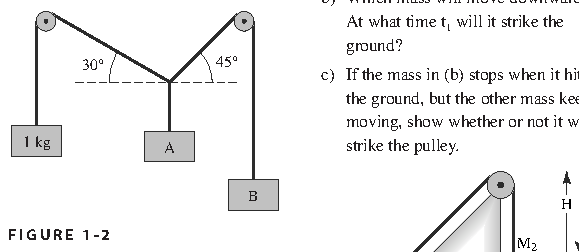
\includegraphics[width=0.86\linewidth,height=0.42\textheight,keepaspectratio]{../assets/pdf-layer-figures/fig-1_2-p173.pdf}

\par{\scriptsize Рисунок 1-2 (исходная стр. 173)}

\end{center}

\begin{center}

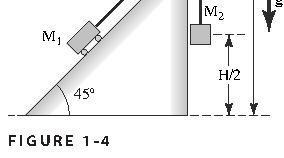
\includegraphics[width=0.86\linewidth,height=0.42\textheight,keepaspectratio]{../assets/pdf-layer-figures/fig-1_4-p173.pdf}

\par{\scriptsize Рисунок 1-4 (исходная стр. 173)}

\end{center}

\begin{center}

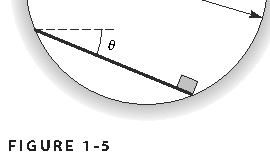
\includegraphics[width=0.86\linewidth,height=0.42\textheight,keepaspectratio]{../assets/pdf-layer-figures/fig-1_5-p173.pdf}

\par{\scriptsize Рисунок 1-5 (исходная стр. 173)}

\end{center}

\begin{center}

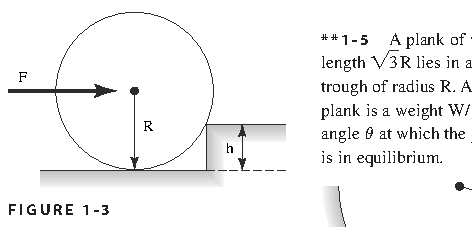
\includegraphics[width=0.86\linewidth,height=0.42\textheight,keepaspectratio]{../assets/pdf-layer-figures/fig-1_3-p173.pdf}

\par{\scriptsize Рисунок 1-3 (исходная стр. 173)}

\end{center}



И З Б Р А Н Н Ы Е  У П Р А Ж Н Е Н И Я • 1 5 7 Вид сбоку Вид сверху \emph{ } 1 - 7 Катушка массой состоит из центрального цилиндра радиуса 5 см и двух боковых дисков радиуса Она помещена на наклонную плоскость с прорезью, по которой она будет катиться без проскальзывания, а масса подвешена на нити, намотанной вокруг катушки. Наблюдается, что система находится в статическом равновесии. Чему равен угол наклона плоскости? \(\theta\) m = 4,5 кг R = 6 см. r = M = 3 кг r R M m \(\theta\) \(\theta\) w W \emph{ } 1 - 8 Тележка на наклонной плоскости уравновешена весом w. Трением во всех частях можно пренебречь. Найдите вес W тележки. \emph{ } 1 - 9 В баке с площадью поперечного сечения A находится жидкость плотности Жидкость свободно вытекает из малого отверстия площадью a на расстоянии H под свободной поверхностью жидкости. Если жидкость не имеет внутреннего трения (вязкости), с какой скоростью она вытекает? \textbackslash{}rho. Р И С У Н О К  1 - 6 Р И С У Н О К  1 - 7 Р И С У Н О К  1 - 8 H Р И С У Н О К  1 - 9 \emph{ } 1 - 6 Украшение для двора на Всемирной выставке должно состоять из четырех одинаковых гладких металлических сфер, каждая весом тс. Сферы должны быть расположены, как показано на рисунке: три лежат на горизонтальной поверхности и касаются друг друга, а четвертая свободно лежит на трех других. Три нижние удерживаются от расхождения точечной сваркой в точках их соприкосновения. С учетом коэффициента запаса прочности, равного 3, какое натяжение должны выдерживать сварные точки? \(2\sqrt{6}\)\par

\begin{center}

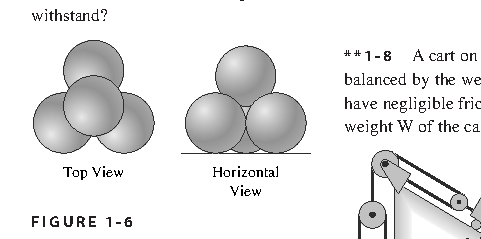
\includegraphics[width=0.86\linewidth,height=0.42\textheight,keepaspectratio]{../assets/pdf-layer-figures/fig-1_6-p174.pdf}

\par{\scriptsize Рисунок 1-6 (исходная стр. 174)}

\end{center}

\begin{center}

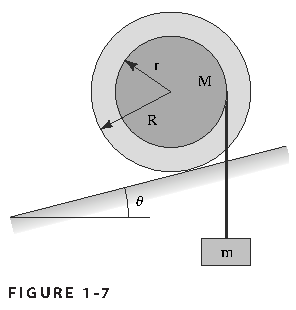
\includegraphics[width=0.86\linewidth,height=0.42\textheight,keepaspectratio]{../assets/pdf-layer-figures/fig-1_7-p174.pdf}

\par{\scriptsize Рисунок 1-7 (исходная стр. 174)}

\end{center}

\begin{center}

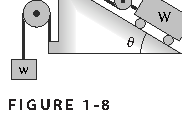
\includegraphics[width=0.86\linewidth,height=0.42\textheight,keepaspectratio]{../assets/pdf-layer-figures/fig-1_8-p174.pdf}

\par{\scriptsize Рисунок 1-8 (исходная стр. 174)}

\end{center}

\begin{center}

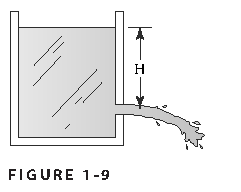
\includegraphics[width=0.86\linewidth,height=0.42\textheight,keepaspectratio]{../assets/pdf-layer-figures/fig-1_9-p174.pdf}

\par{\scriptsize Рисунок 1-9 (исходная стр. 174)}

\end{center}



1 5 8 • Г Л А В А  5 Земли со спутником. Если P лежит на пересечении этой линии с земной поверхностью, может ли P иметь любую географическую широту или существуют какие-то ограничения? Объясните. б) Каково расстояние от центра Земли до спутника Syncom массой m? Выразите в единицах расстояния от Земли до Луны Примечание: Считайте Землю однородным шаром. Вы можете использовать для периода обращения Луны. Tm = 27 дней rem . rs rs \emph{ 2 - 1 Эксцентриситет земной орбиты равен 0,0167. Найдите отношение ее максимальной скорости на орбите к ее минимальной скорости. } \emph{ 2 - 2 Настоящий спутник «Syncom» (геосинхронный) вращается синхронно с Землей. Он всегда остается в фиксированном положении относительно точки P на земной поверхности. а) Рассмотрим прямую линию, соединяющую центр 5-2 Законы Кеплера и тяготение (Т. I, гл. 7) 5-3 Кинематика (Т. I, гл. 8) } 3 - 1 Аэростат Skyhook с научной аппаратурой поднимается со скоростью 1000 футов в минуту. На высоте 30 000 футов аэростат лопается, и аппаратура переходит в свободное падение. (Такие катастрофы действительно случаются!) а) Какое время аппаратура находилась в воздухе? б) Какова была скорость аппаратуры при ударе? Пренебречь сопротивлением воздуха. \emph{ 3 - 2 Рассмотрите поезд, который может ускоряться с ускорением 20 см/ и замедляться с замедлением 100 см/ Найдите минимальное время движения поезда между двумя станциями, расположенными на расстоянии 2 км друг от друга. с². с² } 3 - 3 Если бросить маленький мяч вертикально вверх в реальном воздухе с сопротивлением, понадобится ли ему больше времени на подъем или на спуск? \emph{ } 3 - 4 В лекционной демонстрации маленький стальной шарик прыгает на стальной плите. При каждом отскоке направленная вниз скорость шарика при подлете к плите уменьшается в e раз при отскоке, т. е. Если изначально шарик отпустили с высоты 50 см над плитой в момент времени и если 30 секунд спустя затихание звука в микрофоне показало, что все отскоки прекратились, каково было значение e? t = 0, vвверх = e * vвниз .\par



И З Б Р А Н Н Ы Е  У П Р А Ж Н Е Н И Я • 1 5 9 \emph{ } 3 - 5 Водитель автомобиля едет за грузовиком и вдруг замечает, что между двумя задними шинами грузовика застрял камень. Будучи осторожным водителем (и к тому же физиком), он тут же увеличивает дистанцию до грузовика до 22,5 метров, чтобы в него не попал камень в случае, если он вылетит. С какой скоростью ехал грузовик? (Считайте, что камень после удара о землю не отскакивает.) \emph{ } * 3-6 Первокурсник Калифорнийского технологического института, не имеющий опыта общения с пригородными дорожными инспекторами, только что получил штраф за превышение скорости. После этого, когда он выезжает на один из участков «Проверки спидометра» на ровном отрезке шоссе, он решает проверить показания своего спидометра. Проезжая начальную отметку «0» размеченного участка, он нажимает на педаль акселератора и в течение всего времени проверки поддерживает постоянное ускорение автомобиля. Он замечает, что проезжает отметку 0,10 мили через 16 секунд после начала проверки, а еще через 8,0 секунд проезжает отметку 0,20 мили. a) Что должен был показывать его спидометр на отметке 0,20 мили? б) Каково было его ускорение? 5-4 Законы Ньютона (т. I, гл. 9) Р И С У Н О К  4 - 1 \emph{ } * 3 - 7 На длинном горизонтальном испытательном треке авиабазы Эдвардс можно испытывать как ракетные, так и реактивные двигатели. В один из дней ракетный двигатель, запущенный из состояния покоя, ускорялся с постоянным ускорением, пока не выработалось топливо, после чего он двигался с постоянной скоростью. Было замечено, что топливо полностью выработалось в тот момент, когда ракета прошла середину измеряемой дистанции испытания. Затем с начала трека из состояния покоя был запущен реактивный двигатель, двигавшийся с постоянным ускорением на протяжении всей дистанции. Было замечено, что и ракетный, и реактивный двигатели прошли испытательную дистанцию за абсолютно одинаковое время. Каково отношение ускорения реактивного двигателя к ускорению ракетного двигателя? * 4 - 1 Два тела массой m = 1 кг каждое, соединенные натянутой нитью длиной L = 2 м, движутся по круговой орбите с постоянной скоростью V = 5 м/с вокруг их общего центра C в условиях невесомости. Каково натяжение нити в ньютонах? C V V\par

\begin{center}

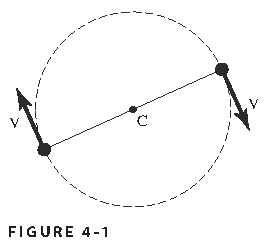
\includegraphics[width=0.86\linewidth,height=0.42\textheight,keepaspectratio]{../assets/pdf-layer-figures/fig-4_1-p176.pdf}

\par{\scriptsize Рисунок 4-1 (исходная стр. 176)}

\end{center}



1 6 0 • Г Л А В А  5 M M P T M h m C Р И С У Н О К  4 - 3 Р И С У Н О К  4 - 4 M с каждой стороны, как показано на рисунке (сплошная линия), а затем с одной стороны добавляется небольшой перегрузок m. Объединенные массы ускоряются на некотором расстоянии h, после чего перегрузок задерживается кольцом, и две равные массы продолжают движение с постоянной скоростью v. Найдите значение g, соответствующее измеренным значениям m, M, h и v. \emph{ } * 4 - 4 Маляр весом 180 фунтов, работающий в подвесной люльке («боцманском стуле»), висящей на стене высокого здания, хочет срочно подняться. Он тянет ходовой конец каната вниз с такой силой, что давит на люльку с силой всего лишь 100 фунтов. Сама люлька весит 30,0 фунтов. a) Каково ускорение маляра и люльки? б) Какова общая сила, действующая на блок? Р И С У Н О К  4 - 2 \emph{ } 4 - 2 Какую горизонтальную силу F необходимо постоянно прикладывать к M, чтобы M1 и M2 не двигались относительно M? Трением пренебречь. M2 M1 M2 M1 F M \emph{ } 4 - 3 На рисунке показана машина Атвуда --- один из первых приборов для измерения ускорения свободного падения. Блок P и нить C имеют пренебрежимо малую массу и трение. Система уравновешена одинаковыми массами\par

\begin{center}

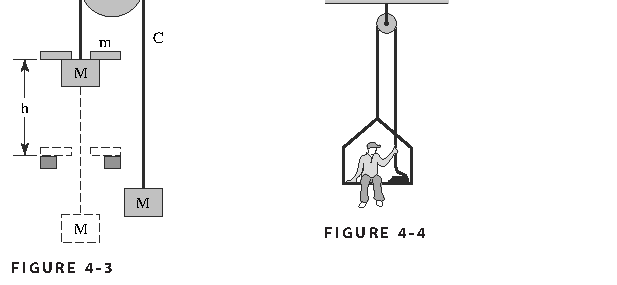
\includegraphics[width=0.86\linewidth,height=0.42\textheight,keepaspectratio]{../assets/pdf-layer-figures/fig-4_3-p177.pdf}

\par{\scriptsize Рисунок 4-3 (исходная стр. 177)}

\end{center}

\begin{center}

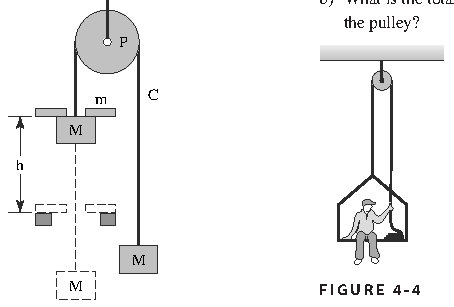
\includegraphics[width=0.86\linewidth,height=0.42\textheight,keepaspectratio]{../assets/pdf-layer-figures/fig-4_4-p177.pdf}

\par{\scriptsize Рисунок 4-4 (исходная стр. 177)}

\end{center}

\begin{center}

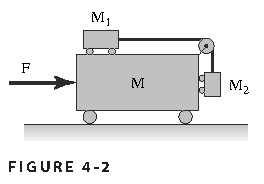
\includegraphics[width=0.86\linewidth,height=0.42\textheight,keepaspectratio]{../assets/pdf-layer-figures/fig-4_2-p177.pdf}

\par{\scriptsize Рисунок 4-2 (исходная стр. 177)}

\end{center}



И З Б Р А Н Н Ы Е  У П Р А Ж Н Е Н И Я • 1 6 1 5-5 Закон сохранения импульса (т. I, гл. 10) \emph{ 5 - 1 Две тележки могут свободно двигаться по горизонтальному воздушному треку. Одна из них неподвижна, а другая сталкивается с ней абсолютно упруго. Они отскакивают с равными по модулю и противоположными по направлению скоростями. Каково отношение их масс? } * 5 - 2 Пулемет, установленный на северном конце платформы массой 10 000 кг и длиной 5 м, которая может свободно перемещаться на горизонтальной воздушной подушке, стреляет пулями в толстую мишень, закрепленную на южном конце платформы. Пулемет выпускает 10 пуль массой 100 г каждая каждую секунду с начальной скоростью 500 м/с. a) Двигается ли платформа? б) В каком направлении? в) С какой скоростью? \emph{ } 5 - 3 Конец цепи с массой на единицу длины m, покоящейся на столе при t = 0, поднимают вертикально вверх с постоянной скоростью v. Найдите силу натяжения при подъеме как функцию времени. Р И С У Н О К  5 - 3 Р И С У Н О К  4 - 5 B A \emph{ } * 4 - 5 Космический путешественник, собирающийся отправиться на Луну, имеет пружинные весы и гирю A массой 1,0 кг, которая при взвешивании на Земле показывает 9,8 ньютона. Прибыв на Луну в место, где ускорение свободного падения точно неизвестно, но составляет около 1/6 от ускорения свободного падения на поверхности Земли, он берет камень B, который при взвешивании на тех же пружинных весах показывает 9,8 ньютона. Затем он подвешивает гирю A и камень B через блок, как показано на рисунке, и замечает, что камень B опускается с ускорением 1,2 м/с². Какова масса камня B?\par

\begin{center}

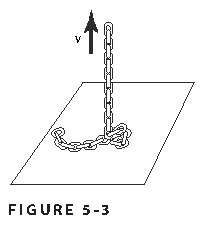
\includegraphics[width=0.86\linewidth,height=0.42\textheight,keepaspectratio]{../assets/pdf-layer-figures/fig-5_3-p178.pdf}

\par{\scriptsize Рисунок 5-3 (исходная стр. 178)}

\end{center}

\begin{center}

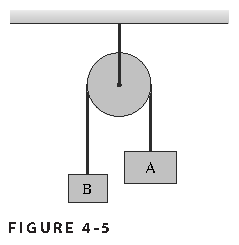
\includegraphics[width=0.86\linewidth,height=0.42\textheight,keepaspectratio]{../assets/pdf-layer-figures/fig-4_5-p178.pdf}

\par{\scriptsize Рисунок 4-5 (исходная стр. 178)}

\end{center}



1 6 2 • Г Л А В А  5 M L V m x \emph{ } * 5 - 4 Скорость ружейной пули можно измерить с помощью баллистического маятника. Пуля известной массы m и неизвестной скорости V застревает в неподвижном деревянном бруске массой M, подвешенном как маятник длиной L. Это приводит брусок в движение. Амплитуду колебаний x можно измерить и, используя закон сохранения энергии, найти скорость бруска сразу после удара. Выразите скорость пули через m, M, L и x. Р И С У Н О К  5 - 4 \emph{ } * 5 - 5 Две одинаковые тележки, движущиеся по горизонтальному воздушному треку с равными и противоположными скоростями v и -v, сталкиваются почти упруго и отскакивают с немного меньшими скоростями. При столкновении они теряют долю f << 1 своей кинетической энергии. Если эти же тележки сталкиваются, причем одна из них первоначально покоится, то с какой скоростью будет двигаться первая тележка после столкновения? (Эту небольшую остаточную скорость Δv можно легко измерить через конечную скорость v первоначально покоившейся тележки, и таким образом определить упругость пружинных буферов.) Примечание: Если x << 1, то (1 - x)\textasciicircum{}(1/2) \ensuremath{\approx} 1 - (1/2)x. \emph{ } * 5 - 6 Спутник Земли массой 10 кг и средней площадью поперечного сечения 0,50 м² движется по круговой орбите на высоте 200 км, где длина свободного пробега молекул составляет многие метры, а плотность воздуха равна примерно 10\textasciicircum{}(-10) кг/м³. В грубом предположении, что соударения молекул со спутником являются абсолютно неупругими (но при этом молекулы не прилипают к спутнику буквально, а отлетают от него с малым относительным скоростями), вычислите силу торможения, которую испытывает спутник из-за трения о воздух. Как эта сила трения должна зависеть от скорости? Будет ли скорость спутника уменьшаться в результате действия на него результирующей силы? (Проверьте зависимость скорости спутника на круговой орбите от высоты.)\par

\begin{center}

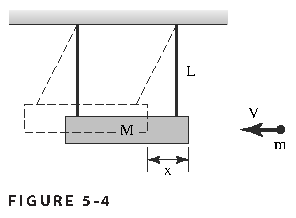
\includegraphics[width=0.86\linewidth,height=0.42\textheight,keepaspectratio]{../assets/pdf-layer-figures/fig-5_4-p179.pdf}

\par{\scriptsize Рисунок 5-4 (исходная стр. 179)}

\end{center}



И З Б Р А Н Н Ы Е  У П Р А Ж Н Е Н И Я • 1 6 3 5-6 Векторы (Т. I, гл. 11) H m \emph{ } * 6 - 4 Вы находитесь на корабле, идущем постоянным курсом на восток со скоростью 15 узлов. Другой корабль, идущий постоянным курсом, скорость которого известна и составляет 26 узлов, обнаружен в 6,0 мили строго к югу от вас; позже замечено, что он проходит позади вас, причем расстояние наибольшего сближения составляет 3,0 мили. а) Каков был курс другого корабля? б) Сколько времени прошло между его положением к югу от вас и положением наибольшего сближения? Р И С У Н О К  6 - 3 \emph{ } 6 - 1 Человек, стоящий на берегу реки шириной 1,0 мили, хочет добраться до точки, расположенной прямо напротив него на другом берегу. Он может сделать это двумя способами: (1) направляться несколько против течения, так чтобы его результирующее движение было направлено прямо поперек, (2) направляться к противоположному берегу, а затем идти пешком вверх по берегу от точки ниже по течению, куда его снесет течение. Если он может плыть и идти пешком и если скорость течения составляет какой способ переправы быстрее и на сколько? \emph{ } 6 - 2 Моторная лодка, идущая с постоянной скоростью V относительно воды, движется в прямом русле реки, где вода течет спокойно с постоянной скоростью R. Сначала лодку отправляют в рейс туда и обратно от места ее стоянки до точки на расстоянии d прямо вверх по течению. Затем ее отправляют в рейс туда и обратно от места стоянки до точки на расстоянии d прямо поперек течения. Для простоты предположим, что в обоих случаях лодка проходит все расстояние на полной скорости и что время на изменение направления в конце пути в одну сторону не теряется. Если --- время, затраченное лодкой на рейс туда и обратно вдоль течения реки, --- время, затраченное лодкой на рейс туда и обратно поперек течения, и --- время, которое потребовалось бы лодке, чтобы пройти расстояние 2d по озеру. а) Чему равно отношение б) Чему равно отношение tA/tL ? tV/tA ? tL tA tV 2,0 мили/ч, 4,0 мили/ч, 2,5 мили/ч \emph{ } 6 - 3 Масса m подвешена к подвесу без трения на конце нити произвольной длины и приведена во вращение по горизонтальной круговой траектории, плоскость которой находится на расстоянии H ниже точки подвеса. Найдите период обращения массы по ее орбите.\par

\begin{center}

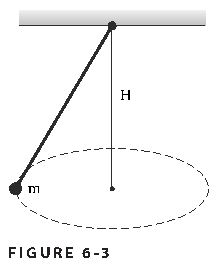
\includegraphics[width=0.86\linewidth,height=0.42\textheight,keepaspectratio]{../assets/pdf-layer-figures/fig-6_3-p180.pdf}

\par{\scriptsize Рисунок 6-3 (исходная стр. 180)}

\end{center}



1 6 4 • Г Л А В А  5 5-8 Силы (Т. I, гл. 12) \emph{ 8 - 1 Две массы, и связаны нитями пренебрежимо малого веса, перекинутыми через практически лишенные трения блоки, с третьей массой, Масса движется по длинному столу с коэффициентом трения m2 m2 = 2 кг. m3 = 2 кг, m1 = 4 кг Каково ускорение массы после того, как система отпущена из состояния покоя? } * 8 - 2 Пуля массой 5 г выпущена горизонтально в деревянный брусок массой 3 кг, покоящийся на горизонтальной поверхности. Коэффициент трения скольжения между бруском и поверхностью равен 0,2. Пуля остается застрявшей в бруске, который, как замечено, проскальзывает на 25 см по поверхности. Какова была скорость пули? m1 μ = 1/2. m1 m3 m2 Р И С У Н О К  8 - 1 \emph{ } 7 - 1 Движущаяся частица массы M испытывает абсолютно упругое столкновение с покоящейся частицей массы Найдите максимально возможный угол, на который может отклониться налетающая частица. \emph{ } 7 - 2 Тело массы движущееся с линейной скоростью v в лабораторной системе, сталкивается с телом массы которое покоится в лабораторной системе. После столкновения m2 m1 , m < M. замечено, что доля кинетической энергии в системе ЦМ была потеряна при столкновении. Какова процентная потеря энергии в лабораторной системе? \emph{ } 7 - 3 Протон с кинетической энергией 1 МэВ испытывает упругое столкновение с покоящимся ядром и отклоняется на Если теперь энергия протона составляет 0,80 МэВ, какова была масса ядра-мишени в единицах массы протона? 90°. (1 - a\textasciicircum{}2) 5-7 Нерелятивистские двухчастичные столкновения в 3 измерениях (Т. I, гл. 10 и 11)\par

\begin{center}

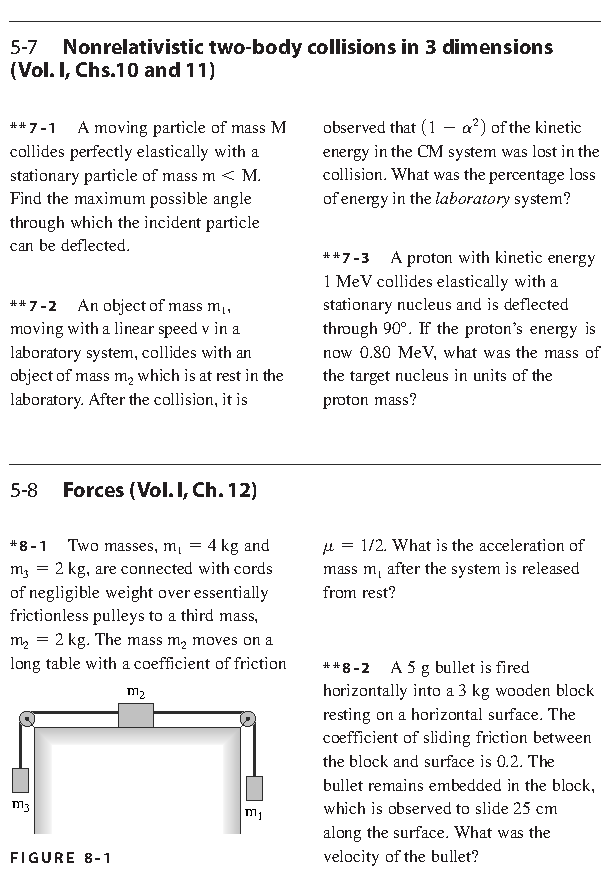
\includegraphics[width=0.86\linewidth,height=0.42\textheight,keepaspectratio]{../assets/pdf-layer-figures/fig-8_1-p181.pdf}

\par{\scriptsize Рисунок 8-1 (исходная стр. 181)}

\end{center}



И З Б Р А Н Н Ы Е  У П Р А Ж Н Е Н И Я • 1 6 5 5-9 Потенциалы и поля (Т. I, гл. 13 и 14) \emph{ 9 - 1 Масса m сталкивается с пружиной жесткостью k. В какой точке она впервые останавливается? Массой пружины пренебречь. } * 8 - 3 При расследовании на месте автомобильной аварии полиция установила путем измерений, что автомобиль A оставил тормозной след длиной 150 футов перед столкновением с автомобилем B. Также было известно, что коэффициент трения между резиной и дорожным покрытием на месте аварии был не менее 0,6. Покажите, что скорость автомобиля A непосредственно перед аварией должна была превышать установленный предел 45 миль/ч. (Обратите внимание, что и ускорение свободного падения \emph{ } 8 - 4 Школьный автобус с кондиционером приближается к железнодорожному переезду. Один из детей привязал к сиденью наполненный водородом шарик. Вы замечаете, что нить, удерживающая шарик, составляет угол с вертикалью в направлении движения. Тормозит или ускоряет водитель автобус, и на сколько? (Похвалил бы патрульный полицейский водителя за его мастерство?) 30° g = 60 миль/ч = 88 футов/с 30° a H Р И С У Н О К  8 - 4 Р И С У Н О К  8 - 5 Р И С У Н О К  9 - 1 m v0 x0 Гладкая x k \emph{ } * 8 - 5 Частица весом W покоится на шероховатой наклонной плоскости, составляющей угол с горизонталью. a) Если коэффициент трения покоя найдите наименьшую горизонтальную силу действующую поперек склона плоскости, которая заставит частицу двигаться. б) В каком направлении она начнет движение? Hmin , μ = 2 tan a, a Потенциалы и поля (Т. I, гл. 13 и 14)\par

\begin{center}

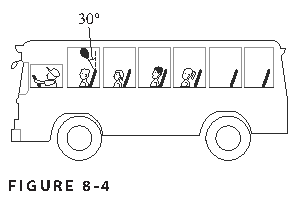
\includegraphics[width=0.86\linewidth,height=0.42\textheight,keepaspectratio]{../assets/pdf-layer-figures/fig-8_4-p182.pdf}

\par{\scriptsize Рисунок 8-4 (исходная стр. 182)}

\end{center}

\begin{center}

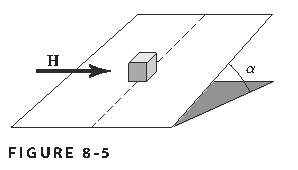
\includegraphics[width=0.86\linewidth,height=0.42\textheight,keepaspectratio]{../assets/pdf-layer-figures/fig-8_5-p182.pdf}

\par{\scriptsize Рисунок 8-5 (исходная стр. 182)}

\end{center}

\begin{center}

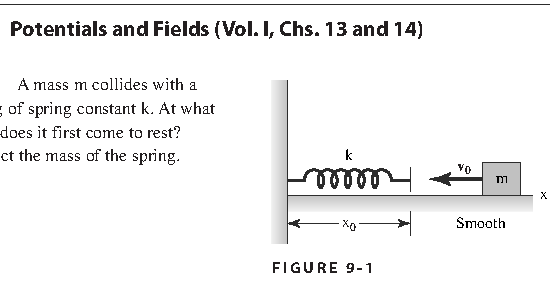
\includegraphics[width=0.86\linewidth,height=0.42\textheight,keepaspectratio]{../assets/pdf-layer-figures/fig-9_1-p182.pdf}

\par{\scriptsize Рисунок 9-1 (исходная стр. 182)}

\end{center}



1 6 6 • Г Л А В А  5 \emph{ } 9 - 6 Частица начинает движение из состояния покоя на вершине гладкой (без трения) сферы радиуса R и скользит по сфере под действием силы тяжести. На сколько опустится частица по вертикали относительно начальной точки, прежде чем оторвется от сферы? \emph{ } 9 - 7 Автомобиль массой 1000 кг приводится в движение двигателем, номинальная мощность которого составляет 120 кВт. Если двигатель развивает эту мощность при скорости 60 км/ч, каково максимальное ускорение, которое автомобиль может иметь при этой скорости? \emph{ } 9 - 8 Мировые рекорды (1960 г.) по толканию ядра, метанию диска и копья составляли соответственно 19,30 м, 59,87 м и 86,09 м. Массы используемых снарядов равны соответственно 7,25 кг, 2 кг и 0,8 кг. Сравните работу, совершенную каждым чемпионом при рекордном броске, считая, что каждая траектория начинается на высоте 1,80 м над уровнем земли и имеет начальный угол наклона к горизонту 45°. Сопротивлением воздуха пренебречь. \emph{ } \emph{ 9 - 9 Спутник массой m движется по круговой орбите вокруг астероида массой M (M >> m). Если бы масса астероида внезапно² уменьшилась вдвое по сравнению с прежним значением, что произошло бы со спутником? Опишите его новую орбиту. } 9 - 2 Полый сферический астероид свободно движется в космосе. Внутри него находится маленькая частица массой m. В какой точке внутри астероида частица будет находиться в положении равновесия? * 9 - 3 Скорость, необходимая телу для того, чтобы покинуть гравитационное поле Земли, составляет (приблизительно) 7,0 миль/с. Если межпланетному зонду сообщить начальную скорость 8,0 миль/с непосредственно над земной атмосферой, с какой скоростью относительно Земли он будет двигаться, когда будет находиться на расстоянии 10⁶ миль от Земли? \emph{ 9 - 4 Маленькая тележка без трения скатывается по наклонной дорожке, заканчивающейся круговой «мертвой петлей» радиуса R в нижней части. С какой высоты H над верхней точкой петли должна стартовать тележка, чтобы пройти всю петлю, не отрываясь от трека? } 9 - 5 Гибкий кабель длиной L и массой единицы длины M кг/м висит на шкиве, масса, радиус и трение которого пренебрежимо малы. Первоначально кабель находится в точном равновесии. Ему сообщают небольшой толчок, выводящий его из равновесия, и он начинает ускоряться. Найдите его скорость в момент, когда его конец слетает со шкива.\par



² Как это могло произойти: Спутник выводится на орбиту на большом расстоянии от астероида для наблюдения за испытанием ядерного устройства на астероиде. Взрыв выбрасывает половину массы астероида, не оказывая прямого воздействия на удаленный спутник.\par



И З Б Р А Н Н Ы Е  У П Р А Ж Н Е Н И Я • 1 6 7 5-10 Единицы и размерности (т. I, гл. 5) * 1 0 - 1 Мо и Джо, два космических физика, выросших на разных планетах, встречаются на межпланетном симпозиуме по мерам и весам, чтобы обсудить создание универсальной системы единиц. Мо с гордостью описывает достоинства системы МКСА, используемой во всех цивилизованных областях Земли. Джо столь же гордо описывает прелести системы MrKrSrAr, используемой повсеместно в остальных частях Солнечной системы. Если постоянные коэффициенты, связывающие основные эталоны массы, длины и времени двух систем, равны μ, λ и τ, так что mr = μm, lr = λl и tr = τt, то какие коэффициенты необходимы для перевода единиц скорости, ускорения, силы и энергии из одной системы в другую? \emph{ } 1 0 - 2 Если создать масштабную модель Солнечной системы, используя материалы с такими же средними плотностями, как у Солнца и планет, но уменьшив все линейные размеры в k раз (коэффициент масштабирования k), то как периоды обращения планет будут зависеть от k? \emph{ 1 1 - 1 а) Выразите импульс частицы через ее кинетическую энергию T и энергию покоя m₀c². б) Какова скорость частицы, кинетическая энергия которой равна ее энергии покоя? } \emph{ 1 1 - 2 Покоящийся пион (mp = 273 me) распадается на мюон (mm = 207 me) и нейтрино (mn = 0). Найдите кинетическую энергию и импульс мюона и нейтрино в МэВ. 5-11 Релятивистская энергия и импульс (т. I, гл. 16 и 17) } \emph{ 1 1 - 3 Частица массой m, движущаяся со скоростью v = 4c/5, претерпевает неупругое столкновение с такой же покоящейся частицей. а) Какова скорость образовавшейся составной частицы? б) Какова ее масса? } * 1 1 - 4 Протон-антипротонная пара может родиться при поглощении фотона (γ) покоящимся протоном: γ + p \ensuremath{\to} p + p + p̄. Какую минимальную энергию E\_γ должен иметь фотон? (Выразите E\_γ через энергию покоя протона mp c²).\par



1 6 8 • Г Л А В А  5 \emph{ } 1 2 - 4 Массы M₁ и M₂ помещены на противоположных концах жесткого стержня длиной L и пренебрежимо малой массы; размеры M₁ и M₂ пренебрежимо малы по сравнению с L. Стержень приводится во вращение вокруг перпендикулярной ему оси. Через какую точку стержня должна проходить эта ось, чтобы работа, необходимая для приведения стержня во вращение с угловой скоростью ω₀, была минимальной? \emph{ } * 1 2 - 5 Однородный кирпич длиной L лежит на гладкой горизонтальной поверхности. Сверху на него укладывают другие такие же кирпичи, как показано на рисунке, так что их боковые грани образуют непрерывные плоскости, но торцы каждого последующего кирпича смещены относительно предыдущего на расстояние L/a, где a --- целое число. Сколько кирпичей можно уложить таким способом, прежде чем стопка опрокинется? 5-12 Двумерные вращения, центр масс (т. I, гл. 18 и 19) \emph{ } 1 2 - 1 Из однородного диска вырезано круглое отверстие, как показано на рисунке. Найдите центр масс. Р И С У Н О К  1 2 - 5 x y 20 см. 10 см. \emph{ } 1 2 - 2 Сплошной цилиндр имеет плотность, меняющуюся по квадрантам, как показано на рисунке, где числа указывают относительные плотности. Если оси x-y направлены так, как показано на рисунке, каково уравнение прямой, проходящей через начало координат и центр масс? Р И С У Н О К  1 2 - 1 Р И С У Н О К  1 2 - 2 Р И С У Н О К  1 2 - 3 \emph{ } 1 2 - 3 Из квадратного листа однородного листового металла со стороны одного из краев вырезается равнобедренный треугольник, как показано на рисунке, таким образом, чтобы оставшаяся часть металла при подвешивании за вершину выреза P оставалась в равновесии в любом положении. Какова высота вырезанного треугольника?\par

\begin{center}

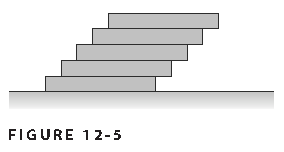
\includegraphics[width=0.86\linewidth,height=0.42\textheight,keepaspectratio]{../assets/pdf-layer-figures/fig-12_5-p185.pdf}

\par{\scriptsize Рисунок 12-5 (исходная стр. 185)}

\end{center}

\begin{center}

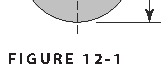
\includegraphics[width=0.86\linewidth,height=0.42\textheight,keepaspectratio]{../assets/pdf-layer-figures/fig-12_1-p185.pdf}

\par{\scriptsize Рисунок 12-1 (исходная стр. 185)}

\end{center}

\begin{center}

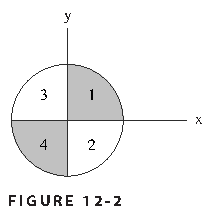
\includegraphics[width=0.86\linewidth,height=0.42\textheight,keepaspectratio]{../assets/pdf-layer-figures/fig-12_2-p185.pdf}

\par{\scriptsize Рисунок 12-2 (исходная стр. 185)}

\end{center}

\begin{center}

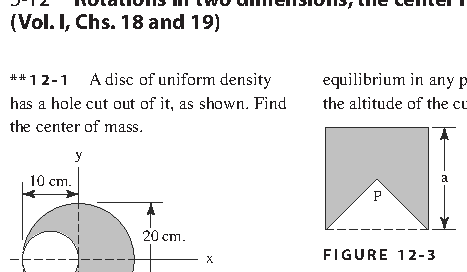
\includegraphics[width=0.86\linewidth,height=0.42\textheight,keepaspectratio]{../assets/pdf-layer-figures/fig-12_3-p185.pdf}

\par{\scriptsize Рисунок 12-3 (исходная стр. 185)}

\end{center}



И З Б Р А Н Н Ы Е  З А Д А Ч И • 1 6 9 \emph{ } * 1 2 - 6 Показанный на рисунке центробежный регулятор предназначен для отключения питания, когда машина, с которой он непосредственно связан, достигает скорости вращения 120 об/мин. Рабочая муфта C весит 10,0 фунта и скользит без трения по вертикальному валу AB. Муфта C устроена так, чтобы отключать питание, когда расстояние AC уменьшается до 1,41 фута. Если четыре тяги рамы регулятора имеют длину 1,00 фута каждая между шарнирами без трения и их массой можно пренебречь, то какова должна быть масса M грузов, чтобы регулятор работал так, как запланировано? A M M B C Р И С У Н О К  1 2 - 6 5-13 Момент импульса, момент инерции (т. I, гл. 18 и 19) \emph{ 1 3 - 1 Прямая однородная проволока длины L и массы M согнута посередине, образуя угол Каков ее момент инерции относительно оси, проходящей через точку А перпендикулярно плоскости, определяемой согнутой проволокой? u. } 1 3 - 2 Груз массы m подвешен на нити, намотанной на сплошной круглый цилиндр массы M и радиуса r, который вращается на подшипниках с пренебрежимо малым трением, как показано на рисунке. Найдите ускорение груза m. A u Р И С У Н О К  1 3 - 1 M m r Р И С У Н О К  1 3 - 2 (т. I, гл. 18 и 19)\par

\begin{center}

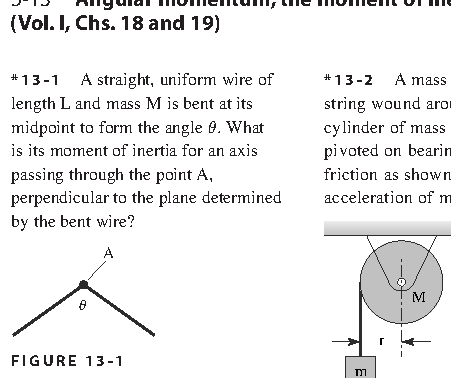
\includegraphics[width=0.86\linewidth,height=0.42\textheight,keepaspectratio]{../assets/pdf-layer-figures/fig-13_1-p186.pdf}

\par{\scriptsize Рисунок 13-1 (исходная стр. 186)}

\end{center}

\begin{center}

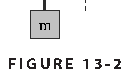
\includegraphics[width=0.86\linewidth,height=0.42\textheight,keepaspectratio]{../assets/pdf-layer-figures/fig-13_2-p186.pdf}

\par{\scriptsize Рисунок 13-2 (исходная стр. 186)}

\end{center}



1 7 0 • Г Л А В А  5 \emph{ } 1 3 - 4 Начиная движение из состояния покоя, симметричное тело скатывается (без проскальзывания) по наклонной плоскости высоты h. Момент инерции тела относительно его центра масс равен I, масса равна M, а радиус поверхности качения, соприкасающейся с наклонной плоскостью, равен r. Определите линейную скорость центра масс в конце наклонной плоскости. \emph{ } 1 3 - 5 На бесконечную ленту, которая наклонена под углом к горизонтали, помещен однородный цилиндр, ось которого горизонтальна и перпендикулярна краю ленты. u h H P d Р И С У Н О К  1 3 - 6 \emph{ } 1 3 - 3 Тонкий горизонтальный стержень массы M и длины L одним концом лежит на опоре, а другим подвешен на нити. Какую силу прикладывает стержень к опоре сразу после пережигания нити? Р И С У Н О К  1 3 - 3 \emph{ } * 1 3 - 7 Однородный шар для боулинга радиуса R и массы M запускают так, что первоначально он скользит со скоростью без качения по дорожке с коэффициентом трения Как далеко уедет шар, прежде чем начнет катиться без проскальзывания, и какова будет его скорость в этот момент? μ. V0 Свойства поверхностей таковы, что цилиндр может катиться без проскальзывания по ленте. Как следует приводить ленту в движение, чтобы после того, как цилиндр отпустят, ось цилиндра оставалась неподвижной? \emph{ } 1 3 - 6 Обруч H радиуса r скатывается без проскальзывания по наклонной плоскости. Начальная высота h такова, что обруч приобретает скорость, как раз достаточную для прохождения «мертвой петли» --- то есть обруч едва удерживает контакт с круговой дорожкой в точке P. Чему равно h?\par

\begin{center}

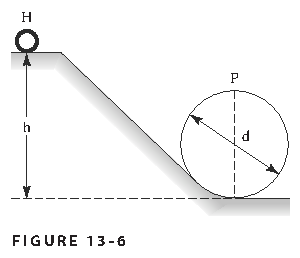
\includegraphics[width=0.86\linewidth,height=0.42\textheight,keepaspectratio]{../assets/pdf-layer-figures/fig-13_6-p187.pdf}

\par{\scriptsize Рисунок 13-6 (исходная стр. 187)}

\end{center}

\begin{center}

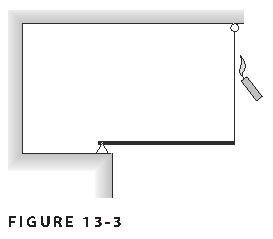
\includegraphics[width=0.86\linewidth,height=0.42\textheight,keepaspectratio]{../assets/pdf-layer-figures/fig-13_3-p187.pdf}

\par{\scriptsize Рисунок 13-3 (исходная стр. 187)}

\end{center}



И З Б Р А Н Н Ы Е  З А Д А Ч И • 1 7 1 V0 v0 Р И С У Н О К  1 3 - 8 \emph{ } * 1 3 - 8 Забавный трюк состоит в том, чтобы прижать пальцем шарик на горизонтальной поверхности стола таким образом, чтобы шарик полетел вдоль стола с начальной линейной скоростью и начальной угловой скоростью обратного вращения вокруг горизонтальной оси, перпендикулярной Коэффициент трения скольжения между шариком и поверхностью стола постоянен. Шарик имеет радиус R. а) Какое соотношение должно выполняться между R и , чтобы шарик проскользил до полной остановки? v0 V0 , V0 . v0 v0 , V0 5-14 Вращение в трех измерениях (т. I, гл. 20) б) Какое соотношение должно выполняться между R и , чтобы шарик проскользил до остановки, а затем начал возвращаться к своему начальному положению с конечной постоянной линейной скоростью 3/7 V0 ? v0 V0 , * 1 4 - 1 Реактивный самолет, все двигатели которого вращаются в направлении правого винта, движущегося в направлении полета, выполняет левый разворот. Стремится ли гироскопический эффект двигателей вызвать: а) крен вправо б) крен влево в) рыскание вправо г) рыскание влево д) кабрирование (подъем носа) е) пикирование (опускание носа) \emph{ } 1 4 - 2 Две равные массы соединены гибкой нитью. Экспериментатор держит одну массу в руке и заставляет другую вращаться по горизонтальной окружности вокруг удерживаемой массы; затем он отпускает удерживаемую массу. а) Если во время эксперимента нить рвется, то порвалась ли она до или после того, как он отпустил массы? б) Если нить не рвется, опишите движение масс после того, как их отпустили.\par

\begin{center}

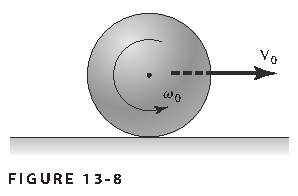
\includegraphics[width=0.86\linewidth,height=0.42\textheight,keepaspectratio]{../assets/pdf-layer-figures/fig-13_8-p188.pdf}

\par{\scriptsize Рисунок 13-8 (исходная стр. 188)}

\end{center}



1 7 2 • Г Л А В А  5 \emph{ } 1 4 - 5 Тонкий однородный стержень AB массы M и длины L может свободно вращаться в вертикальной плоскости вокруг горизонтальной оси, проходящей через конец A. Кусок замазки, также массы M, бросают с горизонтальной скоростью V в нижний конец B покоящегося стержня. Замазка прилипает к стержню. Какова минимальная скорость замазки до удара, при которой стержень совершит полный оборот вокруг A? \emph{ } 1 4 - 3 Тонкий круглый деревянный обруч массы m и радиуса R покоится на горизонтальной плоскости без трения. Пуля, также массы m, летящая с горизонтальной скоростью v, ударяет в обруч и застревает в нем, как показано на рисунке. Вычислите скорость центра масс, момент импульса системы относительно центра масс, угловую скорость обруча и кинетическую энергию системы до и после столкновения. v Р И С У Н О К  1 4 - 4 L M V M Р И С У Н О К  1 4 - 5 V M A B M g L в) Чему равна угловая скорость (относительно центра масс) сразу после столкновения? г) Сколько кинетической энергии теряется при столкновении? Р И С У Н О К  1 4 - 3 v m \emph{ } 1 4 - 4 Тонкий стержень массы M и длины L лежит на горизонтальной поверхности без трения. Маленький кусок замазки, также массы M, движущийся со скоростью v перпендикулярно стержню, ударяет в один из его концов и прилипает, совершая абсолютно неупругий удар очень малой длительности. а) Какова скорость центра масс системы до и после столкновения? б) Чему равен момент импульса системы относительно ее центра масс непосредственно перед столкновением?\par

\begin{center}

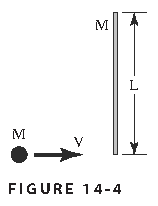
\includegraphics[width=0.86\linewidth,height=0.42\textheight,keepaspectratio]{../assets/pdf-layer-figures/fig-14_4-p189.pdf}

\par{\scriptsize Рисунок 14-4 (исходная стр. 189)}

\end{center}

\begin{center}

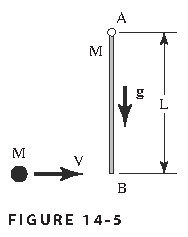
\includegraphics[width=0.86\linewidth,height=0.42\textheight,keepaspectratio]{../assets/pdf-layer-figures/fig-14_5-p189.pdf}

\par{\scriptsize Рисунок 14-5 (исходная стр. 189)}

\end{center}

\begin{center}

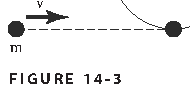
\includegraphics[width=0.86\linewidth,height=0.42\textheight,keepaspectratio]{../assets/pdf-layer-figures/fig-14_3-p189.pdf}

\par{\scriptsize Рисунок 14-3 (исходная стр. 189)}

\end{center}



И З Б Р А Н Н Ы Е  З А Д А Ч И • 1 7 3 \emph{ } * 1 4 - 7 Вертикально стоящему стержню массы M и длины L сообщают в его основании импульс J, направленный под углом вверх к горизонту, отчего стержень взлетает. Какое значение (или значения) должен иметь импульс J, чтобы стержень снова приземлился вертикально (т. е. вертикально на тот же конец, к которому был приложен импульс J)? 45° Р И С У Н О К  1 4 - 6 Р И С У Н О К  1 4 - 7 L J r \emph{ } 1 4 - 6 На покоящемся поворотном диске T2 смонтирован поворотный диск T1, вращающийся с угловой скоростью ω. В некоторый момент времени внутреннее сцепление воздействует на ось T1, чтобы остановить его относительно T2, но T2 может свободно вращаться. Один только T1 имеет массу M1 и момент инерции I1 относительно оси A1, проходящей через его центр перпендикулярно его плоскости; а диск T2 имеет массу M2 и момент инерции I2 относительно аналогично расположенной оси A2; расстояние между A1 и A2 равно r. Найдите угловую скорость для T2 после остановки T1. (ω --- угловая скорость T1.)\par

\begin{center}

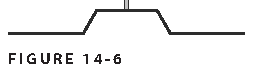
\includegraphics[width=0.86\linewidth,height=0.42\textheight,keepaspectratio]{../assets/pdf-layer-figures/fig-14_6-p190.pdf}

\par{\scriptsize Рисунок 14-6 (исходная стр. 190)}

\end{center}

\begin{center}

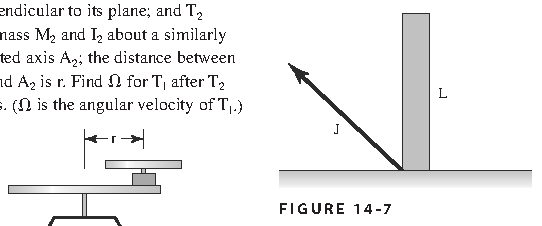
\includegraphics[width=0.86\linewidth,height=0.42\textheight,keepaspectratio]{../assets/pdf-layer-figures/fig-14_7-p190.pdf}

\par{\scriptsize Рисунок 14-7 (исходная стр. 190)}

\end{center}



174 • ГЛАВА 5 \emph{ } * 14-8 Поворотный круг с моментом инерции \(I_0\) свободно вращается вокруг полой вертикальной оси. Тележка массы m движется без трения по прямой радиальной направляющей на поворотном круге. Нитка, прикрепленная к тележке, перекинута через небольшой блок, а затем спускается вниз через полую ось. Вначале вся система вращается с угловой скоростью \(v_0\), а тележка удерживается на фиксированном расстоянии R от оси. Затем тележку подтягивают внутрь, прикладывая к нити дополнительную силу, и в конце концов она останавливается на радиусе r, где её и оставляют. а) Чему равна новая угловая скорость системы? б) Подробно покажите, что разность энергий системы в этих двух состояниях равна работе, совершенной центростремительной силой. в) Если отпустить нить, с какой радиальной скоростью \(dr/dt\) тележка пройдет радиус R?\par



\emph{ } * 14-9 Маховик, имеющий форму однородного тонкого круглого диска массой 10,0 кг и радиусом 1,00 м, установлен на валу, проходящем через его ЦМ, но образующем угол 1°0' с его плоскостью. Если он вращается вокруг этой оси с угловой скоростью 25,0 рад/с, какой вращающий момент должен создаваться подшипниками?\par



РИСУНОК 14-8\par

\begin{center}

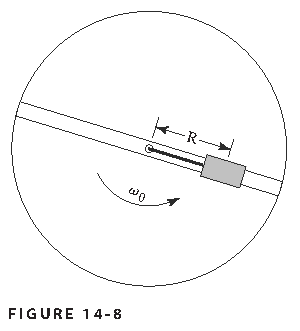
\includegraphics[width=0.86\linewidth,height=0.42\textheight,keepaspectratio]{../assets/pdf-layer-figures/fig-14_8-p191.pdf}

\par{\scriptsize Рисунок 14-8 (исходная стр. 191)}

\end{center}



ИЗБРАННЫЕ УПРАЖНЕНИЯ • 175\par



Ответы к упражнениям Ответы к избранным упражнениям\par



\TipsSubsection{1-1 1-2 1-3 1-4 а) б) в) Нет 1-5 1-6 2 тс 1-7 1-8 1-9 \(v = \sqrt{2gH}\) \(W = 4w\) \(\sin u\) \(u = 30°\) \(u = 30°\) \(t_1 = \sqrt{\frac{2H}{g (a_1 - 1/\sqrt{2})}}\) \(a = 2 \left(1 - \frac{1}{\sqrt{2}}\right) g\) \(F = W \frac{\sqrt{h(2R - h)}}{R - h}\) \(B = \frac{\sqrt{3}}{2}\) кгс \(A = \left(1 - \frac{\sqrt{3}}{2}\right)\) кгс \(F_W = \tan \alpha\) кгс \(F_P = \frac{1}{\cos \alpha}\) кгс}



\TipsSubsection{2-1 1.033 2-2 а) б)}



\TipsSubsection{3-1 а) б) 3-2 3-3 вниз 3-4 3-5 3-6 а) б) 3-7}



\TipsSubsection{4-1 4-2 4-3 \(g = \frac{v^2(2M + m)}{2mh}\) \(F = \frac{M_2 - M_1}{M + M_1 + M_2} g\) \(T = 25\) Н \(a_J = \frac{8}{9} a_R\) 2.75 фут/с² 52.5 миль/ч 14.8 м/с \(e < 0.98\) \(<155\) с \(v < 1385\) фут/с \(t = 1843.8\) с \(r_s = \frac{1}{9} r_{em}\) \$l = 0}



176 • ГЛАВА 5\par



\TipsSubsection{4-4 а) б) 280 фунтов 4-5}



\TipsSubsection{5-1 5-2 а) Да б) На север в) 5-3 5-4 5-5 5-6}



\TipsSubsection{6-1 Способ 2, на 4.0 мин. 6-2 \(t_A / t_L = t_V / t_A\) \(t_A / t_V = V / \sqrt{V^2 - v^2}\) \(F_R \sim 2v^2\) \(F_R = 5.1 \times 10^{-3}\) Н \(\Delta v < v/4\) \(V = x \frac{m + M}{m} \sqrt{\frac{g}{L}}\) \(F = mv_1(v + gt)\)? [или \(F = m(v_1 + gt)\)] \(V = 5 \times 10^{-4}\) м/с \(m_2/m_1 = 3\) \(m_B \approx 5.8\) кг \$a\_\{\(\text{вверх}\)\} = g/3}



\TipsSubsection{6-3 6-4 а) на север б) 0.17 ч}



\TipsSubsection{7-1 7-2 7-3}



\TipsSubsection{8-1 8-2 8-3 51.8 миль/ч 8-4 Ускоряется 8-5 а) б)}



\TipsSubsection{9-1 \(x_0 - x = x_0 - v_0 \sqrt{\frac{m}{k}}\) \(\phi = 60°\) \(\sqrt{3} W \sin \alpha\) \(a = \frac{g}{\sqrt{3}}\) м/с² \(v_0 = 595\) м/с \(a = 2g\) 8 \(M/m_P = 9\) \(\left( \frac{\Delta T}{T} \right)_{\text{лаб}} = \frac{(1 - a^2) m_2}{m_1 + m_2}\) \(u_{\text{max}} = \arcsin(m/M)\) \$T = 2\emph{p} \textbackslash{}sqrt\{\(\frac{H}{g}\)\}}



ИЗБРАННЫЕ УПРАЖНЕНИЯ • 177\par



\TipsSubsection{9-2 В любом месте 9-3 9-4 9-5 9-6 9-7 9-8 9-9 Спутник улетит по параболической орбите.}



10-1 10-2 T не зависит от k. \(E_r = m l^2 \dots\) \(F_r = m l \dots\) \(a_r = l \dots\) \(v_r = l \dots\) \(\approx 330\) Дж \(\approx 570\) Дж \(\approx 625\) Дж 7.2 м/с² \(v = \sqrt{\frac{3gL}{2}}\) \(H = \frac{1}{2} R\) \(v \approx 3.9\) миль/с\par



11-1 а) б) 11-2 11-3 а) б) 11-4\par



\[12-1 12-2 M = 4.0 \text{фунта 12-3 }n = a x = \frac{m_1}{m_1 + m_2} L (\text{от }m_2) h = a \frac{3 - \sqrt{3}}{2} y = \frac{1}{2} x x = 1.7 \text{см 12-4 12-5 }E_g = 4 m_p c^2 (3.8 \text{ГэВ) }\frac{4}{\sqrt{3}} m c/2 p_{\mu} = p_{\nu} = 29.7 \text{МэВ/}c T_{\nu} = 29.7 \text{МэВ }T_{\mu} = 4.1 \text{МэВ }v/c = \sqrt{3}/2 pc = T \left( 1 + \frac{2m_0c^2}{T} \right)^{1/2} 12-6\]



178 • ГЛАВА 5\par



13-1 13-2 13-3 13-4 13-5 13-6 13-7 13-8 а) б)\par



\[14-1 (\text{д) 14-2 а) до б) (где }l — \text{длина нити) }V_{CM} = \frac{v_0}{2}, v = v_0 V_0 = \frac{1}{4} R v_0 V_0 = \frac{2}{5} R v_0 V = \frac{5}{7} V_0 D = \frac{12 V_0^2}{49 g} h = \frac{3d}{2} - 3r a = 2g \sin \theta V_0 = r \sqrt{\frac{2Mgh}{I + Mr^2}} F = \frac{Mg}{4} a = \frac{mg}{m + M/2} I = \frac{mL^2}{12}\]



14-3 14-4 а) б) в) г) 20\% 14-5 14-6 14-7 14-8 а) \(v = v_0 \frac{I_0 + mR^2}{I_0 + mr^2}\) б) (Ответ не приводится.) в) \(v = v_0 \sqrt{\frac{I_0 + mR^2}{I_0 + mr^2} (R^2 - r^2)}\)\par



14-9 \(T \approx 27\) Н\ensuremath{\cdot}м \(J = M \sqrt{\frac{\pi g L}{3 n}}\) (n --- целое число) \(V = \frac{I_2}{I_1 + I_2 + Mr^2} v\) \(V = \frac{\sqrt{8gL}}{6}\) \(v = \frac{5}{6} \frac{v}{L}\)? \(MvL/4\) \(v_2\) Кин. энергия = \(\frac{2}{3} mv^2\) Кин. энергия = \(\frac{1}{2} mv^2\) \(v = v/3R\) \(L = mvR/2\) \(V_{CM} = v/2\)\par



\clearpage

\phantomsection

\section*{Источники иллюстраций}

\addcontentsline{toc}{section}{Источники иллюстраций}

\pdfbookmark[1]{Источники иллюстраций}{tips-sec-14-источники-иллюстраций}

\label{tips-sec-14-источники-иллюстраций}

\markboth{Источники иллюстраций}{Источники иллюстраций}

Источники иллюстраций Стр. xi, Фейнман, около 1962 г. (фотограф неизвестен), любезно предоставлено Ральфом Лейтоном Стр. 70, Библиотека редких книг и рукописей имени Джин Эштон, Библиотека Батлера, шестой этаж, Колумбийский университет, 535 West 114th Street, New York, NY 10027 Стр. 112, Физический факультет Бристольского университета Стр. 124, Калифорнийский технологический институт\par



\clearpage

\phantomsection

\section*{Предметный указатель}

\addcontentsline{toc}{section}{Предметный указатель}

\pdfbookmark[1]{Предметный указатель}{tips-sec-15-предметный-указатель}

\label{tips-sec-15-предметный-указатель}

\markboth{Предметный указатель}{Предметный указатель}

Предметный указатель ускорение, 63, 66 акселерометры, 131 момент количества движения, 89, 142 в астрономии, 145 в квантовой механике, 147 угловая скорость, 142 авиагоризонт, 118 атомное ядро, открытие, 99 вавилонская математика, 69 Ванна, 139 Калтех советы студентам, 36 фейнмановские лекторы, 23 программа обучения физике в бакалавриате, 29 столкновения частиц, 64 дифференцирование, 39 векторов, 49 гирополукомпас, 117 диск, вращающийся, 142 Земля вращение, 139 прецессия, 141 нутация, 145 сплюснутость, 140 электричество, 68 электрон, 147 энергия, 62 сохранение, 62, 63, 84, 85, 93, 112 кинетическая, 63 нейтрино, 112 фотона, 108 потенциальная, 64, 67 полная, 62 скорость освобождения, 84, 93 обратная связь, 127 «Фейнмановские лекции по физике» цель, 7, 13, 29 преподавание, 23 стенограмма, 9, 23 использование, 32 Фейнман, Ричард Ф. интервью, 15 структура лекций, 16 принципы преподавания, 16 стиль преподавания, 7 сила, 61, 67 при малых скоростях, 63 консервативная, 64 трение, 68 гравитация между частицами, 67 на Земле, 67 потенциал, 67, 68 гирокомпас, 120 гироскоп калибровка, 130, 138 демонстрация, 116 усовершенствования, 124 с одной степенью свободы, 125, 129 судовой стабилизатор, 119 инерциальная навигация, 115 интегрирование, 42 криволинейные интегралы, 51 камневые опоры, 126 законы Кеплера, 92 Лейтон, Роберт Б. интервью, 23 физические задачи, 155\par



1 8 2 • ПРЕДМЕТНЫЙ УКАЗАТЕЛЬ Лейтон, Роберт Б. (продолжение) руководитель программы, 30 как преподаватель, 23 логарифм, натуральный, 104 проектирование машин, 73 заучивание (формул), 58, 69 момент инерции, 142 импульс и сила, 61 при малых скоростях, 63 сохранение, 62, 63, 112 нейтрино, 112 фотона, 108 Луна, сплюснутость, 140 туманности, 146 «Наутилус» (подводная лодка), 115, 138 навигационная система, полная, 135 численное интегрирование, 102 орбиты эллиптические, 92 гиперболические, 96 физические законы, 61, 66 нерелятивистское приближение, 63, 66 физика, физическое понимание, 70 пи-мезон, 111 мощность, 79 главные оси, 142 дефлектор протонного пучка, 108 ракеты, 100 химические, 104 основное уравнение, 100 ионные двигатели, 105 фотонные двигатели, 108 динамика вращательного движения, 115 Резерфорд, Эрнест, 99 Сэндс, Мэттью и Фейнман, 8, 13, 24 интервью, 29 воспоминания, 1 движение спутников, 91 датчик сигналов, 125, 127 пружина, идеальная, 68 стабилизированная платформа, 127, 135 тяга, 105 отношение тяги к мощности, 107 момент силы, 89 датчик момента, 127 триангуляция (знаний), 58 векторы, 44 сложение, 44 компоненты, 46, 50, 55 дифференцирование, 49 скалярное произведение, 48 положение, 44 радиус-вектор, 49 вычитание, 44 вектор скорости, 49 Фогт, Рохус Э. интервью, 29 физические задачи, 155 напряжение, 110 ветер, 140 работа, 64 Загружено [stormrg]\par



\clearpage

\phantomsection

\section*{Атлас рисунков}

\addcontentsline{toc}{section}{Атлас рисунков}

\pdfbookmark[1]{Атлас рисунков}{tips-figure-atlas-ru}

\begin{center}

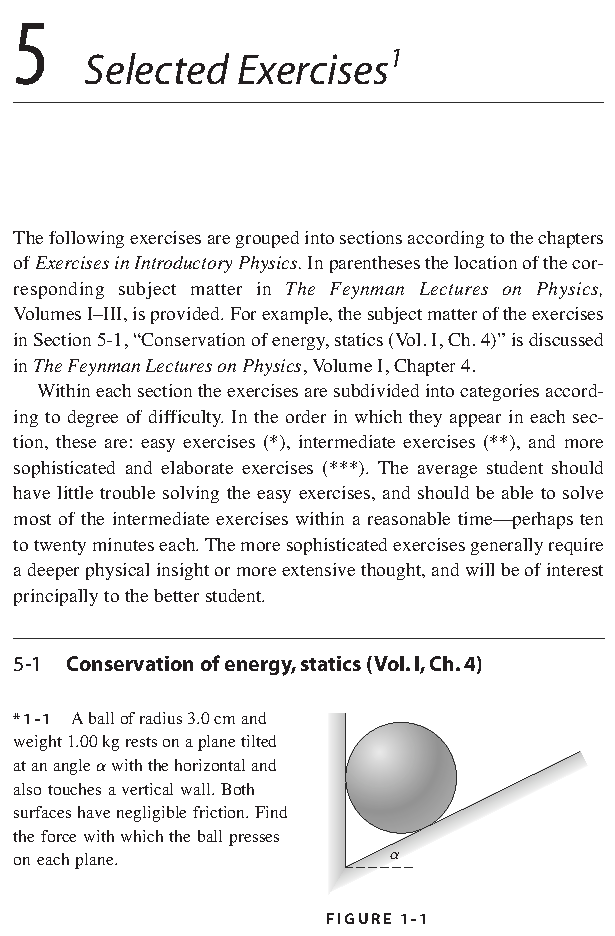
\includegraphics[width=0.92\linewidth,height=0.72\textheight,keepaspectratio]{../assets/pdf-layer-figures/fig-1_1-p172.pdf}

\par{\footnotesize\bfseries Рисунок 1-1 (исходная стр. 172)}

\end{center}

\vspace{4bp}

\begin{center}

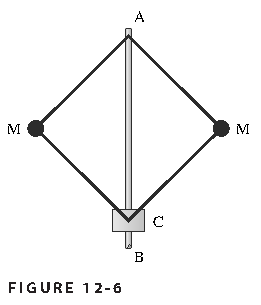
\includegraphics[width=0.92\linewidth,height=0.72\textheight,keepaspectratio]{../assets/pdf-layer-figures/fig-12_6-p186.pdf}

\par{\footnotesize\bfseries Рисунок 12-6 (исходная стр. 186)}

\end{center}

\vspace{4bp}

\end{document}
